% +--------------------------------------------------------------------+
% | Chapter 05 - Characterization of (S,N)-implications 			   |
% +--------------------------------------------------------------------+

\graphicspath{{./_figures/05_snimplications/}}

\section{Introduction}\label{section:introduction}
The family of $(S,N)$-implications where $S$ is a t-conorm and $N$ is a fuzzy negation has attracted the attention and efforts of the fuzzy logic community since the first studies on fuzzy implication functions (see \cite{Dubois1999,Fodor1994,Klir1995,Trillas1985} and references therein). This interest was originated from the fact that $(S,N)$-implications are the straightforward generalization of the classical material implication given by $p\rightarrow q \equiv \neg p \vee q$ to fuzzy logic, where the binary disjunction $\vee$ is modeled by means of a t-conorm $S$ and the classical negation $\neg$ is modeled through a fuzzy negation $N$. This family of fuzzy implication functions was studied at first under very strong assumptions where either $N$ was considered as a strong negation (leading to the so-called $S$-implications) or $S$ was a continuous t-conorm. However, the definition of $(S,N)$-implications without any further assumption is the one usually considered nowadays (see \cite{Baczynski2008,Baczynski2015,Mas2007} and references therein).

The axiomatic characterization of $(S,N)$-implications has been a recurrent line of research for the last decades. A first step was done by Trillas and Valverde in \cite{Trillas1985}, where a characterization of $S$-implications was presented. Subsequently, Baczy\'nski and Jayaram in \cite{Baczynski2007} characterized the family of $(S,N)$-implications when $N$ is a continuous fuzzy negation. Moreover, Massanet and Torrens provided alternative characterizations of $(S,N)$-implications when $N$ is a continuous fuzzy negation based on the law of importation in \cite{Massanet2011B}. However, up to our knowledge no further advances have been achieved in the last decade and the characterization of $(S,N)$-implications when $N$ is a non-continuous negation remains an open problem \cite{Baczynski2008,Baczynski2015}.

This chapter contains new advances on the open problem of the characterization of $(S,N)$-implications when $N$ is a non-continuous negation. The non-continuity of the fuzzy negation means the loss of several properties that are repeatedly used in the characterization when the continuity of $N$ is assumed, and this fact drastically increases the difficulty of the problem in the non-continuous case. Indeed, when $N$ is not continuous: (i) $(S,N)$-implications are not generated from a unique pair $(S,N)$; (ii) the modified pseudo-inverse of $N$ is not defined; (iii) there are values of $S$ which are not used to generate the $(S,N)$-implication. Therefore, these difficulties have to be adequately handled at first in any attempt to achieve a characterization. The complexity resulting from observation (iii) has to be stressed. In other words, the expression of any $(S,N)$-implication does not provide any explicit information about the values of $S$ in a certain subregion of $[0,1]^2$. Therefore, the characterization problem is inevitably associated with the problem of the completion of a binary function defined on $A\subsetneq [0,1]^2$ to a t-conorm defined on the whole unit square. In accordance, the first result of this chapter is the equivalence between these two problems, which results in a first characterization of $(S,N)$-implications when $N$ is a non-continuous negation. However, this characterization relies on the possible completability of a t-conorm only determined in a subregion region of $[0,1]^2$ which depends on the range of $N$. This condition is neither simple or verifiable without further study, so with the aim of providing another characterization of $(S,N)$-implications based on the explicit construction of the t-conorm $S$ we focus on the completion problem.

The dual problem of the completion of a binary function defined on $A\subsetneq [0,1]^2$ to a t-norm is a classical problem in the study of these operators \cite{Kimberling1973}. Typically, the problem is studied for continuous operators and, more specifically, for continuous Archimedean t-norms, since in the latter case the problem is equivalent to the study of the existence and uniqueness of additive generators, up to a multiplicative constant. Thus, in the Archimedean case the problem commonly is reduced to the study of different functional equations. For instance, continuous Archimedean t-norms only known in the diagonal or a vertical/horizontal section are linked to the well-known Schröder and Abel functional equations, respectively \cite{Alsina2006}. However, depending on the region, the result and resolution of the problem can change drastically. Up to now, many regions have been considered for this problem \cite{Alsina2006,Bezivin1993,Darsow1983,Jenei2005,Kimberling1973,Klement1999,Mesiar1999,Mesiarova2017} and in this chapter we provide a survey on the topic. The completion problem is interesting since it highlights important properties of these operators. For instance, this type of results underline parts of the operator which, together with the properties in the definition, uniquely define all the other values. This kind of information helps to achieve a better understanding of the structure of t-norms. Also, it can be of practice in real-life situations when a part of the t-norm is fixed by the restriction of a particular problem \cite{Mesiarova2017}.

In view of the duality between t-norms and t-conorms and our proof of the equivalence between the characterization of $(S,N)$-implications and the completion of t-conorms, in this chapter we have introduced another motivation for the study of the completions of t-norms. Three conclusions can be drawn from the study of the literature: (i) the literature focuses on continuous t-norms and, more specifically, on continuous Archimedean t-norms; (ii) the completion problem is not trivial, and its study is very different depending on the considered region; (iii) the regions of interest for the characterization of $(S,N)$-implications have not been previously studied. Consequently, as a first step we have restricted ourselves to the case when $S$ is a continuous t-conorm and $N$ has one point of discontinuity. These assumptions lead to the study of the completions of continuous t-norms, which can be unknown in eight different types of subregions of $[0,1]^2$ that are determined by the kind of point of discontinuity the fuzzy negation $N$ has.

The problem of determining the completions of continuous t-norms unknown in the eight different regions derived from the characterization of $(S,N)$-implications when $N$ has one point of discontinuity is deeply studied and all the corresponding completions are explicitly constructed. For the resolution of this problem, it has been necessary to make an exhaustive and long study in which different cases depending on the region and the characteristics of the t-norm had to be considered. Moreover, different and specific strategies were necessary for solving the problem in several of these cases. Therefore, independently from the characterization of $(S,N)$-implications, the resolution of this problem includes new results in the study of the structure of continuous t-norms.

Finally, we use the obtained results on the completion of continuous t-norms to provide a second characterization of $(S,N)$-implications where $S$ is the maximum or a continuous Archimedean t-conorm and $N$ has one point of discontinuity, in which the explicit construction of the corresponding t-conorm $S$ is provided.

The structure of the chapter is as follows. In Section \ref{section:objectives&problems} the characterization of $(S,N)$-implications when $N$ is a continuous negation is studied in detail, its several parts are broken into pieces and compared with the case when $N$ is not continuous. In Section \ref{section:characterization1}, a first general characterization of $(S,N)$-implications when $N$ is a non-continuous negation is presented, proving the connection of this problem with the completion problem. In Section \ref{section:completions} we study the completion of binary functions defined on the eight regions of interest to continuous t-norms. In Section \ref{section:characterization2} we use the results of the previous two sections to present another characterization of the $(S,N)$-implications when $S$ is the maximum or a continuous Archimedean t-conorm and $N$ has a unique point of discontinuity. The chapter ends in Section \ref{section:sn:conclusions} with some conclusions and future work.

\section{Discussion and previous considerations}\label{section:objectives&problems}
First of all, we analyze the characterization of $(S,N)$-implications when $N$ is a continuous negation in order to identify which problems arise when facing the non-continuous case. The available characterization provided in \cite{Baczynski2007} (and recalled here in Theorem \ref{th:charac_(S,N)_Ncont}) relies on the continuity of $N$ in two different ways:
\begin{itemize}
	\item The continuity of $N$ ensures that an $(S,N)$-implication is generated by a unique pair (t-conorm $S$, fuzzy negation $N$).
	\item The modified pseudo-inverse of $N$ is a fuzzy negation and it satisfies two useful equalities ((iii) and (iv) in Proposition \ref{prop:properties_modifiedpseudoinverse}). As it can be seen in Theorem \ref{th:charac_(S,N)_Ncont}, this modified pseudo-inverse is used in the construction of $S$ based on the values of $N$ and $I$.
\end{itemize}
In the case when $I$ is an $(S,N)$-implication with a non-continuous negation $N$, we deal with the following problems:
\begin{enumerate}[label=\arabic*.]
	\item The construction of an $(S,N)$-implication $I$ as $S(N(x),y)$ may not be unique. Many t-conorms can generate the same $I$.
	\item Although the modified pseudo-inverse defined as Equation (\ref{eq:modified_pseudoinverse_negation}) is a fuzzy negation even when $N$ is not continuous, it does not satisfy Equalities (\ref{eq:PropositionRN(iii)}) and (\ref{eq:PropositionRN(iv)}) in general.  Therefore, in order to provide a similar characterization in the non-continuous case we need to consider an alternative to the modified pseudo-inverse. Moreover, this alternative must have similar properties to the modified pseudo-inverse in order to be useful in the proof of the characterization.
	\item If $N$ is non-continuous, then there are values of the t-conorm $S$ that are not used in the construction of the corresponding $(S,N)$-implication. Therefore, it may not be always possible to determine $S$ on the whole square $[0,1]^2$ from the values of $I$ and $N$. 
\end{enumerate}

Taking into account the above facts, before providing a characterization of $(S,N)$-implications when $N$ is a non-continuous negation we need to deeply analyze the three arising problems.

\subsection{Non-unicity of the t-conorm $S$}\label{subsection:equivalence-relation}

From the construction of $(S,N)$-implications (see Definition \ref{def:(S,N)}) it is straightforward to see that when $N$ is a non-continuous negation then an $(S,N)$-implication need not to be given by a unique $S$. Let us illustrate this fact by providing an example.

\begin{example}\label{Ex:NoUnicityS}
	Let us consider the following non-continuous fuzzy negation
	$$N(x) = \left\{\begin{array}{ll}
		1-x & \text{ if } x \in [0,0.25]\cup[0.75,1], \\
		0.25 & \text{ if } x \in (0.25,0.75). 
	\end{array}
	\right. 
	$$
	For any t-conorm $S$, the corresponding $(S,N)$-implication is
	$$
	S(N(x),y)
	=
	\left\{\begin{array}{ll}
		S(1-x,y) & \text{ if } x \in [0,0.25]\cup[0.75,1] \text{ and } y \in [0,1], \\
		S(0.25,y) & \text{ if } x \in (0.25,0.75) \text{ and } y \in [0,1]. 
	\end{array}
	\right.
	$$
	We point out that the only values of $S$ that are used in the expression above are $(x,y) \in ([0,0.25]\times [0,1]) \cup ([0.75,1] \times [0,1])$. Therefore, using any t-conorm with the same values in this region results in the same $(S,N)$-implication. For instance, if we consider the following continuous t-conorms
	$$S_1(x,y)=\max\{x,y\}, \quad (x,y)\in[0,1]^2,$$
	$$S_2(x,y)= \left\{\begin{array}{ll}
		1.5x+1.5y-2xy-0.375 & \text{ if } (x,y) \in (0.25,0.75)^2, \\
		\max\{x,y\} & \text{otherwise}, 
	\end{array}
	\right.
	$$
	we obtain the same $(S,N)$-implication:
	\begin{equation}\label{eq:example1}
		I_{S_1,N}(x,y)=I_{S_2,N}(x,y)= \left\{\begin{array}{ll}
			\max\{1-x,y\} & \text{ if } x \in [0,0.25] \cup [0.75,1] \text{ and } y \in [0,1], \\
			\max\{0.25,y\} &  \text{ if } x \in (0.25,0.75) \text{ and } y \in [0,1].
		\end{array}
		\right.
	\end{equation}
	Indeed, Figure \ref{fig:1} emphasizes that $S_1$ and $S_2$ are different in $(0.25,0.75)^2$ and yet generate the same $(S,N)$-implication.
	\begin{figure}[H]
		\centering
		\begin{subfigure}{.25\textwidth}
			\centering
			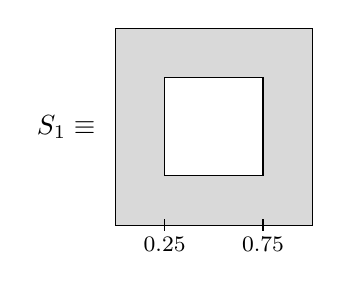
\begin{tikzpicture}[xscale=2.5, yscale=2.5]
				\node at (-0.25,0.5) {$S_1 \equiv$};
				\draw[fill=gray!30] (0,0) rectangle (1,1);
				\draw[fill=white!30] (0.25,0.25) rectangle (0.75,0.75);
				\node at (0.5,0.5) {\SM};
				\node at (0.15,0.85) {\SM};
				\draw (0.25,-0.03)--(0.25,0.03);
				\node at (0.25,-0.1) {\footnotesize 0.25};
				\draw (0.75,-0.03)--(0.75,0.03);
				\node at (0.75,-0.1) {\footnotesize 0.75};
			\end{tikzpicture}
		\end{subfigure}%
		\hspace{1cm}
		\begin{subfigure}{.25\textwidth}
			\centering
			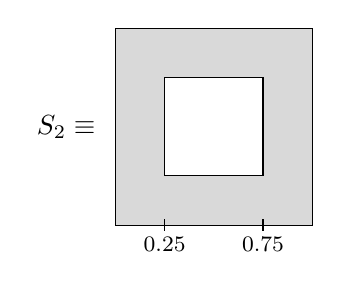
\begin{tikzpicture}[xscale=2.5, yscale=2.5]
				\node at (-0.25,0.5) {$S_2 \equiv$};
				\draw[fill=gray!30] (0,0) rectangle (1,1);
				\draw[fill=white!30] (0.25,0.25) rectangle (0.75,0.75);
				\node at (0.5,0.5) {\SP};
				\node at (0.15,0.85) {\SM};
				\draw (0.25,-0.03)--(0.25,0.03);
				\node at (0.25,-0.1) {\footnotesize 0.25};
				\draw (0.75,-0.03)--(0.75,0.03);
				\node at (0.75,-0.1) {\footnotesize 0.75};
			\end{tikzpicture}
		\end{subfigure}%
		\caption[Schema of the structure of two t-conorms that generate the same $(S,N)$-implication.]{Schema of the structure of two t-conorms that generate the same fuzzy implication function in Equation (\ref{eq:example1}), where the values that are used for that construction are shaded in gray.}\label{fig:1}
	\end{figure}
\end{example}

The non-unicity shown in the previous example is formalized in the following proposition.
\begin{proposition}\label{prop:non-unicity}
	Let $N_1$ and $N_2$ be two fuzzy negations and $S_1$ and $S_2$ be two t-conorms. Then, the following statements are equivalent:
	\begin{enumerate}[label=(\roman*)]
		\item $I_{S_1,N_1}(x,y)=I_{S_2,N_2}(x,y)$ for all $x,y \in [0,1]$.
		\item $N_1(x)=N_2(x)=N(x)$ for all $x \in [0,1]$ and $S_1(x,y)=S_2(x,y)$ for all $(x,y) \in (\Ran N \times [0,1]) \cup (([0,1] \setminus \Ran N) \times \Ran N)$.
	\end{enumerate}
\end{proposition}
\begin{proof}
	Let us assume that $I_{S_1,N_1}(x,y)=I_{S_2,N_2}(x,y)$ for all $x,y \in [0,1]$. Then, for all $x\in[0,1]$ $$N_1(x)=S_1(N_1(x),0)=I_{S_1,N_1}(x,0)=I_{S_2,N_2}(x,0)=S_2(N_2(x),0)=N_2(x).$$	
	In this case, we define $N(x)=N_1(x)=N_2(x)$ for all $x \in [0,1]$. Now, consider an arbitrary but fixed $x \in \Ran N$. Then, there exists an $x' \in [0,1]$ such that $N(x')=x$ and for all $y \in [0,1]$ we get
	$$S_1(x,y)=S_1(N(x'),y)=I_{S_1,N}(x',y)=I_{S_2,N}(x',y)=S_2(N(x'),y)=S_2(x,y).$$
	On the other hand, if $x \in [0,1] \setminus \Ran N$ and $ y \in \Ran N$ there exists a $y' \in [0,1]$ such that $N(y')=y$ and we have
	\begin{eqnarray*}
	S_1(x,y) &=&S_1(y,x)=S_1(N(y'),x)=I_{S_1,N}(y',x)\\
	&=&I_{S_2,N}(y',x)=S_2(N(y'),x)=S_2(y,x)=S_2(x,y).
	\end{eqnarray*}
	For the reverse implication, for all $x,y \in [0,1]$ we have
	$$I_{S_1,N_1}(x,y)=S_1(N_1(x),y)=S_2(N_2(x),y)=I_{S_2,N_2}(x,y).$$
\end{proof}
Notice that if two $(S,N)$-implications are equal, they are necessarily generated by the same fuzzy negation $N$ but their corresponding t-conorms only need to be equal in the region $(\Ran N \times [0,1]) \cup (([0,1] \setminus \Ran N) \times \Ran N)$. Due to this fact, we define the following binary relation on the set of all t-conorms.
\begin{definition} Let $N$ be a fuzzy negation and $S_1$, $S_2$ two t-conorms. Then we define the relation $\equiv_N$ as	
	$$S_1 \equiv_N S_2 \Leftrightarrow I_{S_1,N}(x,y)=I_{S_2,N}(x,y), \quad \text{for all } x,y \in [0,1].$$
	In this case we say that $S_1$ is \emph{$N$-equivalent} to $S_2$. If $S$ is a t-conorm, we define
	$$[S]_N = \{S^* \text{ is a t-conorm } \mid S^* \equiv_N S\}.$$
\end{definition}
It is straightforward to prove that the relation $\equiv_N$ is an equivalence relation and, if $N$ is a continuous negation then two t-conorms are related if and only if they are equal.

\begin{lemma}
Let $N$ be a fuzzy negation and $S_1$, $S_2$ two t-conorms. Then,
	\begin{enumerate}[label=(\roman*)]
		\item $\equiv_N$ is an equivalence relation.
		\item If $N$ is continuous, then $S_1 \equiv_N S_2 \Leftrightarrow S_1(x,y)=S_2(x,y),$ for all $x,y \in [0,1]$.
	\end{enumerate}
\end{lemma}
\begin{proof}
	\begin{enumerate}[label=(\roman*)]
		\item Straightforward since the relation is defined by means of an equality.
		\item If $N$ is continuous, then $\Ran N = [0,1]$ and the result follows by Proposition \ref{prop:non-unicity}.
	\end{enumerate}
\end{proof}

According to this notation, in order to give a detailed description of a certain $(S,N)$-implication $I$ we need to determine the negation $N$ and all the t-conorms that generate $I$, i.e., all the t-conorms in the equivalence class $[S]_N$. For the particular case of continuous t-conorms we provide the definition of the equivalence classes restricted to the set of all continuous t-conorms.

\begin{definition} Let $N$ be a fuzzy negation and $S$ a continuous t-conorm. We define
	$$[S]_N^C = \{S^* \text{ is a continuous t-conorm} \mid S^* \equiv_N S \}.$$
\end{definition}


\subsection{Definition of \RN for a non-continuous negation $N$}\label{subsection:RN}

In the characterization of $(S,N)$-implications based on a continuous negation $N$, one of the key points is that the function $\mathfrak{R}_N$ satisfies the properties from Proposition \ref{prop:properties_modifiedpseudoinverse}. Thanks to these good properties, and especially thanks to Equations (\ref{eq:PropositionRN(iii)}) and (\ref{eq:PropositionRN(iv)}), the authors in \cite{Baczynski2007} were able to reconstruct the t-conorm $S$ of the $(S,N)$-implication $I$ from the values of $I$ and $N$. However, when $N$ is a non-continuous negation, Equations (\ref{eq:PropositionRN(iii)}) and (\ref{eq:PropositionRN(iv)}) do not generally hold. As an alternative to the pseudo-inverse, we consider the concept of quasi-inverse of a decreasing function.

\begin{definition}[\bf \cite{Klement1999}]\label{def:quasi-inverse} Let $f:[0,1] \to [0,1]$ be a decreasing function. Each function $f^{*}:[0,1]\to[0,1]$ satisfying
	\begin{enumerate}[label=(\roman*)]
		\item $f \circ f^*|_{\Ran f} = \text{id}|_{\Ran f}$,
		\item $f^{\wedge} \leq f^* \leq f^{\vee}$,
	\end{enumerate}
	is called a \emph{quasi-inverse} of $f$, where  $f^{\wedge}:[0,1] \to [0,1]$ and  $f^{\vee}:[0,1]\to[0,1]$ are defined as 
	$$f^{\wedge}(y)=\sup \{x \in [0,1] \mid f(x)>y\}, \quad f^{\vee}(y)=\inf \{x \in [0,1] \mid f(x)<y\}.$$
\end{definition}

The functions $f^{\wedge}$ (or pseudo-inverse) and $f^{\vee}$ are not quasi-inverses in general (see \cite{Klement1999}). In contrast with the concept of pseudo-inverse, an arbitrary decreasing function $f:[0,1] \to [0,1]$ may have a whole family of quasi-inverses. However, $f$ has at least one quasi-inverse defined in the following proposition.

\begin{proposition}[\bf \cite{Klement1999}]\label{prop:quasi-inverse}
	Let $f:[0,1]\to[0,1]$ be a decreasing function. Then the function $f^{*} = (f^{\wedge}+f^{\vee})/2$ is a quasi-inverse of $f$.
\end{proposition}

\begin{example}\label{Ex:Quasi-inverse}
	Let us consider the following decreasing function
	$$f(x) = \left\{\begin{array}{ll}
		1-x & \text{ if } x \in [0,0.25], \\
		0.25 & \text{ if } x \in (0.25,0.5), \\
		0.5(1-x) & \text{ if } x \in [0.5,1]. 
	\end{array}
	\right. 
	$$
	Then, we have
	$$f^{\wedge}(x) = \left\{\begin{array}{ll}
		1-2x & \text{ if } x \in [0,0.25), \\
		0.25 & \text{ if } x \in [0.25,0.75), \\
		1-x & \text{ if } x \in [0.75,1], 
	\end{array}
	\right. \quad
	f^{\vee}(x) = \left\{\begin{array}{ll}
		1-2x & \text{ if } x \in [0,0.25], \\
		0.25 & \text{ if } x \in (0.25,0.75), \\
		1-x & \text{ if } x \in [0.75,1]. 
	\end{array}
	\right. 
	$$
	Therefore, any function $f^*:[0,1] \to [0,1]$ with $f^*(x)=f^{\wedge}(x)=f^{\vee}(x)$ for all $x \in [0,0.25) \cup (0.25,1]$ and $f^*(0.25) \in (0.25,0.5]$ is a quasi-inverse of $f$. On the other hand, notice that $f \circ f^{\wedge}(0.25)=f(0.25)=0.75 \not = 0.25$. Therefore, in contrast with the quasi-inverses, the pseudo-inverse does not fulfill that $f \circ f^{\wedge}|_{\Ran f} = \text{id}|_{\Ran f}$. See Figure \ref{figure:quasi-inverse} for a graphical representation.
\end{example}

\begin{figure}[H]
	\centering	
	\tikzset{every picture/.style={line width=0.75pt}} %set default line width to 0.75pt        	
	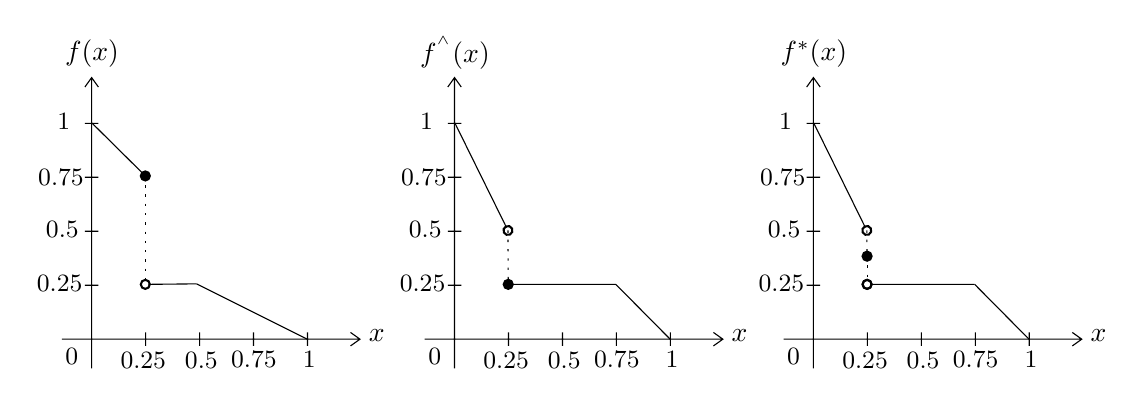
\begin{tikzpicture}[x=0.75pt,y=0.75pt,yscale=-1,xscale=1,scale=0.65]
		%uncomment if require: \path (0,298); %set diagram left start at 0, and has height of 298
		
		%Shape: Axis 2D [id:dp7843255870418544] 
		\draw  (18.61,241.01) -- (239.61,241.01)(40.71,47.1) -- (40.71,262.56) (232.61,236.01) -- (239.61,241.01) -- (232.61,246.01) (35.71,54.1) -- (40.71,47.1) -- (45.71,54.1) (80.71,236.01) -- (80.71,246.01)(120.71,236.01) -- (120.71,246.01)(160.71,236.01) -- (160.71,246.01)(200.71,236.01) -- (200.71,246.01)(35.71,201.01) -- (45.71,201.01)(35.71,161.01) -- (45.71,161.01)(35.71,121.01) -- (45.71,121.01)(35.71,81.01) -- (45.71,81.01) ;
		\draw   ;
		%Straight Lines [id:da531301433026877] 
		\draw    (41,80.85) -- (80.5,120) ;
		\draw [shift={(80.5,120)}, rotate = 44.75] [color={rgb, 255:red, 0; green, 0; blue, 0 }  ][fill={rgb, 255:red, 0; green, 0; blue, 0 }  ][line width=0.75]      (0, 0) circle [x radius= 3.35, y radius= 3.35]   ;
		%Straight Lines [id:da8429477917991068] 
		\draw    (82.85,200.36) -- (118.5,200) ;
		\draw [shift={(80.5,200.38)}, rotate = 359.42] [color={rgb, 255:red, 0; green, 0; blue, 0 }  ][line width=0.75]      (0, 0) circle [x radius= 3.35, y radius= 3.35]   ;
		%Straight Lines [id:da1352257120128888] 
		\draw    (118.5,200) -- (200.5,241) ;
		%Straight Lines [id:da6300820503824969] 
		\draw  [dash pattern={on 0.84pt off 2.51pt}]  (80.5,120) -- (80.5,200.38) ;
		%Shape: Axis 2D [id:dp3200975442932772] 
		\draw  (287.61,241.01) -- (508.61,241.01)(309.71,47.1) -- (309.71,262.56) (501.61,236.01) -- (508.61,241.01) -- (501.61,246.01) (304.71,54.1) -- (309.71,47.1) -- (314.71,54.1) (349.71,236.01) -- (349.71,246.01)(389.71,236.01) -- (389.71,246.01)(429.71,236.01) -- (429.71,246.01)(469.71,236.01) -- (469.71,246.01)(304.71,201.01) -- (314.71,201.01)(304.71,161.01) -- (314.71,161.01)(304.71,121.01) -- (314.71,121.01)(304.71,81.01) -- (314.71,81.01) ;
		\draw   ;
		%Straight Lines [id:da9599616553106449] 
		\draw    (310,80.85) -- (348.25,158.32) ;
		\draw [shift={(349.29,160.43)}, rotate = 63.73] [color={rgb, 255:red, 0; green, 0; blue, 0 }  ][line width=0.75]      (0, 0) circle [x radius= 3.35, y radius= 3.35]   ;
		%Straight Lines [id:da49281738423622] 
		\draw    (349.5,200.38) -- (429.29,200.43) ;
		\draw [shift={(349.5,200.38)}, rotate = 0.03] [color={rgb, 255:red, 0; green, 0; blue, 0 }  ][fill={rgb, 255:red, 0; green, 0; blue, 0 }  ][line width=0.75]      (0, 0) circle [x radius= 3.35, y radius= 3.35]   ;
		%Straight Lines [id:da8562555689616071] 
		\draw    (429.29,200.43) -- (469.5,241) ;
		%Straight Lines [id:da8630706639536878] 
		\draw  [dash pattern={on 0.84pt off 2.51pt}]  (349.29,160.43) -- (349.5,200.38) ;
		%Shape: Axis 2D [id:dp562235776420597] 
		\draw  (553.61,241.01) -- (774.61,241.01)(575.71,47.1) -- (575.71,262.56) (767.61,236.01) -- (774.61,241.01) -- (767.61,246.01) (570.71,54.1) -- (575.71,47.1) -- (580.71,54.1) (615.71,236.01) -- (615.71,246.01)(655.71,236.01) -- (655.71,246.01)(695.71,236.01) -- (695.71,246.01)(735.71,236.01) -- (735.71,246.01)(570.71,201.01) -- (580.71,201.01)(570.71,161.01) -- (580.71,161.01)(570.71,121.01) -- (580.71,121.01)(570.71,81.01) -- (580.71,81.01) ;
		\draw   ;
		%Straight Lines [id:da6439063510838396] 
		\draw    (576,80.85) -- (614.25,158.32) ;
		\draw [shift={(615.29,160.43)}, rotate = 63.73] [color={rgb, 255:red, 0; green, 0; blue, 0 }  ][line width=0.75]      (0, 0) circle [x radius= 3.35, y radius= 3.35]   ;
		%Straight Lines [id:da9312393392247227] 
		\draw    (617.85,200.38) -- (695.29,200.43) ;
		\draw [shift={(615.5,200.38)}, rotate = 0.03] [color={rgb, 255:red, 0; green, 0; blue, 0 }  ][line width=0.75]      (0, 0) circle [x radius= 3.35, y radius= 3.35]   ;
		%Straight Lines [id:da7437300630109214] 
		\draw    (695.29,200.43) -- (735.5,241) ;
		%Straight Lines [id:da5257257030270486] 
		\draw  [dash pattern={on 0.84pt off 2.51pt}]  (615.5,179.5) -- (615.5,198.03) ;
		\draw [shift={(615.5,200.38)}, rotate = 90] [color={rgb, 255:red, 0; green, 0; blue, 0 }  ][line width=0.75]      (0, 0) circle [x radius= 3.35, y radius= 3.35]   ;
		\draw [shift={(615.5,179.5)}, rotate = 90] [color={rgb, 255:red, 0; green, 0; blue, 0 }  ][fill={rgb, 255:red, 0; green, 0; blue, 0 }  ][line width=0.75]      (0, 0) circle [x radius= 3.35, y radius= 3.35]   ;
		%Straight Lines [id:da2525284850658729] 
		\draw    (691,143.29) ;
		%Straight Lines [id:da573874632291911] 
		\draw  [dash pattern={on 0.84pt off 2.51pt}]  (615.29,160.43) -- (615.5,179.5) ;
		
		% Text Node
		\draw (26,253.85) node  [font=\small]  {$0$};
		% Text Node
		\draw (19,159.85) node  [font=\small]  {$0.5$};
		% Text Node
		\draw (18,120.85) node  [font=\small]  {$0.75$};
		% Text Node
		\draw (20,79.85) node  [font=\small]  {$1$};
		% Text Node
		\draw (79,256.85) node  [font=\small]  {$0.25$};
		% Text Node
		\draw (122,256.85) node  [font=\small]  {$0.5$};
		% Text Node
		\draw (161,255.85) node  [font=\small]  {$0.75$};
		% Text Node
		\draw (202,255.85) node  [font=\small]  {$1$};
		% Text Node
		\draw (41,29.18) node    {$f( x)$};
		% Text Node
		\draw (252,238.18) node    {$x$};
		% Text Node
		\draw (17,199.38) node  [font=\small]  {$0.25$};
		% Text Node
		\draw (295,253.85) node  [font=\small]  {$0$};
		% Text Node
		\draw (288,159.85) node  [font=\small]  {$0.5$};
		% Text Node
		\draw (287,120.85) node  [font=\small]  {$0.75$};
		% Text Node
		\draw (289,79.85) node  [font=\small]  {$1$};
		% Text Node
		\draw (348,256.85) node  [font=\small]  {$0.25$};
		% Text Node
		\draw (391,256.85) node  [font=\small]  {$0.5$};
		% Text Node
		\draw (430,255.85) node  [font=\small]  {$0.75$};
		% Text Node
		\draw (471,255.85) node  [font=\small]  {$1$};
		% Text Node
		\draw (310,29.18) node    {$f^{^{\land }}( x)$};
		% Text Node
		\draw (521,238.18) node    {$x$};
		% Text Node
		\draw (286,199.38) node  [font=\small]  {$0.25$};
		% Text Node
		\draw (561,253.85) node  [font=\small]  {$0$};
		% Text Node
		\draw (554,159.85) node  [font=\small]  {$0.5$};
		% Text Node
		\draw (553,120.85) node  [font=\small]  {$0.75$};
		% Text Node
		\draw (555,79.85) node  [font=\small]  {$1$};
		% Text Node
		\draw (614,256.85) node  [font=\small]  {$0.25$};
		% Text Node
		\draw (657,256.85) node  [font=\small]  {$0.5$};
		% Text Node
		\draw (696,255.85) node  [font=\small]  {$0.75$};
		% Text Node
		\draw (737,255.85) node  [font=\small]  {$1$};
		% Text Node
		\draw (576,29.18) node    {$f^{\ast }( x)$};
		% Text Node
		\draw (787,238.18) node    {$x$};
		% Text Node
		\draw (552,199.38) node  [font=\small]  {$0.25$};	
	\end{tikzpicture}
	\caption[Graphical example of the pseudo-inverse and a quasi-inverse of a decreasing function.]{Plot of the function $f$ in Example \ref{Ex:NoUnicityS}, its pseudo-inverse $f^{\wedge}$ and a quasi-inverse $f^{*}$.}
	\label{figure:quasi-inverse}
\end{figure}

If we consider the quasi-inverse from Proposition \ref{prop:quasi-inverse} of an arbitrary fuzzy negation $N$ then (i)-Definition \ref{def:quasi-inverse} is an alternative to Equation (\ref{eq:PropositionRN(iii)}). With respect to Equation (\ref{eq:PropositionRN(iv)}) we can prove only that if an $x \in [0,1]$ does not satisfy Equation (\ref{eq:PropositionRN(iv)}), then we are able to find another point $x^*$ with $N(x)=N(x^*)$ which fulfills Equation (\ref{eq:PropositionRN(iv)}). We will see in Section \ref{section:characterization1} that this fact is sufficient for the characterization of $(S,N)$-implications when $N$ is a non-continuous negation.

\begin{proposition}\label{prop:second-equality}
	Let $f:[0,1] \to [0,1]$ be a decreasing function and $x \in [0,1]$ and $f^{*}$ a quasi-inverse of $f$. If $f^{*} \circ f(x) \not = x$, then there exists an $x^* \in \Ran f^*$ such that $f(x)=f(x^*)$ and $f^* \circ f(x^*)=x^*$.
\end{proposition}
\begin{proof}
	If $f^* \circ f(x) \not = x$, we consider $x^*=f^* \circ f(x) \in \Ran f^*$. Since for a quasi-inverse there is $f \circ f^*|_{\Ran f} = \text{id}|_{\Ran f}$, we have
	$$f(x)=f \circ f^* \circ f(x) = f(f^* \circ f(x))=f(x^*),$$
	and then
	$$f^* \circ f(x^*)=f^* \circ f(x)= x^*.$$
\end{proof}

Notice that a quasi-inverse of a fuzzy negation may not fulfill the boundary conditions and consequently it is not a fuzzy negation, in general. Therefore we introduce the following definition.
\begin{definition} Let $N$ be a fuzzy negation, we define the function $\RN:[0,1] \to [0,1]$ as
	$$
	\RN(x)
	= 
	\left\{ \begin{array}{ll}
		1 &   \text{if }   x=0, \\
		N^*(x) & \text{if } x \in (0,1), \\
		0 & \text{if } x=1,
	\end{array} \right.
	$$
	where $N^*$ is the quasi-inverse of $N$ defined in Proposition \ref{prop:quasi-inverse}.
\end{definition}
From the properties of a quasi-inverse and Proposition \ref{prop:second-equality} we deduce that the function $\RN$ is a fuzzy negation and that it satisfies two useful properties.
\begin{corollary}\label{cor:Nquasiinverseproperties}
	Let $N$ be a fuzzy negation. The following statements hold:
	\begin{enumerate}[label=(\roman*)]
		\item $\RN$ is a fuzzy negation.
		\item $N \circ \RN|_{\Ran N} = \text{id}|_{\Ran N}$.
		\item If $\RN \circ N(x) \not = x$, then there exists an $x^* \in \Ran \RN $ such that $N(x)=N(x^*)$ and $\RN \circ N (x^*)=x^*$.
	\end{enumerate}	
\end{corollary}
\begin{proof} Let $N$ be a fuzzy negation.
	\begin{enumerate}[label=(\roman*)]
		\item Since $N$ is decreasing then $N^*$ is also decreasing (see \cite{Klement1999}). On the other hand, by definition we have $\RN(1)=0$ and $\RN(0)=1$.
		\item If $x=0$ then $N \circ \RN(0)=N(1)=0$ and if $x=1$ then $N \circ \RN(1)=N(0)=1$. Otherwise, the equality follows from (i)-Definition \ref{def:quasi-inverse}.
		\item If $x=0$ then $\RN \circ N(0)=\RN(1)=0$ and if $x=1$ then $\RN \circ N(1)=\RN(0)=1$. Otherwise, the result follows from Proposition \ref{prop:second-equality} and the fact that $0,1 \in \Ran \RN$.
	\end{enumerate}
\end{proof}

\subsection{Towards the construction of a representative}\label{subsection:representative}

In this section we construct a function on $(\Ran N \times [0,1]) \cup (([0,1] \setminus \Ran N) \times \Ran N)$ based on the values of a binary function $I$ and a fuzzy negation $N$, which behaves as a t-conorm if $I$ is an $(S,N)$-implication. As we prove in Section \ref{section:characterization1}, this function plays the role of the t-conorm of the $(S,N)$-implication, however, if $N$ is a non-continuous negation it is defined only on a subregion of $[0,1]^2$.

\begin{definition}\label{def:SIN}
Let $I:[0,1]^2 \to [0,1]$ be a binary function and $N$ a fuzzy negation. Let us define a function $S_{I,N}:A \to [0,1]$ where $A= (\Ran N \times [0,1]) \cup (([0,1] \setminus \Ran N) \times \Ran N)$ as follows
	\begin{equation}\label{eq:SIN}
		\SIN(x,y)
		=
		\left\{ \begin{array}{ll}
			I(\RN(x),y) &   \text{if }   x \in \Ran N \text{ and } y \in [0,1], \\
			I(\RN(y),x) & \text{if } x \in [0,1] \setminus \Ran N \text{ and } y \in \Ran N.
		\end{array} \right.
	\end{equation}
\end{definition}

The following proposition identifies which properties of the binary function $I$ ensure that $S_{I,N}$ has the properties of a t-conorm in the region where it is defined.

\begin{proposition}\label{prop:SIN} Let $I:[0,1]^2 \to [0,1]$ be a binary function and $N$ a fuzzy negation such that $I(\RN(x),y)=I(\RN(y),x)$ for all $x,y \in \Ran N$. Consider $S_{I,N}:A \to [0,1]$ where $A= (\Ran N \times [0,1]) \cup (([0,1] \setminus \Ran N) \times \Ran N)$  as introduced in Definition \ref{def:SIN}. Then, the following statements hold:
	\begin{enumerate}[label=(\roman*)]
		\item $\SIN(x,y)=\SIN(y,x)$ for all $(x,y) \in A$.
		\item If $I$ fulfills \Ione and \Itwo, then \SIN is increasing in each variable.
		\item If $I$ fulfills \NP then $\SIN(x,0)=x$ for all $x \in [0,1]$.
		\item If $I$ satisfies \EP,
		\begin{equation}\tag{\bf R1}\label{eq:R1}
			I(\RN(I(\RN(x),y)),z)=I(\RN(I(\RN(x),z)),y), 
		\end{equation}
		for all $x,y,z \in [0,1]$ such that $x,I(\RN(x),y), I(\RN(x),z) \in \Ran N$ and
		\begin{equation}\tag{\bf R2}\label{eq:R2}
			I(\RN(x),I(\RN(y),z))=I(\RN(I(\RN(x),y)),z), 
		\end{equation}
		for all $x,y,z \in [0,1]$ such that $x, y, I(\RN(x),y) \in \Ran N$,
		then $\SIN(x, \SIN (y,z))=\SIN (\SIN(x,y),z)$ for all $(y,z), (x,\SIN(y,z)), (x,y), (\SIN(x,y),z) \in A$.
	\end{enumerate}
	
\end{proposition}
\begin{proof}\hspace{0.5cm}
	\begin{enumerate}[label=(\roman*)]
		\item Let $(x,y) \in A$. Since $I$ satisfies $I(\RN(x),y)=I(\RN(y),x)$ for all $x,y \in \Ran N$ we have
		\begin{eqnarray*}
			\SIN(x,y)
			&=&
			\left\{ \begin{array}{ll}
				I(\RN(x),y) &   \text{if }   x \in \Ran N \text{ and } y \in [0,1] \setminus \Ran N, \\
				I(\RN(x),y) & \text{if } x,y \in \Ran N, \\
				I(\RN(y),x) & \text{if } x \in [0,1] \setminus \Ran N \text{ and } y \in \Ran N,
			\end{array} \right. \\
			&=&
			\left\{ \begin{array}{ll}
				I(\RN(x),y) &   \text{if }   x \in \Ran N \text{ and } y \in [0,1] \setminus \Ran N, \\
				I(\RN(y),x) & \text{if } x,y \in \Ran N, \\
				I(\RN(y),x) & \text{if } x \in [0,1] \setminus \Ran N \text{ and } y \in \Ran N,
			\end{array} \right. \\
			& = &\SIN(y,x).
		\end{eqnarray*}
		\item Taking into account Point (i) we only need to prove that \SIN is increasing with respect to the second variable, i.e., that $\SIN(x,\cdot)$ is increasing for all $x \in [0,1]$. Let $(x,y_1)$, $(x,y_2) \in A$ with $y_1 < y_2$. We distinguish between two cases depending on the value of $x$:
		\begin{itemize}
			\item If $x \in \Ran N$, since $I$ is increasing with respect to the second variable we have
			$$\SIN(x,y_1) = I(\RN(x),y_1) \leq I(\RN(x),y_2)=\SIN(x,y_2).$$
			\item Let $x \in [0,1] \setminus \Ran N$, then $y_1, y_2 \in \Ran N$  and since $\RN$ is decreasing and $I$ is decreasing with respect to the first variable we have
			$$\SIN(x,y_1) = I(\RN(y_1),x) \leq I(\RN(y_2),x) = \SIN(x,y_2).$$
		\end{itemize}
		\item Let $x \in [0,1]$ then since $I(\RN(y),z)=I(\RN(z),y)$ for all $z,y \in \Ran N$ and $0 \in \Ran N$, we have
		\begin{eqnarray*}
		\SIN(x,0)
		&=&
		\left\{ \begin{array}{ll}
			I(\RN(x),0) &   \text{if }   x \in \Ran N, \\
			I(\RN(0),x) & \text{if } x \in [0,1] \setminus \Ran N,
		\end{array} \right. \\
		&=&
		\left\{ \begin{array}{ll}
		N \circ \RN(x) &   \text{if }   x \in \Ran N, \\
		I(1,x) & \text{if } x \in [0,1] \setminus \Ran N,
	\end{array} \right.
		=x.
		\end{eqnarray*}
		\item Let $x,y,z \in [0,1]$ be such that $(y,z), (x, \SIN(y,z)), (x,y), (\SIN(x,y),z) \in A$. In order to prove that \SIN is associative in the region where it is defined,  we need to distinguish between four cases:
		\begin{itemize}
			\item If $x,y \in \Ran N$  we have two possible cases: 
			\begin{itemize}
				\item If $I(\RN(x),y) \in \Ran N$ then by \Rtwo
				\begin{eqnarray*}
				\SIN(\SIN(x,y),z) &=& I(\RN(I(\RN(x),y)),z)\\
				& = & I(\RN(x),I(\RN(y),z)) =\SIN(x,\SIN(y,z)).
				\end{eqnarray*}
				\item If $I(\RN(x),y) \in [0,1] \setminus \Ran N$ and $z \in \Ran N$, then by \EP and the fact that $I(\RN(y),z) = I(\RN(z),y)$ we have
				\begin{eqnarray*}
					\SIN(\SIN(x,y),z) &=& I(\RN(z),I(\RN(x),y)) = I(\RN(x),I(\RN(z),y)) \\
					&=& I(\RN(x),I(\RN(y),z)) = \SIN (x,\SIN(y,z)).
				\end{eqnarray*}
			\end{itemize}
			\item If $x \in [0,1] \setminus \Ran N$ and $y \in \Ran N$ then $I(\RN(y),z) \in \Ran N$ since otherwise $\SIN(x,\SIN(y,z))$ is not defined. Now we have two possible cases:
			\begin{itemize}
				\item If $I(\RN(y),x) \in \Ran N$ then by \Rone
				\begin{eqnarray*}
				\SIN(\SIN(x,y),z) &=& I(\RN(I(\RN(y),x)),z)\\
				 &=& I(\RN(I(\RN(y),z)),x) = \SIN(x,\SIN(y,z)).
				\end{eqnarray*}
				\item If $I(\RN(y),x) \in [0,1] \setminus \Ran N$ and $z \in \Ran N$ then by \Rtwo
				\begin{eqnarray*}
					\SIN(\SIN(x,y),z) &=& I(\RN(z),I(\RN(y),x)) = I(\RN(I(\RN(z),y)),x) \\
					&=& I(\RN(I(\RN(y),z)),x) = \SIN(x,\SIN(y,z)).
				\end{eqnarray*}
			\end{itemize}
			\item If $x \in \Ran N$ and $y \in [0,1] \setminus \Ran N$ then $z \in \Ran N$ since otherwise $\SIN(y,z)$ is not defined. Now we have two possible cases:
			\begin{itemize}
				\item If $I(\RN(x),y) \in \Ran N$ then by the fact that $I(\RN(x^*),y^*) = I(\RN(y^*),x^*)$ for all $x^*,y^* \in \Ran N$ and \EP 
				\begin{eqnarray*}
					\SIN(\SIN(x,y),z) &=& I(\RN(I(\RN(x),y)),z) = I(\RN(z),I(\RN(x),y)) \\
					&=& I(\RN(x),I(\RN(z),y)) =\SIN(x,\SIN(y,z)).
				\end{eqnarray*}	
				\item If $I(\RN(x),y) \in [0,1] \setminus \Ran N$ then by \EP
				\begin{eqnarray*}
				\SIN(\SIN(x,y),z) &=& I(\RN(z),I(\RN(x),y)) \\
				 &=& I(\RN(x),I(\RN(z),y)) = \SIN(x,\SIN(y,z)).
				\end{eqnarray*}
			\end{itemize}
			\item If $x,y \in [0,1] \setminus \Ran N$ then $\SIN(x,y)$ is not defined.
		\end{itemize}
	\end{enumerate}
\end{proof}

Notice that in order to prove that $\SIN$ is associative in the region where it is defined, it is needed to define two new properties \Rone and \Rtwo. It is important to pay attention to the fact that these two properties are not considered for all $x,y,z \in [0,1]$, only in some concrete points that depend on the negation $N$. The following proposition ensures that $(S,N)$-implications satisfy \Rone and \Rtwo together with an additional property which is useful in their characterization.

\begin{proposition}\label{prop:(R1)&(R2)} Let $I:[0,1]^2 \to [0,1]$ be an $(S,N)$-implication, then
	\begin{enumerate}[label=(\roman*)]
		\item $I$ satisfies \Rone and \Rtwo with respect to $N$.
		\item For all $x,x^*\in[0,1]$ such that $N(x)=N(x^*)$, it holds that $I(x,y)=I(x^*,y)$ for all $y\in[0,1]$.
	\end{enumerate}
\end{proposition}
\begin{proof} Let $I$ be an $(S,N)$-implication, then there exist a fuzzy negation $N$ and a t-conorm $S$ such that $I(x,y)=S(N(x),y)$ for all $x,y \in [0,1]$.
	\begin{enumerate}[label=(\roman*)]
		\item For all $x,y,z \in [0,1]$ such that $x, I(\RN(x),y), I(\RN(x),z) \in \Ran N$ we have
		\begin{eqnarray*}
			I(\RN(I(\RN(x),y)),z) &=& S(N \circ \RN(I(\RN(x),y)),z) = S(I(\RN(x),y),z) \\
			&=& S(S(N \circ \RN(x),y),z) =S(S(x,y),z),
		\end{eqnarray*}
		\begin{eqnarray*}
			I(\RN(I(\RN(x),z)),y) &=& S(N \circ \RN(I(\RN(x),z)),y) = S(I(\RN(x),z),y) \\ 
			&=& S(S(N \circ \RN(x),z),y) = S(S(x,z),y)  \\
			&=& S(x,S(z,y)) =S(x,S(y,z))=S(S(x,y),z),
		\end{eqnarray*}
		and $I$ satisfies \Rone. The property \Rtwo is proved analogously.
		\item For $x, x^* \in [0,1]$ with $N(x)=N(x^*)$, we have
		$$I(x,y)=S(N(x),y)=S(N(x^*),y)=I(x^*,y),$$
		for all $y \in [0,1]$.
	\end{enumerate}
\end{proof}

\begin{remark}\label{remark:comparison_properties_Ncontinuous}
	If $N$ is a continuous negation, then $N \circ \RN(x)=x$ for all $x \in [0,1]$ and it is straightforward to see that \EP implies \textbf{(L-CP)} with respect to \RN, \NP,  \Rone and \Rtwo. Moreover, in this case \Ione implies \Itwo. Notice that \EP and \Ione are the only properties that appear in the characterization of $(S,N)$-implications when $N$ is a continuous fuzzy negation.
\end{remark}

\section{Characterization of $(S,N)$-implications for a non-continuous fuzzy negation $N$}\label{section:characterization1}

In this section we provide a general characterization for $(S,N)$-implications where the continuity of $N$ is not imposed. However, the result depends on the possible completion of a function defined on a subregion of $[0,1]^2$ which possesses the properties of a t-conorm on the region where it is defined, to a t-conorm defined on the whole unit square. First of all, let us provide the definition of completion of a function to a t-conorm.

\begin{definition}\label{def:completion-tconorms} Let $S_A:A \to [0,1]$ be a function defined on $A \subseteq [0,1]^2$. $S_A$ can be \emph{completed} to a t-conorm if there exists a t-conorm $S:[0,1]^2 \to [0,1]$ such that $S_A(x,y)=S(x,y)$ for all $(x,y) \in A$. In this case, $S$ is said to be a completion of $S_A$. If $S$ is a continuous t-conorm we say that it is a \emph{continuous completion}.
\end{definition}

Having said this, we propose the following characterization of $(S,N)$-implications where the continuity of $N$ is not imposed.

\begin{theorem}\label{th:characterization(S,N)} For a function $I:[0,1]^2 \to [0,1]$ the following statements are equivalent:
	\begin{enumerate}[label=(\roman*)]
		\item $I$ is an $(S,N)$-implication generated by a fuzzy negation $N$ and a t-conorm $S$.
		\item $I$ satisfies:
		\begin{enumerate}[label=(\alph*)]
			\item $N_I$ is a fuzzy negation.
			\item  For all $x,x^*\in[0,1]$ such that $I(x,0)=I(x^*,0)$, it holds that $I(x,y)=I(x^*,y)$ for all $y\in[0,1]$.
			\item $S_{I,N_I}$ given by Equation (\ref{eq:SIN}) can be completed to a t-conorm $S^*$ in the sense of Definition \ref{def:completion-tconorms}.
		\end{enumerate}
	\end{enumerate}
	Moreover, in this case the representation of the $(S,N)$-implication is given by $N(x)=N_I(x)$ for all $x \in [0,1]$ and any t-conorm $S$ in $[S^*]_N$.
\end{theorem}

\begin{proof} \hspace{0.5cm}
	\begin{description}
		\item[(i) $\to$ (ii)] Since $I$ is an $(S,N)$-implication then there exist a fuzzy negation $N$ and a t-conorm $S$ such that $I(x,y)=S(N(x),y)$ for all $x,y \in [0,1]$. Moreover, by \cite[Proposition 2.4.3]{Baczynski2008} we know that $N_I(x)=N(x)$ for all $x \in [0,1]$. By (ii)-Proposition \ref{prop:(R1)&(R2)} we know Condition (b) holds. Now, we show that
		$$S_{I,N}(x,y)=S(x,y), \quad \text{for all } (x,y) \in (\Ran N \times [0,1]) \cup (([0,1] \setminus \Ran N) \times \Ran N).$$
		Let us distinguish between two cases
		\begin{itemize}
			\item If $x \in \Ran N$ and $y \in [0,1]$ then by {(ii)-Corollary~\ref{cor:Nquasiinverseproperties}} we have
			$$\SIN(x,y)=I(\RN (x),y) = S( N \circ \RN(x),y)=S(x,y).$$
			\item If   $x \in [0,1] \setminus \Ran N$ and $y \in \Ran N$ then again by (ii)-Corollary \ref{cor:Nquasiinverseproperties} we have
			$$\SIN(x,y)=I(\RN(y),x)=S(N \circ \RN(y),x)=S(y,x)=S(x,y).$$
		\end{itemize}
		Therefore, since $S$ is a t-conorm we know that $\SIN$ has at least the following completion
		$$
		\SIN^*(x,y)
		=
		\left\{ \begin{array}{ll}
			\SIN(x,y) &   \text{if }   (x,y) \in (\Ran N \times [0,1]) \cup (([0,1] \setminus \Ran N) \times \Ran N), \\
			S(x,y) & \text{otherwise.}
		\end{array} \right.
		$$
		\item[(ii) $\to$ (i)] We know that there exists a t-conorm $S^*$ which is a completion of the function $S_{I,N_I}$. Let us prove that $I(x,y)=I_{S^*,N_I}(x,y)$ for all $x,y \in [0,1]$ by distinguishing between two cases:
		\begin{itemize}
			\item If $\RNI \circ N_I(x)=x$ then
			$$I_{S^*,N_I}(x,y)=S^*(N_I(x),y)=S_{I,N_I}(N_I(x),y)=I(\RNI \circ N_I(x),y)=I(x,y).$$
			\item If $\RNI \circ N_I(x) \not = x$ then by {(iii)-Corollary~\ref{cor:Nquasiinverseproperties}} we know that there exists an $x^* \in \Ran \RNI$ such that $N_I(x)=N_I(x^*)$ and $\RNI \circ N_I(x^*)=x^*$. Then, by Condition (b) we have
			\begin{eqnarray*}
				I_{S^*,N_I}(x,y)&=&S^*(N_I(x),y)=S_{I,N_I}(N_I(x),y) = S_{I,N_I} (N_I(x^*),y)\\
				&=& I(\RNI \circ N_I(x^*),y)=I(x^*,y)=I(x,y).
			\end{eqnarray*}
		\end{itemize}
	\end{description}
\end{proof}

Although Theorem \ref{th:characterization(S,N)} comprises a characterization of $(S,N)$-implications where no further restrictions on the t-conorm $S$ and the fuzzy negation $N$ are imposed, it is clear that Condition (ii)-(c) is not easy to be verified and we cannot express it in terms of the binary function $I:[0,1]^2 \to [0,1]$ without carrying out a thorough study of the problem of the completions of t-conorms. For instance, the reader might have noticed that in Theorem \ref{th:characterization(S,N)} there do not appear the properties \Ione and \EP which are needed in the characterization of the continuous case (see Theorem \ref{th:charac_(S,N)_Ncont}). In that case, since $\Ran N = [0,1]$, the function $\SIN$ in Equation (\ref{eq:SIN}) is defined on the whole $[0,1]^2$. Therefore, to say that $\SIN$ can be completed to a t-conorm is equivalent to prove that $\SIN$ is a t-conorm, which is proved by the properties \Ione and \EP. However, in the non-continuous case we have to determine which properties of $I$ ensure Condition (ii)-(c). Let us start by remarking the quite apparent fact that if a function $S_A: A \to [0,1]$ with $A \subseteq [0,1]^2$ can be completed to a t-conorm, then it has to satisfy the properties of a t-conorm on the region where it is defined. With this in mind, we define the concept of pre-t-conorm as follows.



\begin{definition}\label{def:SA} A function $S_A:A \to [0,1]$ is called a \emph{pre-t-conorm} in $A \subseteq [0,1]^2$ if it satisfies the following conditions:
	$$S_A(x,y)=S_A(y,x), \quad \text{for all } (x,y), (y,x) \in A,$$
	$$S_A(x,S_A(y,z))=S_A(S_A(x,y),z), \quad \text{for all } (y,z), (x,S_A(y,z)), (x,y), (S_A(x,y),z) \in A,$$
	$$S_A(x,y) \leq S_A(x,z), \quad \text{for all } (x,y),(x,z) \in A \text{ such that } y \leq z,$$
	$$S_A(x,z) \leq S_A(y,z), \quad \text{for all } (x,z),(y,z) \in A \text{ such that } x \leq y,$$
	$$S_A(0,x)=x \quad \text{ for all } (0,x) \in A \text{ and } S_A(x,0)=x \quad \text{ for all } (x,0) \in A.$$
\end{definition}
From the previous proposition we see that if a pre-t-conorm is defined on $[0,1]^2$ then it is a t-conorm. Moreover, the following result is obvious.
\begin{proposition}\label{prop:completion->pre-t-conorm} Let $S_A : A \to [0,1]$ be a function defined on $A \subseteq [0,1]^2$. If $S_A$ can be completed to a t-conorm, then $S_A$ is a pre-t-conorm.
\end{proposition}

Similarly to the case of t-conorms, we define cancellative and conditionally cancellative pre-t-conorms.

\begin{definition}\label{def:pre-t-conorm:cancellative} Let $S_A:A \to [0,1]$  be a pre-t-conorm defined on $A\subseteq [0,1]^2$, then $S_A$ is called:
	\begin{enumerate}[label=(\alph*)]
		\item \emph{cancellative} if $S_A(x,y)=S_A(x,z)$  implies $y=z$ for all $(x,y),(x,z) \in A$, $x<1$ and  $S_A(y,x)=S_A(z,x)$ implies $y=z$ for all $(y,x),(z,x) \in A$, $x<1$.
		\item \emph{conditionally cancellative} if $S_A(x,y)=S_A(x,z)<1$ implies $y=z$ for all $(x,y),(x,z) \in A$ and $S_A(y,x)=S_A(z,x)<1$ implies $y=z$ for all $(y,x),(z,x) \in A$.
	\end{enumerate}
\end{definition}

The following result points out that if $A$ contains the region $[0,1]^2 \setminus (0,1]^2$ then the pre-t-conorm is  greater or equal to the maximum.
\begin{proposition}\label{prop:pre-t-conorm-maximum} Let $S_A: A \to [0,1]$ be a pre-t-conorm defined on $A\subseteq [0,1]^2$ such that $[0,1]^2 \setminus (0,1]^2 \subseteq A$. Then, $S_A(x,y) \geq \max \{x,y\}$ for all $(x,y) \in A$.
\end{proposition}
\begin{proof}
	Let $(x,y) \in A$, we have
	$$S_A(x,y) \geq S_A(x,0) =x, \quad S_A(x,y) \geq S_A(0,y) =y,$$
	and then $S_A(x,y) \geq \max \{x,y\}$.
\end{proof}

Therefore, the first step for providing the properties of a binary function $I:[0,1]^2 \to [0,1]$ which ensure that the function \SIN in Definition \ref{eq:SIN} can be completed to a t-conorm is to identify which properties of $I$ guarantee that \SIN is a pre-t-conorm. In this sense, by considering Proposition \ref{prop:SIN} we obtain the following result.

\begin{corollary}\label{cor:SINisapre-t-conorm} Let $I:[0,1]^2 \to [0,1]$ be a binary function and $N_I$ a fuzzy negation.  If $I$ satisfies \Ione, \Itwo, \EP, \NP, \Rone and \Rtwo then the following statements hold:
	\begin{enumerate}[label=(\roman*)]
		\item $I$ satisfies \RCPN with respect to $N_I$ and $I(\RNI(x),y)=I(\RNI(y),x)$ for all $x,y \in \Ran N_I$.
		\item $S_{I,N_I}$ is a pre-t-conorm.
	\end{enumerate}
\end{corollary}
\begin{proof}\hspace{0.5cm}
	\begin{enumerate}[label=(\roman*)]
		\item By \cite[Lemma 1.5.22]{Baczynski2008} we know that $I$ satisfies \RCPN with respect to $N_I$. On the other hand, if we consider $x,y \in \Ran N_I$ we have
		$$I(\RNI(x),y)=I(\RNI(x),N_I \circ \RNI (y))=I(\RNI(y),N_I \circ \RNI(x)) =I(\RNI(y),x).$$
		\item By Point (i) and Proposition \ref{prop:SIN} we deduce that $S_{I,N_{I}}$ fulfills all the conditions in Definition \ref{def:SA} and therefore it is a pre-t-conorm.
	\end{enumerate}
\end{proof}


However, the following examples show that there exist pre-t-conorms that cannot be completed to a t-conorm, i.e., the reverse of Proposition \ref{prop:completion->pre-t-conorm} is not true.

\begin{example}
	\begin{enumerate}[label=(\roman*)]
		\item Let $S_1:(0,1)^2 \to [0,1]$ be a binary function given by $S_1(x,y)=\min\{x,y\}$ for all $x,y \in (0,1)$. It is straightforward to see that $S_1$ fulfills all conditions in Definition \ref{def:SA} and yet cannot be completed to any t-conorm because we have $S_1(x,y) < \max \{x,y\}$ for all $x\neq y$  and all t-conorms are greater or equal to the maximum.
		\item Let $S_2:A_2 \to [0,1]$ where $A_2 = \{(x,x) \mid x \in (0,1)\}$ and $S_2(x,x)=1-x$. In this case, $S_2$ fulfills all conditions in Definition \ref{def:SA} but cannot be completed to any t-conorm because although $S_2$ is increasing in each variable in the region where it is defined, it is not an increasing function. Therefore, it cannot correspond to the diagonal of a t-conorm.
		\item Let $S_3:A_3 \to [0,1]$ where $A_3 = [\frac{1}{2},1]^2$ and
		$$
		S_3(x,y)
		=
		\left\{ \begin{array}{ll}
			1 &   \text{if }   (x,y) \in [\frac{1}{2},1]^2 \setminus [\frac{1}{2},\frac{3}{4}]^2, \\[2pt]
			1-(\frac{3}{4}-x)(\frac{3}{4}-y) & \text{if } (x,y) \in [\frac{1}{2},\frac{3}{4}]^2.
		\end{array} \right. \\
		$$
		In this case, $S_3$ is a continuous pre-t-conorm but we prove that it cannot be completed to any continuous t-conorm. In the view of the characterization of continuous t-conorms as ordinal sums of continuous Archimedean t-conorms, $S_3$ has to correspond to a part of a nilpotent summand. It is known that for each nilpotent t-conorm $S$, the function $f_S : [0,1] \to [0,1]$ defined as $f_S(x) = \min \{y \in [0,1] \mid S(x,y)=1\}$ is a strictly decreasing function. However, if we assume that $S_3$ can be completed to a continuous t-conorm $S^*$, since $S_3(x,y)=1$ for all $(x,y) \in [\frac{1}{2},1]^2 \setminus [\frac{1}{2},\frac{3}{4}]^2$,  we would have $f_{S^*}(x)=\frac{3}{4}$ for all $ x \in [\frac{1}{2},\frac{3}{4}]$ and $f_{S^*}$ will not be a strictly decreasing function.
	\end{enumerate}
\end{example}

The previous example shows that, although conditions in Definition \ref{def:SA} are necessary for the completion of a certain function, depending on the region, further conditions may be needed. For instance, if $A$ does not contain the boundaries $[0,1]^2\setminus (0,1)^2$ we have to impose that $S_A(x,y) \geq \max \{x,y\}$ and if $A$ is a piece of the main diagonal we might impose that $d(x)=S_A(x,x)$ is an increasing function rather than saying that $S_A$ is increasing in each variable. In conclusion, we have to study further Condition (ii)-(c), i.e., the problem of the completion of $\SIN$ to a t-conorm.

%\section{Completion of a t-conorm known in a subregion of $[0,1]^2$}\label{section:completions}
\section[The problem of the completions of t-norms or t-conorms]{The problem of the completions of a t-norm or t-conorm only known in a subregion of $[0,1]^2$}\label{section:completions}
In this section we focus on the problem of the completion of t-conorms (and by duality, t-norms) only known in the subregions of $[0,1]^2$ related to the characterization of $(S,N)$-implications when $N$ has only one point of discontinuity.

\subsection{Description of the regions of interest when $N$ has only one point of discontinuity and $S$ is a continuous t-conorm}\label{subsection:decription_regions_interest}

According to Theorem \ref{th:characterization(S,N)}, we know that in order to carry out the characterization of $(S,N)$-implications where $N$ is a non-continuous fuzzy negation we have to solve the problem of how to complete the function $\SIN$ defined on the region $(\Ran N \times [0,1])\cup (([0,1] \setminus \Ran N) \times \Ran N)$ to a t-conorm. Since under the conditions of Corollary \ref{cor:SINisapre-t-conorm} we know that $\SIN$ is a pre-t-conorm, we focus on the study of the completions of pre-t-conorms. First, let us study the regions $(\Ran N \times [0,1])\cup (([0,1] \setminus \Ran N) \times \Ran N)$ depending on the fuzzy negation $N$. Since $N$ is a monotone function we know that any possible discontinuity of $N$ is of the first kind and that $N$ has at most countably many discontinuities \cite[Theorem 4.30]{Rudin1976}. In particular, if $N$ has only one point of discontinuity $x_0$, we argue in Remark \ref{remark:casesRanN} that there are 17 possible cases for the region $(\Ran N \times [0,1])\cup (([0,1] \setminus \Ran N) \times \Ran N)$. For instance, in Figure \ref{fig:cases_discontinuities} there is the graphical representation of two of them.
\begin{figure}[H]
	\centering
	\includegraphics[scale=0.35]{exnegdisc1}
	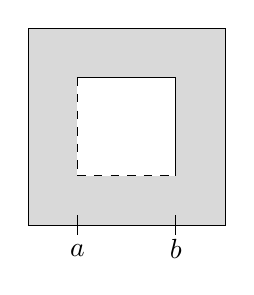
\begin{tikzpicture}[xscale=2.5, yscale=2.5]
		\draw[fill=gray!30] (0,0) rectangle (1,1);
		\draw[fill=white!30,draw=none] (0.25,0.25) rectangle (0.75,0.75);
		\draw (0.25,0.75) -- (0.75,0.75);
		\draw (0.25,0.75) -- (0.75,0.75);
		\draw (0.75,0.75) -- (0.75,0.25);
		\draw[dashed] (0.25,0.75) -- (0.25,0.25);
		\draw[dashed] (0.25,0.25) -- (0.75,0.25);
		\draw (0.25,-0.05) -- (0.25,0.05);
		\draw (0.75,-0.05) -- (0.75,0.05);
		\node[below] at (0.25,-0.05) {$a$};
		\node[below] at (0.75,-0.02) {$b$};
	\end{tikzpicture}\\
	\includegraphics[scale=0.41]{exnegdisc2}
	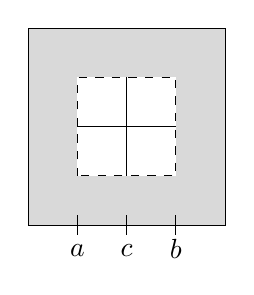
\begin{tikzpicture}[xscale=2.5, yscale=2.5]
		\draw[fill=gray!30] (0,0) rectangle (1,1);
		\draw[fill=white!30,dashed] (0.25,0.25) rectangle (0.75,0.75);
		\draw (0.5,0.25) -- (0.5,0.75);
		\draw (0.25,0.5) -- (0.75,0.5);
		\draw (0.25,-0.05) -- (0.25,0.05);
		\draw (0.5,-0.05) -- (0.5,0.05);
		\draw (0.75,-0.05) -- (0.75,0.05);
		\node[below] at (0.25,-0.05) {$a$};
		\node[below] at (0.5,-0.05) {$c$};
		\node[below] at (0.75,-0.02) {$b$};
	\end{tikzpicture}
	\caption{Two graphical examples of a fuzzy negation with one point of discontinuity and the corresponding region $(\Ran N \times [0,1])\cup (([0,1] \setminus \Ran N) \times \Ran N)$ in gray.}\label{fig:cases_discontinuities}
\end{figure}

\begin{remark}\label{remark:casesRanN}
	 Let $x_0 \in [0,1]$ be the single point of discontinuity of a fuzzy negation $N$. Let us compute all the possible values of $\Ran N$ depending of the discontinuity $x_0$ (knowing that it is of the first kind):
	\begin{enumerate}[label=\arabic*)]
		\item If $0=N(x_0^+)=N(x_0)<N(x_0^-)=1$ then 
		$$\Ran N = \{0\} \cup \{1\}.$$
		\item If $0=N(x_0^+)=N(x_0)<N(x_0^-)<1$ and $\exists x \in [0,1]$ such that $N(x)=N(x_0^-)$ then
		$$\Ran N = \{0\} \cup [N(x_0^-),1].$$
		\item If $0=N(x_0^+)=N(x_0)<N(x_0^-)<1$ and $\nexists x \in [0,1]$ such that $N(x)=N(x_0^-)$ then
		$$\Ran N = \{0\} \cup (N(x_0^-),1].$$
		\item If $0=N(x_0^+)<N(x_0)<N(x_0^-)=1$ then
		$$\Ran N = \{0\} \cup \{N(x_0)\} \cup \{1\}.$$
		\item If $0=N(x_0^+)<N(x_0)<N(x_0^-)<1$ and $\exists x \in [0,1]$ such that $N(x)=N(x_0^-)$ then
		$$\Ran N = \{0\} \cup \{N(x_0)\} \cup [N(x_0^-),1].$$
		\item If $0=N(x_0^+)<N(x_0)<N(x_0^-)<1$ and $\nexists x \in [0,1]$ such that $N(x)=N(x_0^-)$ then
		$$\Ran N = \{0\} \cup \{N(x_0)\} \cup (N(x_0^-),1].$$
		\item If $0=N(x_0^+)<N(x_0)=N(x_0^-)=1$ then
		$$\Ran N = \{0\} \cup \{1\}.$$
		\item If $0=N(x_0^+)<N(x_0)=N(x_0^-)<1$  then
		$$\Ran N = \{0\} \cup [N(x_0),1].$$
		\item If $0<N(x_0^+)=N(x_0)<N(x_0^-)=1$ then 
		$$\Ran N = [0,N(x_0)] \cup \{1\}.$$
		\item If $0<N(x_0^+)=N(x_0)<N(x_0^-)<1$ and $\exists x \in [0,1]$ such that $N(x)=N(x_0^-)$ then
		$$\Ran N = [0,N(x_0)] \cup [N(x_0^-),1].$$
		\item If $0<N(x_0^+)=N(x_0)<N(x_0^-)<1$ and $\nexists x \in [0,1]$ such that $N(x)=N(x_0^-)$ then
		$$\Ran N = [0,N(x_0)] \cup (N(x_0^-),1].$$
		\item If $0<N(x_0^+)<N(x_0)=N(x_0^-)=1$ and $\exists x \in [0,1]$ such that $N(x)=N(x_0^+)$ then
		$$\Ran N = [0,N(x_0^+)] \cup \{1\}.$$
		\item If $0<N(x_0^+)<N(x_0)=N(x_0^-)=1$ and $\nexists x \in [0,1]$ such that $N(x)=N(x_0^+)$ then
		$$\Ran N = [0,N(x_0^+)) \cup \{1\}.$$
		\item If $0<N(x_0^+)<N(x_0)=N(x_0^-)<1$ and $\exists x \in [0,1]$ such that $N(x)=N(x_0^+)$ then
		$$\Ran N = [0,N(x_0^+)] \cup [N(x_0),1].$$
		\item If $0<N(x_0^+)<N(x_0)=N(x_0^-)<1$ and $\nexists x \in [0,1]$ such that $N(x)=N(x_0^+)$ then
		$$\Ran N = [0,N(x_0^+)) \cup [N(x_0),1].$$
		\item If $0<N(x_0^+)<N(x_0)<N(x_0^-)=1$ and $\exists x \in [0,1]$ such that $N(x)=N(x_0^+)$ then
		$$\Ran N =[0,N(x_0^+)] \cup \{N(x_0)\} \cup \{1\}.$$
		\item If $0<N(x_0^+)<N(x_0)<N(x_0^-)=1$ and $\nexists x \in [0,1]$ such that $N(x)=N(x_0^+)$ then
		$$\Ran N =[0,N(x_0^+)) \cup \{N(x_0)\} \cup \{1\}.$$
		\item If $0<N(x_0^+)<N(x_0)<N(x_0^-)<1$, $\exists x \in [0,1]$ such that $N(x)=N(x_0^+)$ and $\exists x \in [0,1]$ such that $N(x)=N(x_0^-)$ then
		$$\Ran N =[0,N(x_0^+)] \cup \{N(x_0)\} \cup [N(x_0^-),1].$$
		\item If $0<N(x_0^+)<N(x_0)<N(x_0^-)<1$, $\exists x \in [0,1]$ such that $N(x)=N(x_0^+)$ and $\nexists x \in [0,1]$ such that $N(x)=N(x_0^-)$ then
		$$\Ran N =[0,N(x_0^+)] \cup \{N(x_0)\} \cup (N(x_0^-),1].$$
		\item If $0<N(x_0^+)<N(x_0)<N(x_0^-)<1$, $\nexists x \in [0,1]$ such that $N(x)=N(x_0^+)$ and $\exists x \in [0,1]$ such that $N(x)=N(x_0^-)$ then
		$$\Ran N =[0,N(x_0^+)) \cup \{N(x_0)\} \cup [N(x_0^-),1].$$
		\item If $0<N(x_0^+)<N(x_0)<N(x_0^-)<1$, $\nexists x \in [0,1]$ such that $N(x)=N(x_0^+)$ and $\nexists x \in [0,1]$ such that $N(x)=N(x_0^-)$ then
		$$\Ran N =[0,N(x_0^+)) \cup \{N(x_0)\} \cup (N(x_0^-),1].$$
	\end{enumerate}	
	Therefore, there are 21 possibilities for $\Ran N$. However, we are only interested in the structure of $\Ran N$ and we have that $1) \equiv 7)$, $2) \equiv 8)$, $10) \equiv 14)$ and $9) \equiv 12)$. In conclusion, we have the following 17 structures of $\Ran N$ where $0<a<c<b<1$:	
	$$
	\{0\} \cup \{1\}, \quad \{0\} \cup [b,1], \quad \{0\} \cup (b,1], \quad \{0\} \cup \{c\} \cup \{1\}, \quad \{0\} \cup \{c\} \cup [b,1],
	$$
	$$ 
	\quad \{0\} \cup \{c\} \cup (b,1], \quad [0,a] \cup \{1\}, \quad [0,a] \cup [b,1], \quad [0,a] \cup (b,1], \quad  [0,a) \cup \{1\}, 
	$$
	$$ 
	[0,a) \cup [b,1], \quad [0,a] \cup \{c\} \cup \{1\}, \quad [0,a) \cup \{c\} \cup \{1\}, \quad [0,a] \cup \{c\} \cup [b,1],
	$$
	$$[0,a] \cup \{c\} \cup (b,1], \quad [0,a) \cup \{c\} \cup [b,1], \quad [0,a) \cup \{c\} \cup (b,1].$$
\end{remark}
However, if we focus only on the continuous completions of $\SIN$ then we can take the first straightforward step of extending it to the boundaries of its domain by taking limits, i.e., if $B=(\Ran N \times [0,1]) \cup (([0,1]\setminus \Ran N) \times \Ran N)$ and $\overline{B}$ is the closure of $B$ we can define the function $\overline{S}_{I,N_I}: \overline{B} \to [0,1]$ as follows
$$
\overline{S}_{I,N_I}(x,y) =
\left\{ \begin{array}{ll}
	S_{I,N_I}(x,y) &   \text{if }   (x,y) \in B, \\
	\displaystyle \lim_{(x^*,y^*) \to (x,y)} S_{I,N_I}(x^*,y^*) &   \text{if }   (x,y) \in \overline{B} \setminus B.
\end{array} \right.
$$
It is clear that any continuous completion of $S_{I,N_I}$ must also coincide with $\overline{S}_{I,N_I}$ in $\overline{B} \setminus B$.
Therefore, in the cases obtained in Remark \ref{remark:casesRanN}, if $\Ran N$ contains some half-open interval we can complete that value using the continuity. Thus, we only have to consider the 8 following structures of  $\Ran N$
$$\{0\} \cup \{1\}, \quad \quad \{0\} \cup [b,1], \quad \{0\} \cup \{c\} \cup \{1\}, \quad \{0\} \cup \{c\} \cup [b,1], \quad [0,a] \cup \{1\}$$
$$[0,a] \cup [b,1], \quad [0,a] \cup \{c\} \cup \{1\}, \quad [0,a] \cup \{c\} \cup [b,1].$$
In this situation, these cases can be gathered in the eight subregions of $[0,1]^2$ collected in Figure \ref{fig:regions}. The correspondence between these regions and the cases in Remark \ref{remark:casesRanN} is given in Table \ref{table:correspondence_figures}.

\begin{table}[H]
	\centering
	\begin{tabular}{|c|c|}
		\hline
		\textbf{Region} & \textbf{Case} \\ \hline
		\textbf{$A_1$}     & 10, 11, 14, 15   \\ \hline
		\textbf{$A_2$}     & 9, 12, 13 \\ \hline
		\textbf{$A_3$}     & 2, 3, 8 \\ \hline
		\textbf{$A_4$}     & 1, 7 \\ \hline
		\textbf{$A_5$}     & 18, 19, 20, 21 \\ \hline
		\textbf{$A_6$}     & 16, 17 \\ \hline
		\textbf{$A_7$}     & 5, 6\\ \hline
		\textbf{$A_8$}     & 4 \\ \hline
	\end{tabular}
	\caption{Correspondence between the regions in Figure \ref{fig:regions} and the cases in Remark \ref{remark:casesRanN}.}
	\label{table:correspondence_figures}
\end{table}

\begin{figure}[t!]
	\centering
	\begin{subfigure}{.2\textwidth}
		\centering
		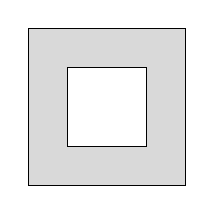
\begin{tikzpicture}[xscale=2, yscale=2]
			\draw[fill=gray!30] (0,0) rectangle (1,1);
			\draw[fill=white!30] (0.25,0.25) rectangle (0.75,0.75);
		\end{tikzpicture}
		\caption*{Region 1:\\
			 $A_1=[0,1]^2 \setminus (a,b)^2$ with $0<a<b<1$.}
	\end{subfigure}\hspace{0.5cm}
	\begin{subfigure}{.2\textwidth}
		\centering
		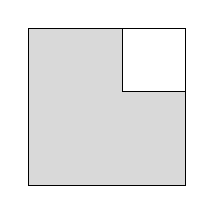
\begin{tikzpicture}[xscale=2, yscale=2]
			\draw[fill=gray!30] (0,0) rectangle (1,1);
			\draw[fill=white!30] (0.6,0.6) rectangle (1,1);
		\end{tikzpicture}
		\caption*{Region 2:\\
			 $A_2=[0,1]^2 \setminus (a,1)^2$ with $0<a<1$.}
	\end{subfigure}\hspace{0.5cm}
	\begin{subfigure}{.2\textwidth}
		\centering
		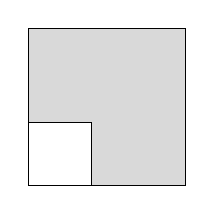
\begin{tikzpicture}[xscale=2, yscale=2]
			\draw[fill=gray!30] (0,0) rectangle (1,1);
			\draw[fill=white!30] (0,0) rectangle (0.4,0.4);
		\end{tikzpicture}
		\caption*{Region 3:\\
			 $A_3=[0,1]^2 \setminus (0,a)^2$ with $0<a<1$.}
	\end{subfigure}\hspace{0.5cm}
	\begin{subfigure}{.2\textwidth}
		\centering
		\begin{tikzpicture}[xscale=2, yscale=2]
			\draw (0,0) rectangle (1,1);
		\end{tikzpicture}
		\caption*{Region 4:\\
			 $A_4=[0,1]^2 \setminus (0,1)^2$. \\ \hspace{0.5cm} }
	\end{subfigure}\vspace{0.5cm}
	\begin{subfigure}{.2\textwidth}
		\centering
		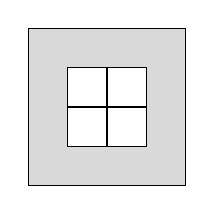
\begin{tikzpicture}[xscale=2, yscale=2]
			\draw[fill=gray!30] (0,0) rectangle (1,1);
			\draw[fill=white!30] (0.25,0.25) rectangle (0.75,0.75);
			\draw (0.25,0.5) -- (0.75,0.5);
			\draw (0.5,0.25) -- (0.5,0.75);
		\end{tikzpicture}
		\caption*{Region 5:\\
			 $A_5=([0,1]^2 \setminus (a,b)^2) \cup ([0,1] \times \{c\}) \cup (\{c\} \times [0,1])$ with $0<a<c<b<1$.}
	\end{subfigure}\hspace{0.5cm}
	\begin{subfigure}{.2\textwidth}
		\centering
		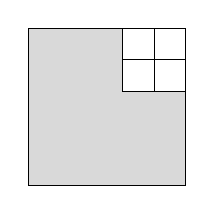
\begin{tikzpicture}[xscale=2, yscale=2]
			\draw[fill=gray!30] (0,0) rectangle (1,1);
			\draw[fill=white!30] (0.6,0.6) rectangle (1,1);
			\draw (0.6,0.8) -- (1,0.8);
			\draw (0.8,0.6) -- (0.8,1);
		\end{tikzpicture}
		\caption*{Region 6:\\
			 $A_6=([0,1]^2 \setminus (a,1)^2) \cup ([0,1] \times \{c\}) \cup (\{c\} \times [0,1])$ with $0<a<c<1$.}
	\end{subfigure}\hspace{0.5cm}
	\begin{subfigure}{.2\textwidth}
		\centering
		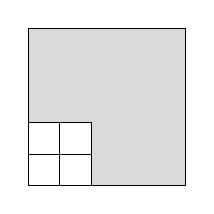
\begin{tikzpicture}[xscale=2, yscale=2]
			\draw[fill=gray!30] (0,0) rectangle (1,1);
			\draw[fill=white!30] (0,0) rectangle (0.4,0.4);
			\draw (0.4,0.2) -- (0,0.2);
			\draw (0.2,0.4) -- (0.2,0);
		\end{tikzpicture}
		\caption*{Region 7:\\
			 $A_7=([0,1]^2 \setminus (0,a)^2) \cup ([0,1] \times \{c\}) \cup (\{c\} \times [0,1])$ with $0<c<a<1$.}
	\end{subfigure}\hspace{0.5cm}
	\begin{subfigure}{.2\textwidth}
		\centering
		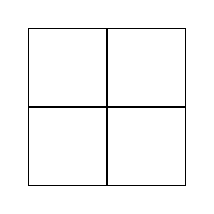
\begin{tikzpicture}[xscale=2, yscale=2]
			\draw (0,0) rectangle (1,1);
			\draw (0,0.5) -- (1,0.5);
			\draw (0.5,0) -- (0.5,1);
		\end{tikzpicture}
		\caption*{Region 8:\\
			 $A_8=([0,1]^2 \setminus (0,1)^2) \cup ([0,1] \times \{c\}) \cup (\{c\} \times [0,1])$ with $0<c<1$.\\
		 \hspace{0.5cm}}
	\end{subfigure}
	\caption{Regions (in gray) where we can uniquely determine the t-conorm S of an $(S,N)$-implication $I$ if we assume that the corresponding t-conorm is continuous and the negation has only one point of discontinuity.}
	\label{fig:regions}
\end{figure}

\pagebreak

If $N$ has more than one point of discontinuity the complexity of the region and the number of cases escalates rapidly. For instance, we have a particular case in Figure \ref{fig:example-threediscpoints} with three points of discontinuity.

\begin{figure}[t]
		\centering
\resizebox{0.68\textwidth}{!}{% 
	\tikzset{every picture/.style={line width=0.75pt}} %set default line width to 0.75pt        
	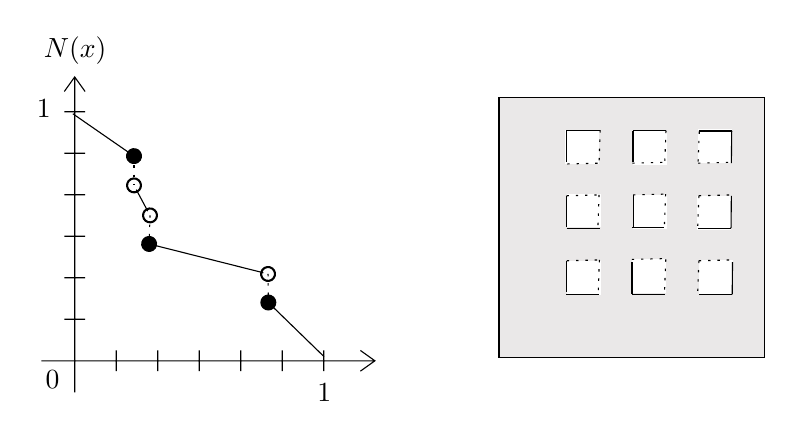
\begin{tikzpicture}[x=0.75pt,y=0.75pt,yscale=-1,xscale=1]
		%uncomment if require: \path (0,190); %set diagram left start at 0, and has height of 190
		
		%Shape: Rectangle [id:dp8958759845179514] 
		\draw  [draw opacity=0][fill={rgb, 255:red, 223; green, 221; blue, 221 }  ,fill opacity=0.67 ] (462.35,35.35) -- (334.32,35.35) -- (334.32,160.35) -- (462.35,160.35) -- cycle ;
		%Shape: Square [id:dp704858515624964] 
		\draw  [draw opacity=0][fill={rgb, 255:red, 255; green, 255; blue, 255 }  ,fill opacity=1 ] (430.8,113.62) -- (447.17,113.62) -- (447.17,129.98) -- (430.8,129.98) -- cycle ;
		%Shape: Square [id:dp3394861740721993] 
		\draw  [draw opacity=0][fill={rgb, 255:red, 255; green, 255; blue, 255 }  ,fill opacity=1 ] (398.34,113.16) -- (414.7,113.16) -- (414.7,129.52) -- (398.34,129.52) -- cycle ;
		%Shape: Square [id:dp07115105450204218] 
		\draw  [draw opacity=0][fill={rgb, 255:red, 255; green, 255; blue, 255 }  ,fill opacity=1 ] (367.04,113.79) -- (383.41,113.79) -- (383.41,130.15) -- (367.04,130.15) -- cycle ;
		%Shape: Square [id:dp5889504022793111] 
		\draw  [draw opacity=0][fill={rgb, 255:red, 255; green, 255; blue, 255 }  ,fill opacity=1 ] (429.91,82.58) -- (446.27,82.58) -- (446.27,98.95) -- (429.91,98.95) -- cycle ;
		%Shape: Square [id:dp9478064764482701] 
		\draw  [draw opacity=0][fill={rgb, 255:red, 255; green, 255; blue, 255 }  ,fill opacity=1 ] (398.96,82.07) -- (415.33,82.07) -- (415.33,98.44) -- (398.96,98.44) -- cycle ;
		%Shape: Square [id:dp09170108116485642] 
		\draw  [draw opacity=0][fill={rgb, 255:red, 255; green, 255; blue, 255 }  ,fill opacity=1 ] (366.88,81.41) -- (383.24,81.41) -- (383.24,97.77) -- (366.88,97.77) -- cycle ;
		%Shape: Square [id:dp1848415453306116] 
		\draw  [draw opacity=0][fill={rgb, 255:red, 255; green, 255; blue, 255 }  ,fill opacity=1 ] (430.24,50.4) -- (446.61,50.4) -- (446.61,66.77) -- (430.24,66.77) -- cycle ;
		%Shape: Square [id:dp12559727997608827] 
		\draw  [draw opacity=0][fill={rgb, 255:red, 255; green, 255; blue, 255 }  ,fill opacity=1 ] (398.9,51.14) -- (415.27,51.14) -- (415.27,67.51) -- (398.9,67.51) -- cycle ;
		%Shape: Square [id:dp3574132570359847] 
		\draw  [draw opacity=0][fill={rgb, 255:red, 255; green, 255; blue, 255 }  ,fill opacity=1 ] (366.15,50.8) -- (382.52,50.8) -- (382.52,67.16) -- (366.15,67.16) -- cycle ;
		%Shape: Axis 2D [id:dp05469933203577182] 
		\draw  (113.83,162) -- (274.54,162)(129.9,25.24) -- (129.9,177.19) (267.54,157) -- (274.54,162) -- (267.54,167) (124.9,32.24) -- (129.9,25.24) -- (134.9,32.24) (149.9,157) -- (149.9,167)(169.9,157) -- (169.9,167)(189.9,157) -- (189.9,167)(209.9,157) -- (209.9,167)(229.9,157) -- (229.9,167)(249.9,157) -- (249.9,167)(124.9,142) -- (134.9,142)(124.9,122) -- (134.9,122)(124.9,102) -- (134.9,102)(124.9,82) -- (134.9,82)(124.9,62) -- (134.9,62)(124.9,42) -- (134.9,42) ;
		\draw   ;
		%Straight Lines [id:da9494482773914164] 
		\draw    (129,42.97) -- (158.47,63.38) ;
		\draw [shift={(158.47,63.38)}, rotate = 34.71] [color={rgb, 255:red, 0; green, 0; blue, 0 }  ][fill={rgb, 255:red, 0; green, 0; blue, 0 }  ][line width=0.75]      (0, 0) circle [x radius= 3.35, y radius= 3.35]   ;
		%Straight Lines [id:da7803642319425699] 
		\draw    (159.58,79.56) -- (165.08,89.87) ;
		\draw [shift={(166.18,91.95)}, rotate = 61.94] [color={rgb, 255:red, 0; green, 0; blue, 0 }  ][line width=0.75]      (0, 0) circle [x radius= 3.35, y radius= 3.35]   ;
		\draw [shift={(158.47,77.49)}, rotate = 61.94] [color={rgb, 255:red, 0; green, 0; blue, 0 }  ][line width=0.75]      (0, 0) circle [x radius= 3.35, y radius= 3.35]   ;
		%Straight Lines [id:da6858543881076353] 
		\draw    (165.75,105.7) -- (220.77,119.58) ;
		\draw [shift={(223.05,120.16)}, rotate = 14.16] [color={rgb, 255:red, 0; green, 0; blue, 0 }  ][line width=0.75]      (0, 0) circle [x radius= 3.35, y radius= 3.35]   ;
		\draw [shift={(165.75,105.7)}, rotate = 14.16] [color={rgb, 255:red, 0; green, 0; blue, 0 }  ][fill={rgb, 255:red, 0; green, 0; blue, 0 }  ][line width=0.75]      (0, 0) circle [x radius= 3.35, y radius= 3.35]   ;
		%Straight Lines [id:da999883126310517] 
		\draw    (223.19,133.91) -- (250,159.97) ;
		\draw [shift={(223.19,133.91)}, rotate = 44.2] [color={rgb, 255:red, 0; green, 0; blue, 0 }  ][fill={rgb, 255:red, 0; green, 0; blue, 0 }  ][line width=0.75]      (0, 0) circle [x radius= 3.35, y radius= 3.35]   ;
		%Straight Lines [id:da7075761867262242] 
		\draw    (446.44,51.26) -- (446.28,66.77) ;
		%Straight Lines [id:da22472766824598267] 
		\draw    (366.63,50.89) -- (383.08,50.89) ;
		%Straight Lines [id:da5176694357488605] 
		\draw  [dash pattern={on 0.84pt off 2.51pt}]  (367.28,67.16) -- (382.92,66.77) ;
		%Straight Lines [id:da1695213907167461] 
		\draw  [dash pattern={on 0.84pt off 2.51pt}]  (398.56,66.77) -- (414.2,66.38) ;
		%Straight Lines [id:da5270356130997884] 
		\draw  [dash pattern={on 0.84pt off 2.51pt}]  (430.24,66.77) -- (445.88,66.38) ;
		%Straight Lines [id:da5217089839295574] 
		\draw  [dash pattern={on 0.84pt off 2.51pt}]  (414.78,51.14) -- (414.2,66.38) ;
		%Straight Lines [id:da1609691578490935] 
		\draw  [dash pattern={on 0.84pt off 2.51pt}]  (383.08,50.89) -- (382.52,67.16) ;
		%Straight Lines [id:da4103549447439565] 
		\draw  [dash pattern={on 0.84pt off 2.51pt}]  (366.88,82.47) -- (382.52,82.07) ;
		%Straight Lines [id:da8017335594741635] 
		\draw  [dash pattern={on 0.84pt off 2.51pt}]  (398.96,82.07) -- (414.6,81.68) ;
		%Straight Lines [id:da5763126871206965] 
		\draw  [dash pattern={on 0.84pt off 2.51pt}]  (430.64,82.47) -- (446.28,82.07) ;
		%Straight Lines [id:da6968359857940798] 
		\draw    (367.04,98.2) -- (382.92,98.2) ;
		%Straight Lines [id:da5592376807486388] 
		\draw    (398.34,97.85) -- (413.98,97.85) ;
		%Straight Lines [id:da6032310310486315] 
		\draw  [dash pattern={on 0.84pt off 2.51pt}]  (367.04,113.79) -- (382.68,113.4) ;
		%Straight Lines [id:da6615678947926249] 
		\draw  [dash pattern={on 0.84pt off 2.51pt}]  (398.34,113.16) -- (413.98,112.76) ;
		%Straight Lines [id:da055113940110814275] 
		\draw  [dash pattern={on 0.84pt off 2.51pt}]  (430.64,113.79) -- (446.28,113.4) ;
		%Straight Lines [id:da5917572007643113] 
		\draw    (366.63,129.98) -- (382.51,129.98) ;
		%Straight Lines [id:da7074071376091156] 
		\draw    (398.41,129.87) -- (414.29,129.87) ;
		%Straight Lines [id:da48375646476531786] 
		\draw    (430.8,129.98) -- (446.68,129.98) ;
		%Straight Lines [id:da6015720762353796] 
		\draw    (430.24,98.09) -- (446.12,98.09) ;
		%Straight Lines [id:da13347193784387423] 
		\draw    (398.9,51.14) -- (414.78,51.14) ;
		%Straight Lines [id:da05235501625594696] 
		\draw    (430.56,51.26) -- (446.44,51.26) ;
		%Straight Lines [id:da2423446258877633] 
		\draw    (398.41,114.57) -- (398.41,129.87) ;
		%Straight Lines [id:da8488705740850397] 
		\draw    (398.96,82.07) -- (398.96,97.38) ;
		%Straight Lines [id:da4183161634531327] 
		\draw    (398.9,51.14) -- (398.9,66.45) ;
		%Straight Lines [id:da4910825267117853] 
		\draw    (366.63,50.89) -- (366.63,66.2) ;
		%Straight Lines [id:da2545284440450135] 
		\draw  [dash pattern={on 0.84pt off 2.51pt}]  (382.52,82.07) -- (381.96,98.34) ;
		%Straight Lines [id:da0780495625881712] 
		\draw  [dash pattern={on 0.84pt off 2.51pt}]  (382.68,113.4) -- (382.12,129.66) ;
		%Straight Lines [id:da07867768731348024] 
		\draw    (366.88,82.47) -- (366.88,97.77) ;
		%Straight Lines [id:da20763244618197052] 
		\draw    (367.04,113.79) -- (367.04,129.09) ;
		%Straight Lines [id:da8032904773267526] 
		\draw  [dash pattern={on 0.84pt off 2.51pt}]  (414.6,81.68) -- (414.02,96.92) ;
		%Straight Lines [id:da7446171371781336] 
		\draw  [dash pattern={on 0.84pt off 2.51pt}]  (414.67,113.16) -- (414.09,128.39) ;
		%Straight Lines [id:da22928253260249987] 
		\draw  [dash pattern={on 0.84pt off 2.51pt}]  (430.82,51.53) -- (430.24,66.77) ;
		%Straight Lines [id:da8395358709511287] 
		\draw  [dash pattern={on 0.84pt off 2.51pt}]  (430.64,82.47) -- (430.06,97.7) ;
		%Straight Lines [id:da2513131704470868] 
		\draw  [dash pattern={on 0.84pt off 2.51pt}]  (430.64,113.79) -- (430.06,129.03) ;
		%Straight Lines [id:da7253223876817636] 
		\draw    (446.27,82.58) -- (446.12,98.09) ;
		%Straight Lines [id:da9903820773786822] 
		\draw    (446.84,114.47) -- (446.68,129.98) ;
		%Straight Lines [id:da27662027020346946] 
		\draw  [dash pattern={on 0.84pt off 2.51pt}]  (158.47,63.38) -- (158.47,77.49) ;
		%Straight Lines [id:da8278673182766836] 
		\draw  [dash pattern={on 0.84pt off 2.51pt}]  (166.18,91.95) -- (165.75,105.7) ;
		%Straight Lines [id:da1082595058417537] 
		\draw  [dash pattern={on 0.84pt off 2.51pt}]  (223.05,120.16) -- (223.19,133.91) ;
		%Shape: Rectangle [id:dp6709977120749835] 
		\draw   (334.32,35.35) -- (462.35,35.35) -- (462.35,160.35) -- (334.32,160.35) -- cycle ;
		
		% Text Node
		\draw (119.21,171.05) node    {$0$};
		% Text Node
		\draw (250.19,177.46) node    {$1$};
		% Text Node
		\draw (130.11,12.61) node    {$N( x)$};
		% Text Node
		\draw (115.02,40.34) node    {$1$};
		
		
	\end{tikzpicture}
}
	\caption{A graphical example of a fuzzy negation with three points of discontinuity and  the corresponding region $(\Ran N \times [0,1]) \cup (([0,1] \setminus \Ran N) \times \Ran N)$ in gray.}\label{fig:example-threediscpoints}
\end{figure}

Due to these facts, as the first step for solving the problem of completing a pre-t-conorm known in $(\Ran N \times [0,1]) \cup (([0,1] \setminus \Ran N) \times \Ran N)$ to a t-conorm we assume two \textbf{sensible assumptions} that simplify the problem: $N$ has only one point of discontinuity and $S$ is a continuous t-conorm. Thus, we are interested in the continuous completions of pre-t-conorms defined on one of the regions of Figure \ref{fig:regions}.


\subsection{Duality between the completion problem for pre-t-conorms and pre-t-norms}\label{subsec:dualitypretnorms/conorms}
Notice that, as a matter of fact, we are interested in the completion to a t-conorm of functions defined on one of the regions in Figure \ref{fig:regions}. However, in the next section we point out that all the existing literature on this topic deals with the problem of finding the continuous completions of t-norms. Therefore, in order to be consistent with the literature and to apply directly the results already known to our particular problems, we will also maintain this perspective. For this reason, we provide the definition of pre-t-norm and some related concepts which are analogous to the case of pre-t-conorms.
\begin{definition}\label{def:completiont-norm} Let $T_A:A \to [0,1]$ be a function defined on $A \subseteq [0,1]^2$. $T_A$ can be \emph{completed} to a t-norm if there exists a t-norm $T:[0,1]^2 \to [0,1]$ such that $T_A(x,y)=T(x,y)$ for all $(x,y) \in A$. In this case, $T$ is said to be a completion of $T_A$. If $T$ is a continuous t-norm we say that it is a \emph{continuous completion}.
\end{definition}
The definition of pre-t-norm ensures that this function satisfies the properties of a t-norm on a subregion of $[0,1]^2$.
\begin{definition}\label{def:TA} A function $T_A:A \to [0,1]$ is called a \emph{pre-t-norm} in $A \subseteq [0,1]^2$ if it satisfies the following conditions:
	$$T_A(x,y)=T_A(y,x), \quad \text{for all } (x,y), (y,x) \in A,$$
	$$T_A(x,T_A(y,z))=T_A(T_A(x,y),z), \quad \text{for all } (y,z), (x,T_A(y,z)), (x,y), (T_A(x,y),z)\in A,$$
	$$T_A(x,y) \leq T_A(x,z), \quad \text{for all } (x,y),(x,z) \in A \text{ such that } y \leq z,$$
	$$T_A(x,z) \leq T_A(y,z), \quad \text{for all } (x,z),(y,z) \in A \text{ such that } x \leq y,$$
	$$T_A(1,x)=x \quad \text{ for all } (1,x) \in A \text{ and } T_A(x,1)=x \quad \text{ for all } (x,1) \in A.$$
\end{definition}
\begin{proposition}
	Let $T_A:A \to [0,1]$ be a function defined on $A \subseteq [0,1]^2$. If $T_A$ can be completed to a t-norm $T$, then $T_A$ is a pre-t-norm.
\end{proposition}
Similarly to the case of t-norms, we define cancellative and conditionally cancellative pre-t-norms.
\begin{definition}\label{def:cancellative} Let $T_A:A \to [0,1]$  be a pre-t-norm defined on $A\subseteq [0,1]^2$, then $T_A$ is called:
	\begin{enumerate}[label=(\alph*)]
		\item \emph{cancellative} if $T_A(x,y)=T_A(x,z)$  implies $y=z$ for all $(x,y),(x,z) \in A$, $x>0$ and  $T_A(y,x)=T_A(z,x)$ implies $y=z$ for all $(y,x),(z,x) \in A$, $x>0$.
		\item \emph{conditionally cancellative} if $T_A(x,y)=T_A(x,z)>0$ implies $y=z$ for all $(x,y),(x,z) \in A$ and $T_A(y,x)=T_A(z,x)>0$ implies $y=z$ for all $(y,x),(z,x) \in A$.
	\end{enumerate}
\end{definition}
The following result points out that if $A$ contains the region $[0,1]^2 \setminus [0,1)^2$ then the pre-t-norm is  less or equal to the minimum.
\begin{proposition}\label{prop:pre-t-norm-minimum} Let $T_A: A \to [0,1]$ be a pre-t-norm defined on $A\subseteq [0,1]^2$ such that $[0,1]^2 \setminus [0,1)^2 \subseteq A$. Then, $T_A(x,y) \leq \min \{x,y\}$ for all $(x,y) \in A$.
\end{proposition}
\begin{proof}
	Let $(x,y) \in A$, we have
	$$T_A(x,y) \leq T_A(x,1) =x, \quad T_A(x,y) \leq T_A(1,y) =y,$$
	and then $T_A(x,y) \leq \min \{x,y\}$.
\end{proof}
The following proposition shows that for the case of pre-t-norms/pre-t-conorms there is a duality similar to the case of t-norms/t-conorms. However, it is clear that in our case the region were a pre-t-norm/pre-t-conorm is defined is affected by the corresponding transformation.
\pagebreak
\begin{proposition}\label{prop:duality:pretnormsconorms} The following statements hold:
	\begin{enumerate}[label=(\roman*)]
		\item If $S_A : A \to [0,1]$ with $A \subseteq [0,1]^2$ is a pre-t-conorm, then the function $T_B:B \to [0,1]$ defined as 
		$$T_B(x,y)=1-S_A(1-x,1-y), \quad (x,y) \in B,$$
		with $B=\{(x,y) \in [0,1]^2 \mid (1-x,1-y) \in A\}$ is a pre-t-norm. Moreover, if $S_A$ is continuous and cancellative (resp. conditionally cancellative but not cancellative) then $T_B$ is also continuous and cancellative (resp. conditionally cancellative but not cancellative). In this case, if $S$ is a completion of $S_A$, then the t-norm $T:[0,1]^2 \to [0,1]$ defined as
		$$T(x,y)=1-S(1-x,1-y), \quad (x,y) \in [0,1]^2,$$
		is a completion of $T_B$.
		\item If $T_A : A \to [0,1]$ with $A \subseteq [0,1]^2$ is a pre-t-norm, then the function $S_B:B \to [0,1]$ defined as 
		$$S_B(x,y)=1-T_A(1-x,1-y), \quad (x,y) \in B,$$
		with $B=\{(x,y) \in [0,1]^2 \mid (1-x,1-y) \in A\}$ is a pre-t-conorm. Moreover, if $T_A$ is continuous and cancellative (resp. conditionally cancellative but not cancellative) then $S_B$ is also continuous and cancellative (resp. conditionally cancellative but not cancellative). In this case, if $T$ is a completion of $T_A$, then the t-conorm $S:[0,1]^2 \to [0,1]$ defined as
		$$S(x,y)=1-T(1-x,1-y), \quad (x,y) \in [0,1]^2,$$
		is a completion of $S_B$.
	\end{enumerate}
\end{proposition}
\begin{proof} Let us prove only Point (i), since Point (ii) is analogous. Let $S_A : A \to [0,1]$ with $A \subseteq [0,1]^2$ be a pre-t-conorm, we define  the function $T_B:B \to [0,1]$ as
$$T_B(x,y)=1-S_A(1-x,1-y), \quad (x,y) \in B,$$
with $B=\{(x,y) \in [0,1]^2 \mid (1-x,1-y) \in A\}$. To see that $\TB$ is a pre-t-norm we have to check the four conditions in Definition \ref{def:TA}: \enlargethispage{20pt}
\begin{itemize}
	\item Let $(x,y),(y,x) \in B$, then $(1-x,1-y), (1-y,1-x) \in A$ and since $S_A$ is a pre-t-conorm
	$$T_B(x,y)=1-S_A(1-x,1-y)=1-S_A(1-y,1-x)=T_B(y,x).$$
	\item Let $(y,x),(x,T_B(y,z)),(x,y),(T_B(x,y),z) \in B$, then $(1-y,1-x),(1-x,1-T_B(y,z)),(1-x,1-y),(1-T_B(x,y),1-z) \in A$ and by definition of $T_B$ we have $(1-y,1-x),(1-x,S_A(1-y,1-z)),(1-x,1-y),(S_A(1-x,1-y),1-z) \in A$. Thus,  since $S_A$ is a pre-t-conorm
	\begin{eqnarray*}
	T_B(x,T_B(y,z)) & = & T_B(x,1-S_A(1-y,1-z)) = 1-S_A(1-x,S_A(1-y,1-z)) \\
	& = & 1-S_A(S_A(1-x,1-y),1-z)=T_B(1-S_A(1-x,1-y),z) \\
	& = & T_B(T_B(x,y),z).
	\end{eqnarray*}
	\item Let $(x,y),(y,z) \in B$ such that $x \leq y$, then $(1-x,1-y),(1-y,1-z) \in A$ and $1-x \geq 1-y$. Thus, since $S_A$ is a pre-t-conorm 
	$$T_B(x,z)=1-S_A(1-x,1-z) \leq 1-S_A(1-y,1-z)=T_B(y,z).$$
	\item Let $(x,1) \in B$, then $(1-x,0) \in A$ and since $S_A$ is a pre-t-conorm
	$$T_B(x,1)=1-S_A(1-x,0)=1-(1-x)=x.$$
\end{itemize}
Now, it is straightforward to see that since $S_A$ is continuous, then $T_B$ is also continuous. Let $S_A$ be a cancellative pre-t-conorm and consider $(x,y),(x,z) \in B$ with $x>0$, then $(1-x,1-y),(1-x,1-z) \in A$ with $1-x<1$, we have
\begin{eqnarray*}
T_B(x,y) = T_B(x,z) &\Rightarrow& 1-S_A(1-x,1-y)=1-S_A(1-x,1-z)\\
 &\Rightarrow& S_A(1-x,1-y)=S_A(1-x,1-z) 
\Rightarrow 1-y=1-z \\
& \Rightarrow & y=z.
\end{eqnarray*}
If $(y,x),(z,x) \in B$ with $x>0$ the proof is analogous. On the other hand, let $S_A$ be a conditionally cancellative but not cancellative pre-t-norm and consider $(x,y),(x,z) \in B$, then
\begin{eqnarray*}
	T_B(x,y) = T_B(x,z)>0 &\Rightarrow& 1-S_A(1-x,1-y)=1-S_A(1-x,1-z)>0\\
	&\Rightarrow& S_A(1-x,1-y)=S_A(1-x,1-z)<1
	\Rightarrow 1-y=1-z \\
	&\Rightarrow& y=z.
\end{eqnarray*}
If $(y,x),(z,x) \in B$ the proof is analogous. Finally, since $S_A$ is not cancellative there exists $(x,y) \in A$ with $x,y \not = 1$ such that $S_A(x,y)=1$. Then $(1-x,1-y) \in B$ with $1-x,1-y \not = 0$ and
$$T_B(1-x,1-y)=1-S_A(x,y)=1-1=0,$$
so we obtain that $T_B$ is not cancellative.
\end{proof}

In view of Proposition \ref{prop:duality:pretnormsconorms}, in order to prove that the problem of finding all the continuous completions of a pre-t-conorm defined on one of the regions in Figure \ref{fig:regions} is analogous to the case of pre-t-norms, we need to prove that if $A_i$ is one of the regions in Figure \ref{fig:regions} then $\tilde{A_i} = \{(x,y) \in [0,1]^2 \mid (1-x,1-y) \in A_i\}$ also corresponds to one of the regions in Figure \ref{fig:regions}. Indeed, this correspondence is pointed out in the following lemma.

\begin{lemma}\label{lemma:dualregions}
	Let $A_i$ be one of the regions in Figure \ref{fig:regions} and let $\tilde{A_i} = \{(x,y) \in [0,1]^2 \mid (1-x,1-y) \in A_i\}$. The following statements hold:
	\begin{itemize}
		\item If $A_i=A_1$ with $0<a<b<1$ then $\tilde{A_i}=A_1$ with $\tilde{a}=1-b$ and $\tilde{b}=1-a$.
		\item If $A_i=A_2$ with $a \in (0,1)$ then $\tilde{A_i}=A_3$ with $\tilde{a}=1-a$.
		\item If $A_i=A_3$ with $a \in (0,1)$ then $\tilde{A_i}=A_2$ with $\tilde{a}=1-a$.
		\item If $A_i=A_4$ then $\tilde{A_i}=A_4$.
		\item $A_i=A_5$ with $0<a<c<b<1$ then $\tilde{A_i}=A_5$ with $\tilde{a}=1-b$, $\tilde{c}=1-c$ and $\tilde{b}=1-a$.
		\item If $A_i=A_6$ with $0<a<c<1$ then $\tilde{A_i}=A_7$ with $\tilde{c}=1-c$ and $\tilde{a}=1-a$.
		\item If $A_i=A_7$ with $0<c<a<1$ then $\tilde{A_i}=A_7$ with $\tilde{a}=1-a$ and $\tilde{c}=1-c$.
		\item If $A_i=A_8$ with $0<c<1$ then $\tilde{A_i}=A_8$ with $\tilde{c}=1-c$.
	\end{itemize}
\end{lemma}
\begin{proof}
	Let us prove only the first point, since the other 7 are analogous. If $A_i=A_1$ with $0<a<b<1$ then
	\begin{eqnarray*}
	(x,y) \in \tilde{A_i} &\Leftrightarrow&(1-x,1-y) \in A_i \Leftrightarrow 1-x \in [0,a] \cup [b,1] \text{ or } 1-y \in [0,a] \cup [b,1] \\
	& \Leftrightarrow & x \in [1-a,1] \cup [0,1-b] \text{ or } y \in [1-a,1] \cup [0,1-b]\\
		& \Leftrightarrow & (x,y) \in A_1 \text{ with } \tilde{a}=1-b \text{ and } \tilde{b}=1-a.
	\end{eqnarray*} 
\end{proof}

In view of the duality of the two problems, in the following sections we focus on the problem of the completion of continuous pre-t-norms defined on one of the regions of Figure \ref{fig:regions}. 


\subsection{Related bibliography}\label{subsec:related_bibliography}

The problem of existence and uniqueness of continuous Archimedean t-norms, given their restriction to certain subsets of $[0,1]^2$ is a recurrent problem in the study of t-norms \cite{Alsina2006}. The problem consists on determining whether a function  $T_A$ on $A\subseteq [0,1]^2$, which is consistent with the conditions of t-norms, can be completed to a continuous t-norm $T$ (usually Archimedean) in the sense of Definition \ref{def:completiont-norm} and, if so, whether the completion is unique. Taking into account the representation theorem of continuous Archimedean t-norms, the problem is equivalent to the study of existence and uniqueness of additive generators, up to a positive multiplicative constant. That is to say, $T_A$ can be completed to $T$ if and only if there exists a continuous strictly decreasing function $t:[0,1] \to [0,+\infty]$ with $t(1)=0$ such that
$$T(x,y) = t^{(-1)}(t(x)+t(y)), \text{ for all  } x,y \in [0,1]^2, \text{ and }  T(x,y)=T_A(x,y), \text {for all  } (x,y) \in A.$$
Moreover, this completion is unique if and only if $t$ is unique up to a positive multiplicative constant. In this case, we say that $A$ is a \emph{set of uniqueness} of $T$.\\
Depending on the choices of $A$, the problem leads to solve different functional equations. From now on, we list all the results that we found related to this problem in the literature. We distinguish between three types of results. First, we enumerate the results that explicitly construct an additive generator $t$ of a completion of $T_A$.

\begin{enumerate}[label=(C-\arabic*)]
	\item If $A$ is a diagonal, the choices for the additive generator $t$ are solutions of Schröder equation. In this case, $A$ is not a set of uniqueness so a continuous completion is not unique \cite{Alsina2006,Kimberling1973,Mesiar1999}.
	\item If $A$ is a horizontal/vertical section, the choices for the additive generator $t$ are solutions of Abel's equation. In this case, $A$ is not a set of uniqueness so a continuous completion is not unique \cite{Alsina2006}.
	\item If $A$ is a level curve, i.e., $A$ is the graph of any strictly decreasing function $l:[z,1] \to [z,1]$ with $z \in [0,1)$ such that $l^{-1}=l$, the choices for the additive generator $t$ are solutions of the functional equation $t(x)+t(l(x))=1$. In this case, $A$ is not a set of uniqueness so a continuous completion is not unique \cite{Alsina2006}.
	\item If $A=[a,b]^2 \subsetneq [0,1]^2$ with $0 \leq a < b \leq 1$ the problem is solved in \cite{Mesiarova2017}. In this case, $A$ is not a set of uniqueness so a continuous completion is not unique.
\end{enumerate}
Second, we sum up the results that determine whether $A$ is a set of uniqueness. This type of results are specially useful to determine if a certain completion is unique. However, these results do not usually provide any information on the additive generator of the possible completion.
\begin{enumerate}[label=(SU-\arabic*)]
	\item $A=\bigtriangleup_{\varepsilon}$ where $\bigtriangleup_{\varepsilon}$ is the triangle with edges $(1-\varepsilon,0)$, $(1,0)$ and $(1,1)$, where $\varepsilon \in (0,1]$, is a set of uniqueness \cite{Kimberling1973,Klement2000}.
	\item If $A$ is the union of a level curve and the diagonal, then $A$ is a set of uniqueness \cite{Alsina2006}.
	\item In \cite{Darsow1983} the authors determine several sets of uniqueness formed by the diagonal and a certain piece of a horizontal section and a certain piece of the diagonal.
	\item In \cite{Bezivin1993} the authors determine various sets of uniqueness of a strict t-norm that involve the main diagonal and some additional information. For instance, one of them is when $A$ is the union of the two diagonals.
	\item In \cite{Jenei2005} the author determines a set of uniqueness of an Archimedean t-norm formed by a numerable number of segments.
\end{enumerate}
Finally, there are some results that highlight subregions of $[0,1]^2$ that are not sets of uniqueness, i.e., the values of a t-norm in that regions do not determine in a unique manner the rest of the values.
\begin{enumerate}[label=(NSU-\arabic*)]
	\item If $A$ is the union of a horizontal section and a level curve, then $A$ is not a set of uniqueness \cite{Alsina2006}.
	\item If $A$ is the union of two horizontal sections, then $A$ is not a set of uniqueness \cite{Alsina2006}.
	\item If $A=[0,1-\varepsilon]^2$ with $\varepsilon\in(0,1]$, then $A$ is not a set of uniqueness \cite{Alsina2006}. This result can also be obtained directly from (C-4).
\end{enumerate}
%\RFc{He d'explicar també que totes les completacions no son uniques per tant son conjunts de no unicitat. Com ho puc marcar al diagrama?}
In Figure \ref{fig:SurveyCompletions} a visual summary of all the mentioned results can be found.\\

\begin{figure}[t!]
		\centering
		\begin{subfigure}[t]{.2\textwidth} \centering
				\resizebox{\textwidth}{!}{%
				\begin{tikzpicture}[xscale=3, yscale=3]
					\node[above left,text=white] at (0.05,0.96) {$S$};
					\node[above right] at (0.95,0.95) {$C$};
					\draw [line width=0.4mm, forestgreen ] (0,0) -- (1,1);
					\draw (0,0) rectangle (1,1);
					\node[below] at (0.5,-0.1) {(C-1)};
				\end{tikzpicture}
			}
			%\caption*{(C-1)}
		\end{subfigure}\hspace{0.5cm}
		\begin{subfigure}[t]{.2\textwidth}\centering
			\resizebox{\textwidth}{!}{%
			\begin{tikzpicture}[xscale=3, yscale=3]
					\node[above left,text=white] at (0.05,0.96) {$S$};
					\node[above right] at (0.95,0.95) {$C$};
					\draw [line width=0.4mm, forestgreen ] (0,0.5) -- (1,0.5);
					\node[below] at (0.5,-0.1) {(C-2)};
					\draw (0,0) rectangle (1,1);
			\end{tikzpicture}
		}
		\end{subfigure}\hspace{0.5cm}
		\begin{subfigure}[t]{.2\textwidth}\centering
			\resizebox{\textwidth}{!}{%
			\begin{tikzpicture}[xscale=3, yscale=3]
				\node[above left,text=white] at (0.05,0.96) {$S$};
				\node[above right] at (0.95,0.95) {$C$};
				\draw [line width=0.4mm, forestgreen] plot [smooth, tension=1] coordinates { (0.5,1) (0.65,0.65) (1,0.5)};
				\node[below] at (0.5,-0.1) {(C-3)};
				\draw (0,0) rectangle (1,1);
			\end{tikzpicture}
			}
		\end{subfigure}\hspace{0.5cm}
		\begin{subfigure}[t]{.2\textwidth}\centering
			\resizebox{\textwidth}{!}{%
			\begin{tikzpicture}[xscale=3, yscale=3]
				\node[above left,text=white] at (0.05,0.96) {$S$};
				\node[above right] at (0.95,0.95) {$C$};
				\draw[fill=forestgreen!70] (0.25,0.25) rectangle (0.75,0.75);
				\node[below] at (0.5,-0.1) {(C-4)-1};
				\draw (0,0) rectangle (1,1);
			\end{tikzpicture}
		}
		\end{subfigure}\vspace{0.5cm}\\
		\begin{subfigure}[t]{.2\textwidth}\centering
			\resizebox{\textwidth}{!}{%
			\begin{tikzpicture}[xscale=3, yscale=3]
				\node[above left,text=white] at (0.05,0.96) {$S$};
				\node[above right] at (0.95,0.95) {$C$};
				\draw[fill=forestgreen!70] (0,0) rectangle (0.4,0.4);
				\node[below] at (0.5,-0.1) {(C-4)-2};
				\draw (0,0) rectangle (1,1);
			\end{tikzpicture}
		}
		\end{subfigure}\hspace{0.5cm}
		\begin{subfigure}{.2\textwidth}\centering
			\resizebox{\textwidth}{!}{%
			\begin{tikzpicture}[xscale=3, yscale=3]
				\node[above left,text=white] at (0.05,0.96) {$S$};
				\node[above right] at (0.95,0.95) {$C$};
				\draw[fill=forestgreen!70] (0.6,0.6) rectangle (1,1);
				\node[below] at (0.5,-0.1) {(C-4)-3};
				\draw (0,0) rectangle (1,1);
			\end{tikzpicture}
		}
		\end{subfigure}\hspace{0.5cm}
		\begin{subfigure}{.2\textwidth}\centering
			\resizebox{\textwidth}{!}{%
		\begin{tikzpicture}[xscale=3, yscale=3]
			\node[above left,text=white] at (0.05,0.96) {$S$};
			\node[above right,text=white] at (0.95,0.95) {$C$};
			\draw [line width=0.4mm, forestgreen] (0,0.4) -- (1,0.4);
			\draw [line width=0.4mm, forestgreen] plot [smooth, tension=1] coordinates { (0.5,1) (0.65,0.65) (1,0.5)};
			\node[below] at (0.5,-0.1) {(NSU-1)};
			\draw (0,0) rectangle (1,1);
		\end{tikzpicture}
	}
	\end{subfigure}\hspace{0.5cm}
	\begin{subfigure}{.2\textwidth}\centering
		\resizebox{\textwidth}{!}{%
		\begin{tikzpicture}[xscale=3, yscale=3]
			\node[above left,text=white] at (0.05,0.96) {$S$};
			\node[above right,text=white] at (0.95,0.95) {$C$};
			\draw [line width=0.4mm, forestgreen] (0,0.4) -- (1,0.4);
			\draw [line width=0.4mm, forestgreen] (0,0.7) -- (1,0.7);
			\node[below] at (0.5,-0.1) {(NSU-2)};
			\draw (0,0) rectangle (1,1);
		\end{tikzpicture}
		}
	\end{subfigure}\vspace{0.5cm}
	\begin{subfigure}{.2\textwidth}
		\centering
		\resizebox{\textwidth}{!}{%
		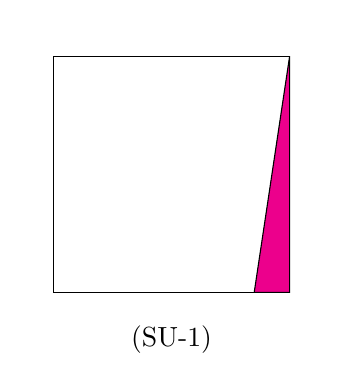
\begin{tikzpicture}[xscale=3, yscale=3]
			\node[above left,text=white] at (0.05,0.96) {$S$};
			\node[above right,text=white] at (0.95,0.95) {$C$};
			\draw[fill=magenta] (0.85,0) coordinate(A) -- (1,0) coordinate(B) -- (1,1) coordinate(C) -- cycle; 
			\node[below] at (0.5,-0.1) {(SU-1)};
			\draw (0,0) rectangle (1,1);
		\end{tikzpicture}
	}
	\end{subfigure}\hspace{0.5cm}
	\begin{subfigure}{.2\textwidth} \centering
		\resizebox{\textwidth}{!}{%
		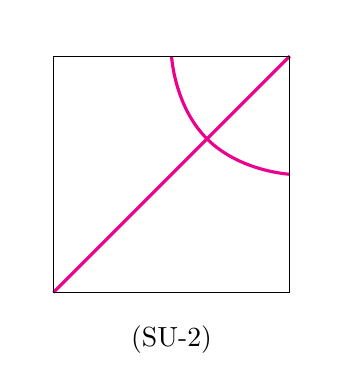
\begin{tikzpicture}[xscale=3, yscale=3]
				\node[above left,text=white] at (0.05,0.96) {$S$};
				\node[above right,text=white] at (0.95,0.95) {$C$};
				\draw [line width=0.4mm, magenta] (0,0) -- (1,1);
				\draw [line width=0.4mm, magenta] plot [smooth, tension=1] coordinates { (0.5,1) (0.65,0.65) (1,0.5)};
				\node[below] at (0.5,-0.1) {(SU-2)};
				\draw (0,0) rectangle (1,1);
			\end{tikzpicture}
		}
	\end{subfigure}\hspace{0.5cm}
	\begin{subfigure}{.2\textwidth}
		\centering
		\resizebox{\textwidth}{!}{%
		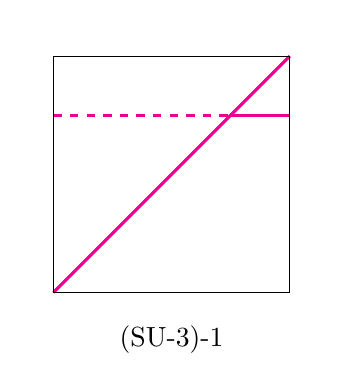
\begin{tikzpicture}[xscale=3, yscale=3]
				\draw [line width=0.4mm, magenta] (0,0) -- (1,1);
				\node[above left,text=white] at (0.05,0.96) {$S$};
				\node[above right,text=white] at (0.95,0.95) {$C$};
				\draw [line width=0.4mm, dashed, magenta] (0,0.75) -- (1,0.75);
				\draw [line width=0.4mm, magenta] (1,0.75) -- (0.75,0.75);
				\node[below] at (0.5,-0.1) {(SU-3)-1};
				\draw (0,0) rectangle (1,1);
			\end{tikzpicture}
		}
	\end{subfigure}\hspace{0.5cm}
	\begin{subfigure}{.2\textwidth}
		\centering
		\resizebox{\textwidth}{!}{%
		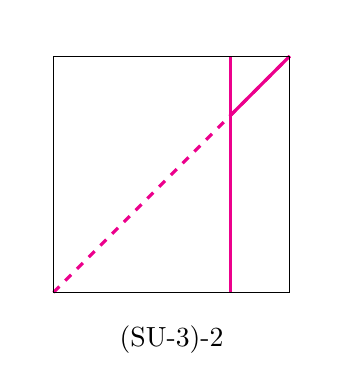
\begin{tikzpicture}[xscale=3, yscale=3]
			\node[above left,text=white] at (0.05,0.96) {$S$};
			\node[above right,text=white] at (0.95,0.95) {$C$};
			\draw [line width=0.4mm, dashed,magenta] (0,0) -- (1,1);
			\draw [line width=0.4mm, magenta] (0.75,0.75) -- (1,1);
			\draw [line width=0.4mm, magenta] (0.75,0) -- (0.75,1);
			\node[below] at (0.5,-0.1) {(SU-3)-2};
			\draw (0,0) rectangle (1,1);
		\end{tikzpicture}
	}
	\end{subfigure}\vspace{0.5cm}
	\begin{subfigure}{.2\textwidth}
		\centering
		\resizebox{\textwidth}{!}{%
		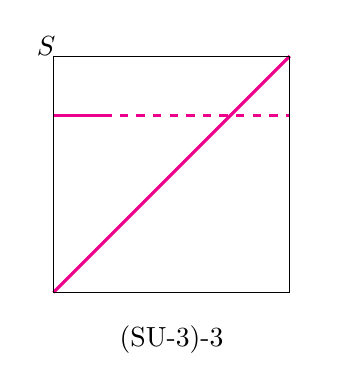
\begin{tikzpicture}[xscale=3, yscale=3]
			\node[above left] at (0.05,0.96) {$S$};
			\node[above right,text=white] at (0.95,0.95) {$C$};
			\draw [line width=0.4mm, magenta] (0,0) -- (1,1);
			\draw [line width=0.4mm, magenta,dashed] (0,0.75) -- (1,0.75);
			\draw [line width=0.4mm, magenta] (0,0.75) -- (0.25,0.75);
			\node[below] at (0.5,-0.1) {(SU-3)-3};
			\draw (0,0) rectangle (1,1);
		\end{tikzpicture}
	}
	\end{subfigure}\hspace{0.5cm}
	\begin{subfigure}{.2\textwidth}
		\centering
		\resizebox{\textwidth}{!}{%
		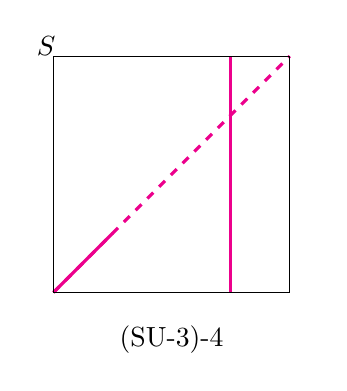
\begin{tikzpicture}[xscale=3, yscale=3]
			\node[above left] at (0.05,0.96) {$S$};
			\node[above right,text=white] at (0.95,0.95) {$C$};
			\draw [line width=0.4mm, dashed, magenta] (0,0) -- (1,1);
			\draw [line width=0.4mm, magenta] (0,0) -- (0.25,0.25);
			\draw [line width=0.4mm, magenta] (0.75,0) -- (0.75,1);
			\node[below] at (0.5,-0.1) {(SU-3)-4};
			\draw (0,0) rectangle (1,1);
		\end{tikzpicture}
	}
	\end{subfigure}\hspace{0.5cm}
	\begin{subfigure}{.2\textwidth}
		\centering
		\resizebox{\textwidth}{!}{%
		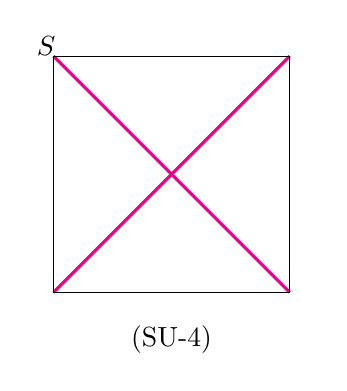
\begin{tikzpicture}[xscale=3, yscale=3]
			\node[above left] at (0.05,0.96) {$S$};
			\node[above right,text=white] at (0.95,0.95) {$C$};
			\draw [line width=0.4mm, magenta] (0,0) -- (1,1);
			\draw [line width=0.4mm, magenta] (0,1) -- (1,0);
			\node[below] at (0.5,-0.1) {(SU-4)};
			\draw (0,0) rectangle (1,1);
		\end{tikzpicture}
	}
	\end{subfigure}\hspace{0.5cm}
	\begin{subfigure}{.2\textwidth}
		\centering
		\resizebox{\textwidth}{!}{%
		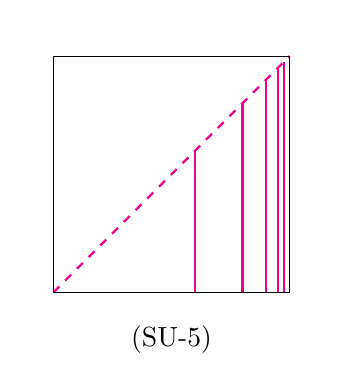
\begin{tikzpicture}[xscale=3, yscale=3]
			\node[above right,text=white] at (0.95,0.95) {$C$};
			\node[above left,text=white] at (0.05,0.96) {$S$};
			\draw [line width=0.3mm, dashed, magenta] (0,0) -- (1,1);
			\draw [line width=0.3mm, magenta] (0.6,0) -- (0.6,0.6);
			\draw [line width=0.3mm, magenta] (0.8,0) -- (0.8,0.8);
			\draw [line width=0.3mm, magenta] (0.9,0) -- (0.9,0.9);
			\draw [line width=0.3mm, magenta] (0.95,0) -- (0.95,0.95);
			\draw [line width=0.3mm, magenta] (0.975,0) -- (0.975,0.975);
			\node[below] at (0.5,-0.1) {(SU-5)};
			\draw (0,0) rectangle (1,1);
		\end{tikzpicture}
		}
	\end{subfigure}
%	\begin{subfigure}{.2\textwidth}
%		\centering
%		\begin{tikzpicture}[xscale=2, yscale=2]
%			\draw (0,0) rectangle (1,1);
%			\draw[fill=forestgreen!70] (0,0) rectangle (0.85,0.85);
%		\end{tikzpicture}
%		\caption*{(NSU-3)}
%	\end{subfigure}\vspace{0.5cm}
	\caption{Subregions of $[0,1]^2$ that are either a set of uniqueness (magenta) or not a set of uniqueness (green). The regions for which the corresponding result is only valid for strict t-norms have been marked with an ``$S$'' in the upper left corner. The regions for which the corresponding continuous completions are known have been marked with a ``$C$'' in the upper right corner.}
	\label{fig:SurveyCompletions}
\end{figure}

Finally, let us end this section with a brief discussion that relates the existing information in the literature about the topic up to our knowledge and our problem. Let $\TA : A \to [0,1]$ be a continuous and conditionally cancellative pre-t-norm where $A \subseteq [0,1]^2$ is one of the regions in Figure \ref{fig:regions}. First, it is clear that any t-norm is a completion of $T_A$ if $A$ corresponds to Region 4, because the values in the boundary are fixed for all t-norms. Besides, if $A$ is Region 8 then all the information we know about the t-norm is a horizontal/vertical section and the boundaries, so our problem is already solved and corresponds to result (C-2). On the other hand, the study of the continuous completions of pre-t-norms defined on Regions 1, 2, 3, 5, 6 and 7 is not available in the literature. So, in order to provide  the desired characterization of $(S,N)$-implications when $N$ has one point of discontinuity we have to personally study the continuous completions of pre-t-norms defined on this type of regions. Nonetheless, let us present two straightforward results: if a pre-t-norm \TB defined on $B \subseteq [0,1]^2$ can be continuously completed to a t-norm $T$, then $T$ is also a continuous completion of any restriction of \TB to a subset of $B$; and if a pre-t-norm \TB defined on $B \subseteq [0,1]^2$ can be completed and a restriction of \TB to a subset $A$ has a unique continuous completion $T$, then $T$ is also the unique completion of \TB.  


\begin{proposition}\label{prop:EquivalenceCompletionsTATB}
	Let $T_A: A \to [0,1]$, $T_B: B \to [0,1]$ be two continuous pre-t-norms defined on $A \subsetneq B \subsetneq [0,1]^2$ such that $\TA(x,y)=\TB(x,y)$ for all $(x,y) \in A$.
	\begin{enumerate}[label=(\roman*)]
		\item If $T$ is a continuous completion of $\TB$ then $T$ is also a continuous completion of $\TA$.
		\item If \TA has a unique continuous completion $T$ and \TB can be completed, then $T$ is the unique continuous completion of \TB.
	\end{enumerate} 
\end{proposition}

\begin{proof}~~
	\begin{enumerate}[label=(\roman*)]
		\item Let $T$ be a continuous completion of $\TB$, then $T(x,y)=\TB(x,y)=\TA(x,y)$ for all $(x,y) \in A$ and $T$ is also a continuous completion of $\TA$.
		\item Let $T$ be the unique continuous completion of $\TA$ and $\tilde{T}$ any continuous completion of \TB. Then, $T(x,y)=\TA(x,y)=T_B(x,y)=\tilde{T}(x,y)$ for all $(x,y) \in A$. Then $\tilde{T}$ is also a continuous completion of $\TA$ and since $T$ is the unique continuous completion of $\TA$ we obtain that $T(x,y)=\tilde{T}(x,y)$ for all $(x,y) \in [0,1]^2$. \qedhere
	\end{enumerate}
\end{proof}

Proposition \ref{prop:EquivalenceCompletionsTATB} is interesting because it gives the idea that if the study of the continuous completions of a pre-t-norm defined on a certain region $A$ is available, this result may be useful when studying bigger regions that contain $A$. For instance, all the regions in Figure \ref{fig:regions} contain at least one horizontal/vertical section and Regions 1, 2, 3, 5, 6 and 7 contain a square $[\alpha,\beta]^2 \subsetneq [0,1]^2$ , so a possible approach for our problem could be using the results (C-2) or (C-4) as starting point for solving the problem of the continuous completions of conditionally cancellative/cancellative pre-t-norms defined on these regions. On the other hand, Regions 1, 3, 5 and 7 contain a triangle with edges $(1-\varepsilon,0)$, $(1,0)$ and $(1,1)$, for some $\varepsilon \in (0,1]$, so result (SU-1) tell us that in this case if a conditionally cancellative/cancellative pre-t-norm defined on one of these regions can be continuously completed, the completion must be unique. Finally, result (SU-3) (see (SU-3)-4 in Figure \ref{fig:SurveyCompletions}) highlights that if a strict t-norm only known in a region of the type 6 can be completed, the completion must be unique. However, in this case the same result for the nilpotent case is not available and we later point out that in this case a completion might not be unique.

\subsection{Simplification to the minimum and continuous Archimedean case}

Let us now focus on the problem of finding the continuous completions of a continuous pre-t-norm $T_A$ defined on one of the regions in Figure \ref{fig:regions}. If we assume that $T_A$ can be completed to a continuous t-norm $T$, we know by the characterization of continuous t-norms that $T$ is an ordinal sum of continuous Archimedean t-norms. Thus, if a t-norm $T$ has an idempotent point $q \in (0,1)$ with $T(q,q)=q$ then there exist two continuous t-norms $T_1$ and $T_2$ such that $T=(\left\langle 0,q,T_1 \right\rangle, \left\langle q,1,T_2 \right\rangle)$. It is straightforward to prove that $T_1|_{A_1}$ and $T_2|_{A_2}$ where $\displaystyle A_1= \left\lbrace \left(\frac{x}{q},\frac{y}{q}\right) \mid (x,y) \in A \cap [0,q]^2\right\rbrace$ and $A_2 = \left\lbrace \left(\frac{x-q}{1-q},\frac{y-q}{1-q}\right) \mid (x,y) \in A \cap [q,1]^2\right\rbrace$ are two continuous pre-t-norms. Further, $A_1$ (resp. $A_2$)  corresponds to either $[0,q]^2$ (resp. $[q,1]^2$) or to an scaled version of one of the regions of Figure \ref{fig:regions}. Therefore, once we have solved the problem for continuous Archimedean t-norms and for the minimum t-norm we can use this argument to find a completion in the continuous case. 

Having said this, we have simplified the problem stated in Section \ref{subsection:decription_regions_interest} to the study of the continuous completions of a continuous pre-t-norm $T_A$ defined on one of the regions of Figure \ref{fig:regions} in two cases: when $T_A$ corresponds to the minimum and when $T_A$ is a conditionally cancellative (that may be cancellative or not) pre-t-norm.

Inspired by the literature, for the study of the second case we are interested in determining the corresponding continuous completions in terms of an additive generator.  To assume the existence of an additive generator we need to prove that the continuous completions of the pre-t-norms of interest are always continuous Archimedean t-norms. Indeed, the following result remarks the following fact: if a conditionally cancellative pre-t-norm $\TA$ is defined on a region $A$ which contains the boundaries of $[0,1]^2$ and a horizontal/vertical section, then any continuous completion of $\TA$ is necessarily a continuous Archimedean t-norm.

\begin{proposition}\label{prop:CC->ArchiCompletion}
	Let $\TA : A \to [0,1]$ be a pre-t-norm defined on $A \subseteq [0,1]^2$ such that $([0,1]^2 \setminus (0,1)^2)\cup([0,1]\times\{c\}) \cup (\{c\} \times [0,1]) \subseteq A$ with $c \in (0,1)$ which is conditionally cancellative. If $\TA$ can be completed to a continuous t-norm $T$, then $T$ is a continuous Archimedean t-norm. Moreover, if $\TA$ is cancellative then $T$ is a strict t-norm and if $\TA$ is not cancellative then $T$ is a nilpotent t-norm.
\end{proposition}
\begin{proof}
	Let $\TA : A \to [0,1]$ be a pre-t-norm defined on $A \subseteq [0,1]^2$ such that $([0,1]^2 \setminus (0,1)^2)\cup([0,1]\times\{c\}) \cup (\{c\} \times [0,1]) \subseteq A$ with $c \in (0,1)$ which is conditionally cancellative. Let $T$ be a continuous completion of \TA that is not Archimedean, then there exists an $\alpha \in (0,1)$ such that $T(\alpha,\alpha)=\alpha$. In this case, by the characterization of continuous t-norms we know that $T(x,y)=\min \{x,y\}$ for all $(x,y) \in ([0,\alpha] \times [\alpha,1]) \cup ([\alpha,1] \times [0,\alpha])$. Now, we distinguish between two cases:
	\begin{itemize}
		\item If $c \in (0,\alpha]$ then
		$$\TA(c,y)=\min \{c,y\}=c, \quad \text{for all } y \in [\alpha,1],$$
		and we obtain a contradiction with the fact that $\TA$ is a conditionally cancellative pre-t-norm.
		\item If $c \in (\alpha,1)$ then
		$$\TA(c,y)=\min \{c,y\}=y, \quad \text{for all } y \in [0,\alpha],$$
		and in this case $\TA(c,y)=y=\TA(y,1)$ for all $y \in [0,\alpha]$ which is a contradiction with the fact that $\TA$ is a conditionally cancellative pre-t-norm.
	\end{itemize}
	Now, let us assume that $\TA$ is cancellative and $T$ is nilpotent, then the induced negation of $T$ is a continuous, strictly decreasing function such that $N_T(0)=1$, $N_T(1)=0$ and $T(x,y)=0$ if and only if $y \in [0,N_T(x)]$ for all $x \in [0,1]$. Then, $0=T(c,y)=\TA(c,y)$ for all $y \in (0,N_T(c)]$ and we have a contradiction with the fact that \TA is cancellative. On the other hand, let us assume that $\TA$ is conditionally cancellative but not cancellative and $T$ is strict. We have a contradiction with the fact that there exists $(x',y') \in A$ with $x',y'>0$ such that $\TA(x',y')=T(x',y')=0$ and $T$ must be nilpotent.
\end{proof}

\subsection{Regions 4 and 8: Cases that are already solved in the literature}

To begin with, in view of the results of Section \ref{subsec:related_bibliography}, let us note that there are two cases that are already solved:
\begin{itemize}	
	\item Any t-norm is a completion of $T_A$ if $A$ corresponds to Region 4 in Figure \ref{fig:regions}, because the values on the boundary are fixed for all t-norms.
	\item If $T_A$ is a conditionally cancellative pre-t-norm and it is defined on Region 8, all the information we know about the t-norm is a horizontal section (and the corresponding vertical section by the commutativity) and the boundaries. This problem is equivalent to result (C-2) in Section \ref{subsec:related_bibliography} from which, adapting the notation to ours, we obtain the following theorem.
	\pagebreak
	\begin{theorem}\label{thm:completion-horizontalsection}
		Let $c\in(0,1)$ and $A=([0,1]^2 \setminus (0,1)^2)\cup([0,1]\times\{c\}) \cup (\{c\} \times [0,1])$. Let $T_A:A\to[0,1]$ be a continuous pre-t-norm. Then,
		\begin{enumerate}[label=(\roman*)]
			\item  If $\TA$ is cancellative, let us define $h_c : [0,1] \to [0,c]$ by $h_c(x)=T_A(c,x)=T_A(x,c)$ for all $x \in [0,1]$. Then $h_c$ is a strictly increasing function with $h_c(0)=0$ and $h_c(1)=c$. In this case $\TA$ has infinitely many continuous completions and each continuous completion $T$ corresponds to a strict t-norm with additive generator
			\begin{equation}\label{eq:can:completion-horizontalsection}
				t(x)=
				\left\{ \begin{array}{ll}
					+\infty	 &   \text{if }   x=0, \\
					n+\overline{t}(h_c^{-n}(x)) & \text{if }  x \in [c_{T_A}^{(n+1)},c_{T_A}^{(n)}), \text{ for all } n \in \NN, \\
					\overline{t}(x) & \text{if } x \in [c,1],
				\end{array} \right.
			\end{equation}
			where $c_{T_A}^{(n)}=\TA(\overbrace{c,\dots,c}^{n})$, $h_c^{-n}(x) =\overbrace{h_c^{-1}\circ \dots \circ h_c^{-1}}^n(x)$, and $\overline{t}:[c,1] \to [0,1]$ is a continuous, strictly decreasing function with $\overline{t}(c)=1$ and $t(1)=0$.
			\item If $\TA$ is conditionally cancellative but not cancellative, let us define $\NTA(c)=\max\{t \in [0,1] \mid \TA(c,t)=0\}$, $c_{T_A}^{(n)}=\TA(\overbrace{c,\dots,c}^{n})$ for all $n \in \NN$ and $h_c : [\NTA(c),1] \to [0,c]$ by $h_c(x)=T_A(c,x)=T_A(x,c)$ for all $x \in [0,1]$. Then $h_c$ is a strictly increasing function with $h_c(\NTA(c))=0$ and $h_c(1)=c$ and  there exists an $n_c \in \NN$ such that $c_{T_A}^{(n_c)}=0$ and $c_{T_A}^{(n)}>0$ for all $n < n_c$. In this case $\TA$ has infinitely many continuous completions and each continuous completion $T$ corresponds to a nilpotent t-norm with additive generator
			\begin{equation}\label{eq:concan:completion-horizontalsection}
				t(x)=
				\left\{ \begin{array}{ll}
					n+\overline{t}(h_c^{-n}(x)) & \text{if } x \in [c_{T_A}^{(n+1)},c_{T_A}^{(n)}), \text{ for all } 1 \leq n \leq n_c-1, \\
					\overline{t}(x) & \text{if } x \in [c,1],
				\end{array} \right.
			\end{equation}
			where $h_c^{-n}(x) =\overbrace{h_c^{-1}\circ \dots \circ h_c^{-1}}^n(x)$, and $\overline{t}:[c,1] \to [0,1]$ is a continuous, strictly decreasing function with $\overline{t}(c)=1$ and $t(1)=0$.
		\end{enumerate}
	\end{theorem}
\end{itemize}

\subsection{The minimum case}
Let $T_A:A \to [0,1]$ be such that $T_A(x,y)=\min\{x,y\}$ for all $(x,y) \in A$ where $A$ is one of the regions in Figure \ref{fig:regions}. Then, by considering the characterization of continuous t-norms we can directly find all the possible continuous completions of $\TA$ in this case.
\begin{proposition}\label{prop:completion-minimumcase} Let $T_A(x,y)=\min\{x,y\}$ for all $(x,y) \in A$, where $A$ is one of the regions described in Figure \ref{fig:regions}. Then, $T_A$ has infinitely many continuous completions $T:[0,1]^2 \to [0,1]$ given by the following expressions depending on the region:
	\begin{enumerate}[label=(\roman*)]
		\item If $A=[0,1]^2 \setminus (a,b)^2$ with $a,b \in [0,1]$ such that $a<b$ then
		$$
		T(x,y) =
		\left\{ \begin{array}{ll}
			a+(b-a)\cdot \tilde{T}\left(\frac{x-a}{b-a},\frac{y-a}{b-a}\right) &   \text{if }   (x,y) \in [a,b]^2, \\[.25cm]
			\min\{x,y\} & \text{otherwise,}
		\end{array} \right.
		$$
		where $\tilde{T}$ is a continuous t-norm.
		\item If $A=([0,1]^2 \setminus (a,b)^2) \cup ([0,1]\times \{c\}) \cup (\{c\}\times [0,1])$ with $a,b \in [0,1]$ and $c \in (0,1)$ such that $a<c<b$ then
		$$
		T(x,y) =
		\left\{ \begin{array}{ll}
			a+(c-a)\cdot T_1\left(\frac{x-a}{c-a},\frac{y-a}{c-a}\right) &   \text{if }   (x,y) \in [a,c]^2, \\[.25cm]
			c+(b-c)\cdot T_2\left(\frac{x-c}{b-c},\frac{y-c}{b-c}\right) &   \text{if }   (x,y) \in [c,b]^2, \\[.25cm]
			\min\{x,y\} & \text{otherwise,}
		\end{array} \right.
		$$
		where $T_1$, $T_2$ are two continuous t-norms.
	\end{enumerate}
\end{proposition}
\begin{proof} Let $T_A:A \to [0,1]$ be such that $T_A(x,y)=\min\{x,y\}$ for all $(x,y) \in A$, where $A$ is one of the regions in Figure \ref{fig:regions}. According to the characterization of continuous t-norms it is straightforward to prove that we can complete $T_A$ to a continuous t-norm $T$ by determining $T_A$ on $[0,1]^2 \setminus A$ adequately with arbitrary continuous t-norms. Having said this, we have to distinguish between two cases:
	\begin{itemize}
		\item  If $A=[0,1]^2 \setminus (a,b)^2$ with $a,b \in [0,1]$ such that $a<b$ then, we can complete $T_A$ to a continuous t-norm $T$ by considering any continuous t-norm in $[0,1]^2 \setminus A$.
		\item If $A=([0,1]^2 \setminus (a,b)^2) \cup ([0,1]\times \{c\}) \cup (\{c\}\times [0,1])$ with $a,b \in [0,1]$ and $c \in (0,1)$ such that $a<c<b$, then $c$ is an idempotent point of any possible continuous completion of $T_A$. Thus, we have to consider two continuous t-norms $T_1$ and $T_2$ in $[a,c]^2$ and $[c,b]^2$, respectively.
	\end{itemize}
\end{proof}

\begin{remark}
	Notice that Proposition \ref{prop:completion-minimumcase} solves the completion problem when the pre-t-norm is the minimum and the corresponding region is one of the regions in  Figure \ref{fig:regions}. Indeed, Case (i) encompasses Regions 1, 2, 3 and 4 and Case (ii) encompasses Regions 5, 6, 7 and 8.
\end{remark}

\subsection{Generator of a cancellative pre-t-norm defined above a level curve}

Before studying the continuous completions of cancellative or conditionally cancellative pre-t-norms defined on the regions displayed in Figure \ref{fig:regions} except for Regions 4 and 8, we study the problem of the existence and uniqueness of an additive generator of a cancellative pre-t-norm defined above a level curve. The main reason for this preliminary step is to develop an apparatus that will allow us to describe almost all the remaining completions discussed in this section in terms of an additive generator. Moreover, it was observed that knowing a piece of the generator which corresponds to a pre-t-norm defined above a level curve can be used as a starting point for almost all the cases of interest.

Specifically, the aim of this section is to show that if we know a cancellative pre-t-norm above a level curve then we can describe uniquely this part of the pre-t-norm in terms of a continuous, strictly decreasing function which behaves in the same way as an additive generator of a strict t-norm, but in the restricted area.

\begin{theorem}\label{thm:generatorabovelevelcurve}
	Let $a \in (0,1)$ and $l:[a,1] \to [a,1]$ be a continuous, strictly decreasing function such that $l^{-1}=l$, $l(a)=1$, $l(1)=a$. Let $\TA: A \to [0,1]$ be a continuous, cancellative pre-t-norm defined on $A=\{(x,y) \in [a,1]^2 \mid y \geq l(x)\}$ such that $\TA(x,l(x))=a $ for all $x \in [a,1]$. There exists a unique continuous, strictly decreasing function $t_a:[a,1] \to [0,1]$ with $t_a(a)=1$, $t_a(1)=0$,
	$$\TA(x,y)=t_a^{-1} (t_a(x)+t_a(y)), \quad x,y \in A.$$
	In this case, we say that $t_a$ is the \emph{additive generator} of $T_A$ with $t_a(a)=1$.
\end{theorem}

\begin{proof}
	The proof of this result follows a similar reasoning as the construction of generators of Archimedean t-norms \cite{Aczel1948,Alsina2006,Klement2000} or cancellative t-subnorms \cite{Mesiarova2002}. Since the corresponding proof is rather long (it encompasses Pages \pageref{subdef:powersofpretnorm}-\pageref{ex:TP:construction-abovelevelcurve}), we break its pieces into explicit definitions and lemmas. Thus, all the definitions and lemmas of this section are considered to be under the conditions of Theorem \ref{thm:generatorabovelevelcurve}. To stress this fact, the numeration of all definitions and lemmas inside this proof have the form ``\ref{thm:generatorabovelevelcurve}.X'' with $X \in \NN$.
	
	First, let us define the powers of the pre-t-norm $T_A$.
	\begin{subdefinition}\label{subdef:powersofpretnorm} Let $n \in \mathbb{N}_0$ and $x \in [a,1]$. We define the \emph{$n$-th power} of $x$ recursively
		$$x_{\TA}^{(0)}=1, \quad  x_{\TA}^{(n)}=\TA(x,x_{\TA}^{(n-1)}) \text{ when } (x,x_{\TA}^{(n-1)}) \in A.$$                                                                                   	
	\end{subdefinition}
	It is clear that the $n$-th power of a certain $x$ may not exist, for instance for $x=a$ even the second power does not exist, since $l(a)=1 >a$. More precisely, the $n$-th power of $x \in [a,1]$ exists if the $(n-1)$-th power of $x$ exists and $\displaystyle (x,x_{\TA}^{(n-1)}) \in A$. Further we define the $n$-th root of $x$. Before providing such definition, we need a preliminary result which discloses a sequence that delimits the intervals for which the $n$-th powers are well defined.
	\begin{sublemma}\label{lem:sequence}
		There exists an increasing sequence $\{b_n\}_{n \in \NN}$ such that $b_n \in (a,1)$ and
		\begin{enumerate}[label=(\roman*)]
			\item ${b_n}_{T_A}^{(n)}$ is well defined for all $n \in \NN$.
			\item $l(b_n)=\xtn{{b_n}}{n}$ for all $n \in \NN$. Thus, ${b_n}_{T_A}^{(n+1)} = a$ for all $n \in \NN$.
			\item $\xtn{x}{n+1}$ is well defined if and only if $x \in [b_n,1]$ for all $n \in \NN$.
		\end{enumerate}
	\end{sublemma}
	\begin{proof}
		We prove all the facts, including the construction of the increasing sequence $\{b_n\}_{n \in \NN}$, by induction on $n$.  Let us consider $n=1$, we know that $l$ has a fixed point $b_1 \in (a,1)$, then $l(b_1)=b_1={b_1}_{T_A}^{(1)}$. Thus, it is clear that ${b_1}_{T_A}^{(2)} = \TA(b_1,b_1)=\TA(b_1,l(b_1))=a$.  Moreover,
		$$x \geq b_1 \Rightarrow l(x) \leq l(b_1)=b_1 \leq x, \quad x < b_1 \Rightarrow l(x)>l(b_1)=b_1>x.$$
		Then,
		$$\xtn{x}{2} \text{ is well defined } \Leftrightarrow x \geq l(x) \Leftrightarrow x \geq b_1.$$
		Let us consider that for some $n \in \NN$ we have that for all $0<\tilde{n} \leq n$ there exists a $b_{\tilde{n}} \in (a,1)$ such that fulfills (i), (ii) and (iii) and let us prove the three facts for $n+1$. Let us consider the function $f(x) = l(x) - \xtn{{x}}{n+1}$ defined on $[b_n,1]$. By the induction hypothesis we know that (iii) applied to $b_n$ ensures that $f$ is well defined. On the other hand, by the continuity of $l$ and $\TA$ we deduce the continuity of $f$. Moreover,
		$$f(1)= l(1) - \xtn{{1}}{n+1} = a - 1 < 0, $$
		$$f(b_n) = l(b_n)-\xtn{{b_{n}}}{n+1} = l(b_n)-\TA(b_n, \xtn{{b_{n}}}{n}) = l(b_n) - \TA(b_n,l(b_n)) =l(b_n) -a >0.$$
		Therefore, by Bolzano's theorem there exists a $b_{n+1} \in (b_n,1)$ such that $l(b_{n+1}) =\xtn{{b_{n+1}}}{n+1}$. Moreover, ${b_{n+1}}_{T_A}^{(n+2)} = \TA(b_{n+1},{b_{n+1}}_{T_A}^{(n+1)}) = \TA(b_{n+1},l(b_{n+1}))=a$.  Finally, since $\TA$ is cancellative we have
		$$x \geq b_{n+1} \Rightarrow l(x) \leq l(b_{n+1})=\xtn{{b_{n+1}}}{n+1} \leq \xtn{x}{n+1},$$
		$$x < b_{n+1} \Rightarrow l(x)>l(b_{n+1})=\xtn{{b_{n+1}}}{n+1}>\xtn{x}{n+1},$$
		and we have
		$$\xtn{x}{n+2} \text{ is well defined } \Leftrightarrow \xtn{x}{n+1} \geq l(x) \Leftrightarrow x \geq b_{n+1}.$$	
	\end{proof}
	The next lemma is necessary for the introduction of $n$-th roots.
	\begin{sublemma}\label{lem:rationalpowers} Let $n \in \NN$, $n \geq 2$ and $x \in [a,1]$. There exists a unique $y \in [b_{n-1},1]$ such that $\xtn{y}{n}$ is well defined and $\xtn{y}{n}=x$.
	\end{sublemma}
	\begin{proof}
		Let us consider the function $f(x)= \xtn{x}{n}$ defined on $[b_{n-1},1]$, by Lemma \ref{lem:sequence} we know that this function is well defined and we know that it is continuous because \TA is. Moreover, since $T_A$ is cancellative, $f$ is strictly increasing. Then, since $f(b_{n-1})=a$ and $f(1)=1$ there exists a unique $y \in [b_{n-1},1]$ such that $\xtn{y}{n}=x$.
	\end{proof}
	In accordance with the last result, we can provide the definition of the $n$-th root of $x$ which, in contrast with the $n$-th power of $x$, exists for all $n \in \NN$, $n \geq 2$.
	\begin{subdefinition}\label{subdef:rationalpowersofpretnorm}
		Let $n \in \NN$, $n \geq 2$, and $x \in [a,1]$. The \emph{$n$-th root} of $x$, $y=\xtnf{x}{n}$, is defined recursively as the value $y \in [\xtnf{x}{n-1},1]$ such that $\xtn{y}{n}=x$.
	\end{subdefinition}
	
	The following lemma proves various properties of the $n$-th powers and the $n$-th roots.
	
	\begin{sublemma} \label{lem:1-propertiespowers}
		The following properties hold:
		\begin{enumerate}[label=(\roman*)]
			\item $\xtn{(\xtnf{x}{n})}{n}=x$ for all $x \in [a,1]$ and $n \in \NN$, $n \geq 2$.
			\item $b_i = \xtnf{a}{i+1}$ for all $i \in \NN$.
			\item $\xtnf{x}{n} \geq \xtnf{a}{n}$ for all $x \in [a,1]$ and $n \in \NN$, $n \geq 2$.
			\item The function $d_n : [\xtnf{a}{n},1] \to [a,1]$ given by $d_n(x)=\xtn{x}{n}$ is well defined, continuous and strictly increasing for all $n \in \NN$, $n \geq 2$.
			\item $\{\xtnf{x}{n}\}_{n \geq 2}$ is a strictly increasing sequence for all $x \in [a,1)$.
			\item Let $x \in [a,1]$, $k,n \in \NN$ such that $\xtn{(\xtn{x}{k})}{n}$ is well defined. Then, $\xtn{x}{kn}$ is well defined and $\xtn{(\xtn{x}{k})}{n} = \xtn{x}{kn}$.
			\item $\xtnf{(\xtnf{x}{n})}{k} = \xtnf{x}{nk}$ for all $x \in [a,1]$ and $n,k \in \NN$, $n,k \geq 2$.
		\end{enumerate}
	\end{sublemma}
	\begin{proof}
		\begin{enumerate}[label=(\roman*)]
			\item Directly from the definition.
			\item Directly from the uniqueness of the roots and Lemma \ref{lem:sequence}.
			\item Let $x \in [a,1]$ and $n \in \NN$, $n \geq 2$, then since $\TA$ is cancellative  and increasing in each variable
			$$\xtn{(\xtnf{x}{n})}{n}=x \geq a = \xtn{(\xtnf{a}{n})}{n} \Rightarrow \xtnf{x}{n} \geq \xtnf{a}{n}.$$
			\item By (iii)-Lemma \ref{lem:sequence} it is clear that $d_n$ is well defined and, since $\TA$ is continuous and cancellative, then $d_n$ is continuous and strictly increasing.
			\item Let $n \in \NN$, $n \geq 2$, by definition there exist $y \in \left[\xtnf{x}{n-1},1\right)$ and $z \in \left[\xtnf{x}{n},1\right)$ such that $\xtn{y}{n}=x$, $\xtn{z}{n+1}=x$, then
			$$\TA(1,\xtn{y}{n})=\xtn{y}{n}=x=\xtn{z}{n+1}=\TA(z,\xtn{z}{n}).$$
			Now, since $\TA$ is cancellative we have $\xtn{y}{n} < \xtn{z}{n}$ and $y<z$.
			\item Since $\xtn{(\xtn{x}{k})}{n}$ is well defined then by (iii)-Lemma \ref{lem:sequence} and Point (ii) we have that $\xtn{x}{k} \in [\xtnf{a}{n},1]$ and $x \in [\xtnf{a}{k},1]$. In this case, the powers $\xtn{(\xtn{x}{k})}{i}$ are well defined for all $i \in \{1,\dots,n\}$. Now, let us prove the claim by induction on $n$.
			\begin{itemize}
				\item If $n=1$ then  $\xtn{x}{k}$ is well defined by hypothesis and $\xtn{(\xtn{x}{k})}{1} = \xtn{x}{k}$.
				\item Let us assume that  $\xtn{x}{k\tilde{i}}$ is well defined and $\xtn{x}{k\tilde{i}} = \xtn{(\xtn{x}{k})}{\tilde{i}} \geq a$ for all $\tilde{i} \in \{1, \dots, i\}$ with $i <n$. Then,
				$$\xtn{(\xtn{x}{k})}{i+1} = \TA(\xtn{x}{k},\xtn{(\xtn{x}{k})}{i}) = \TA(\xtn{x}{k},\xtn{x}{ik}).$$
				Now, let us prove that $\xtn{x}{ik+j}$ is well defined, $\xtn{x}{ik+j} \geq a$ and $\TA(\xtn{x}{j}, \xtn{x}{ik}) = \xtn{x}{ik+j}$ for all $j \in \{1,\dots, k\}$ by induction on $j$.
				\begin{itemize}
					\item If $j=1$ then by definition $\xtn{x}{ik+1}=\TA(x, \xtn{x}{ik})$. Moreover $\TA(x, \xtn{x}{ik}) \geq\TA(\xtn{x}{k}, \xtn{x}{ik}) = \xtn{(\xtn{x}{k})}{i+1} \geq a$.
					\item Let us assume that for $\tilde{j} \in \{1,\dots j\}$ with $j<k$ we have that $\xtn{x}{ik+\tilde{j}}$ is well defined, $\xtn{x}{ik+\tilde{j}} \geq a$ and $\TA(\xtn{x}{\tilde{j}}, \xtn{x}{ik}) = \xtn{x}{ik+\tilde{j}}$. Then, by the associativity of $\TA$ we have
					\begin{eqnarray*}
					\TA(\xtn{x}{j+1}, \xtn{x}{ik}) &=& \TA(\TA(x,\xtn{x}{j}),\xtn{x}{ik}) = \TA(x,\TA(\xtn{x}{j},\xtn{x}{ik})) \\
					&=& \TA(x,\xtn{x}{ik+j}) = \xtn{x}{ik+j+1}.
					\end{eqnarray*}
					Moreover, since $j<k$, then $\xtn{x}{j+1}\geq \xtn{x}{k}$ and we have $\TA(\xtn{x}{j+1}, \xtn{x}{ik}) \geq\TA(\xtn{x}{k}, \xtn{x}{ik}) = \xtn{(\xtn{x}{k})}{i+1} \geq a$.
				\end{itemize}
				Therefore,
				$$\xtn{(\xtn{x}{k})}{i+1} = \TA(\xtn{x}{k}, \xtn{(\xtn{x}{k})}{i}) = \TA(\xtn{x}{k}, \xtn{x}{ik}) = \xtn{x}{k(i+1)}.$$
			\end{itemize}
			\item Let $y=\xtnf{(\xtnf{x}{n})}{k}$, then $y$ is such that $ y \in [\xtnf{(\xtnf{x}{n})}{k-1},1]$, $\xtn{y}{k}=\xtnf{x}{n}$, $\xtn{y}{k} \in [\xtnf{x}{n-1},1]$ and $\xtn{(\xtn{y}{k})}{n}=x$. Now, by (vi) we have $x=\xtn{(\xtn{y}{k})}{n}=\xtn{y}{kn}$ and, by unicity, $\xtnf{x}{nk}=y = \xtnf{(\xtnf{x}{n})}{k}$.
		\end{enumerate}
	\end{proof}
	By Definitions \ref{subdef:powersofpretnorm} and \ref{subdef:rationalpowersofpretnorm} we can define the rational powers for values less or equal to one for all $x \in [a,1]$.
	\begin{subdefinition}\label{subdef:rationalpowersless1}
		Let $n,m \in \NN$ such that, $n \geq 2$, $m \leq n$ and $x \in [a,1]$. We define
		$$ \xtq{x}{m}{n} = \xtn{(\xtnf{x}{n})}{m}.$$
	\end{subdefinition}
	The next lemma studies different properties of these rational powers of $T_A$.
	\begin{sublemma} \label{lem:properties_rationalpowers}
		The following properties hold:
		\begin{enumerate}[label=(\roman*)]
			\item $\xtn{(\xtnf{x}{kn})}{km} = \xtq{x}{m}{n} $ for all $x \in [a,1]$ and $n,m,k \in \NN$ with $n\geq 2$, $m \leq n$.
			\item Let $r_1,r_2 \in \QQlone$ such that $r_1 < r_2$, then $\xtn{x}{r_1} > \xtn{x}{r_2}$ for all $x \in [a,1]$.
			\item Let $r_1, r_2 \in \QQlone$ such that $r_1 + r_2 \in \QQlone$, then $\TA(\xtn{x}{r_1},\xtn{x}{r_2}) = \xtn{x}{r_1+r_2}$ for all $x \in [a,1]$.
			\item Let $r_1,r_2 \in \QQlone$, and $x \in [a,1)$ such that $\TA(\xtn{x}{r_1},\xtn{x}{r_2}) \geq x$, then $r_1 + r_2 \in \QQlone$ and $\TA(\xtn{x}{r_1},\xtn{x}{r_2}) = \xtn{x}{r_1+r_2}$.
			\item $ \displaystyle \lim_{n \to +\infty} \xtnf{x}{n} =1$ for all $x \in [a,1]$.
			\item $\{\xtq{x}{n}{n+1 }\}_{n >0}$ is a strictly decreasing sequence for all $x \in [a,1]$.
			\item $\displaystyle \lim_{n \to +\infty} \xtq{x}{n}{n+1}=x$ for all $x \in [a,1]$.
		\end{enumerate}
	\end{sublemma}
	\begin{proof}
		\begin{enumerate}[label=(\roman*)]
			\item By (i), (vi) and (vii) in Lemma \ref{lem:1-propertiespowers}
			$$\xtn{(\xtnf{x}{kn})}{km} = \xtn{(\xtn{(\xtnf{(\xtnf{x}{n})}{k})}{k})}{m} = \xtn{(\xtnf{x}{n})}{m} = \xtq{x}{m}{n}.$$
			\item Consider $p_1,q_1,p_2,q_2 \in \NN$ such that $r_1=\frac{p_1}{q_1}$ and $r_2=\frac{p_2}{q_2}$. If $q=\text{lcm}(q_1,q_2)$, there exist $m_1,m_2 \in \NN$ such that $r_1 =\frac{m_1p_1}{q}$, $r_2 = \frac{m_2p_2}{q}$ with $m_1p_1 < m_2p_2$. Now, since $\TA$ is cancellative then
			$$\xtn{x}{r_1} = \xtq{x}{m_1p_1}{q} = \xtn{(\xtnf{x}{q})}{m_1p_1} >  \xtn{(\xtnf{x}{q})}{m_2p_2} = \xtq{x}{m_2p_2}{q} = \xtn{x}{r_2}.$$
			\item Consider $p_1,q_1,p_2,q_2 \in \NN$ such that $r_1=\frac{p_1}{q_1}$ and $r_2=\frac{p_2}{q_2}$. If $q=\text{lcm}(q_1,q_2)$, there exist $m_1,m_2 \in \NN$ such that $r_1 =\frac{m_1p_1}{q}$, $r_2 = \frac{m_2p_2}{q}$ with $m_1p_1+ m_2p_2 \leq q$. Therefore, by the associativity of $\TA$ we have
			\begin{eqnarray*}
				\xtn{x}{r_1+r_2} &=& \xtn{(\xtnf{x}{q})}{m_1p_1+m_2p_2} =
				\TA\left(\xtn{(\xtn{x}{\frac{1}{q}})}{m_1p_1},\xtn{(\xtn{x}{\frac{1}{q}})}{m_2p_2}\right) = \TA\left(\xtq{x}{m_1p_1}{q},\xtq{x}{m_2p_2}{q}\right) \\
				&=& \TA(\xtn{x}{r_1},\xtn{x}{r_2}).
			\end{eqnarray*}
			\item By contrary assume that for some $x \in \left[a,1\right)$ and $r_1,r_2 \in \QQlone$ with  $\TA(\xtn{x}{r_1},\xtn{x}{r_2}) \geq x$ it holds that $1 < r_1+r_2 \leq 2$. Then, there exists an $r \in \QQlone$ with $r_1+r_2=1+r$ and, by (iii) and the associativity of $\TA$,
			$$\TA(\xtn{x}{r_1},\xtn{x}{r_2}) = \TA(\xtn{x}{r_1},\TA(\xtn{x}{1-r_1},\xtn{x}{r_2+r_1-1})) = \TA(x,\xtn{x}{r_2+r_1-1}) = \TA(x,\xtn{x}{r}) <x$$ which is a contradiction. Thus $\TA(\xtn{x}{r_1},\xtn{x}{r_2})\geq x$ implies  $r_1+r_2 \in \QQlone$ and by (iii) $\TA(\xtn{x}{r_1},\xtn{x}{r_2})=\xtn{x}{r_1+r_2}$. 	
			\item Let us consider the function $d_2 : [\xtnf{a}{2},1] \to [a,1]$ given by $d_2(x)=\xtn{x}{2}=\TA(x,x)$ which by (iv)-Lemma \ref{lem:1-propertiespowers} is a well-defined, continuous and strictly increasing function with $d_2(\xtnf{a}{2})=a$ and $d_2(1)=1$. Since $\{\xtnf{x}{n}\}_{n>0}$ is a strictly increasing function bounded by 1, its limit exists. Therefore, any convergent subsequence has to converge to the same limit. Let us consider $ \displaystyle \lim_{n \to + \infty} \xtnf{x}{2^n}=L<1$, then
			\begin{eqnarray*}
				\displaystyle \TA(L,L) &=& \TA\left(\lim_{n \to + \infty} \xtnf{x}{2^n},\lim_{n \to + \infty} \xtnf{x}{2^n}\right) = \lim_{n \to + \infty} \TA\left(\xtnf{x}{2^n},\xtnf{x}{2^n}\right) = \lim_{n \to + \infty} \xtn{(\xtnf{x}{2^n})}{2} \\
				&=& \lim_{n \to + \infty} \xtnf{x}{2^{n-1}} = L,
			\end{eqnarray*}
			and we obtain a contradiction with the fact that $\TA$ is cancellative. Then, $L=1$.
			\item Consider $n \in \NN$ and $\xtq{x}{n}{n+1} \leq \xtq{x}{n+1}{n+2}$, then since by (v)-Lemma \ref{lem:1-propertiespowers} the sequence $\{\xtnf{x}{n}\}_{n \geq 2}$ is strictly increasing and $\TA$ is cancellative we have
			$$x=\xtq{x}{n+1}{n+1} = \TA\left(\xtnf{x}{n+1},\xtq{x}{n}{n+1}\right) \leq \TA\left(\xtnf{x}{n+1},\xtq{x}{n+1}{n+2}\right) < \TA\left(\xtnf{x}{n+2},\xtq{x}{n+1}{n+2}\right) = \xtq{x}{n+2}{n+2}=x,$$
			and we obtain a contradiction.
			\item Since $\{\xtq{x}{n}{n+1}\}_{n \in \NN}$ is a strictly decreasing sequence bounded from below by $x$, its limit exists. Assume that $ \displaystyle \lim_{n \to +\infty} \xtq{x}{n}{n+1}>x$, there exists a $y \in (x,1)$ such that $ \displaystyle \lim_{n \to +\infty}  \xtq{x}{n}{n+1}>y>x$. Thus, there exists an $n_0 \in \NN$ such that $\xtq{x}{n}{n+1}>y$ for all $n \geq n_0$. Therefore,
			$$x=\xtq{x}{n+1}{n+1} = \TA\left(\xtnf{x}{n+1},\xtq{x}{n}{n+1}\right) > \TA\left(\xtnf{x}{n+1},y\right),$$
			for all $n \geq n_0$, and taking limits we obtain
			$$\lim_{n \to +\infty} x = x \geq \lim_{n \to + \infty} \TA\left(\xtnf{x}{n+1},y\right) = \TA\left(\lim_{n \to + \infty} \xtnf{x}{n+1} ,y\right) = \TA(1,y)=y,$$
			which is a contradiction.
		\end{enumerate}
	\end{proof}
	The next step is to define the inverse of the additive generator as the function that assigns to each rational number less or equal to one, the rational power of $a$. Thanks to all the previous properties, we can prove that this function is well defined, continuous and strictly decreasing. Moreover, we prove that this function can be uniquely extended to the unit interval.  To prove this last fact, we provide a preliminary general lemma which ensures that any function $f : \QQlone \to [a,1]$ with $a \in (0,1)$ which is strictly decreasing and has a dense image can be uniquely extended to a continuous, strictly decreasing function on $[0,1]$.
	\begin{sublemma}\label{lem.new}
		Assume $a\in (0,1)$ and let $f : \QQlone \to [a,1]$ be a strictly decreasing function such that $\overline{\Ran (f)} = [a,1]$.
		Then there exists a unique continuous, strictly decreasing extension of $f$,
		i.e., there exists a unique continuous, strictly decreasing function $\overline{f}: [0,1] \to [a,1]$ such that $\overline{f}(x)=f(x)$ for all $x\in \QQlone.$
	\end{sublemma}
	\begin{proof}
		First observe that for all $x\in [0,1]\setminus \mathbb{Q}$ there is $$\sup \{f(t)\mid t\in \QQlone, t>x\} = \inf \{f(t)\mid t\in \QQlone, t<x\}.$$
		Indeed, for all $s,r\in \QQlone,$ $s<x<r$ there is $f(s)>f(r)$ which implies 
		$$\inf \{f(t)\mid t\in \QQlone, t<x\}\geq f(r),$$
		and 
		$$\inf \{f(t)\mid t\in \QQlone, t<x\}\geq \sup \{f(t)\mid t\in \QQlone, t>x\}.$$
		If $\inf \{f(t)\mid t\in \QQlone, t<x\} = u > v=\sup \{f(t)\mid t\in \QQlone, t>x\}$ then $(v,u) \cap \overline{\Ran (f)} = \emptyset,$ i.e., $\overline{\Ran (f)} \neq [a,1]$,
		which is a contradiction. Thus,
		$$\sup \{f(t)\mid t\in \QQlone, t>x\} = \inf \{f(t)\mid t\in \QQlone, t<x\},$$
		and we can define a function $\overline{f}: [0,1] \to [a,1]$ by $\overline{f}(x)=f(x)$ for $x\in \QQlone$ and $\overline{f}(x)=\inf \{f(t)\mid t\in \QQlone, t<x\}$ for $x\in [0,1]\setminus \mathbb{Q}.$
		We will show that  $\overline{f}$ is continuous and strictly decreasing. Assume any $x,y\in [0,1],$ $x<y.$
		Then there exist $s,r\in \QQlone,$ $x<s<r<y.$ If $x\in \QQlone$ then $\overline{f}(x)= f(x)>f(s)=\overline{f}(s)$
		and if $x\in [0,1]\setminus \mathbb{Q}$ then 
		$$\overline{f}(x)=\inf \{f(t)\mid t\in \QQlone, t<x\}=\sup \{f(t)\mid t\in \QQlone, t>x\}\geq f(s)=\overline{f}(s),$$
		i.e., in both cases $\overline{f}(x)\geq \overline{f}(s).$ Similarly we can show $\overline{f}(r)\geq \overline{f}(y).$
		Then $\overline{f}(x)\geq \overline{f}(s)>\overline{f}(r)\geq \overline{f}(y),$ i.e., $\overline{f}(x)> \overline{f}(y)$ and thus $\overline{f}$ is strictly decreasing.
		Assume that $\overline{f}$ is not continuous. Then due to its monotonicity there exist $u,v\in [a,1],$ $u<v$ such that $(u,v) \cap \Ran (\overline{f}) = \emptyset$
		which implies $\overline{\Ran (\overline{f})} \neq [a,1]$. Therefore, since $\overline{\Ran(f)} \subseteq \overline{\Ran(\overline{f})}$ we obtain that $\overline{\Ran (f)} \neq [a,1]$, which is a contradiction.
		Finally, if $g$ is a continuous and strictly decreasing extension of $f$ then $g(x)=f(x)=\overline{f}(x)$ for all $x\in \QQlone$
		and for all $x\in [0,1]\setminus \mathbb{Q}$ there is 
		$$\sup \{f(t)\mid t\in \QQlone, t>x\} \leq g(x) \leq \inf \{f(t)\mid t\in \QQlone, t<x\},$$
		i.e., $g(x)=\overline{f}(x).$
	\end{proof}
	
	\begin{sublemma}\label{sublem:extension} The function $ t^*_a : \QQlone \to [a,1]$ given by $t^*_a(r)=\xtn{a}{r}$ is well defined, strictly decreasing with $t^*_a(0)=1$ and $t^*_a(1)=a$. Moreover, $\overline{\Ran (t^*_a)} = [a,1]$ and there exists a unique function $ \overline{t^*_a} : [0,1] \to [a,1]$  which is the continuous extension of $t^*_a$, i.e., $ \overline{t^*_a}$ is a continuous, strictly decreasing function with $\overline{t^*_a}(r)= t^*_a(r)$ for all $r \in \QQlone$.
	\end{sublemma}
	\begin{proof}
		Directly from the results of Lemma \ref{lem:properties_rationalpowers} we obtain that the function $t_a^*$ is well defined, strictly decreasing and $t_a^*(0)=1$, $t_a^*(1)=a$.
		Now, to prove the existence and uniqueness of the extension of $t_a^*$ we want to use Lemma \ref{lem.new}, so we need to prove that $\overline{\Ran (t^*_a)} = [a,1]$. Let us assume the opposite, i.e., that there exist $u,v \in (a,1)$, $u<v$, such that $ \overline{\Ran (t^*_a)} \cap (u,v)=\emptyset$. Consider
		$$u_0 = \sup \{x \in \Ran (t^*_a) \mid x \leq u\}, \quad v_0 = \inf \{x \in \Ran (t^*_a) \mid x \geq v\},$$
		we have that $u_0,v_0 \in \overline{\Ran (t^*_a)}$ and, by the definition of infimum, for all $\delta >0$ there exists a $p_{\delta} \in \QQlone$ such that $v_0 \leq \xtn{a}{p_{\delta}} \leq v_0 + \delta$. Since $\TA$ is defined on $A=\{(x,y) \in [a,1]^2 \mid y \geq l(x)\}$ and
		$$\TA(l(v_0),v_0)=a \leq u_0 , \quad \TA(v_0,1)=v_0 > u_0,$$
		there exists a $z_0 \in [l(v_0),1)$ such that $\TA(v_0,z_0)=u_0$. Now, since $\displaystyle \lim_{r \to 0^+} \xtn{a}{r}=1$ there exists an $r_0 \in \QQlone$ such that $z_0 < \xtn{a}{r_0} < 1$. Thus,
		$$ u_0 = \TA(v_0,z_0) < \TA(v_0,\xtn{a}{r_0}).$$
		Since $\TA$ is continuous, for $\varepsilon = v_0 - \TA(v_0,\xtn{a}{r_0})>0$ there exists a $\delta_{\varepsilon}>0$ such that
		$$| x- v_0 | < \delta_{\varepsilon} \Rightarrow | \TA(x,\xtn{a}{r_0}) - \TA(v_0,\xtn{a}{r_0})| < \varepsilon,$$
		then, taking $x=\xtn{a}{p_{\delta_\varepsilon}}$, since $v_0-\delta_\varepsilon < v_0 \leq \xtn{a}{p_{\delta_\varepsilon}} \leq v_0 + \delta_\varepsilon$ there is
		$$a \leq u_0 < \TA(v_0,\xtn{a}{r_0}) \leq \TA(\xtn{a}{p_{\delta_\varepsilon}},\xtn{a}{r_0}) < \varepsilon +\TA(v_0,\xtn{a}{r_0})=v_0.$$
		By (iv)-Lemma~\ref{lem:properties_rationalpowers}, $p_{\delta_\varepsilon} + r_0 \leq 1$ and $\TA(\xtn{a}{p_{\delta_\varepsilon}},\xtn{a}{r_0}) = \xtn{a}{p_{\delta_{\varepsilon}}+r_0} \in \overline{\Ran (t^*_a)} \cap (u_0,v_0)$ which is a contradiction.
		Thus $\overline{\Ran (t^*_a)} = [a,1]$ and by Lemma \ref{lem.new} there exists  a unique function $ \overline{t^*_a} : [0,1] \to [a,1]$  which is the continuous, strictly decreasing extension of $t^*_a$.
	\end{proof}
	Finally, we prove the main result. Let us define the function $t_a: [a,1] \to [0,1]$ as $t_a = \overline{t^*_a}^{-1}$, then for all $x,y \in [a,1]$ such that $t_a(x)+t_a(y) \leq 1$ by (iii)-Lemma~\ref{lem:properties_rationalpowers} we have
	\begin{eqnarray*}
		\TA(x,y) &=& \TA(t_a^{-1}(t_a(x)),t_a^{-1}(t_a(y))) = \TA(\overline{t^*_a}(t_a(x)),\overline{t^*_a}(t_a(y))) \\
		&=& \TA(\lim\limits_{\substack{r_1 \in \QQlone \\ r_1\rightarrow t_a(x)}} \at{r_1},\lim\limits_{\substack{r_2\in \QQlone \\ r_2\rightarrow t_a(y)}} \at{r_2}) = \lim\limits_{\substack{r_1,r_2 \in \QQlone \\ r_1\rightarrow t_a(x) \\ r_2\rightarrow t_a(y)}}\TA( \at{r_1}, \at{r_2})\\
		&=&\lim\limits_{\substack{r\in \QQlone \\ r\rightarrow t_a(x) +t_a(y)}}\xtn{a}{r} = \overline{t^*_a}(t_a(x)+t_a(y)) = t_a^{-1}(t_a(x)+t_a(y)).
	\end{eqnarray*}
	Note that since $\TA(x,y) \geq a$ for $(x,y) \in A$, then $\TA(x,y) =\TA(\overline{t^*_a}(t_a(x)),\overline{t^*_a}(t_a(y))) \geq a$ and by (iv)-Lemma~\ref{lem:properties_rationalpowers} $t_a(x)+t_a(y) \leq 1$.
	
	To prove the unicity, let us consider $t_a:[a,1] \to [0,1]$ and $\hat{t}_a:[a,1] \to [0,1]$ continuous, strictly decreasing functions with $t_a(a)=\hat{t}_a(a)=1$, $t_a(1)=\hat{t}_a(1)=0$ and
	$$\TA(x,y)=t_a^{-1}(t_a(x)+t_a(y)), \quad x,y \in [a,1] \text{ and } t_a(x)+t_a(y) \leq 1,$$
	$$\TA(x,y)=\hat{t}_a^{-1}(\hat{t}_a(x)+\hat{t}_a(y)), \quad x,y \in [a,1] \text{ and } \hat{t}_a(x)+\hat{t}_a(y) \leq 1.$$
	Then,
	$$t_a \circ \hat{t}_a^{-1}(\hat{t}_a(x)+\hat{t}_a(y))=t_a(x)+t_a(y), \quad x,y \in [a,1],~ t_a(x)+t_a(y) \leq 1 \text{ and } \hat{t}_a(x)+\hat{t}_a(y) \leq 1.$$
	If we consider $u = \hat{t}_a(x)$ and $v=\hat{t}_a(y)$ then
	$$t_a \circ \hat{t}_a^{-1}(u+v)=t_a\circ \hat{t}_a^{-1}(u)+t_a\circ \hat{t}_a^{-1}(v), \quad u,v \in [0,1],~ u+v \leq 1 \text{ and }t_a \circ \hat{t}_a ^{-1}(u)+t_a \circ \hat{t}_a ^{-1}(v) \leq 1.$$
	Thus, the function $f:[0,1] \to [0,1]$ given by $f= t_a \circ \hat{t}_a ^{-1}$ is continuous, strictly increasing with $f(0)=0$, $f(1)=1$ and
	\begin{equation}\label{eq:FunctionalCauchyTwoConditions}
		f(u+v)=f(u)+f(v), \quad u,v \in [0,1],~ u+v \leq 1,~ f(u)+f(v) \leq 1.
	\end{equation}
	This function corresponds to the well-known Cauchy functional equation with several restrictions. Although the solution for the restrictions $u,v \in [0,1]$, $u+v \leq 1$ is known \cite{Aczel1966}, as far as we know, there is no solution available in the literature under the assumption $f(u)+f(v) \leq 1$. Therefore, we provide explicit proof that the unique solution of Equation (\ref{eq:FunctionalCauchyTwoConditions}) is $f(x)=x$ for all $x \in [0,1]$. First, let us prove that $f\left(\frac{1}{n}\right)= \frac{1}{n}$ for all $n \in \NN$, $n \geq 2$. We distinguish between two cases:
	\begin{itemize}
		\item If $f\left(\frac{1}{n}\right) \leq \frac{1}{n}$ then $\overbrace{f\left(\frac{1}{n}\right) + \dots + f\left(\frac{1}{n}\right)}^n \leq 1$ and
		$$1=f(1)=f\left(\frac{n}{n}\right) = nf\left(\frac{1}{n}\right) \Rightarrow f\left(\frac{1}{n}\right) = \frac{1}{n}.$$
		\item If $f\left(\frac{1}{n}\right) > \frac{1}{n}$ then $f^{-1} \left(\frac{1}{n}\right)<\frac{1}{n}$ and $\overbrace{f^{-1}\left(\frac{1}{n}\right) + \dots + f^{-1}\left(\frac{1}{n}\right)}^n \leq 1$. Thus,
		$$f(1)=1 = n f \circ f^{-1} \left(\frac{1}{n}\right) = f \left(n f^{-1}\left(\frac{1}{n}\right)\right) \Rightarrow f^{-1}\left(\frac{1}{n}\right) = \frac{1}{n} \Rightarrow f \left(\frac{1}{n}\right) = \frac{1}{n}.$$
	\end{itemize}	
	\noindent Now, for $m,n \in \NN$ with, $m\leq n$ we have
	$$f \left(\frac{m}{n}\right) =m f\left(\frac{1}{n}\right) = \frac{m}{n}.$$
	Then, $f(x)=x$ for all $x \in \QQlone$ and since $f$ is continuous then $f(x)=x$ for all $x \in [0,1]$.
\end{proof}

The next two examples show the step-by-step construction of the generator described in Theorem \ref{thm:generatorabovelevelcurve} for two particular cases. Notice that these examples show that the result can be used for cancellative or conditionally cancellative pre-t-norms whenever the part above a certain level curve is available, as long as we avoid the zero region in the second case.

\begin{example}\label{ex:TP:construction-abovelevelcurve}
	Let us consider $a \in (0,1)$ and $l:[a,1] \to [a,1]$ the function defined by $l(x)=\frac{a}{x}$ for all $x \in [a,1]$. It is clear that $l$  is a strictly decreasing function with $l^{-1}=l$, $l(a)=1$ and $l(1)=a$. Let us consider $A=\{(x,y) \in [a,1]^2 \mid xy \geq a\}$ and the function $\TA: A \to [0,1]$ defined by $\TA(x,y)=xy$ for all $(x,y) \in A$. It is straightforward to see that \TA is a continuous, cancellative pre-t-norm and $\TA(x,l(x))=x\frac{a}{x}=a$ for all $x \in [a,1]$. By iteration we compute the $n$-th powers of \TA (Definition \ref{subdef:powersofpretnorm}):
	$$\xtn{x}{n}=x^n, \quad \text{for all } x \geq \sqrt[n]{a} \text{ and } n \in \NN,$$
	and the  $n$-th roots  (Definition \ref{subdef:rationalpowersofpretnorm}):
	$$\xtnf{x}{n} = \sqrt[n]{x}, \quad \text{for all } x \in [a,1] \text{ and } n \in \NN, n \geq 2.$$
	Therefore, the rational powers of $\TA$ (Definition \ref{subdef:rationalpowersless1}) are:
	$$\xtq{x}{m}{n} =  \sqrt[n]{x^m}, \quad \text{for all } x \in [a,1] \text{ and } m,n \in \NN,  n \geq 2, m \leq n.$$
	Now, the function $t_{a}^*: \QQlone \to [a,1]$ defined by $t_{a}^*(r)=a^r$ for all $r \in \QQlone$ (Lemma \ref{sublem:extension}) is a strictly decreasing function with $t_{a}^*(0)=1$ and $t_{a}^*(1)=a$. Moreover, the unique continuous extension of $t_{a}^*$ is $\overline{t_{a}^*}:[0,1] \to [a,1]$ with $\overline{t_{a}^*}(x)=a^x$ for all $x \in [0,1]$. Finally, we define $t_{a}:[a,1] \to [0,1]$ by $t_{a}(x)=\overline{t_{a}^*}^{-1}(x)=\log_a(x)$ for all $x \in [a,1]$. Then, we have
	$$t_{a}^{-1}(t_{a}(x)+t_{a}(y)) = t_{a}^{-1}\left(\log_a(x) + \log_a(y)\right) = a^{\log_a(xy)} = xy = \TA(x,y),$$
	for all $(x,y) \in [a,1]^2$ such that $t_a(x)+t_a(y)\leq 1,$ i.e.,  $\log_a(xy) \leq 1$, and then it is valid for all $(x,y) \in A$.\\
	It is clear that $\TA$ can be considered as the product t-norm above the level curve of value $a$. Therefore, the obtained generator corresponds to the generator of the product t-norm with $t(a)=1$ restricted to values $x \in  [a,1]$.
\end{example}

\begin{example}\label{ex:TLK:construction-abovelevelcurve}
	Let us consider $a \in (0,1)$ and $l:[a,1] \to [a,1]$ the function defined by $l(x)=1+a-x$ for all $x \in [a,1]$. It is clear that $l$ is a strictly decreasing function with $l^{-1}=l$, $l(a)=1$ and $l(1)=a$. Let us consider $A=\{(x,y) \in [a,1]^2 \mid x+y \geq 1+a\}$ and the function $\TA: A \to [0,1]$ defined by $\TA(x,y)=x+y-1$ for all $(x,y) \in A$. It is straightforward to see that $\TA$ is a continuous, cancellative pre-t-norm and $\TA(x,l(x))=x+1+a-x-1=a$ for all $x \in [a,1]$. By iteration we compute the $n$-th powers of $\TA$ (Definition \ref{subdef:powersofpretnorm}):
	$$\xtn{x}{n}=nx-n+1, \quad \text{for all } x \geq \frac{n-1+a}{n} \text{ and } n \in \NN,$$
	and the  $n$-th roots  (Definition \ref{subdef:rationalpowersofpretnorm}):
	$$\xtnf{x}{n} = \frac{x+n-1}{n}, \quad \text{for all } x \in [a,1] \text{ and } n \in \NN, n \geq 2.$$
	Therefore, the rational powers of $\TA$ (Definition \ref{subdef:rationalpowersless1}) are:
	$$\xtq{x}{m}{n} = m\frac{x+n-1}{n}-m+1 = 1+\frac{m}{n}(x-1), \quad \text{for all } x \in [a,1] \text{ and } m,n \in \NN,  n \geq 2, m \leq n. $$
	Now, the function $t_{a}^*: \QQlone \to [a,1]$ defined by $t_{a}^*(r)=1-(1-a)r$ for all $r \in \QQlone$ (Lemma \ref{sublem:extension}) is a strictly decreasing function with $t_{a}^*(0)=1$ and $t_{a}^*(1)=a$. Moreover, the unique continuous extension of $t_{a}^*$ is $\overline{t_{a}^*}:[0,1] \to [a,1]$ with $\overline{t_{a}^*}(x)=1-(1-a)x$ for all $x \in [0,1]$.
	Finally, we define $t_{a}:[a,1] \to [0,1]$ by $t_{a}(x)=\overline{t_{a}^*}^{-1}(x)=\frac{1-x}{1-a}$ for all $x \in [a,1]$. Then, we have
	$$t_{a}^{-1}(t_{a}(x)+t_{a}(y)) = t_{a}^{-1}\left(\frac{2-x-y}{1-a}\right) = x+y-1 = \TA(x,y),$$
	for all $(x,y) \in [a,1]^2$ such that $t_a(x)+t_a(y)\leq 1,$ i.e.,  $x+y \geq 1+a$, and then it is valid for all $(x,y) \in A$.\\
	It is clear that $\TA$ can be considered as the Łukasiewicz t-norm above the level curve of value $a$. Therefore, the obtained generator corresponds to the generator of the Łukasiewicz t-norm with $t(a)=1$ restricted to values $x \in  [a,1]$.
\end{example}

\subsection{The cancellative case}\label{subsection:cancellative_completions}

In this section we study the continuous completions of  a continuous, cancellative pre-t-norm $T_A:A \to [0,1]$ where $A$ is one of the regions in Figure \ref{fig:regions}, except Regions 4 and 8.

\subsubsection{Region 3: Continuous completions of a continuous, cancellative pre-t-norm defined on $A=[0,1]^2 \setminus (0,a)^2$ with $a \in (0,1)$}\label{subsection:can:Region3}

The aim of this section is to find the continuous completions of a continuous, cancellative pre-t-norm $T_A$ defined on $A=[0,1]^2 \setminus (0,a)^2$ with $a \in (0,1)$, solving the case of Region 3 in Figure \ref{fig:regions}.

First of all we prove that the $n$-th powers of $a$ define a partition of the interval $(0,1]$.

\begin{lemma}\label{lem:can:sequencePartitionCompletion(0,a)} Let $T_A: A \to [0,1]$ be a continuous, cancellative pre-t-norm defined on $A=[0,1]^2 \setminus (0,a)^2$ with $a \in (0,1)$. Let us define the $n$-th powers of $a$ recursively
	$$\at{0}=1, \quad \at{n}=\TA(a,\at{n-1}) \text{ for } n \in \NN.$$	
	Then $\{\at{n}\}_{n \in \mathbb{N}_0}$ is a strictly decreasing sequence and $\displaystyle \left(\bigcup_{n \in \mathbb{N}} [\at{n+1},\at{n}) \right) \cup [a,1] = (0,1]$. Thus, for every $x \in (0,1]$ there exists a unique $n \in \mathbb{N}_0$ such that $x \in  [\at{n+1},\at{n})$.
\end{lemma}

\begin{proof}
	Since \TA is cancellative and continuous, we know that $\{\at{n}\}_{n \in \mathbb{N}_0}$ is a strictly decreasing sequence whose limit exists $\displaystyle \lim_{n \to + \infty} \at{n}=L \in [0,1)$. Now, by the continuity of \TA we have
	$$\TA(1,L)=L, \quad \TA(a,L)=\TA(a,\lim_{n \to + \infty} \at{n})= \lim_{n \to + \infty} \TA(a,\at{n}) = \lim_{n \to + \infty} \at{n+1}=L.$$
	Then, since \TA is cancellative and $a \in (0,1)$ we obtain that $L=0$. Therefore, 
	$$\left(\bigcup_{n \in \mathbb{N}} [\at{n+1},\at{n}) \right) \cup [a,1] = (0,1].$$
\end{proof}

Now, we adapt the definition of horizontal/vertical section to a cancellative pre-t-norm defined on $A=[0,1]^2 \setminus (0,a)^2$ and we prove some related properties.

\begin{lemma}\label{lemma:can:Region3}
	Let $T_A: A \to [0,1]$ be a continuous, cancellative pre-t-norm defined on $A=[0,1]^2 \setminus (0,a)^2$ with $a \in (0,1)$. Let us define $h_x:[0,1] \to [0,x]$ for $x \in [a,1]$ as the function $h_x(y)=\TA(y,x)=\TA(x,y)$ for all $y \in [0,1]$. The following statements hold:
	\begin{enumerate}[label=(\roman*)]
		\item For all $x \in [a,1]$, $h_x$ is a continuous, strictly increasing function with $h_x(0)=0$ and $h_x(1)=x$.
		\item Let $n \in \NN$ and $h_a^{-n}:[0,\at{n}] \to [0,\at{n-1})$ be the function defined by $h_a^{-n} = \overbrace{h_a ^{-1} \circ \dots \circ h_a^{-1}}^n$. Then $h_a^{-n}$ is well defined, continuous and strictly increasing.
		\item Let $n,k \in \NN$ such that $k \geq n$, then $h_a^{-n}(\at{k}) = \at{k-n}$.
		\item Let $n \in \NN$, $x \in (0,\at{n}]$ and $y \in [a,1]$, then
		\begin{equation}\label{eq:can:(0,a):propha1}
		h_a^{-n}(\TA(x,y))=\TA(h_a^{-n}(x),y).
		\end{equation}
		\item Let $x,y \in [a,1)$ such that $\TA(x,y) \leq a$, then
		\begin{equation}\label{eq:can:(0,a):propha2}
		\TA(h_a^{-1}(\TA(x,y)),h_x^{-1}(a))=y.
		\end{equation}
		\item The function given by
			\begin{align*}
			h_{\bullet}^{-1}(a) \colon [a,1] &\to [a,1]\\
			x &\mapsto h_x^{-1}(a)
		\end{align*}
		is continuous and strictly decreasing.	
	\end{enumerate}
\end{lemma}

\begin{proof}
	\begin{enumerate}[label=(\roman*)]
	\item  It follows from the fact that \TA is a continuous, cancellative pre-t-norm.
	\item It follows from the definition.
	\item  It follows from Points (i) and (ii).
	\item We provide a proof by induction on $n$.
	\begin{itemize}
		\item If $n=1$ then 
		$$\TA(a,\TA(h_a^{-1}(x),y)) = \TA(\TA(a,h_a^{-1}(x)),y)=\TA(x,y),$$
		and $h_a^{-1}(\TA(x,y))=\TA(h_a^{-1}(x),y)$.
		\item We assume that Equation (\ref{eq:can:(0,a):propha1}) is true for all $\tilde{n} \leq n$ and we prove it for $n+1$. If $x \in (0,\at{n+1}]$ then
		\begin{eqnarray*}
			h_a^{n+1}(\TA(h_a^{-(n+1)}(x),y)) & = & h_a^{n}(\TA(a,\TA(h_a^{-1} \circ h_a^{-n}(x),y))) \\
			&=& h_a^{n}(\TA(\TA(a,h_a^{-1}\circ h_a^{-n}(x)),y)) \\
			&=& h_a^{n}(\TA(h_a^{-n}(x),y))=\TA(x,y),
		\end{eqnarray*}
		and $\TA(h_a^{-(n+1)}(x),y) = h_a^{-(n+1)}(\TA(x,y))$.
	\end{itemize}
	\item Applying Point (iv) with $n=1$ we obtain 
	\begin{eqnarray*}
		\TA(h_a^{-1}(\TA(x,y)),h_x^{-1}(a)) &=& h_a^{-1}(\TA(\TA(x,y),h_x^{-1}(a)))\\
		&=& h_a^{-1}(\TA(y,\TA(x,h_x^{-1}(a)))) = h_a^{-1}(\TA(y,a))=y.
	\end{eqnarray*}
	\item Let us prove that the function
	\begin{align*}
		h_{\bullet}^{-1}(a) \colon [a,1] &\to [a,1]\\
		x &\mapsto h_x^{-1}(a)
	\end{align*}
	is continuous and strictly decreasing.
	\begin{itemize}
		\item \underline{\smash{Strictly decreasing}}: Consider $a\leq y_1<y_2 \leq 1$, $x_1=h_{y_1}^{-1}(a)$ and $x_2 =h_{y_2}^{-1}(a)$. Then since $\TA$ is cancellative  $a=\TA(x_1,y_1) < \TA(x_1,y_2)$ and since $h_{y_2}$ is a strictly increasing function we obtain
		$$
		h_{y_2}(x_1)>a,~ h_{y_2}(x_2)=a \Rightarrow x_1>x_2 \Rightarrow h_{y_1}^{-1}(a) > h_{y_2}^{-1}(a).
		$$
		\item \underline{\smash{Continuous}}: Consider a decreasing sequence $\{y_n\}_{n \in \NN}$ with limit $y$, where $y,y_n \in [a,1]$ for all $n\in \NN$. We will see that the sequence $\{h_{y_n}^{-1}(a)\}_{n \in \NN}$ converges to $h_{y}^{-1}(a)$. Denote $x_n = h_{y_n}^{-1}(a)$ for all $n \in \NN$ and let $x'$ be the limit of $\{x_n\}_{n \in \NN}$, we know that this limit exists since $\{x_n\}_{n \in \NN}$ is bounded and strictly increasing. Now, since $\TA$ is continuous then $\{\TA(x_n,y_n)\}_{n \in \NN}$ converges to $\TA(x',y)$. On the other hand, $\TA(x_n,y_n)=a$ for all $n \in \NN$, then $\TA(x',y)=a$ and we get that $x' = h_{y}^{-1}(a)$. Therefore $\lim_{y_n \to y^+} h_{y_n}^{-1}(a)=h_y^{-1}(a)$. A similar argument taking an increasing sequence $\{y_n\}_{n \in \NN}$ with limit $y$, where $y,y_n \in [a,1]$ for all $n\in \NN$, shows that $\lim_{y_n \to y^-} h_{y_n}^{-1}(a)=h_y^{-1}(a)$. Thus, $h_{\bullet}^{-1}(a)$ is continuous.
	\end{itemize}
	\end{enumerate}
\end{proof}

Next, we prove that a continuous cancellative pre-t-norm $T_A$ known in $A=[0,1]^2 \setminus (0,a)^2$ with $a \in (0,1)$ can be uniquely completed to a strict t-norm. In this case, the continuous completion is given in terms of an additive generator which is defined using Theorem \ref{thm:generatorabovelevelcurve} applied to the part of $\TA$ above the level curve of value $a$.

\begin{theorem}\label{thm:can:completion(0,a)} Let $T_A: A \to [0,1]$ be a continuous, cancellative pre-t-norm defined on $A=[0,1]^2 \setminus (0,a)^2$ with $a \in (0,1)$. Let $\{\at{n}\}_{n \in \mathbb{N}_0}$ be the sequence from Lemma \ref{lem:can:sequencePartitionCompletion(0,a)}. Then $\TA$ has a unique continuous completion which is a strict t-norm $T$ with additive generator
	\begin{equation}\label{eq:can:GeneratorCompletion(0,a)}
		t(x)
		=
		\left\{ \begin{array}{ll}
			+\infty & \text{if } x=0,\\
			n+t_a(h_a^{-n}(x)) &   \text{if }   x \in [\at{n+1},\at{n}), \text{ for all } n \in \NN,\\[5pt]
			t_a(x) & \text{if } x \in [a,1],
		\end{array} \right.
	\end{equation}
	where $t_a$ is the additive generator obtained by applying Theorem \ref{thm:generatorabovelevelcurve} to the pre-t-norm $T_{A^*}: A^* \to [0,1]$ defined on $A^*=\{(x,y) \in [a,1]^2 \mid y \geq h_x^{-1}(a)\}$ by $T_{A^*}(x,y)=\TA(x,y)$ for all $(x,y) \in A^*$.
\end{theorem}

\begin{proof}
	First, we consider the function $l : [a,1] \to [a,1]$ defined by $l(x)=h_x^{-1}(a)$. By (vi)-Lemma \ref{lemma:can:Region3} we know that $l$ is a continuous, strictly decreasing function and it is straightforward to see that $l^{-1}=l$, $l(a)=1$ and $l(1)=a$. Then, the function $T_{A^*}: A^* \to [0,1]$ defined on $A^*=\{(x,y) \in [a,1]^2 \mid y \geq h_x^{-1}(a)\}$ by $T_{A^*}(x,y)=\TA(x,y)$ for all $(x,y) \in A^*$ is a continuous, cancellative pre-t-norm such that $\TA(x,l(x))=a$ for all $x \in [a,1]$. Thus, by Theorem \ref{thm:generatorabovelevelcurve} there exists a unique continuous, strictly decreasing function $t_a : [a,1] \to [0,1]$ with $t_a(a)=1$, $t_a(1)=0$ and 
	$$\TA(x,y) = T_{A^*}(x,y)=t_a^{-1}(t_a(x)+t_a(y)), \quad  \text{for all } (x,y) \in A^*.$$
	By Proposition \ref{prop:CC->ArchiCompletion} we know that any continuous completion of \TA is necessarily strict. Now, let us prove that $T$ is a continuous completion of \TA if and only if $T$ is a strict t-norm given by the additive generator $t$ in Equation (\ref{eq:can:GeneratorCompletion(0,a)}).
	\begin{description}
		\item[$(\Rightarrow)$] Let us assume that $T$ is a strict t-norm with $T(x,y)=\TA(x,y)$ for all $(x,y) \in A$.  If $x=1$ then it is clear that $t(1)=0=t_a(1)$. Let $x \in (0,1)$, by Lemma \ref{lem:can:sequencePartitionCompletion(0,a)} we know that there exists an $n \in \mathbb{N}_0$ such that $x \in [\at{n+1},\at{n})$. We prove by induction on $n$ that the additive generator of $T$ with $t(a)=1$ corresponds to Equation (\ref{eq:can:GeneratorCompletion(0,a)}) for all $x \in (0,1)$.
		\begin{itemize}
			\item If $n=0$, then $x \in [a,1)$ and by the uniqueness of the generator $t_a$ we know that $t(x)=t_a(x)$.
			\item Let us consider that the assumption is true for all $\tilde{n} \leq n$ and let us prove it for $n+1$. If $ x \in [\at{n+2},\at{n+1})$ then $a \leq h_a^{-(n+1)}(x)<1$ and we have
			$$x=\TA(a,h_a^{-1}(x)) = T(a,h_a^{-1}(x))=t^{-1}(t(a)+t(h_a^{-1}(x))).$$
			Then, since $h_a^{-1}(x) \in [\at{n+1},\at{n})$ we have
			$$t(x)=t(a)+t(h_a^{-1}(x))=1+n+t_a(h_a^{-n} \circ h_a^{-1}(x))=(n+1)+t_a(h_a^{-(n+1)}(x)).$$
		\end{itemize}
		\item[$(\Leftarrow)$] First, we prove that $t$ given by Equation (\ref{eq:can:GeneratorCompletion(0,a)}) fulfills the properties of an additive generator of a strict t-norm, i.e., we prove that $t$ is a continuous, strictly decreasing function with $t(1)=0$ and $t(0)=+\infty$.
		\begin{itemize}
			\item \underline{\smash{Continuity}}: Since $t_a$ and $h_a^{-n}$ are continuous functions we only need to evaluate the continuity in the boundary points of each interval in the definition.
			$$\lim_{x \to a^+} t(x) = t_a(a)=1,$$
			$$\lim_{x \to a^-} t(x)= 1 + t_a(h_a^{-1}(a))=1+t_a(1)=1.$$
			Let $n \in \NN$, then 
			\begin{eqnarray*}
				\lim_{x \to (\at{n})^+}t(x) &=& \lim_{x \to \at{n}} (n-1)+t_a(h_a^{-(n-1)}(x)) = (n-1)+t_a(h_a^{-n+1}(\at{n}))\\
				&=& n-1+t_a(a)=n-1+1=n,
			\end{eqnarray*}
			$$\lim_{x \to (\at{n})^-}t(x) = \lim_{x \to \at{n}} n+t_a(h_a^{-n}(x)) = n + t_a(h_a^{-n}(\at{n})) = n + t_a(1)=n.$$
			Finally,
			$$\lim_{x \to 0^+} t(x) = \lim_{n \to + \infty} \lim_{x \to (\at{n})^+} t(x) =  \lim_{n \to + \infty} n = +\infty=t(0).$$
			\item \underline{\smash{Monotonicity}}: Since $t_a$ is strictly decreasing and $h_a^{-n}$ is strictly increasing, then it is clear that $t$ is a strictly decreasing function in each interval $[\at{n+1},\at{n})$. Taking into account that $t$ is continuous in the boundary points of each interval in the definition we deduce that $t$ is a strictly decreasing function.
			\item $t(1)=t_a(1)=0$ and $t(0)=+\infty$.
		\end{itemize}
		Now, let us consider a strict t-norm $T$ with additive generator given by Equation (\ref{eq:can:GeneratorCompletion(0,a)}). To prove that $T$ is a continuous completion of \TA we need to prove that
		$$\TA(x,y)=T(x,y), \quad \text{for all } (x,y) \in A.$$
		If $x=1$ then $\TA(1,y)=y=T(1,y)$. Otherwise, since \TA is commutative, without loss of generality we consider the case $x \leq y < 1$. Then $x \in [\at{n+1},\at{n})$, $y \in [a,1)$ and $\TA(x,y) \in [\at{m+1},\at{m})$ for some $n,m \in \NN$ with $n \geq m$. Since
		$$\at{n+2}=\TA(\at{n+1},a)\leq \TA(x,y) < \TA(\at{n+1},1)=\at{n},$$
		we have two possible cases $m=n$ or $m=n+1$.
		\begin{itemize}
			\item If $m=n$ then by Equation (\ref{eq:can:(0,a):propha1}) 
			\begin{eqnarray*}
				t(\TA(x,y)) &=& n + t_a(h_a^{-n}(\TA(x,y))) = n + t_a(\TA(h_a^{-n}(x),y)) \\
				&=& n + t_a(h_a^{-n}(x)) + t_a(y) = t(x)+t(y).
			\end{eqnarray*}
			\item If $m=n+1$ then
			$$t(\TA(x,y)) = (n+1)+t_a(h_a^{-(n+1)}(\TA(x,y))) = (n+1)+t_a(h_a^{-1} \circ h_a^{-n}(\TA(x,y))),$$
			by Equation (\ref{eq:can:(0,a):propha1})  we have
			$$t(\TA(x,y))=(n+1)+t_a(h_a^{-1} \circ \TA(h_a^{-n}(x),y)),$$
			and since $h_a^{-n}(x) \geq h_a^{-n}(\at{n+1})=a$ and 
			$$\TA(h_a^{-n}(x),y)=h_a^{-n}(\TA(x,y))<h_a^{-n}(\at{n+1})=a,$$
			by Equation (\ref{eq:can:(0,a):propha2}) we obtain 
			\begin{eqnarray*}
				t(\TA(x,y)) & = &n + t_a(a) + t_a(h_a^{-1}(\TA(h_a^{-n}(x),y))) \\
				&=& n + t_a(\TA(y,h_y^{-1}(a))) + t_a(h_a^{-1}(\TA(h_a^{-n}(x),y))) \\
				&=& n + t_a(y) + t_a(h_y^{-1}(a)) + t_a(h_a^{-1}(\TA(h_a^{-n}(x),y))) \\
				&=& n + t_a(y) + t_a(\TA(h_y^{-1}(a),h_a^{-1}(\TA(h_a^{-n}(x),y)))) \\
				&=& n + t_a(y) + t_a(h_a^{-n}(x)) = t(x) + t(y).
			\end{eqnarray*}
		\end{itemize}
	\end{description}
\end{proof}

To end this section we provide an example with the step-by-step construction of the additive generator of the unique continuous completion of a continuous, cancellative pre-t-norm defined on $A=[0,1]^2 \setminus (0,a)^2$ with $a \in (0,1)$ described in Theorem \ref{thm:can:completion(0,a)} for a particular case.

\begin{example}\label{example:can:(0,a)}
	Let $a=0.8$, $A=[0,1]^2 \setminus (0,0.8)^2$ and $\TA: A \to [0,1]$ defined by $\TA(x,y)=xy$ for all $(x,y) \in A$. It is straightforward to see that $\TA$ is a continuous, cancellative pre-t-norm. The $n$-th powers of $0.8$ in this case are
	$$0.8_{\TA}^{(n)}=0.8^n, \quad \text{for all } n \in \NN.$$
	Besides, $h_{0.8}:[0,1] \to [0,0.8]$ is defined as $h_{0.8}(y)=0.8y$ for all $y \in [0,1]$ with $h_{0.8}^{-1}(x)=\frac{x}{0.8}$ for all $x \in [0,0.8]$ and then $h_{0.8}^{-n}(x)=\frac{x}{0.8^n}$ for all $x \in [ 0.8^{n+1}, 0.8^n)$ and $n \in \NN$. By the discussion in Example \ref{ex:TP:construction-abovelevelcurve} we know that $t_{0.8}(x)=\log_{0.8}(x)$ for all $x \in [0.8,1]$. Then, according to Equation (\ref{eq:can:GeneratorCompletion(0,a)}) the unique continuous completion of $\TA$ is the strict t-norm determined by the following additive generator
	$$
		t(x)
		=
		\left\{ \begin{array}{ll}
			+\infty & \text{if } x=0,\\
			n+\log_{0.8}(\frac{x}{0.8^n}) &   \text{if }   x \in [0.8^{n+1},0.8^n), \text{ for all } n \in \NN,\\[5pt]
			\log_{0.8}(x) & \text{if } x \in [0.8,1],
		\end{array} \right.
		= \log_{0.8}(x),
	$$
	for all $x \in [0,1]$. Therefore, the unique continuous completion of $\TA$ is the product t-norm.
\end{example}

\subsubsection{Region 2: Continuous completions of a continuous, cancellative pre-t-norm defined on $A=[0,1]^2 \setminus (a,1)^2$ with $a \in (0,1)$}\label{subsection:can:Region2}

The aim of this section is to find the continuous completions of a continuous, cancellative pre-t-norm $T_A$ defined on $A=[0,1]^2 \setminus (a,1)^2$ with $a \in (0,1)$, solving the case of Region 2 in Figure \ref{fig:regions}.

Differently from the previous section, for Region 2 we can directly provide the following result that ensures that a continuous, cancellative pre-t-norm $T_A$ known on the region $A=[0,1]^2 \setminus (a,1)^2$ with $a \in (0,1)$ can be uniquely completed to an Archimedean continuous t-norm, which is strict. In this case it is clear that we cannot directly use Theorem \ref{thm:generatorabovelevelcurve} because the pre-t-norm \TA is not known above any level curve. However, in this situation it is easier to prove that $\TA$ has a unique continuous completion by directly providing the expression of such completion.

\begin{theorem}\label{thm:can:completion(a,1)} Let $T_A: A \to [0,1]$ be a continuous, cancellative pre-t-norm defined on $A=[0,1]^2 \setminus (a,1)^2$ with $a \in (0,1)$. Then $\TA$ has a unique continuous completion which is the following strict t-norm $T$
	\begin{equation}\label{eq:can:Completion(a,1)}
		T(x,y)
		=
		\left\{ \begin{array}{ll}
			h_a^{-1}(\TA(x,\TA(a,y))) & \text{if } (x,y) \in (a,1)^2,\\
			\TA(x,y) &   \text{if }   (x,y) \in [0,1]^2 \setminus (a,1)^2,
		\end{array} \right.
	\end{equation}
where $h_a:[0,1] \to [0,a]$ is the function defined by $h_a(x)=\TA(x,a)=\TA(a,x)$ for all $x \in [0,1]$.
\end{theorem}

\begin{proof} Notice that since $\TA$ is a continuous, cancellative pre-t-norm the function $h_a$ is a continuous, strictly increasing function with $h_a(0)=0$ and $h_a(1)=a$. Now, let us prove that $T$ is a continuous completion of \TA if and only if $T$ is a strict t-norm given by Equation (\ref{eq:can:Completion(a,1)}).
	\begin{description}
		\item[$(\Rightarrow)$] Let $T$ be a continuous completion of $\TA$, i.e., $T(x,y)=\TA(x,y)$ for all $(x,y) \in A$. By Proposition \ref{prop:CC->ArchiCompletion} we know that $T$ is strict. Now, by the associativity of $T$ we have
		$$\TA(a,T(x,y))=T(a,T(x,y))=T(x,T(a,y))=\TA(x,\TA(a,y)),$$
		for all $(x,y) \in (a,1)^2$. Thus, $T(x,y)= h_a^{-1}(\TA(x,\TA(a,y)))$ for all $(x,y) \in A$ and $T$ must be given by Equation (\ref{eq:can:Completion(a,1)}).
		\item[$(\Leftarrow)$] First we prove that $T$ given in Equation (\ref{eq:can:Completion(a,1)}) is a strict t-norm.
		\begin{itemize}
			\item \underline{\smash{Commutativity}}: It follows directly from the commutativity and associativity of \TA and
			$$T(x,y)=h_a^{-1}(\TA(x,\TA(a,y)))=h_a^{-1}(\TA(y,\TA(a,x)))=T(y,x),$$
			for all $(x,y) \in (a,1)^2$.
			\item \underline{\smash{Neutral Element}}: It follows from the fact that $\TA$ is a pre-t-norm and $[0,1]^2 \setminus (0,1)^2 \subseteq A$.
			\item \underline{\smash{Strict monotonicity}}: If $x_1 \leq x_2$ and $\min\{x_1,x_2,y\}=0$ then it is clear that either $T(x_1,y)=0=T(x_2,y)$ or $0=T(x_1,y)<T(x_2,y)$. Let us consider $x_1,x_2,y \in (0,1]$ with $x_1 < x_2$. Let us distinguish between three cases:
			\begin{itemize}
				\item If $(x_1,y),(x_2,y) \in A$ then $T(x_1,y) = \TA(x_1,y) < \TA(x_2,y)=T(x_2,y)$.
				\item If $(x_1,y) \in A$ and $(x_2,y) \in (a,1)^2$ then $x_1 \in (0,a]$. Then, by the associativity and cancellativity of $\TA$ and monotonicity of $h_a$ we have
				\begin{eqnarray*}
				T(x_1,y) & = &\TA(x_1,y) = h_a^{-1}(\TA(a,\TA(x_1,y))) = h_a^{-1}(\TA(x_1,\TA(a,y))) \\
				 & < & h_a^{-1}(\TA(x_2,\TA(a,y))) = T(x_2,y).
				\end{eqnarray*}
				\item $(x_1,y),(x_2,y) \in (a,1)^2$ then by the cancellativity of $\TA$ and monotonicity of $h_a$ we have
				$$T(x_1,y)=h_a^{-1}(\TA(x_1,\TA(a,y))) < h_a^{-1}(\TA(x_2,\TA(a,y))) = T(x_2,y).$$
			\end{itemize}
			\item \underline{\smash{Associativity}}: If $\min \{x,y,z\}=0$, it is straightforward that $T$ fulfills the associativity, so let us assume $x,y,z \in (0,1]$. Since $T$ is commutative, we only need to prove the associativity for $x<y$. Notice that by definition we have
			$$
			\TA(a,T(x,y))
			=
			\left\{ \begin{array}{ll}
				\TA(x,\TA(a,y)) & \text{if } (x,y) \in (a,1)^2,\\
				\TA(a,\TA(x,y)) &   \text{if }   (x,y) \in [0,1]^2 \setminus (a,1)^2,
			\end{array} \right.
			=\TA(x,\TA(a,y)),
			$$
			for all $x,y \in (0,1]$. Thus,
			\begin{eqnarray*}
				\TA(a,\TA(a,T(T(x,y),z))) &=& \TA(a,\TA(T(x,y),\TA(a,z)))\\ 
										  &=& \TA(\TA(a,T(x,y)),\TA(a,z))\\
										  &=& \TA(\TA(x,\TA(a,y)),\TA(a,z)),
			\end{eqnarray*}
			\begin{eqnarray*}
				\TA(a,\TA(a,T(x,T(y,z))) &=& \TA(a,\TA(x,\TA(a,T(y,z))))\\ 
				&=& \TA(a,\TA(x,\TA(y,\TA(a,z))))\\
				&=& \TA(x,\TA(a,\TA(y,\TA(a,z))))\\
				&=& \TA(x,\TA(\TA(a,y),\TA(a,z)))\\
				&=& \TA(\TA(x,\TA(a,y)),\TA(a,z)).
			\end{eqnarray*}
			Then, by the cancellativity of $\TA$ we obtain that $\TA(a,\TA(a,T(T(x,y),z)))= \TA(a,\TA(a,T(x,T(y,z))))$ implies $T(T(x,y),z)=T(x,T(y,z))$ and $T$ is associative.
			\item \underline{\smash{Continuity}}: Since $T$ is increasing and commutative, it is enough to check that $T(x,\cdot)$ is continuous in $[0,1]$ for all $x \in [0,1]$. If $x \in [0,a]$ then $T(x,\cdot)=\TA(x,\cdot)$ is continuous because of the continuity of $\TA$. If $x=1$ then $T(1,y)=y$ for all $y \in [0,1]$ is continuous. Let us consider $x \in (a,1)$, then
			$$
			T(x,y)
			=
			\left\{ \begin{array}{ll}
				\TA(x,y) & \text{if } y \in [0,a],\\
				h_a^{-1}(\TA(x,\TA(a,y))) &   \text{if }   y \in (a,1),\\
				x & \text{if } y=1.
			\end{array} \right.
			$$
			Since $\TA$ and $h_a^{-1}$ are continuous and
			$$\lim_{y \to a^-} T(x,y)=\lim_{y \to a^-} \TA(x,y)= \TA(x,a),$$
			\begin{eqnarray*}
			\lim_{y \to a^+}T(x,y) &=& \lim_{y \to a^+} h_a^{-1}(\TA(x,\TA(a,y)))=h_a^{-1}(\TA(x,\TA(a,a)))\\
			 &=& h_a^{-1}(\TA(a,\TA(a,x)))=\TA(a,x),
			\end{eqnarray*}
			\begin{eqnarray*}
			\lim_{y \to 1^-}T(x,y) &=& \lim_{y \to 1^-}h_a^{-1}(\TA(x,\TA(a,y))) = h_a^{-1}(\TA(x,\TA(a,1)))\\
			&=& h_a^{-1}(\TA(x,a)))=x=T(x,1),
			\end{eqnarray*}
			we obtain that $T(x,\cdot)$ is continuous.
		\end{itemize}
		Finally, by the expression of $T$ in Equation (\ref{eq:can:Completion(a,1)}) it is obvious that $T$ is a continuous completion of $\TA$, i.e., $T(x,y)=\TA(x,y)$ for all $(x,y) \in [0,1]^2 \setminus (a,1)^2$.
	\end{description}
\end{proof}

The following example shows the construction of the continuous completion of a concrete continuous, cancellative pre-t-norm defined on a region of the type $[0,1]^2 \setminus (a,1)^2$ with $a \in (0,1)$ given by Theorem \ref{thm:can:completion(a,1)}.

\begin{example}\label{example:can:(a,1)}
	Let $a=0.2$, $A=[0,1]^2 \setminus (0.2,1)^2$ and $\TA: A \to [0,1]$ defined by $\TA(x,y)=xy$ for all $(x,y) \in A$. It is straightforward to see that $\TA$ is a continuous, cancellative pre-t-norm. In this case $h_{0.2} : [0,1] \to [0,0.2]$ is given by $h_{0.2}(y)=0.2y$ for all $y \in [0,1]$ and then $h_{0.2}^{-1}(x)=\frac{x}{0.2}$ for all $x \in [0,0.2]$. Thus, the unique continuous completion of \TA is given by Equation (\ref{eq:can:Completion(a,1)}), i.e., 
	$$
		T(x,y)
		=
		\left\{ \begin{array}{ll}
			\frac{0.2xy}{0.2} & \text{if } (x,y) \in (0.2,1)^2,\\
			xy &   \text{if }   (x,y) \in [0,1]^2 \setminus (0.2,1)^2,
		\end{array} \right.
		=
		xy,
	$$
	for all $x,y \in [0,1]$ and then the unique continuous completion of \TA is the product t-norm.
\end{example}

\subsubsection{Remaining regions: Regions 1, 5, 6 and 7}

The aim of this section is to find the continuous completions of a continuous, cancellative pre-t-norm $T_A$ defined on the remaining regions, i.e.,  Regions 1, 5, 6 and 7 in Figure \ref{fig:regions}.

For these cases let us point out the straightforward fact that Regions 1, 5 and 6 always contain a subregion of the type $[0,1]^2 \setminus (d,1)^2$ for some $d \in (0,1)$ and Region 7 always contains a subregion of the type $[0,1]^2 \setminus (0,e)^2$ for some $e \in (0,1)$ (see Figure \ref{fig:regions:blue}). We have already proved in Sections \ref{subsection:can:Region3} and \ref{subsection:can:Region2} that any continuous, cancellative pre-t-norm defined on these two types of regions can be completed uniquely to a strict t-norm. Therefore, by (ii)-Proposition \ref{prop:EquivalenceCompletionsTATB} it is enough to ensure that continuous, cancellative pre-t-norms defined on regions of the type 1, 5, 6 and 7 in Figure \ref{fig:regions} can be completed to the strict t-norm determined by Theorem \ref{thm:can:completion(0,a)} or \ref{thm:can:completion(a,1)}, depending on the type of subregion contained in the considered case.

\begin{figure}[t!]
	\centering
	\begin{subfigure}{.2\textwidth}
		\centering
		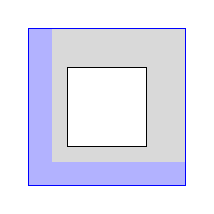
\begin{tikzpicture}[xscale=2, yscale=2]
			\draw[fill=gray!30] (0,0) rectangle (1,1);
			\fill[blue!30] (0,0) rectangle (0.15,1);
			\fill[blue!30] (0,0) rectangle (1,0.15);
			\draw[blue] (0,0) rectangle (1,1);
			\draw[fill=white!30] (0.25,0.25) rectangle (0.75,0.75);
		\end{tikzpicture}
		\caption*{Region 1:\\
			$A_1=[0,1]^2 \setminus (a,b)^2$ with $0<a<b<1$.}
	\end{subfigure}\hspace{0.5cm}
	\begin{subfigure}{.2\textwidth}
		\centering
		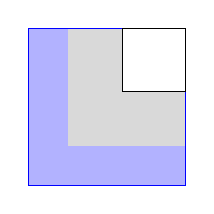
\begin{tikzpicture}[xscale=2, yscale=2]
			\draw[fill=gray!30] (0,0) rectangle (1,1);
			\fill[blue!30] (0,0) rectangle (0.25,1);
			\fill[blue!30] (0,0) rectangle (1,0.25);
			\draw[blue] (0,0) rectangle (1,1);
			\draw[fill=white!30] (0.6,0.6) rectangle (1,1);
		\end{tikzpicture}
		\caption*{Region 2:\\
			$A_2=[0,1]^2 \setminus (a,1)^2$ with $0<a<1$.}
	\end{subfigure}\hspace{0.5cm}
	\begin{subfigure}{.2\textwidth}
		\centering
		\begin{tikzpicture}[xscale=2, yscale=2]
			\draw[fill=gray!30] (0,0) rectangle (1,1);
			\fill[forestgreen!30] (0,0.75) rectangle (1,1);
			\fill[forestgreen!30] (0.75,0) rectangle (1,1);
			\draw[forestgreen] (0,0) rectangle (1,1);
			\draw[fill=white!30] (0,0) rectangle (0.4,0.4);
		\end{tikzpicture}
		\caption*{Region 3:\\
			$A_3=[0,1]^2 \setminus (0,a)^2$ with $0<a<1$.}
	\end{subfigure}\hspace{0.5cm}
	\begin{subfigure}{.2\textwidth}
		\centering
		\begin{tikzpicture}[xscale=2, yscale=2]
			\draw (0,0) rectangle (1,1);
		\end{tikzpicture}
		\caption*{Region 4:\\
			$A_4=[0,1]^2 \setminus (0,1)^2$. \\ \hspace{0.5cm} }
	\end{subfigure}\vspace{0.5cm}
	\begin{subfigure}{.2\textwidth}
		\centering
		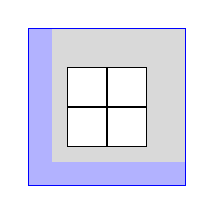
\begin{tikzpicture}[xscale=2, yscale=2]
			\draw[fill=gray!30] (0,0) rectangle (1,1);
			\fill[blue!30] (0,0) rectangle (0.15,1);
			\fill[blue!30] (0,0) rectangle (1,0.15);
			\draw[blue] (0,0) rectangle (1,1);
			\draw[fill=white!30] (0.25,0.25) rectangle (0.75,0.75);
			\draw (0.25,0.5) -- (0.75,0.5);
			\draw (0.5,0.25) -- (0.5,0.75);
		\end{tikzpicture}
		\caption*{Region 5:\\
			$A_5=([0,1]^2 \setminus (a,b)^2) \cup ([0,1] \times \{c\}) \cup (\{c\} \times [0,1])$ with $0<a<c<b<1$.}
	\end{subfigure}\hspace{0.5cm}
	\begin{subfigure}{.2\textwidth}
		\centering
		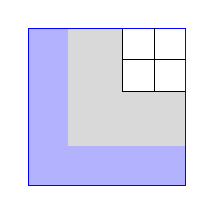
\begin{tikzpicture}[xscale=2, yscale=2]
			\draw[fill=gray!30] (0,0) rectangle (1,1);
			\draw[fill=white!30] (0.6,0.6) rectangle (1,1);
			\fill[blue!30] (0,0) rectangle (0.25,1);
			\fill[blue!30] (0,0) rectangle (1,0.25);
			\draw[blue] (0,0) rectangle (1,1);
			\draw (0.6,0.8) -- (1,0.8);
			\draw (0.8,0.6) -- (0.8,1);
		\end{tikzpicture}
		\caption*{Region 6:\\
			$A_6=([0,1]^2 \setminus (a,1)^2) \cup ([0,1] \times \{c\}) \cup (\{c\} \times [0,1])$ with $0<a<c<1$.}
	\end{subfigure}\hspace{0.5cm}
	\begin{subfigure}{.2\textwidth}
		\centering
		\begin{tikzpicture}[xscale=2, yscale=2]
			\draw[fill=gray!30] (0,0) rectangle (1,1);
			\draw[fill=white!30] (0,0) rectangle (0.4,0.4);
			\fill[forestgreen!30] (0,0.75) rectangle (1,1);
			\fill[forestgreen!30] (0.75,0) rectangle (1,1);
			\draw[forestgreen] (0,0) rectangle (1,1);
			\draw (0.4,0.2) -- (0,0.2);
			\draw (0.2,0.4) -- (0.2,0);
		\end{tikzpicture}
		\caption*{Region 7:\\
			$A_7=([0,1]^2 \setminus (0,a)^2) \cup ([0,1] \times \{c\}) \cup (\{c\} \times [0,1])$ with $0<c<a<1$.}
	\end{subfigure}\hspace{0.5cm}
	\begin{subfigure}{.2\textwidth}
		\centering
		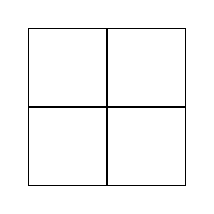
\begin{tikzpicture}[xscale=2, yscale=2]
			\draw (0,0) rectangle (1,1);
			\draw (0,0.5) -- (1,0.5);
			\draw (0.5,0) -- (0.5,1);
		\end{tikzpicture}
		\caption*{Region 8:\\
			$A_8=([0,1]^2 \setminus (0,1)^2) \cup ([0,1] \times \{c\}) \cup (\{c\} \times [0,1])$ with $0<c<1$.\\
			\hspace{0.5cm}}
	\end{subfigure}
	\caption{Regions (in gray) in which the pre-t-norms of interest for the problem of the characterization of $(S,N)$-implications are defined, if we assume that the corresponding t-conorm $S$ is continuous and the negation $N$ has only one point of discontinuity. In blue, a region of the type $[0,1]^2 \setminus (d,1)^2$ for some $d \in (0,1)$ and in green a region of the type $[0,1]^2 \setminus (0,e)^2$ for some $e \in (0,1)$.}
	\label{fig:regions:blue}
\end{figure}

Having said this, the following corollary ensures that any continuous, cancellative pre-t-norm defined on a region bigger than $A=[0,1]^2 \setminus (a,1)^2$ with some $a \in (0,1)$ is uniquely completed to the strict t-norm given by Theorem \ref{thm:can:completion(a,1)}.

\begin{corollary}\label{cor:strictcompletion1} Let $A=[0,1]^2 \setminus (a,1)^2 \subsetneq B \subsetneq [0,1]^2$ with $a \in (0,1)$ and let $T_B : B \to [0,1]$ be a continuous, cancellative pre-t-norm. Then $T_B$ has a unique continuous completion which is the strict t-norm $T$ given by Theorem \ref{thm:can:completion(a,1)} with $T_A: A \to [0,1]$ the restriction of $T_B$ to $A$.
\end{corollary}
\begin{proof}
	If we define the function $T_A :A \to [0,1]$ as the restriction of $T_B$ to $A$, then $T_A$ is a continuous, cancellative pre-t-norm. According to Theorem \ref{thm:can:completion(a,1)} we know that $T_A$ has a unique completion to a strict t-norm $T$ given by Equation (\ref{eq:can:Completion(a,1)}). Let us now prove that $T$ is also a completion of $T_B$. Consider $(x,y) \in B \setminus A$, then $x,y \in (a,1)$ and we get
	\begin{eqnarray*}
		T_A(T_B(x,y),a) &=& T_B(T_B(x,y),a) =T_B(x,T_B(y,a)) = T_A(x,T_A(y,a)) \\
		&=& T(x,T(y,a)) =T(T(x,y),a)=T_A(T(x,y),a),
	\end{eqnarray*}
	and since $T_A$ is cancellative we have $T_B(x,y)=T(x,y)$.
\end{proof}

As we have commented earlier, since Regions 1, 5 and 6 in Figure \ref{fig:regions} contain a region $A=[0,1]^2 \setminus (d,1)^2 \subsetneq B \subsetneq [0,1]^2$ with some $d \in (0,1)$ by Theorem \ref{thm:can:completion(a,1)} and Corollary \ref{cor:strictcompletion1} we obtain the unique continuous completion of continuous, cancellative pre-t-norms defined on these regions.

On the other hand, notice that Theorem \ref{thm:can:completion(0,a)} provides the unique continuous completion of a continuous, cancellative pre-t-norm defined on Region 3 in Figure \ref{fig:regions}. In accordance, the following corollary points out that Theorem \ref{thm:can:completion(0,a)} also provides the unique continuous completion of a continuous, cancellative pre-t-norm defined on Region 7 in Figure \ref{fig:regions}.

\begin{corollary}\label{cor:strictcompletion2} Let $B = ([0,1]^2 \setminus (0,a)^2) \cup ([0,1]\times \{c\}) \cup (\{c\} \times [0,1])$ with $a,c \in (0,1)$ and $c<a$ and let $T_{B}:B \to [0,1]$ be a cancellative pre-t-norm. Then, $T_B$ has a unique continuous completion which is the strict t-norm given by Theorem \ref{thm:can:completion(0,a)} with $A=[0,1]^2 \setminus (0,a)^2$ and $T_A:A \to [0,1]$ the restriction of $T_B$ to $A$.
\end{corollary}
\begin{proof}
	If we define $A=[0,1]^2 \setminus (0,a)^2$ and $T_A:A \to [0,1]$ the restriction of $T_B$ to $A$, then $T_A$ is a continuous, cancellative pre-t-norm. According to Theorem \ref{thm:can:completion(0,a)} we know that $T_A$ has a unique completion to the strict t-norm $T$ given by additive generator in Equation (\ref{eq:can:GeneratorCompletion(0,a)}). Let us prove that $T$ is also a completion of $T_B$. Due to the commutativity of \TB we only  need to prove that
	$$\TB(c,y)=T(c,y)=t^{-1}(t(c)+t(y)), \quad \text{for all } y \in (0,a).$$
	Let $y \in (0,a)$, since $c \in (0,a)$ then by Lemma \ref{lem:can:sequencePartitionCompletion(0,a)} there exist $n,m \in \NN$ such that $c \in [\at{n+1},\at{n})$ and $y \in [\at{m+1},\at{m})$. Then,
	$$t(c)=n+t_a(h_a^{-n}(c)), \quad t(y)=m+t_a(h_a^{-m}(y)).$$
	Let us prove that the following equation holds
	\begin{equation}\label{eq:(F1):strictcompletion2}
	\TB(c,y)=h_a^{n+m}(\TA(h_a^{-n}(c),h_a^{-m}(y))).
	\end{equation}
	By Equation (\ref{eq:can:(0,a):propha1}) we know that
	$$h_a^{n+m}(\TA(h_a^{-n}(c),h_a^{-m}(y)))=h_a^m(\TA(c,h_a^{-m}(y))).$$
	Now, we prove Equation (\ref{eq:(F1):strictcompletion2}) by induction on $m$:
	\begin{itemize}
		\item If $m=1$, then 
		\begin{eqnarray*}
		h_a(\TA(c,h_a^{-1}(y)))&=&\TA(a,\TA(c,h_a^{-1}(y))) = \TB(a,\TB(c,h_a^{-1}(y)))\\
		 &=& \TB(c,\TB(a,h_a^{-1}(y))) = \TB(c,\TA(a,h_a^{-1}(y))) = \TB(c,y).
		\end{eqnarray*}
		\item We assume that the fact is true for all $\tilde{m}\leq m$ and we prove it for $m+1$:
		\begin{eqnarray*}
			h_a^{m+1}(\TA(c,h_a^{-m-1}(y)))&=&h_a(h_a^m(\TA(c,h_a^{-m}(h_a^{-1}(y))))) = h_a(\TB(c,h_a^{-1}(y)))\\
			&=& \TA(a,\TB(c,h_a^{-1}(y)))=\TB(a,\TB(c,h_a^{-1}(y)))\\
			&=& \TB(c,\TB(a,h_a^{-1}(y))) = \TB(c,\TA(a,h_a^{-1}(y)))=\TB(c,y).
		\end{eqnarray*}
	\end{itemize}
	On the other hand, let $s \in \NN$ be such that $\TB(c,y) \in [\at{s+1},\at{s})$. Since \TB is associative we have
	\begin{eqnarray*}
		\TB(c,\at{m+1})&=&\TB(c,\TA(\overbrace{a,\dots,a}^{m+1})) = \TB(c,\TB(\overbrace{a,\dots,a}^{m+1}))= \overbrace{\TB(a,\TB(a,\cdots\TB(a,c)))}^{m+1} \\
		&=& \overbrace{\TA(a,\TA(a,\cdots\TA(a,c)))}^{m+1}=h_a^{m+1}(c).
	\end{eqnarray*}
	Analogously, $\TB(c,\at{m}) = h_a^{m}(c)$. Therefore,
	$$
	\TB(c,y)\geq \TB(c,\at{m+1}) =h_a^{m+1}(c) \geq h_a^{m+1}(\at{n+1})=\at{n+m+2},$$
	$$\TB(c,y) < \TB(c,\at{m}) = h_a^{m}(c) < h_a^{m}(\at{n}) = \at{n+m}.$$
	Accordingly, we have two possible cases: $s=n+m$ or $s=n+m+1$.
	\begin{itemize}
		\item If $s=m+n$ then by Equation (\ref{eq:(F1):strictcompletion2}) we have
		\begin{eqnarray*}
			t(\TB(c,y)) &=& n + m + t_a(h_a^{-n-m}(\TB(c,y)))) = n + m + t_a(\TA(h_a^{-n}(c),h_a^{-m}(y))) \\
			&=& n + m + t_a(h_a^{-n}(c)) + t_a(h_a^{-n}(y))=t(c)+t(y).
		\end{eqnarray*}
		\item If $s=m+n+1$ then by Equation (\ref{eq:(F1):strictcompletion2}) and the fact that $T$ is a completion of \TA we have
		\begin{eqnarray*}
			t(\TB(c,y)) &=& n + m + 1 + t_a(h_a^{-n-m-1}(\TB(c,y)))) \\
			&=& n + m + t_a(a) + t_a(h_a^{-n-m-1}(\TB(c,y)))) \\
			&=& n + m + t(\TA(a,h_a^{-n-m-1}(\TB(c,y))))  \\
			&=& n + m + t(h_a^{-n-m}(\TB(c,y)))\\
			&=& n + m + t(\TA(h_a^{-n}(c),h_a^{-m}(y))) \\
			&=&  n + m + t(T(h_a^{-n}(c),h_a^{-m}(y)))\\
			&=& n + m + t(h_a^{-n}(c)) + t(h_a^{-m}(y)) \\
			&=& n + m + t_a(h_a^{-n}(c)) + t_a(h_a^{-m}(y)) \\
			&=& t(c)+t(y).
		\end{eqnarray*}
	\end{itemize}
\end{proof}

\begin{remark}
	In view of Corollaries \ref{cor:strictcompletion1} and \ref{cor:strictcompletion2} it is clear that if we have a continuous, cancellative pre-t-norm defined on regions of the type 1, 5, 6 or 7 in Figure \ref{fig:regions} then in order to construct its respective unique continuous completion, we have to first identify a subregion of the type $A=[0,1]^2 \setminus (0,a)^2$ or $A=[0,1]^2 \setminus (a,1)^2$ and then proceed as in Theorems \ref{thm:can:completion(0,a)} or \ref{thm:can:completion(a,1)}, respectively. Then, the procedure of the construction of the unique continuous completion in these cases is exactly the same as the one exposed in Examples \ref{example:can:(0,a)} or \ref{example:can:(a,1)}, respectively.
\end{remark}

\subsection{The conditional cancellative case}\label{subsection:completions_conditionalcase}

In this section we study the continuous completions of  a continuous, conditionally cancellative but not cancellative pre-t-norm $T_A:A \to [0,1]$ where $A$ is one of the regions in Figure \ref{fig:regions}, except for Regions 4 and 8.

\subsubsection{Region 3: Continuous completions of a continuous, conditional cancellative pre-t-norm defined on $A=[0,1]^2 \setminus (0,a)^2$ with $a \in (0,1)$}\label{subsubsection:cc:completions(0,a)}

The aim of this section is to find the continuous completions of a continuous, conditionally cancellative but not cancellative pre-t-norm defined on $A=[0,1]^2 \setminus (0,a)^2$, solving the case for Region 3 in Figure \ref{fig:regions}.

First of all, we point out that if $\TA(a,a)=0$ the continuous completion in this case is straightforward by the properties of triangular norms.
\begin{proposition}\label{prop:CompletionCase(0,a)TA(a,a)=0}
	Let $T_A: A \to [0,1]$ be a continuous, conditionally cancellative but not cancellative pre-t-norm defined on $A=[0,1]^2 \setminus (0,a)^2$ with $a \in (0,1)$ and $\TA(a,a)=0$. Then the pre-t-norm $\TA$ has a unique continuous completion given by the following nilpotent t-norm $T$
	\begin{equation}\label{eq:trivialCompletion}
		T(x,y)
		=
		\left\{ \begin{array}{ll}
			\TA(x,y) & \text{if } (x,y) \in A, \\
			0 & \text{otherwise.}
		\end{array}\right.
	\end{equation}
\end{proposition}

\begin{proof}
	It is clear by the monotonicity in the definition of a t-norm that if there exists a continuous completion of $T_A$ it must correspond to the function in Equation (\ref{eq:trivialCompletion}). Thus, we need to prove that $T$ in Equation (\ref{eq:trivialCompletion}) is indeed a nilpotent t-norm. The continuity, neutral element, commutativity and monotonicity are trivial, so to ensure that $T$ is a continuous t-norm we only need to prove the associativity. We distinguish between different cases:
	\begin{itemize}
		\item If $(y,z), (x,T(y,z)), (x,y), (T(x,y),z) \in A$ then the associativity is ensured by the properties of pre-t-norm $\TA$.
		\item If $(y,z) \not \in A$ then $y,z \in (0,a)$ and we have $T(x,T(y,z)) = \TA(x,0) = 0$. Now, we distinguish between two more cases:
		\begin{itemize}
			\item If $T(x,y)>0$ then $(x,y) \in A$. Thus, $T(x,y)=\TA(x,y) \leq y <a$ and $(T(x,y),z) \not \in A$. Then, by definition $T(T(x,y),z)=0$.
			\item If $T(x,y)=0$ then $T(T(x,y),z)=\TA(0,z)=0$.
		\end{itemize}
		\item If $(x,y) \not \in A$ the proof is analogous to the previous case.
		\item If  $(y,z),(x,y) \in A$ and $(x,\TA(y,z)) \not \in A$ then $x,\TA(y,z) \in (0,a)$, $y \in [a,1]$ and $T(x,\TA(y,z))=0$. We distinguish between two more cases:
		\begin{itemize}
			\item If $(\TA(x,y),z) \not \in A$ then $T(\TA(x,y),z)=0$.
			\item If $(\TA(x,y),z) \in A$ then since $\TA(x,y) \leq x < a$ we have $z \in [a,1]$. Now,  since $\TA(y,0)=0$ and $\TA(y,1)=y \geq a$, by the continuity of $\TA$ there exists a $w \in (0,1]$ such that $\TA(y,w)=a$. By the conditionally cancellativity of $\TA$, $0<\TA(y,z)<a=\TA(y,w)$ implies that $z<w$. Thus,
			$$\TA(\TA(x,y),z) \leq \TA(\TA(x,y),w)=\TA(x,\TA(y,w)) = \TA(x,a) \leq \TA(a,a)=0.$$
		\end{itemize}
		\item If  $(y,z),(x,y) \in A$ and $(\TA(x,y),z) \not \in A$ the proof is analogous to the previous case.
	\end{itemize}
	Finally, the conditionally cancellativity (and non-cancellativity) of $\TA$ ensures that $T$ is a nilpotent t-norm.
\end{proof}

For the case $\TA(a,a)>0$ we start by proving that the $n$-th powers of $a$ define a finite partition of the interval $[0,1]$.

\begin{lemma}\label{lem:sequencePartitionCompletion(0,a)} Let $T_A: A \to [0,1]$ be a continuous, conditionally cancellative but not cancellative pre-t-norm defined on $A=[0,1]^2 \setminus (0,a)^2$ with $a \in (0,1)$ and $\TA(a,a)>0$. Let us define the $n$-th powers of $a$ recursively
	$$\at{0}=1, \quad \at{n}=\TA(a,\at{n-1}) \text{ for } n \in \NN.$$	
	There exists an $n_a \in \NN$ such that the finite sequence $\{\at{n}\}_{n=0}^{n=n_a}$ is a strictly decreasing sequence  with $\at{n_a}=0$ and $\left(\bigcup_{n=1}^{n_a-1} [\at{n+1},\at{n})\right) \cup [a,1] = [0,1]$.
\end{lemma}
\begin{proof}
	Since $\TA$ is conditionally cancellative, it is clear that if $\at{n_1},\at{n_2} \not = 0$ with $n_1<n_2$ then $\at{n_1}>\at{n_2}$. If there exists an $n_a \in \NN$ such that $\at{n_a}=0$ we have finished, otherwise let us assume that $\at{n}>0$ for all $n \in \NN$. If we consider $\displaystyle L=\lim_{n \to +\infty} \at{n}>0$ then $\TA(1,L)=L>0$ and
	$$L=\lim_{n \to + \infty} \at{n} = \lim_{n \to + \infty} \TA(a,\at{n-1}) = \TA(a,\lim_{n \to + \infty} \at{n-1}) = \TA(a,L),$$
	and since $\TA$ is conditionally cancellative we obtain a contradiction with the fact that $a \in (0,1)$. Thus $\displaystyle \lim_{n \to + \infty} \at{n} =0$. Now, since $\TA$ is not cancellative, there exist $(x,y) \in A$ with $x,y>0$ and $\TA(x,y)=0$. Since $\TA(a,a)>0$ then $x< a$ or $y < a$, without loss of generality we consider $x \in (0,a)$ and $y \in [a,1]$. Now, since $\displaystyle \lim_{n \to + \infty} \at{n} =0$ there exists an $n \in \NN$ such that $\at{n}<x$ and then
	$$0=\TA(x,y) \geq \TA(\at{n},a)=\TA(a,\at{n})=\at{n+1},$$
	which is a	contradiction with the fact that $\at{n}>0$ for all $n \in \NN$. Therefore,
	$$\left(\bigcup_{n=1}^{n_a-1} [\at{n+1},\at{n})\right) \cup [a,1] = [0,1].$$
\end{proof}

Now, we adapt the definitions of induced negation and horizontal section to a conditionally cancellative but not cancellative pre-t-norm defined on $[0,1]^2 \setminus (0,a)^2$ with $a \in (0,1)$. Due to the continuity of \TA, we can define the concept of induced pre-negation of \TA analogously to the definition of induced negation for nilpotent t-norms, i.e., as the maximum value that makes $\TA(x,\cdot)$ zero.

\begin{definition}
	Let $T_A: A \to [0,1]$ be a continuous, conditionally cancellative but not cancellative pre-t-norm defined on $A=[0,1]^2 \setminus (0,a)^2$ with $a \in (0,1)$ and $\TA(a,a)>0$. Then we define
	\begin{itemize}
		\item $\NTA:[a,1] \to [0,1]$ in the following way
		$$\NTA(x)=\max \{t \in [0,1] \mid \TA(x,t)=0\}.$$
		\item $h_x : [\NTA(x),1] \to [0,x]$ for $ x \in [a,1]$ as the function defined by $h_x(y)=\TA(y,x)=\TA(x,y)$ for all $y \in [\NTA(x),1]$.
	\end{itemize}
\end{definition}

The next proposition proves different properties of the induced pre-negation and the horizontal section of the pre-t-norm $\TA$. Some of the properties are straightforward, proving that these two functions play an analogous role as in the case of t-norms and other properties are a bit more unintuitive, but are of the utmost importance as they relate the known part of the pre-t-norm with the part to be determined.


\begin{lemma}\label{lem:CompletionCase(0,a)HorizontalSection}
	Let $T_A: A \to [0,1]$ be a continuous, conditionally cancellative but not cancellative pre-t-norm defined on $A=[0,1]^2 \setminus (0,a)^2$ with $a \in (0,1)$ and $\TA(a,a)>0$. Assume $n_a \in \NN$ given by Lemma \ref{lem:sequencePartitionCompletion(0,a)}. The following statements hold.
	\begin{enumerate}[label=(\roman*)]
		\item $\TA(x,y)=0$ if and only if $\NTA(x) \geq y$ for $x \in [a,1]$, $y \in [0,1]$.
		\item $T_A(x,\NTA(x))=0$ for all $x \in [a,1]$.
		\item $\NTA$ is decreasing and $\NTA(1)=0$.
		\item For all $x \in [a,1]$,  $h_x$ is a continuous, strictly increasing function with $h_x(\NTA(x))=0$ and $h_x(1)=x$.
		\item Let $n,k \in \NN$, $n,k<n_a$ such that $k \geq n$, then
		$$h_a^{-n}(\at{k}) = \at{k-n}, \quad
		\text{where } h_a^{-n} = \overbrace{h_a^{-1} \circ \dots \circ h_a^{-1}}^n$$.
		\item Let $n \in \NN$, $n < n_a$, $x \in [0,\at{n}]$ and $y \in [a,1]$ such that $x>\NTA(y)$, then $h_a^{-n}(\TA(x,y))$ and $h_a^{-n}(x)$ are well defined and
		\begin{equation}\label{eq:CompletionCase(0,a)Propertyha1}
			h_a^{-n}(\TA(x,y))=\TA(h_a^{-n}(x),y).
		\end{equation}
		\item Let $x,y \in [a,1)$ such that $\TA(x,y) \leq a$, then
		\begin{equation}\label{eq:CompletionCase(0,a)Propertyha2}
			\TA(h_a^{-1}(\TA(x,y)),h_x^{-1}(a))=y.
		\end{equation}
		\item $\TA(\at{n},h_a^{-n}(x))=x$ for all $x \in [\at{n+1},\at{n})$ and $0 \leq n \leq n_a-1$.
		\item $h_y^{-1}(z) < h_x^{-1}(z)$ for all $x,y \in [a,1]$ with $x<y$ and $z \in (0,x]$.
		\item $\NTA(y)=\TA(x,h_y^{-1}(\NTA(x)))$ for all $x,y \in [a,1]$.
		\item $\NTA$ is strictly decreasing and continuous.
	\end{enumerate}
\end{lemma}
\begin{proof}
	\begin{enumerate}[label=(\roman*)]
		\item It follows from the definition.
		\item Follows from the definition.
		\item Follows from the definition and the monotonicity of $\TA$.
		\item It follows from Point (i) and the fact that $T_A$ is continuous and conditionally cancellative.
		\item It follows from the definition.
		\item We provide a proof by induction on $n$.
		\begin{itemize}
			\item If $n=1$, then $0<\TA(x,y) \leq x \leq a$ and $h_a^{-1}(\TA(x,y))$ and $h_a^{-1}(x)$ are well defined, then
			\begin{eqnarray*}
			\TA(a,\TA(h_a^{-1}(x),y)) &=& \TA(\TA(a,h_a^{-1}(x)),y)=\TA(x,y)>0 \Rightarrow h_a^{-1}(\TA(x,y)) \\ &=&\TA(h_a^{-1}(x),y).
			\end{eqnarray*}
			\item We assume that Equation (\ref{eq:CompletionCase(0,a)Propertyha1}) is true for all $\tilde{n} \leq n$ and we prove it for $n+1$. If $x \in [0,\at{n+1}]$ and $y \in [a,1]$ then
			$$h_a^{-n}(\TA(x,y)) \leq h_a^{-n}(x) \leq h_a^{-n}(\at{n+1}) =a,$$
			and $h_a^{-(n+1)}(\TA(x,y))$ and $h_a^{-(n+1)}(x)$ are well defined. Then, we have
			\begin{eqnarray*}
				h_a^{n+1}(\TA(h_a^{-(n+1)}(x),y))&=&h_a^{n}(\TA(a,\TA(h_a^{-1} \circ h_a^{-n}(x),y))) \\
				&=& h_a^{n}(\TA(\TA(a,h_a^{-1} \circ h_a^{-n}(x)),y))\\
				&=&h_a^n(\TA(h_a^{-n}(x),y)) = \TA(x,y)>0.
			\end{eqnarray*}
			Thus,
			$$\TA(h_a^{-(n+1)}(x),y) = h_a^{-(n+1)}(\TA(x,y)).$$
		\end{itemize}
		\item Applying Point (vi) with $n=1$ we obtain
		\begin{eqnarray*}
			\TA(h_a^{-1}(\TA(x,y)),h_x^{-1}(a)) &=&h_a^{-1}(\TA(\TA(x,y),h_x^{-1}(a)))=h_a^{-1}(\TA(y,\TA(x,h_x^{-1}(a)))) \\
			&=&h_a^{-1}(\TA(y,a))=y.
		\end{eqnarray*}
		\item We prove it by induction on $n$.
		\begin{itemize}
			\item If $n=1$ then $\TA(a,h_a^{-1}(x))=x$ by definition.
			\item We consider that is true for all $\tilde{n} \leq n$  and we prove it for $n+1$.
			\begin{eqnarray*}
				\TA(\at{n+1},h_a^{-n-1}(x)) &=& \TA(\TA(a,\at{n}),h_a^{-n-1}(x)) \\
				&=& \TA(a,\TA(\at{n},h_a^{-n}(h_a^{-1}(x)))) \\
				&=& \TA(a,h_a^{-1}(x))=x.
			\end{eqnarray*}
		\end{itemize}
		\item Since $\TA$ is conditionally cancellative we have
		$$0<z=\TA(y,h_y^{-1}(z))=\TA(x,h_x^{-1}(z)) \Rightarrow h_y^{-1}(z)<h_x^{-1}(z).$$
		\item We want to prove that
		$$\TA(x,h_{y}^{-1}(\NTA(x))) = \max \{ t \in [0,1] \mid \TA(y,t)=0\},$$
		and this is equivalent to prove that $\TA(y,\TA(x,h_{y}^{-1}(\NTA(x))))=0$ and for any $w>\TA(x,h_{y}^{-1}(\NTA(x)))$ we have $\TA(y,w)>0$. Since $\TA(a,a)>0$ by Point (i)  we know that $\NTA(a)<a$, then by Point (iii) $\NTA(x) \leq \NTA(a)<a \leq y$. Having said this, we first prove that $\TA(y,\TA(x,h_y^{-1}(\NTA(x))))=0$,
		$$\TA(y,\TA(x,h_y^{-1}(\NTA(x)))) = \TA(x,\TA(y,h_y^{-1}(\NTA(x)))) = \TA(x,\NTA(x))=0.$$
		On the other hand, since $ y > \NTA(x)$ we have $h_y^{-1}(\NTA(x))<1$ and 
		$$\TA(x,h_y^{-1}(\NTA(x)))<x.$$
		 Thus,  we can consider a $w \in [0,x]$ with $w > \TA(x,h_y^{-1}(\NTA(x)))$, then
		\begin{eqnarray*}
			w > \TA(x,h_y^{-1}(\NTA(x))) &\Rightarrow &h_x^{-1}(w) > h_x^{-1}(\TA(x,h_y^{-1}(\NTA(x))))=h_y^{-1}(\NTA(x))  \\
			&\Rightarrow& \TA(y,h_x^{-1}(w)) > \NTA(x),
		\end{eqnarray*}
		and by the definition of $\NTA$ we have
		$$0<\TA(x,\TA(y,h_x^{-1}(w)))=\TA(y,\TA(x,h_x^{-1}(w)))=\TA(y,w).$$
		\item Since $\TA(a,a)>0$ we have $\NTA(a)<a$ and if in Point (x) we select $x=a$ then we obtain that $\NTA(y)=\TA(a,h_y^{-1}(\NTA(a)))$ for all $y \in [a,1]$. Let us prove that the function
		\begin{align*}
			h_{\bullet}^{-1}(\NTA(a)) \colon [a,1] &\to [\NTA(a),h_a^{-1}(\NTA(a))]\\
			y &\mapsto h_y^{-1}(\NTA(a))
		\end{align*}
		is continuous and strictly decreasing.
		\begin{itemize}
			\item \underline{\smash{Strictly decreasing}}: Consider $a\leq y_1<y_2 \leq 1$, $x_1=h_{y_1}^{-1}(\NTA(a))$ and $x_2 =h_{y_2}^{-1}(\NTA(a))$. Then since $\TA$ is conditionally cancellative  $\NTA(a)=\TA(x_1,y_1) < \TA(x_1,y_2)$ and since $h_{y_2}$ is a strictly increasing function we obtain
			$$
			h_{y_2}(x_1)>\NTA(a),~ h_{y_2}(x_2)=\NTA(a) \Rightarrow x_1>x_2 \Rightarrow h_{y_1}^{-1}(\NTA(a)) > h_{y_2}^{-1}(\NTA(a)).
			$$
			\item \underline{\smash{Continuous}}: Consider a decreasing sequence $\{y_n\}_{n \in \NN}$ with limit $y$, where $y,y_n \in [a,1]$ for all $n\in \NN$. We will see that the sequence $\{h_{y_n}^{-1}(\NTA(a))\}_{n \in \NN}$ converges to $h_{y}^{-1}(\NTA(a))$. Denote $x_n = h_{y_n}^{-1}(\NTA(a))$ for all $n \in \NN$ and let $x'$ be the limit of $\{x_n\}_{n \in \NN}$, we know that this limit exists since $\{x_n\}_{n \in \NN}$ is bounded and strictly increasing. Now, since $\TA$ is continuous then $\{\TA(x_n,y_n)\}_{n \in \NN}$ converges to $\TA(x',y)$. On the other hand, $\TA(x_n,y_n)=\NTA(a)$ for all $n \in \NN$, then $\TA(x',y)=\NTA(a)$ and we get that $x' = h_{y}^{-1}(\NTA(a))$. Therefore $\lim_{y_n \to y^+} h_{y_n}^{-1}(\NTA(a))=h_y^{-1}(\NTA(a))$. A similar argument taking an increasing sequence $\{y_n\}_{n \in \NN}$ with limit $y$, where $y,y_n \in [a,1]$ for all $n\in \NN$, shows that $\lim_{y_n \to y^-} h_{y_n}^{-1}(\NTA(a))=h_y^{-1}(\NTA(a))$. Thus, $h_{\bullet}^{-1}(\NTA(a))$ is continuous.
		\end{itemize}
		Thus, \NTA is continuous and strictly decreasing since it is the composition of the continuous functions \TA and $h_{\bullet}^{-1}(\NTA(a))$, where $T_A(a,\cdot)$ is strictly increasing on $[\NTA(a),h_a^{-1}(\NTA(a))]$ and $h_{\bullet}^{-1}(\NTA(a))$ is strictly decreasing. 
	\end{enumerate}
\end{proof}

Now, we present the main result of this section, which is the proof that a conditionally cancellative but not cancellative pre-t-norm defined on $[0,1]^2 \setminus (0,a)^2$ with $a \in (0,1)$ can be uniquely completed to a nilpotent t-norm. We prove this fact by explicitly providing the generator of the completion, which is defined using the generator constructed in Theorem \ref{thm:generatorabovelevelcurve}.

\begin{theorem}\label{thm:completion(0,a)} 
	Let $T_A: A \to [0,1]$ be a continuous, conditionally cancellative but not cancellative pre-t-norm defined on $A=[0,1]^2 \setminus (0,a)^2$ with $a \in (0,1)$ and $\TA(a,a)>0$. Let $\{\at{n}\}_{n=0}^{n=n_a}$ be the sequence from Lemma \ref{lem:sequencePartitionCompletion(0,a)}. Then $\TA$ has a unique continuous completion which is a nilpotent t-norm $T$ with additive generator
	\begin{equation}\label{eq:GeneratorCompletion(0,a)}
		t(x)
		=
		\left\{ \begin{array}{ll}
			n+t_a(h_a^{-n}(x)) &   \text{if }   x \in [\at{n+1},\at{n}), \text{ for all } 1 \leq n \leq n_a-1,\\[5pt]
			t_a(x) & \text{if } x \in [a,1],
		\end{array} \right.
	\end{equation}
	where $t_a$ is the additive generator obtained by applying Theorem \ref{thm:generatorabovelevelcurve} to the pre-t-norm $T_{A^*}: A^* \to [0,1]$ defined on $A^*=\{(x,y) \in [a,1]^2 \mid y \geq h_x^{-1}(a)\}$ by $T_{A^*}(x,y)=\TA(x,y)$ for all $(x,y) \in A^*$.
\end{theorem}
\begin{proof}
	First of all, notice that if we consider the function $l:[a,1] \to [a,1]$ defined by $l(x)=h_x^{-1}(a)$, analogously to (xi)-Lemma \ref{lem:CompletionCase(0,a)HorizontalSection} we can prove that it is a continuous, strictly decreasing function. Moreover, it is straightforward to verify that $l^{-1}=l$, $l(a)=1$ and $l(1)=a$. Then, the function $T_{A^*}: A^* \to [0,1]$ defined on $A^*=\{(x,y) \in [a,1]^2 \mid y \geq h_x^{-1}(a)\}$ by $T^*(x,y)=\TA(x,y)$ for all $(x,y) \in A^*$, is a continuous, cancellative pre-t-norm such that $\TA(x,l(x))=a$ for all $x \in [a,1]$. Thus,  by Theorem \ref{thm:generatorabovelevelcurve} we know that there exists a unique continuous, strictly decreasing function $t_a:[a,1] \to [0,1]$ with $t_a(a)=1$, $t_a(1)=0$, and
	$$\TA(x,y)=T_{A^*}(x,y)=t_a^{-1}(t_a(x)+t_a(y)), \quad \text{for all } (x,y) \in A^*.$$
	By Proposition \ref{prop:CC->ArchiCompletion} we know that any continuous completion of $\TA$ is necessarily nilpotent. Now, let us prove that a nilpotent t-norm $T$ is a continuous completion of $\TA$ if and only if it has the additive generator with $t(a)=1$ that is given by Equation (\ref{eq:GeneratorCompletion(0,a)}).
	\begin{itemize}
		\item[($\Rightarrow$)] Let us assume that $T$ is a nilpotent t-norm with $T(x,y)=\TA(x,y)$ for all $(x,y) \in A$. If $x=1$ then it is clear that $t(1)=0=t_a(1)$. Let $x \in (0,1)$, by Lemma \ref{lem:sequencePartitionCompletion(0,a)} we know that there exists an $n \in \mathbb{N}_0$, $n \leq n_a-1$ such that $x \in [\at{n+1},\at{n})$. We prove by induction on $n$ that the additive generator of $T$ with $t(a)=1$ corresponds to Equation (\ref{eq:GeneratorCompletion(0,a)}) for all $x \in (0,1)$.
		\begin{itemize}
			\item If $n=0$, then $x \in [a,1)$ and by uniqueness of the generator $t_a$ we know that $t(x)=t_a(x)$.
			\item Let us consider that the assumption is true for all $\tilde{n} \leq n$ and let us prove it for $n+1$. If $ \at{n+2} \leq x < \at{n+1}$ then $a \leq h_a^{-(n+1)}(x) < 1$ and we have
			$$x=\TA(a,h_a^{-1}(x))=T(a,h_a^{-1}(x))=t^{-1}(t(a)+t(h_a^{-1}(x))),$$
			then, since $\at{n+1} \leq h_a^{-1}(x) < \at{n}$ we have
			$$t(x)=t(a)+t(h_a^{-1}(x)) = 1 + n + t_a(h_a^{-n} \circ h_a^{-1}(x)) = (n+1) + t_a(h_a^{-(n+1)}(x)).$$
		\end{itemize}
		\item[($\Leftarrow$)] First we prove that $t$ given by Equation (\ref{eq:GeneratorCompletion(0,a)}) fulfills the properties of an additive generator of a nilpotent t-norm, i.e., we prove that $t$ is a continuous, strictly decreasing function with $t(1)=0$ and $t(0)<+\infty$.
		\begin{itemize}
			\item \underline{\smash{Continuity}}: Since $t_a$ and $h_a^{-n}$ are continuous functions we only need to evaluate the continuity in the boundary points of each interval in the definition.
			$$\lim_{x \to a^+} t(x) = t_a(a)=1, \quad \lim_{x \to a^-} t(x) = 1 + t_a(h_a^{-1}(a))= 1 + t_a(1)=1.$$
			Let $n \in \NN$ such that $n \leq n_a-1$, then
			\begin{eqnarray*}
				\lim_{x \to (\at{n})^+} t(x) &=& \lim_{x \to \at{n}} (n-1) + t_a(h_a^{-(n-1)}(x)) =(n-1) + t_a(h_a^{-(n-1)}(\at{n})) \\
				&=& n-1+t_a(a)=n-1+1=n, 
			\end{eqnarray*}
			$$\lim_{x \to (\at{n})^-}t(x)= \lim_{x \to \at{n}} n+t_a(h_a^{-n}(x)) = n+t_a(h_a^{-n}(\at{n})) = n + t_a(1)=n.$$
			\item \underline{\smash{Monotonicity}}: Since $t_a$ is strictly decreasing and $h_a^{-n}$ is strictly increasing, then it is clear that $t$ is a strictly decreasing function in each interval $[\at{n+1},\at{n})$. Taking into account that $t$ is continuous in the boundary points of each interval in the definition  we deduce that $t$ is a strictly decreasing function.
			\item $t(1)=t_a(1)=0$.
			\item $t(0)= n_a-1+t_a(h_a^{-n_a+1}(0))<+\infty$.
		\end{itemize}
		Let us consider the nilpotent t-norm $T$ with additive generator in Equation (\ref{eq:GeneratorCompletion(0,a)}). To prove that $T$ is a continuous completion of $\TA$ we need to prove that
		$$\TA(x,y)=T(x,y)=t^{-1}(\min \{t(x)+t(y),t(0)\}), \quad \text{for all } (x,y) \in A.$$
		If $x=1$ then $\TA(1,y)=y$ and since $t(1)+t(y) = t(y) \leq t(0)$ we have $T(1,y)=t^{-1}(t(y))=y$. Otherwise, since $\TA$ is commutative, without loss of generality we consider $x \leq y<1$. Then $x \in [\at{n+1},\at{n})$ for some $0 \leq n \leq n_a-1$ and $y \in [a,1)$. First of all, let us consider the case $\TA(x,y)>0$, i.e., when $ \NTA(x)<y$. Then, $\TA(x,y) \in [\at{m+1},\at{m})$ for some $0 \leq m \leq n_a-1$. Since $y \in [a,1)$ and $x \in [\at{n+1},\at{n})$ then
		$$\at{n+2}=\TA(\at{n+1},a) \leq \TA(x,y) < \TA(\at{n},1)=\at{n},$$
		and we have two cases $m=n$ or $m=n+1$.
		\begin{itemize}
			\item If $m=n$ then by Equation (\ref{eq:CompletionCase(0,a)Propertyha1})
			\begin{eqnarray*}
			t(\TA(x,y)) & = &n + t_a(h_a^{-n}(\TA(x,y))) = n + t_a(\TA(h_a^{-n}(x),y))\\
			 &=& n + t_a(h_a^{-n}(x))+t_a(y) = t(x)+t(y).
			\end{eqnarray*}
			\item If $m=n+1$ then
			$$t(\TA(x,y)) = (n+1) + t_a(h_a^{-(n+1)}(\TA(x,y))) = (n+1) + t_a(h_a^{-1} (h_a^{-n}(\TA(x,y)))),$$
			by Equation (\ref{eq:CompletionCase(0,a)Propertyha1}) we have
			$$t(\TA(x,y)) = (n+1) + t_a(h_a^{-1}(\TA(h_a^{-n}(x),y))),$$
			and since $h_a^{-n}(x) \geq h_a^{-n}(\at{n+1})=a$ and $\TA(h_a^{-n}(x),y)=h_a^{-n}(\TA(x,y))<h_a^{-n}(\at{n+1} )=a$ by Equation (\ref{eq:CompletionCase(0,a)Propertyha2}) we obtain
			\begin{eqnarray*}
				t(\TA(x,y)) & = &n + t_a(a) + t_a(h_a^{-1}(\TA(h_a^{-n}(x),y))) \\
				&=& n + t_a(\TA(y,h_y^{-1}(a))) + t_a(h_a^{-1}(\TA(h_a^{-n}(x),y))) \\
				&=& n + t_a(y) + t_a(h_y^{-1}(a)) + t_a(h_a^{-1}(\TA(h_a^{-n}(x),y))) \\
				&=& n + t_a(y) + t_a(\TA(h_y^{-1}(a),h_a^{-1}(\TA(h_a^{-n}(x),y)))) \\
				&=& n + t_a(y) + t_a(h_a^{-n}(x)) = t(x) + t(y).
			\end{eqnarray*}
		\end{itemize}
		On the other hand, we have to consider the case when $\TA(x,y)=0$, i.e., when $\NTA(x) \geq y$. Since we have already proved that $\TA(x',y')=T(x',y')$ for all $(x',y') \in A$ such that $\NTA(x')<y'$, by the continuity of \TA and $T$ we obtain
		\begin{eqnarray*}
		\TA(x,y) &=& 0 = \TA(x,\NTA(x)) = \lim_{y' \to \NTA(x)^+}\TA(x,y') = \lim_{y' \to \NTA(x)^+}T(x,y') \\
		&=& T(x,\NTA(x))\geq T(x,y),
		\end{eqnarray*}
		and $\TA(x,y)=T(x,y)=0$.
	\end{itemize}
\end{proof}

\begin{remark}
	A remarkable fact of Theorems \ref{thm:can:completion(0,a)} and \ref{thm:completion(0,a)} is that the construction of the additive generator of the completion in both cases is very similar to the construction of the additive generator of a pre-t-norm defined only in a horizontal section (see Theorem \ref{thm:completion-horizontalsection}). However, in our case the solution is unique since it does not depend on an arbitrary function, the role of the arbitrary function in Theorem \ref{thm:completion-horizontalsection} is replaced by the additive generator of the pre-t-norm defined above the level curve of value $a$.
\end{remark}

The next example shows the step-by-step construction of the additive generator of the unique continuous completion of a continuous, conditionally cancellative but not cancellative pre-t-norm defined on $A=[0,1]^2 \setminus (0,a)^2$ with $a \in (0,1)$ described in Theorem \ref{thm:completion(0,a)} for a particular case.

\begin{example}\label{example:(0,a)}
	Let $a=0.8$, $A=[0,1]^2 \setminus (0,0.8)^2$ and $\TA: A \to [0,1]$ defined by $\TA(x,y)=\max\{x+y-1,0\}$ for all $(x,y) \in A$. It is straightforward to see that $\TA$ is a continuous, conditionally cancellative but not cancellative pre-t-norm with $\TA(0.8,0.8)=0.6>0$. The $n$-th powers of $0.8$ in this case are
	$$0.8_{\TA}^{(0)}=1, \quad 0.8_{\TA}^{(1)}=0.8, \quad 0.8_{\TA}^{(2)}=0.6, \quad 0.8_{\TA}^{(3)}=0.4, \quad 0.8_{\TA}^{(4)}=0.2,$$
	and $ 0.8_{\TA}^{(n)}=0$ for all $n \geq 5$. Then, the sequence in Lemma \ref{lem:sequencePartitionCompletion(0,a)} in this case is \linebreak $\{1,0.8,0.6,0.4,0.2,0\}$. Besides, $\NTA:[0.8,1] \to [0,1]$ is given by $\NTA(x)=1-x$ for all $x \in [0.8,1]$ and $h_{0.8}:[0.2,1] \to [0,0.8]$ is defined as $h_{0.8}(y)=y-0.2$ for all $y \in [0.2,1]$ with $h_{0.8}^{-1}(x)=x+0.2$ for all $x \in [0,0.8]$ and then $h_{0.8}^{-n}(x)=x+0.2 \cdot n$ for all $x \in [ 0.8_{\TA}^{(n+1)}, 0.8_{\TA}^{(n)})$ and $n \in \{0,1,2,3,4\}$. By the discussion in Example \ref{ex:TLK:construction-abovelevelcurve} we know that $t_{0.8}(x)=5(1-x)$ for all $x \in [0.8,1]$. Then, according to Equation (\ref{eq:GeneratorCompletion(0,a)}) the unique continuous completion of $\TA$ is determined by the following additive generator
	\begin{eqnarray*}
	t(x)
	&=&
	\left\{ \begin{array}{ll}
		n+5(1-x-0.2n) &   \text{if }   x \in [0.8_{T_A}^{(n+1)},0.8_{T_A}^{(n)}), \text{ for all } 1 \leq n \leq 4,\\[5pt]
		5(1-x) & \text{if } x \in [0.8,1],
	\end{array} \right. \\
	&=& 5(1-x), \quad \text{for all } x \in [0,1].
	\end{eqnarray*}
	Therefore, the unique continuous completion of $\TA$ is the Łukasiewicz t-norm.
\end{example}

\subsubsection{Region 2: Continuous completions of a continuous, conditional cancellative pre-t-norm defined on $A=[0,1]^2 \setminus (a,1)^2$ with $a \in (0,1)$}

The aim of this section is to find the continuous completions of a continuous, conditionally cancellative but not cancellative pre-t-norm $T_A$ defined on $A=[0,1]^2 \setminus (a,1)^2$ with $a \in (0,1)$, solving the case of Region 2 in Figure \ref{fig:regions}.

Similarly to the previous section,  we define the concept of horizontal section and induced pre-negation of a conditionally cancellative but not cancellative pre-t-norm but now defined on $A=[0,1]^2 \setminus (a,1)^2$ with $a \in (0,1)$.
\begin{definition}
	Let $T_A:A \to [0,1]$ be a continuous, conditionally cancellative but not cancellative pre-t-norm defined on $A=[0,1]^2 \setminus (a,1)^2$ with $a \in (0,1)$. Then we define
	\begin{itemize}
		\item $N_{T_A} : [0,a] \to [0,1]$ in the following way
		$$ N_{T_A}(x)= \max \{ t \in [0,1] \mid T_A(x,t)=0\}.$$
		\item $h_x:[\NTA(x),1] \to [0,x]$ for $x \in [0,a]$ as the function defined by $h_x(y)=T_A(y,x)=T_A(x,y)$ for all $y \in [\NTA(x),1]$.\\
		
	\end{itemize}
\end{definition}

The following proposition highlights basic properties of the functions $\NTA$ and $h_x$ with $x \in [0,a]$.

\begin{proposition}\label{prop:(a,1)propNTA1}
	Let $T_A:A \to [0,1]$ be a continuous, conditionally cancellative but not cancellative pre-t-norm defined on $A=[0,1]^2 \setminus (a,1)^2$ with $a \in (0,1)$ and $\NTA$ its induced pre-negation. Then, the following statements hold:
	\begin{enumerate}[label=(\roman*)]
		\item $T_A(x,y)=0$ if and only if $\NTA(x) \geq y$ for all $x \in [0,a]$ and $y \in [0,1]$.
		\item $T_A(x,\NTA(x))=0$ for all $x \in [0,a]$.
		\item $\NTA$ is decreasing and $\NTA(0)=1$.
		\item For all $x \in (0,a]$, $h_x$ is a continuous, strictly increasing function with $h_x(\NTA(x))=0$ and $h_x(1)=x$.
	\end{enumerate}
\end{proposition}
\begin{proof}
	\begin{enumerate}[label=(\roman*)]
		\item Follows from the definition and the monotonicity of $\TA$.
		\item Follows from the definition and the continuity of $\TA$.
		\item Follows from the definition and the monotonicity of $\TA$.
		\item Follows from the fact that $T_A$ is continuous, conditionally cancellative and (i).
	\end{enumerate}
\end{proof}

At this point, we recall by Proposition \ref{prop:CC->ArchiCompletion} that if  $\TA$ can be completed to some continuous t-norm $T$, then $T$ is necessarily a nilpotent t-norm. Then, by Proposition \ref{prop:NTinvolutive} the induced negation of $T$ is a strong fuzzy negation, so it is continuous and strictly decreasing. Thus, it is straightforward to notice that $\NTA$ should be also continuous and strictly decreasing. However, the next example shows that there exist pre-t-norms $T_A:A \to [0,1]$ defined on $A=[0,1]^2 \setminus (a,1)^2$ with $a \in (0,1)$ which are continuous and conditionally cancellative but not cancellative and the respective negation $\NTA$ is not strictly decreasing or continuous. Therefore, in this case the conditions in the definition of pre-t-norm are not strong enough to ensure the existence of a continuous completion of $\TA$.

\begin{example}\label{example:noncompletablepretnorm:1}
Let $a =0.2$, $A=[0,1]^2 \setminus (0.2,1)^2$  and $\TA : A \to [0,1]$ defined by 
	$$
	\TA(x,y)
	=
	\left\{ \begin{array}{ll}
		y &   \text{if }   x=1 \text{ and } y \in [0,1], \\
		x(5y-4) &   \text{if }   x \in [0,0.2] \text{ and } y \in [0.8,1), \\
		x &   \text{if }    x \in [0,1) \text{ and }  y=1, \\
		y(5x-4) &   \text{if }    x \in [0.8,1) \text{ and }  y\in [0,0.2], \\
		0 & \text{otherwise}.
	\end{array} \right. 
	$$
	It is clear that this function is increasing, commutative, has 1 as its neutral element and it is conditionally cancellative, but not cancellative. So to confirm that it is a suitable pre-t-norm we only have to check the associativity. Assume $x,y,z \in [0,1]$ such that $(x,y),(y,z),(x,\TA(y,z)),(\TA(x,y),z)\in A.$
	If $1\in \{x,y,z\}$ then associativity easily holds. Further we will assume  $1\notin \{x,y,z\}.$
	\begin{itemize}
		\item If $x\leq 0.2,$ $y\leq 0.2$ then $\TA(x,y)=0$ and $\TA(\TA(x,y),z) = \TA(0,z) = 0.$ On the other hand,
		$\TA(y,z)\leq y \leq 0.2$ and thus $\TA(x,\TA(y,z))\leq \TA(x,y)=0.$
		\item If $x\leq 0.2,$ $y>0.2$ then $z\leq 0.2$ and $\TA(x,y)\leq 0.2,$ $\TA(y,z)\leq 0.2$ implies
		$\TA(\TA(x,y),z)= 0 = \TA(x,\TA(y,z)).$
		\item If $0.2 < x \leq 0.8$ then $y \leq 0.2$ and $\TA(\TA(x,y),z)=\TA(0,z)=0$. On the other hand $\TA(y,z) \leq y \leq 0.2$ and thus $\TA(x,\TA(y,z))=0$.
		\item If $x>0.8,$ $z\leq 0.8$ then $y\leq 0.2$. There is $\TA(x,\TA(y,z))= \TA(x,0)=0$
		and $\TA(x,y)\leq 0.2$ implies $\TA(\TA(x,y),z)=0.$
		\item If $x>0.8,$ $z> 0.8$ then $y\leq 0.2.$
		Then $\TA(x,y) = y(5x-4)$ and  $\TA(y,z) = y(5z -4)$
		and $\TA(x,\TA(y,z)) = y(5z-4)(5x-4)$
		and $\TA(\TA(x,y),z) = y(5x-4)(5z-4)$.
	\end{itemize} 
	However, the induced pre-negation of $\TA$ is $\NTA : [0,0.2] \to [0,1]$ defined by
	$$\NTA(x)
	=
	\left\{ \begin{array}{ll}
		1 &   \text{if }  x=0,\\
		0.8 & \text{if } x \in (0,0.2],
	\end{array}\right.
	$$
	which is neither continuous nor strictly decreasing. Thus, $\TA$ is a continuous, conditionally cancellative but not cancellative pre-t-norm defined on a region of the type $A=[0,1]^2 \setminus (a,1)^2$ with $a \in (0,1)$ that cannot be completed to any continuous t-norm.
\end{example}
Therefore, in order to continue this section from now on we impose that $\NTA$ has to be a strictly decreasing function (since we have proved that $\NTA$ is monotone we only need to impose that it is injective). Thanks to this assumption we can prove that in this case $\NTA$ is continuous and that the inverse of the horizontal section of $\TA$ can be defined in terms of its induced pre-negation in the same way as in the case of nilpotent t-norms (see Proposition \ref{prop:PropertiesNT}).
\begin{proposition}\label{prop:(a,1)propNTA2} Let $T_A:A \to [0,1]$ be a continuous, conditionally cancellative but not cancellative pre-t-norm defined on $A=[0,1]^2 \setminus (a,1)^2$ with $a \in (0,1)$ with a strictly decreasing induced pre-negation $\NTA$. Then, the following statements hold:
	\begin{enumerate}[label=(\roman*)]
		\item For all $x \in (0,a]$ the inverse of $h_x$ is given by
		\begin{equation}\label{eq:PropertyHorizontalSectionCompletion(a,1)}
			h_x^{-1}(z)=\NTA(T_A(\NTA(z),x)), \quad \text{for all } z \in (0,x].
		\end{equation}
		\item $\NTA$ is continuous.
		\item If $\NTA(a) \leq a$ then $\NTA \circ \NTA(x)=x$ for all $x \in [0,a]$ such that $\NTA(x) \in [0,a]$.
	\end{enumerate}	
\end{proposition}
\begin{proof}
	\begin{enumerate}[label=(\roman*)]
		\item Let $x \in (0,a]$ and $z \in (0,x]$, then
		$$T_A(T_A(\NTA(z),x),h_x^{-1}(z))=\T(\T(x,h_x^{-1}(z)),\NTA(z))=\T(z,\NTA(z))=0.$$
		Consider $w \geq h_x^{-1}(z)$ such that $\TA(\TA(\NTA(z),x),w)=0$, then since $\NTA$ is strictly decreasing we obtain
		\begin{eqnarray*}
		\TA(\TA(x,w),\NTA(z))=0 &\Rightarrow& \NTA(\TA(x,w)) \geq \NTA(z) \Rightarrow \TA(x,w)\leq z \\
		& \Rightarrow & w \leq h_x^{-1}(z) \Rightarrow w = h_x^{-1}(z).
		\end{eqnarray*}
		Thus, by the definition of $\NTA$ we have $h_x^{-1}(z)=\NTA(\TA(\NTA(z),x))$.			
		\item We know that $\NTA$ is strictly decreasing, then to prove the continuity of $\NTA$ it is enough to prove that $\NTA:[0,a] \to [\NTA(a),1]$ is surjective. Let $y \in [\NTA(a),1]$, we define $x=\TA(\NTA(\TA(a,y)),a)$. Let us prove that $\NTA(x)=y$. On the one hand we have,
		$$\TA(x,y)=\TA(\TA(\NTA(\TA(a,y)),a),y)=\TA(\NTA(\TA(a,y)),\TA(a,y))=0.$$
		On the other hand, if we consider $w \geq y$ such that $\TA(x,w)=0$, then by (i) we obtain
		\begin{eqnarray*}
		\TA(x,w)=0 & \Rightarrow & \NTA(x) \geq w \Rightarrow \NTA(\TA(\NTA(\TA(a,y)),a)) \geq w \\
		& \Rightarrow & h_a^{-1}(\TA(a,y)) \geq w \Rightarrow y \geq w \Rightarrow y=w.
		\end{eqnarray*}
		Therefore, by definition of $\NTA$ we have $\NTA(x)=y$ and $\NTA$ is surjective.
		\item By the definition, (i) and (ii)-Proposition \ref{prop:(a,1)propNTA1} we deduce that
		\begin{equation}
			\NTA \circ \NTA(x) \geq x, \quad \text{for all } x \in [0,a]  \text{ such that } \NTA(x) \in [0,a].
			\label{eq:NTAcircNTA(x)geqx}
		\end{equation}
		Now, we prove the other inequality. First of all we prove it for $x=a$. Let us distinguish between two cases:
		\begin{itemize}
			\item If $\NTA(a)=a$ then $\NTA \circ \NTA (a)= \NTA(a)=a$.
			\item If $\NTA(a) < a$, we know by Equation (\ref{eq:NTAcircNTA(x)geqx})  that $\NTA \circ \NTA(a) \geq a$. By (ii) $\NTA$ is continuous, $\NTA(0)=1$ and $\NTA(a)<a$, therefore there exists an $x_0 \in (0,a)$ with $\NTA(x_0)=a$ and then $\NTA \circ \NTA(x_0)=\NTA(a)<a$. Thus, again by Equation (\ref{eq:NTAcircNTA(x)geqx}) we have
			$$\NTA \circ \NTA(x_0) \geq x_0 \Rightarrow \NTA \circ \NTA \circ \NTA (x_0) \leq \NTA(x_0) \Rightarrow  \NTA \circ \NTA(a) \leq a,$$
			and we have $\NTA \circ \NTA(a)=a$.
		\end{itemize}
		Further, let us consider $x \in [0,a)$ with $\NTA(x)\in [0,a]$. By Equation (\ref{eq:NTAcircNTA(x)geqx}) we know that $\NTA \circ \NTA(x) \geq x$  and since $\NTA \circ \NTA(x) \leq \NTA \circ \NTA(a)=a$. Now, applying Equation (\ref{eq:NTAcircNTA(x)geqx}) to $x'=\NTA(x)$  we have
		$$\NTA \circ \NTA \circ \NTA(x)  \geq \NTA(x) \Rightarrow \NTA \circ \NTA(x) \leq x. \vspace{-1cm}$$ \qedhere
	\end{enumerate}
\end{proof}
Next, we provide a proposition with two interesting properties of the structure of the pre-t-norm $\TA$ which involve its induced pre-negation.

\begin{proposition}\label{prop:PropietatsTACase(a,1)} Let $T_A: A \to [0,1]$ be a continuous, conditionally cancellative but not cancellative pre-t-norm defined on $A=[0,1]^2 \setminus (a,1)^2$ with $a \in (0,1)$ with a strictly decreasing induced pre-negation $\NTA$. \enlargethispage{12pt}
	\begin{enumerate}[label=(\roman*)]
		\item For all $x_2,y_1 \in (0,a]$ and $x_1,y_2 \in [\NTA(a),1]$ we have
		$$\TA(x_1,y_1)=\TA(x_2,y_2)>0 \Rightarrow \TA(\NTA(x_2),y_1)=\TA(\NTA^{-1}(x_1),y_2).$$
		\item $h_a^{-1}(\TA(y,\TA(a,\NTA(\TA(x,y))))) = \NTA(x)$ for all $x \in [0,a]$ and $y \in [\NTA(a),1]$.
	\end{enumerate}
\end{proposition}

\begin{proof} \hspace{0.5cm}
	\begin{enumerate}[label=(\roman*)]
		\item Let us distinguish between two different cases:
		\begin{itemize}
			\item If $\TA(\NTA(x_2),y_1)=0$ then $\NTA(y_1) \geq \NTA(x_2)$ and since $\NTA$ is strictly decreasing we have $y_1 \leq x_2$. Since $\TA$ is conditionally cancellative and $\TA(x_1,y_1)=\TA(x_2,y_2)>0$, then $x_1 \geq y_2$. Thus,
			$$\NTA \circ \NTA^{-1}(x_1)=x_1 \geq y_2 \Rightarrow \TA(\NTA^{-1}(x_1),y_2)=0.$$
			\item If $\TA(\NTA(x_2),y_1)>0$ then by Equation (\ref{eq:PropertyHorizontalSectionCompletion(a,1)}) we have
			$$x_1=h_{y_1}^{-1}(\TA(x_1,y_1)) = \NTA(\TA(\NTA(\TA(x_1,y_1)),y_1)),$$
			and then
			\begin{eqnarray}\label{eq:Mis1}
				\TA(\NTA^{-1}(x_1),y_2) &=& \TA(\NTA^{-1}\circ \NTA(\TA(\NTA(\TA(x_1,y_1)),y_1)),y_2) \nonumber\\
				&=& \TA(\TA(\NTA(\TA(x_1,y_1)),y_1),y_2)  \nonumber\\
				&=& \TA(\TA(\NTA(\TA(x_2,y_2)),y_1),y_2).
			\end{eqnarray}
			On the other hand, since $\TA(x_2,y_2)>0$ then $\NTA(x_2)< y_2$ and 
			$$0 < \TA(\NTA(x_2),y_1) < \TA(y_1,y_2) \leq a,$$
			 and again by Equation (\ref{eq:PropertyHorizontalSectionCompletion(a,1)}) and the associativity of $\TA$
			\begin{eqnarray}\label{eq:Mis2}
				h_{\TA(y_1,y_2)}^{-1}(\TA(\NTA(x_2),y_1)) & = & \NTA(\TA(\NTA(\TA(\NTA(x_2),y_1),\TA(y_1,y_2)))) \nonumber \\
				&=& \NTA(\TA(\TA(\NTA(\TA(\NTA(x_2),y_1)),y_1),y_2)), \nonumber \\
				&=& \NTA(\TA(\TA(h_{y_1}^{-1}(x_2),y_1),y_2)) \nonumber \\
				&=& \NTA(\TA(x_2,y_2)).
			\end{eqnarray}
			Thus, by Equations (\ref{eq:Mis1}), (\ref{eq:Mis2}) and the associativity of $\TA$
			\begin{eqnarray*}
				\TA(\NTA(x_2),y_1) &=& \TA(\TA(y_1,y_2),\NTA(\TA(x_2,y_2))) \\
				& = & \TA(\TA(\NTA(\TA(x_2,y_2)),y_1),y_2) \\
				& = & \TA(\NTA^{-1}(x_1),y_2).
			\end{eqnarray*}
			
		\end{itemize}
		\item If $y=1$ then
		$h_a^{-1}(\TA(1,\TA(a,\NTA(\TA(x,1)))))=h_a^{-1}(\TA(a,\NTA(x)))=\NTA(x)$. On the other hand, if $\NTA(a) \leq y<1$ by Equation (\ref{eq:PropertyHorizontalSectionCompletion(a,1)}) we have
		\begin{eqnarray*}
			\TA(a,\NTA(\TA(a,y))) &=& \TA(a,h_a^{-1}(\NTA^{-1}(y))) = \NTA^{-1}(y) = \TA(x,h_x^{-1}(\NTA^{-1}(y))) \\
			&=&\TA(x,\NTA(\TA(x,y)))>0,
		\end{eqnarray*}
		and by (i) with $x_1 = \NTA(\TA(a,y))$, $y_1=a$, $x_2=x$ and $y_2 = \NTA(\TA(x,y))$, and the associativity of $\TA$ we obtain
		$$\TA(\TA(a,y),\NTA(\TA(x,y))) = \TA(a,\NTA(x)),$$
		which implies $\NTA(x) = h_a^{-1}(\TA(y,\TA(a,\NTA(\TA(x,y)))))$. \qedhere
	\end{enumerate}
\end{proof}

Similarly to the previous section, we want to use Theorem \ref{thm:generatorabovelevelcurve} as starting point. However, this case is significantly different, since the part unknown is the square $(a,1)^2$. So, a priori it does not seem like we can use Theorem \ref{thm:generatorabovelevelcurve} because we cannot define the pre-t-norm above any level curve.  Therefore, in this case we define a new pre-t-norm above a level curve of value $\NTA(a)$ which, by properties of $\TA$, necessarily corresponds to the value of any possible completion of $\TA$ in this region.

\begin{lemma}\label{lem:TAStarCase(a,1)}
	Let $T_A: A \to [0,1]$ be a continuous, conditionally cancellative but not cancellative pre-t-norm defined on $A=[0,1]^2 \setminus (a,1)^2$ with $a \in (0,1)$ with a strictly decreasing induced pre-negation $\NTA$. The function $l:[\NTA(a),1] \to [\NTA(a),1]$ given by $l(x)=\NTA(\TA(a,x))$ is a continuous, strictly decreasing function such that $l^{-1}=l$, $l(\NTA(a))=1$ and $l(1)=\NTA(a)$. Moreover, the function $T_{A^*}:A^* \to [0,1]$ with $A^* = \{(x,y) \in [\NTA(a),1]^2 \mid y \geq \NTA(\TA(a,x))\}$ defined by $T_{A^*}(x,y)=h_a^{-1}(\TA(x,\TA(a,y)))$ for all $(x,y) \in A^*$ is a continuous, cancellative pre-t-norm such that $T_{A^*}(x,l(x))=\NTA(a)$.
\end{lemma}

\begin{proof}
	From the fact that $\TA$ is continuous and conditionally cancellative and $\NTA$ is strictly decreasing and continuous (see (ii)-Proposition \ref{prop:(a,1)propNTA2}), we deduce that $l$ is continuous and strictly decreasing. Moreover,
	$$l(\NTA(a))=\NTA(\TA(a,\NTA(a)))=\NTA(0)=1, \quad l(1)=\NTA(\TA(a,1))=\NTA(a),$$
	and by Equation (\ref{eq:PropertyHorizontalSectionCompletion(a,1)})
	$$l^{-1}(x)=h_a^{-1}(\NTA^{-1}(x))=\NTA(\TA(\NTA(\NTA^{-1}(x)),a)) = \NTA(\TA(a,x))=l(x).$$
	Now, by (ii)-Proposition \ref{prop:PropietatsTACase(a,1)} we have
	$$T_{A^*}(x,l(x))= h_a^{-1}(\TA(x,\TA(a,\NTA(\TA(a,x)))))=\NTA(a).
	$$
	Now, let us prove that $T_{A^*}$ is a continuous, cancellative pre-t-norm.
	\begin{itemize}
		\item \underline{\smash{Commutativity}}:
		$$ y \geq \NTA(\TA(a,x)) \Leftrightarrow y \geq l(x) \Leftrightarrow l^{-1}(y) \leq x \Leftrightarrow l(y) \leq x.$$
		$$T_{A^*}(x,y)=h_a^{-1}(\TA(x,\TA(a,y))) = h_a^{-1}(\TA(y,\TA(a,x))) = T_{A^*}(y,x).$$
		\item \underline{\smash{Associativity}}:
		\begin{eqnarray*}
			T_{A^*}(x,T_{A^*}(y,z))&=&h_a^{-1}(\TA(x,\TA(a,h_a^{-1}(\TA(y,\TA(a,z)))))) \\
			& = & h_a^{-1}(\TA(x,\TA(y,\TA(a,z)))) = h_a^{-1}(\TA(x,\TA(z,\TA(a,y)))) \\
			& = & h_a^{-1}(\TA(\TA(x,\TA(a,y)),z)) = T_{A^*}(T_{A^*}(x,y),z).
		\end{eqnarray*}
		\begin{eqnarray*}
			T_{A^*}(T_{A^*}(x,y),z) &=& h_a^{-1}(\TA(h_a^{-1}(\TA(x,\TA(a,y))),\TA(a,z)))\\ 
			& = & h_a^{-1}(\TA(\TA(h_a^{-1}(\TA(x,\TA(a,y))),a),z)) \\
			& = &
			h_a^{-1}(\TA(\TA(x,\TA(a,y)),z)).
		\end{eqnarray*}
		\item \underline{\smash{Monotonicity}}: Directly from the fact that $\TA$ is conditionally cancellative and monotone and $h_a^{-1}$ is strictly increasing.
		\item \underline{\smash{Neutral element}}: $T_{A^*}(1,y) = h_a^{-1}(\TA(1,\TA(a,y))) = h_a^{-1}(\TA(a,y))=y.$
		\item \underline{\smash{Continuity}}: Directly from the fact that $\TA$ and $h_a^{-1}$ are continuous.
		\item \underline{\smash{Cancellativity}}: For all $(x,y) \in A^*$ we have $T_{A^*}(x,y) \geq T_{A^*}(x,l(x)) = \NTA(a)>0$.  Assume that
		$T_{A^*}(x_1,y)=T_{A^*}(x_2,y)$ for some $(x_1,y),(x_2,y)\in A^*,$ $x_1<x_2.$ Since $h_a^{-1}$ is strictly increasing we get
		$\TA(x_1,\TA(a,y)) = \TA(x_2,\TA(a,y))$ and the conditional cancellativity of $\TA$ implies $\TA(x_1,\TA(a,y)) = 0 = \TA(x_2,\TA(a,y))$.
		However, $(x_1,y)\in A^*$ which by commutativity of $T_{A^*}$ implies $\NTA(\TA(a,y))\leq x_1<x_2,$ which implies $\TA(x_2,\TA(a,y))>0,$ which is a contradiction. \qedhere
	\end{itemize}
\end{proof}

Directly from the definition of $T_{A^*}$ we can rewrite (ii)-Proposition \ref{prop:PropietatsTACase(a,1)} in the following way.

\begin{corollary}\label{Cor:PropertyTAStarCase(a,1)}
	Let $T_A: A \to [0,1]$ be a continuous, conditionally cancellative but not cancellative pre-t-norm defined on $A=[0,1]^2 \setminus (a,1)^2$ with $a \in (0,1)$ with a strictly decreasing induced pre-negation $\NTA$. Let $T_{A^*}:A^* \to [0,1]$ with $A^* = \{(x,y) \in [\NTA(a),1]^2 \mid y \geq \NTA(\TA(a,x))\}$ be the pre-t-norm in Lemma \ref{lem:TAStarCase(a,1)}. Then
	$$T_{A^*}(y,\NTA(\TA(x,y)))=\NTA(x), \quad \text{for all } x \in [0,a] \text{ and } y \in [\NTA(x),1].$$
\end{corollary}

Having said this, we present the result that determines the continuous completions of a continuous, conditionally cancellative but not cancellative pre-t-norm defined on $[0,1]^2 \setminus (a,1)^2$ with $a \in (0,1)$. In contrast with the previous section, depending on the value $\NTA(a)$, a completion of $\TA$ might not be unique.

\begin{theorem}\label{th:CompletionsCase(a,1)}
	Let $T_A: A \to [0,1]$ be a continuous, conditionally cancellative but not cancellative pre-t-norm defined on $A=[0,1]^2 \setminus (a,1)^2$ with $a \in (0,1)$ with a strictly decreasing induced pre-negation $\NTA$. Let $t_{*}$ be the additive generator of the pre-t-norm $T_{A^*}:A^* \to [0,1]$ with $A^* = \{(x,y) \in [\NTA(a),1]^2 \mid y \geq \NTA(\TA(a,x))\}$ and $T_{A^*}(x,y)=h_a^{-1}(\TA(x,\TA(a,y)))$ for all $(x,y) \in A^*$ ensured by Theorem \ref{thm:generatorabovelevelcurve}.
	\begin{enumerate}[label=(\roman*)]
		\item If $\NTA(a) \leq a$, $\TA$ has a unique continuous completion given by the nilpotent t-norm $T$ with additive generator
		\begin{equation}\label{eq:GeneratorCompletion(a,1)-1}
			t(x)
			=
			\left\{ \begin{array}{ll}
				1 + t_{*}(a)-t_{*}(\NTA(x)) & \text{if } x \in [0,\NTA(a)), \\
				t_{*}(x) & \text{if } x \in [\NTA(a),1].
			\end{array} \right.
		\end{equation}
		\item If $\NTA(a) > a$, $\TA$ has infinitely many continuous completions. Each continuous completion $T$ corresponds to a nilpotent t-norm with additive generator
		\begin{equation}\label{eq:GeneratorCompletion(a,1)-2}
			t(x)
			=
			\left\{ \begin{array}{ll}
				1+\alpha-t_{*}(\NTA(x)) & \text{if } x \in [0,a), \\
				\overline{t}(x) & \text{if } x \in [a,\NTA(a)), \\
				t_{*}(x) & \text{if } x \in [\NTA(a),1],
			\end{array} \right.
		\end{equation}
		where $\overline{t}:[a,\NTA(a)] \to [1,\alpha]$ is a continuous, strictly decreasing function  with $\alpha \in (1,+\infty)$, $\overline{t}(a)=\alpha$ and $\overline{t}(\NTA(a))=1$.
	\end{enumerate}
\end{theorem}

\begin{proof}
	By (ii)-Proposition \ref{prop:(a,1)propNTA2} we know that \NTA is continuous. By Lemma \ref{lem:TAStarCase(a,1)} we know that the function $T_{A^*}: A^* \to [0,1]$ with $A^* = \{(x,y) \in [\NTA(a),1]^2 \mid y \geq \NTA(\TA(a,x))\}$ is a continuous, cancellative pre-t-norm and by Theorem \ref{thm:generatorabovelevelcurve} there exists a unique continuous, strictly decreasing function $t_{*} : [\NTA(a),1] \to [0,1]$ with $t_*(\NTA(a))=1$, $t_*(1)=0$ such that
	$$T_{A^*}(x,y)=h_a^{-1}(\TA(x,\TA(a,y))) = t_*^{-1}(t_*(x)+t_*(y)), \quad \text{for all } (x,y) \in A^*.$$
	By Proposition \ref{prop:CC->ArchiCompletion} we know that any continuous completion of $\TA$ is necessarily a nilpotent t-norm. Now, let us prove that a nilpotent t-norm $T$ is a continuous completion of $\TA$ if and only if it has the additive generator given by either Equation (\ref{eq:GeneratorCompletion(a,1)-1}) or Equation (\ref{eq:GeneratorCompletion(a,1)-2}), depending on the value of $\NTA(a)$.
	\begin{description}
		\item[($\Rightarrow$)] Consider a nilpotent t-norm $T$ with $T(x,y)=\TA(x,y)$ for all $(x,y) \in A$ and the additive generator $t:[0,1] \to [0,+\infty]$ with $t(\NTA(a))=1$. In this case, it is clear that $\NTA(x)=t^{-1}(t(0)-t(x))$ for all $x \in [0,a]$. Now,  for all $(x,y) \in [\NTA(a),1]^2$ with $y \geq \NTA(\TA(a,x))$ we have
		$$\TA(a,T(x,y))= T(a,T(x,y))=T(x,T(a,y))=\TA(x,\TA(a,y)),$$
		$$ T(x,y)=h_a^{-1}(\TA(x,\TA(a,y))) = T_{A^*}(x,y).$$
		By the uniqueness of the generator $t^*$, we obtain the equality $t(x)=t_*(x)$ for all $x \in [\NTA(a),1]$. From here on, we distinguish between the two cases:
		\begin{itemize}
			\item If $\NTA(a) \leq a$, for all $x \in [0,\NTA(a)]$ we have $\NTA(x) \geq a \geq \NTA(a)$ and then
			$$\NTA(a)=t^{-1}(t(0)-t(a)) \Rightarrow t(0)=1+t_*(a).$$
			$$\NTA(x)=t^{-1}(t(0)-t(x)) \Rightarrow t(x)=t(0)-t_*(\NTA(x))= 1+t_*(a)-t_*(\NTA(x)).$$
			\item If $\NTA(a)>a$, we define $\alpha=t(a) > t(\NTA(a))=1$ and $\overline{t}:[a,\NTA(a)] \to [1,\alpha]$ by $\overline{t}(x)=t(x)$ for all $x\in [a,\NTA(a)]$. In this case, for all $x \in [0,a]$ we have $\NTA(x) \geq \NTA(a)$ and then
			$$\NTA(a)=t^{-1}(t(0)-t(a)) \Rightarrow t(0)=\overline{t}(a)+1,$$
			$$\NTA(x)=t^{-1}(t(0)-t(x)) \Rightarrow t(x)=t(0)-t(\NTA(x))=1+\alpha -t_*(\NTA(x)).$$
		\end{itemize}
		\item[($\Leftarrow$)]  First, we have to prove that $t$ given by Equation (\ref{eq:GeneratorCompletion(a,1)-1}) or Equation (\ref{eq:GeneratorCompletion(a,1)-2}) is an additive generator of a nilpotent t-norm, i.e., that it is continuous, strictly decreasing, $t(1)=0$ and $t(0)<+\infty$. We only prove it for Equation (\ref{eq:GeneratorCompletion(a,1)-2}) since the other case is analogous.
		\begin{itemize}
			\item \underline{\smash{Continuity}}: Since $\NTA$, $t_*$ and $\overline{t}$ are continuous functions we only need to evaluate the continuity in the boundary points of each interval in the definition.
			$$ \lim_{x \to a^{-}} t(x)= 1 + \alpha - \lim_{x \to a^{-}} t_*(\NTA(x)) = 1 + \alpha - t_*(\NTA(a))=\alpha,$$
			$$
			\lim_{x \to a^+} t(x) = \lim_{x \to a^+} \overline{t}(x)= \overline{t}(a)=\alpha,
			$$
			$$ \lim_{x \to \NTA(a)^-} t(x) = \lim_{x \to \NTA(a)^-} \overline{t}(x) =  \overline{t}(\NTA(a))=1,
			$$
			$$
			\lim_{x \to \NTA(a)^+} t(x) = \lim_{x \to \NTA(a)^+} t_*(x) =  t_*(\NTA(a))=1.
			$$
			\item \underline{\smash{Monotonicity}}: The monotonicity directly  follows from the monotonicities of $\overline{t}, t_*$ and $\NTA$, and the fact that $t(a)=\alpha>1$, $t(\NTA(a))=1$.
			\item $t(1)= t_*(1)=0$.
			\item $t(0)=1+\alpha-t_*(\NTA(0))=1+\alpha -t_*(1)=1+\alpha < +\infty$.
		\end{itemize}
		Next, let us consider $T$ a nilpotent t-norm with the additive generator in Equation (\ref{eq:GeneratorCompletion(a,1)-1}) if $\NTA(a) \leq a$, or Equation (\ref{eq:GeneratorCompletion(a,1)-2}), if $\NTA(a)>a$, then we have to prove that
		$$T(x,y)=t^{(-1)}(t(x)+t(y)) = \TA(x,y), \quad \text{for all } (x,y) \in A.$$
		
		First we consider the situation when $(x,y) \in A$ with $\TA(x,y)>0$. If $y=1$ then it is clear that in both cases $\TA(x,1)=\TA(1,x)=x=T(x,1)=T(1,x)$ for all $x \in [0,1]$. Then, since $\TA$ is commutative, without loss of generality we consider $x \leq y<1$ with $\NTA(x)<y$. Now, we have to consider the cases $ \NTA(a) \leq a$ and $\NTA(a)>a$ separately:
		\begin{itemize}
			\item Consider $\NTA(a) \leq a$. In this case,  since $x \in (0,a]$ we have $y \in (\NTA(x),1) \subseteq (\NTA(a),1)$. We distinguish between two more cases:
			\begin{itemize}
				\item If $\TA(x,y) \geq \NTA(a)$ then $x > \NTA(a)$ and
				$$T(x,y)=t_*^{-1}(t_*(x)+t_*(y))= T_{A^*}(x,y)$$
				\begin{eqnarray*}
					T_{A^*}(x,y)&=&h_a^{-1}(\TA(x,\TA(a,y)))\\
					&=& \NTA(\TA(a,\NTA(\TA(a,\TA(x,y))))) \\
					&=& \NTA(\TA(a,h_a^{-1}(\NTA^{-1}(\TA(x,y)))))\\
					&=&\NTA \circ \NTA^{-1}(\TA(x,y))=\TA(x,y).
				\end{eqnarray*}
				\item If $\TA(x,y) < \NTA(a)$ then
				$$t(\TA(x,y))=1+t_*(a)-t_*(\NTA(\TA(x,y))), \quad t(y)=t_*(y),$$
				and for the value of $t(x)$ we have to distinguish between two more cases:
				\begin{itemize}
					\item If $x \in [\NTA(a),a]$ then $t(x)=t_*(x)$. In this case, by Corollary \ref{Cor:PropertyTAStarCase(a,1)}
					$$T_{A^*}(y,\NTA(\TA(x,y)))=\NTA(x),$$
					then $t_*(y)+t_*(\NTA(\TA(x,y))) = t_*(\NTA(x)),$ and
					\begin{eqnarray*}
						t(x)+t(y) &=& t_*(x)+t_*(y) = t_*(x)+t_*(\NTA(x))-t_*(\NTA(\TA(x,y))) \\
						&=& 1+t_*(a) -t_*(\NTA(\TA(x,y))) = t(\TA(x,y)).
					\end{eqnarray*}
					\item If $x \in (0,\NTA(a))$ then  $t(x)=1+t_*(a)-t_*(\NTA(x))$. By Corollary \ref{Cor:PropertyTAStarCase(a,1)}
					$$t_*(y)+t_*(\NTA(\TA(x,y)))=t_*(\NTA(x)),$$
					we have
					\begin{eqnarray*}
					t(x)+t(y) & = & 1+t_*(a)-t_*(\NTA(x))+t_*(y)\\
					& = & 1+t_*(a)-t_*(\NTA(\TA(x,y))
					 =  t(\TA(x,y)).
					\end{eqnarray*}			
				\end{itemize}
			\end{itemize}
			\item Consider $\NTA(a) > a$.  Since $x \in (0,a]$ and $y \in (\NTA(x),1)$ we have
			$$\TA(x,y) < x \leq a < \NTA(a) \Rightarrow t(\TA(x,y)) = 1 + \alpha - t_*(\NTA(\TA(x,y))),$$
			$$x \leq a \Rightarrow t(x) = 1 + \alpha - t_*(\NTA(x)),$$
			$$y > \NTA(x) \geq  \NTA(a) \Rightarrow t(y)=t_*(y).$$
			By Corollary \ref{Cor:PropertyTAStarCase(a,1)}
			$$T_{A^*}(y,\NTA(\TA(x,y)))=\NTA(x) \Rightarrow t_*(y) + t_*(\NTA(\TA(x,y)))= t_*(\NTA(x)).$$
			Therefore,
			$$t(x) + t(y) = 1 + \alpha - t_*(\NTA(x)) + t_*(y) = 1 + \alpha -t_*(\NTA(\TA(x,y))) = t(\TA(x,y)).$$
		\end{itemize}
	On the other hand, we have to consider the case when $\TA(x,y)=0$, i.e., when $\NTA(x) \geq y$. Since in both cases we have already proved that $\TA(x',y')=T(x',y')$ for all $(x',y') \in A$ such that $\NTA(x')<y'$, by the continuity of \TA and $T$ we obtain
	\begin{eqnarray*}
		\TA(x,y) &=& 0 = \TA(x,\NTA(x)) = \lim_{y' \to \NTA(x)^+}\TA(x,y') = \lim_{y' \to \NTA(x)^+}T(x,y')\\
		& = & T(x,\NTA(x))\geq T(x,y),
	\end{eqnarray*}
	and $\TA(x,y)=T(x,y)=0$.
	\end{description}
\end{proof}
As in the previous cases, we provide an example of the explicit construction of the continuous completions described in Theorem \ref{th:CompletionsCase(a,1)} in terms of one of their generators.
\begin{example}\label{example:compl:can:(a,1)}
	Let us consider $a \in (0,1)$, $A=[0,1]^2 \setminus (a,1)^2$ and the function $\TA:A \to [0,1]$ defined by $\TA(x,y)=\max \{x+y-1,0\}$ for all $(x,y) \in A$. It is clear that $\TA$ is a continuous, conditionally cancellative but not cancellative pre-t-norm for any $a \in (0,1)$. Moreover, $\NTA(x)=1-x$ for all $x \in [0,a]$ and the function $h_a:[1-a,1] \to [0,a]$ is defined by $h_a(y)=a+y-1$ for all $y \in [1-a,1]$ and $h_a^{-1}(x)=1-a+x$ for all $x \in [0,a]$. In this case, the function $T_{A^*} : A^* \to [0,1]$ in Lemma \ref{lem:TAStarCase(a,1)} is given by
	$$T_{A^*}(x,y)=x+y-1, $$
	for all $(x,y) \in A^*=\{(x,y) \in [1-a,1]^2  \mid x+y \geq 2-a\}$. Then, according to Example \ref{ex:TLK:construction-abovelevelcurve} we know that the generator of $T_{A^*}$ ensured by Theorem \ref{thm:generatorabovelevelcurve} is the function $t_*:[1-a,1] \to [0,1]$
	defined by $t_*(x)=\frac{1-x}{a}$ for all $x \in [1-a,1]$. Now, we distinguish between two cases:
	\begin{itemize}
		\item If $a=0.8$ then $\NTA(a)=1-0.8=0.2 < 0.8=a$ and we are in Case (i) of Theorem \ref{th:CompletionsCase(a,1)}. In this case $\TA$ has a unique continuous completion determined by the following additive generator
		$$
		t(x)
		=
		\left\{ \begin{array}{ll}
			1 + \frac{1}{4}-\frac{5x}{4} & \text{if } x \in [0,0.2), \\
			\frac{5(1-x)}{4} & \text{if } x \in [0.2,1],
		\end{array} \right.
		=
		\frac{5}{4}(1-x), \quad \text{for all } x \in [0,1].
		$$
		Then, the unique continuous completion of $\TA$ is the Łukasiewicz t-norm.
		\item If $a=0.2$ then $\NTA(a)=1-0.2=0.8 > 0.2=a$ and we are in Case (ii) of Theorem \ref{th:CompletionsCase(a,1)}. Let us consider any continuous, strictly decreasing function $\overline{t}:[0.2,0.8] \to [1,\alpha]$ with $\alpha \in (1,+\infty)$, $\overline{t}(0.2)=\alpha$ and $\overline{t}(0.8)=1$. Then, any nilpotent t-norm with additive generator
		$$
		t(x)
		=
		\left\{ \begin{array}{ll}
			1 + \alpha -5x & \text{if } x \in [0,0.2), \\
			\overline{t}(x) & \text{if } x \in [0.2,0.8),\\
			5 (1 - x) & \text{if } x \in [0.8,1],
		\end{array} \right.
		$$
		is a continuous completion of the pre-t-norm $\TA$. For instance, let us consider $\alpha\in (4,+\infty)$ and the family of functions given by
		$$
		f(x)=\frac{\alpha \left( 1+q\frac{0.2}{x_0-0.2} \right)}{1+q\frac{x}{x_0-x}}, \quad \text{ for all } x \in [0.2,0.8],
		$$
		where $x_0,q \in \mathbb{R}$ with
		$$x_0 \in \left( 0.8, \frac{0.8(\alpha-1)}{\alpha-4}\right), \quad q=\frac{(1-\alpha)(x_0-0.2)(x_0-0.8)}{0.2\alpha(x_0-0.8)-0.8(x_0-0.2)}.$$ 
		It can be easily verified that $f$ is a continuous, strictly decreasing function with $f(0.2)=\alpha$ and $f(0.8)=1$ for all the admissible choices of $\alpha,x_0 \in \mathbb{R}$. Then, any nilpotent t-norm constructed by the additive generator
		\begin{equation}\label{eq:additivegenerator_excompletions}
			t(x)
			=
			\left\{ \begin{array}{ll}
				1 + \alpha -5x  & \text{if } x \in [0,0.2), \\[8pt]
				\frac{\alpha \left( 1+q\frac{0.2}{x_0-0.2} \right)}{1+q\frac{x}{x_0-x}} & \text{if } x \in [0.2,0.8),\\[8pt]
				5 (1 - x) & \text{if } x \in [0.8,1],
			\end{array} \right.
		\end{equation}
		is a continuous completion of $\TA$. In Figure \ref{fig:nonuniquecompletions}  the plot of some of these solutions for different values of $\alpha$ and $x_0$ can be found. In these figures it can be clearly seen that the completion behaves like the Łukasiewicz t-norm in the region $A \cup A^*$ (see Figure (c)-\ref{fig:basic_tnorms} for comparison purposes), this is because in this region the continuous completion is uniquely determined. However, in the region $[0,1]^2 \setminus (A \cup A^*)$ the continuous completion behaves differently depending on the choice of $f$. Besides, it can be clearly seen that the different completions have different induced negations.
		\begin{figure}[t]
			\centering
			\subfloat{\includegraphics[width=4cm]{alpha5x009gen.pdf} }
			\subfloat{\includegraphics[width=4cm]{alpha5x055gen.pdf} }
			\subfloat{\includegraphics[width=4cm]{alpha20x009gen.pdf} }\\[2ex]
			\setcounter{subfigure}{0}
			\subfloat[$\alpha=5$, $x_0=0.9$.]{\includegraphics[width=4cm]{alpha5x009.pdf} }
			\subfloat[$\alpha=5$, $x_0=5.5$.]{\includegraphics[width=4cm]{alpha5x055.pdf} }
			\subfloat[$\alpha=20$, $x_0=0.9$.]{\includegraphics[width=4cm]{alpha20x009.pdf} }\\
			\caption{Plot of the additive generator in Equation (\ref{eq:additivegenerator_excompletions}) for different values of admissible parameters (top) with the corresponding nilpotent t-norm (bottom).}\label{fig:nonuniquecompletions}
		\end{figure}
	\end{itemize}
\end{example}

\begin{remark}
	We recall from the results in Section \ref{subsection:cancellative_completions}, that all the cancellative pre-t-norms defined on Regions 1, 2, 3, 5, 6 or 7 in Figure \ref{fig:regions} have a unique continuous completion which is a strict t-norm. Theorem \ref{th:CompletionsCase(a,1)} is the first result in our study that shows that the situation is different for the case of conditionally cancellative pre-t-norms. Therefore, not only the study of the continuous completions of conditionally cancellative t-norms is more challenging,  also very different results from the cancellative case can be obtained.
\end{remark}

\begin{remark} One can notice that in the case when $A=[0,1]^2 \setminus (0,a)^2$ with $a \in (0,1)$ solved in Section \ref{subsubsection:cc:completions(0,a)} it can be proved that the corresponding induced pre-negation $\NTA$ is continuous and strictly decreasing (see (xi)-Lemma \ref{lem:CompletionCase(0,a)HorizontalSection}). However, in the proof of Theorem \ref{thm:completion(0,a)} this fact is not used at all, therefore the study of the strict monotonicity and continuity of $\NTA$ could have been omitted since these properties of $\NTA$ can be deduced from the fact that $\TA$ has a unique continuous completion in this case. On the other hand, the case $A=[0,1]^2 \setminus (a,1)^2$ results to be drastically different. Not only the properties in the definition of a pre-t-norm are not enough to ensure the continuity and strict monotonicity of $\NTA$ but also the fact that $\NTA$ is continuous and strictly decreasing plays a crucial role in the proof of Theorem \ref{th:CompletionsCase(a,1)}.
\end{remark}

\subsubsection{Regions 1, 5 and 7}

In this section we study the possible continuous completions of a conditionally cancellative but not cancellative pre-t-norm defined on a region $B \subsetneq [0,1]^2$ of the type 1, 5 or 7 in Figure \ref{fig:regions}. It is straightforward to see that in these cases $B$ contains a subregion of the type $A=[0,1]^2 \setminus (0,a)^2$ with $a \in (0,1)$ (see Figure \ref{fig:regions:blue}). In Section  \ref{subsubsection:cc:completions(0,a)}, we obtained Theorem \ref{thm:completion(0,a)} which determines the continuous completions of a conditionally cancellative but not cancellative pre-t-norm defined on a region of the type $A=[0,1]^2 \setminus (0,a)^2$ with $a \in (0,1)$. Moreover, the result states that in this case a unique continuous completion exists. Thus, by (ii)-Proposition \ref{prop:EquivalenceCompletionsTATB} we know that if there exists a continuous completion of a conditionally cancellative but not cancellative pre-t-norm defined on $B$, then the completion must coincide with the continuous completion of the pre-t-norm restricted to $A$ ensured by Theorem \ref{thm:completion(0,a)}. Indeed, the next result proves that Theorem \ref{thm:completion(0,a)} can be directly used to ensure that a conditionally cancellative but not cancellative pre-t-norm defined on regions of the type 1, 5 or 7 in Figure \ref{fig:regions} has a unique continuous completion.

\begin{theorem}\label{thm:CompletionsCases1,5,7}
	Let $B \subsetneq [0,1]^2$ be a region of the type 1, 5 or 7 in Figure \ref{fig:regions} and let $T_B : B \to [0,1]$ be a continuous conditionally cancellative but not cancellative pre-t-norm. Then, $T_B$ has a unique continuous completion to a nilpotent t-norm $T$ with the additive generator in Equation (\ref{eq:GeneratorCompletion(0,a)}) in Theorem \ref{thm:completion(0,a)} applied to any pre-t-norm $T_A : A \to [0,1]$, $A = [0,1]^2 \setminus (0,a)^2 \subseteq B$ defined by $\TA(x,y)=T_B(x,y)$ with $a \in (0,1)$ such that $\TB(a,a)>0$.
\end{theorem}
\begin{proof}
	Let $B \subsetneq [0,1]^2$ be a region of the type 1, 5 or 7 in Figure \ref{fig:regions} and $A = [0,1]^2 \setminus (0,a)^2 \subseteq B$ with $a \in (0,1)$ and $\TB(a,a)>0$. Consider the function $T_A : A \to [0,1]$ defined by $\TA(x,y)=T_B(x,y)$ for all $(x,y) \in A$. It is clear that $\TA$ is a continuous, conditionally cancellative pre-t-norm. Let us show that $\TA$ is not cancellative, i.e., that there exists a point $(x,y) \in A$ such that $\TA(x,y)=0$ with $x,y>0$. Since \TB is not cancellative, there exists a point $(x,y) \in B$ such that $\TB(x,y)=0$ with $x,y>0$. By the structure of region $B$ we have either $(\{x\}\times [0,1]) \cup ([0,1] \times \{x\})\subseteq B$ or $(\{y\}\times [0,1]) \cup ([0,1] \times \{y\})\subseteq B$, without loss of generality we assume the first case. Then, since $B$ contains the whole horizontal/vertical section $(\{x\} \times [0,1]) \cup ([0,1] \times \{x\})$ we can define the value
	$$N_{T_B}(x) = \max \{t \in [0,1] \mid T_B(x,t)=0\},$$
	and we have $T_B(x,z)=0$ if and only if $z \leq N_{T_B}(x)$. Therefore, $\TB(x,\NTB(x))=0$ and $\TB(x,z)>0$ for all $z \in (\NTB(x),1]$. If $(x,\NTB(x)) \in A$ then we directly have that $\TA$ is not cancellative, so let us assume that $(x,\NTB(x)) \in (0,a)^2$.  By Lemma \ref{lem:sequencePartitionCompletion(0,a)} there exists $n_0 \in \NN$, $n_0\geq 1$, such that $\NTB(x) \in [\at{n_0+1},\at{n_0})$, and since \TA is continuous there exists $v \in [a,1)$ such that $\NTB(x)= \TA(v,\at{n_0})$. Since \TA is cancellative we have $\NTB(x) = \TA(v,\at{n_0}) < \TA(v,\at{n_0-1})$ and then $\TB(x,\TA(v,\at{n_0-1}))>0$. Thus, by the associativity of \TB we obtain
	\begin{eqnarray*}
		\TA(a,\TB(x,\TA(v,\at{n_0-1}))) &=& \TB(x,\TB(a,\TA(v,\at{n_0-1}))) = \TB(x,\TA(a,\TA(v,\at{n_0-1}))) \\
		&=& \TB(x,\TA(v,\at{n_0})) = \TB(x,\NTB(x))=0,
	\end{eqnarray*}
	and we have that \TA is not cancellative. Now, by Theorem \ref{thm:completion(0,a)} there exists a unique continuous completion of $\TA$ given by a nilpotent t-norm $T$. Let $t$ be the additive generator of $T$ given in Equation (\ref{eq:GeneratorCompletion(0,a)}). We want to prove that
	$$T_B(x,y)=T(x,y)=t^{(-1)}(t(x)+t(y)), \quad \text{for all } (x,y) \in B \setminus A.$$
	Let us consider $(x,y) \in B \setminus A$. First of all, notice that since $(x,y) \in B \setminus A$, by the structure of regions 1, 5 and 7 in Figure \ref{fig:regions}, we have either $ (\{x\} \times (0,a)) \cup ((0,a) \times \{x\}) \subseteq B$ with $ x \in (0,a)$ or $ (\{y\} \times (0,a)) \cup ((0,a) \times \{y\}) \subseteq B$ with $y \in (0,a)$. Without loss of generality, we consider the first case. From now on, we fix $x$ and we focus on proving that $\TB(x,y)=T(x,y)$ for all $y \in [0,a)$. By Lemma \ref{lem:sequencePartitionCompletion(0,a)} there exists an $n_a \in \NN$ such that the finite sequence $\{\at{n}\}_{n=0}^{n=n_a}$ is a strictly decreasing sequence with $\at{n_a}=0$, so there exists an $n \in \NN$, $1 \leq n \leq n_a-1$ such that $x \in [\at{n+1},\at{n})$. Then, since $B$ contains the whole horizontal/vertical section $(\{x\} \times [0,1]) \cup ([0,1] \times \{x\})$ same as before we define the value
	$$N_{T_B}(x) = \max \{t \in [0,1] \mid T_B(x,t)=0\},$$
	and we have $T_B(x,y)=0$ if and only if $y \leq N_{T_B}(x)$. Then, the function $\TB(x,\cdot)$ is continuous and strictly increasing in the interval $[\NTB(x),1]$ with $\TB(x,\NTB(x))=0$ and $\TB(x,1)=x$. Besides, by Theorem \ref{thm:completion(0,a)} we know that the function $h_a :[\NTA(a),1] \to [0,a]$ defined by $h_a(y)=\TA(a,y)=\TA(y,a)$ for all $y \in [\NTA(a),1]$ is a continuous, strictly increasing function with $h_a(\NTA(a))=0$ and $h_a(1)=a$.
	
	Next, we prove three facts that relate the values of $T_B$ in  $(\{x\} \times [0,1]) \cup ([0,1] \times \{x\})$ with values of $T_A$ and the function $h_a$.
	\begin{itemize}
		\item[{\bf (F1)}] $T_B(x,z) = h_a^m(\TA(x,h_a^{-m}(z)))$ for all $1 \leq m \leq n_a-1$ and $z \in (N_{T_B}(x),1]$ such that $z \in [\at{m+1},\at{m})$.\\
		
		\textit{Proof.} We provide a proof by induction on $m$.
		\begin{itemize}
			\item If $m=1$ we have $z \in [\at{2},\at{1})=[\TA(a,a),a)$ and then
			\begin{eqnarray*}
				h_a(\TA(x,h_a^{-1}(z))) &=& \TA(a,\TA(x,h_a^{-1}(z))) = T_B(a,T_B(x,h_a^{-1}(z)))  \\
				&=& T_B(x,T_B(a,h_a^{-1}(z))) = T_B(x,\TA(a,h_a^{-1}(z))) \\
				&=& T_B(x,z).
			\end{eqnarray*}
			\item We assume that the fact is true for all $\tilde{m}\geq 1$ such that $\tilde{m} < m $, i.e., for all $w \in (\NTB(x),1]$ such that $w \in [\at{\tilde{m}+1},\at{\tilde{m}})$ with $ 1 \leq \tilde{m} < m$ we have
			\begin{equation}\label{eq:induction(F1)}
				T_B(x,w) = h_a^{\tilde{m}}(\TA(x,h_a^{-\tilde{m}}(w))),
			\end{equation}
			and we prove it for $m$. Let $z \in [\at{m+1},\at{m})$, if we apply Equation (\ref{eq:induction(F1)}) we have
			\begin{eqnarray*}
				h_a^{m}(\TA(x,h_a^{-m}(z))) &=& h_a(h_a^{m-1}(\TA(x,h_a^{-m+1}(h_a^{-1}(z))))) = h_a(T_B(x,h_a^{-1}(z))) \\
				&=& \TA(a,T_B(x,h_a^{-1}(z))) = T_B(a,T_B(x,h_a^{-1}(z))) \\
				&=& T_B(x,T_B(a,h_a^{-1}(z))) = T_B(x,\TA(a,h_a^{-1}(z)))\\
				&=& T_B(x,z).
			\end{eqnarray*}
		\end{itemize}
		\qed
		\item[{\bf (F2)}] $T_B(x,z)=h_a^{(n+m)}(\TA(h_a^{-n}(x),h_a^{-m}(z)))$ for all $1 \leq m \leq n_a-n-1$ and $z \in (N_{T_B}(x),1]$ such that $z \in [\at{m+1},\at{m})$.\\
		
		\textit{Proof.} By (vi)-Lemma~\ref{lem:CompletionCase(0,a)HorizontalSection} and {\bf (F1)} we have
		$$h_a^{n+m}(\TA(h_a^{-n}(x),h_a^{-m}(z))) = h_a^{m}(\TA(x,h_a^{-m}(z))) = T_B(x,z).$$
		\qed
		\item[{\bf (F3)}] If $z \in (N_{T_B}(x),1]$ and $z \in [\at{m+1},\at{m})$ with $1 \leq m \leq n_a-1$, then $n+m \leq n_a-1$ and $ \at{n+m+2} \leq T_B(x,z) < \at{n+m}$.\\
		
		\textit{Proof.} By {\bf (F1)} we have
		\begin{eqnarray*}
			0<T_B(x,z) &=& h_a^{m}(\TA(x,h_a^{-m}(z))) \leq h_a^{m}(\TA(\at{n},h_a^{-m}(z)))\\
			&=& h_a^{n+m}(h_a^{-m}(z))= h_a^{n}(z) < h_a^{n}(\at{m}) = \at{n+m},
		\end{eqnarray*}
		and $n+m \leq n_a-1$. For the other inequality we distinguish two cases:
		\begin{itemize}
			\item If $n+m+2 \geq n_a$ then  $T_B(x,z) \geq 0= \at{n+m+2}$.
			\item  If $n+m+2 < n_a$ then again by {\bf (F1)}
			\begin{eqnarray*}
				T_B(x,z) &=& h_a^{m}(\TA(x,h_a^{-m}(z))) \geq h_a^m (\TA(\at{n+1},h_a^{-m}(z)))\\
				&=& h_a^{m+n+1}(h_a^{-m}(z)) = h_a^{n+1}(z) \geq h_a^{n+1}(\at{m+1})=\at{n+m+2}.
			\end{eqnarray*}
		\end{itemize}
		\qed
	\end{itemize}
	
	Now we focus on the main result, i.e., to prove that $\TB(x,y)=T(x,y)=t^{(-1)}(t(x)+t(y))$ for all $y \in [0,a)$. First of all, let us consider the case $\TB(x,y)>0$, i.e., when $\NTB(x)<y$. Again by Lemma \ref{lem:sequencePartitionCompletion(0,a)}, for all $y \in [0,a]$ there exist $m,s \in \NN$, $1 \leq m \leq n_a-1$ such that $y \in [\at{m+1},\at{m})$ and $\TB(x,y) \in [\at{s+1},\at{s})$. By {\bf (F3)} we have two possible cases $s=n+m$ or $s=n+m+1$.
		\begin{itemize}
			\item If $T_B(x,y) \in [\at{n+m+1},\at{n+m})$ then by {\bf (F2)} and Theorem  \ref{thm:completion(0,a)} we have
			\begin{eqnarray*}
				t(T_B(x,y)) &=& n+m +t_a(h_a^{-(n+m)}(T_B(x,y))) = n+m+t_a(\TA(h_a^{-n}(x),h_a^{-m}(y))) \\
				&=& n+m+t_a(h_a^{-n}(x)) +t_a(h_a^{-m}(y)) = t(x)+t(y).
			\end{eqnarray*}
			\item If $T_B(x,y) \in [\at{n+m+2},\at{n+m+1})$ then by {\bf (F2)} and Theorem  \ref{thm:completion(0,a)} we obtain
			\begin{eqnarray*}
				t(T_B(x,y))&=&n+m+1+t_a(h_a^{-(n+m+1)}(T_B(x,y))) \\
				& = & n+m+t_a(a)+t_a(h_a^{-(n+m+1)}(T_B(x,y))) \\
				& = & n+m+t(a)+t(h_a^{-(n+m+1)}(T_B(x,y))) \\
				& = & n+m + t(\TA(a,h_a^{-(n+m+1)}(T_B(x,y)))) \\
				& = & n+m + t(\TA(a,h_a^{-1} \circ h_a^{-(n+m)}(T_B(x,y)))) \\
				& = & n+m +t(h_a^{-(n+m)}(T_B(x,y))) \\
				& = & n+m+t(\TA(h_a^{-n}(x),h_a^{-m}(y))) \\
				& = &   n+m+ t(h_a^{-n}(x)) + t(h_a^{-m}(y))\\
				& = & n+m+ t_a(h_a^{-n}(x)) + t_a(h_a^{-m}(y)) \\
				& = & t(x)+t(y).
			\end{eqnarray*}
		\end{itemize}
	Finally, we have to consider the case when $\TB(x,y)=0$, i.e., when $\NTB(x) \geq y$. Since we have already proved that $\TB(x',y')=T(x',y')$ for all $(x',y') \in B$ such that $\NTB(x')<y'$, by the continuity of $\TB$ and $T$ we obtain
	\begin{eqnarray*}
	0 = \TB(x,y) &=& \TB(x,\NTB(x)) = \lim_{y' \to \NTB(x)^{+}} \TB(x,y') = \lim_{y' \to \NTB(x)^{+}} T(x,y') \\
	&=& T(x,\NTB(x)) \geq T(x,y),
	\end{eqnarray*}
	and $\TB(x,y)=T(x,y)=0$.
\end{proof}

\begin{remark}
	Notice that for the proof of Theorem \ref{thm:CompletionsCases1,5,7} we used the following straightforward fact: if we have $A \subsetneq B \subsetneq [0,1]^2$ and two pre-t-norms $T_A$ and $T_B$, then if $T_A$ can be uniquely completed to a t-norm $T$ and $T_B$ can be completed, then the only possible completion of $T_B$ is $T$ (see (ii)-Proposition \ref{prop:EquivalenceCompletionsTATB}). Nonetheless, Theorem \ref{thm:CompletionsCases1,5,7} shows that to prove that $T_B$ can be completed to some t-norm might not be straightforward. Indeed, a key point in the proof of Theorem \ref{thm:CompletionsCases1,5,7} is that in every case a whole horizontal/vertical section is available.
\end{remark}

\begin{remark} In view of Theorem \ref{thm:CompletionsCases1,5,7} it is clear that if we have a continuous, conditionally cancellative but not cancellative pre-t-norm defined on one of the regions of the type 1, 5 or 7 in Figure \ref{fig:regions} then in order to construct its respective unique continuous completion first we have to identify a subregion of the type $A=[0,1]^2 \setminus (0,a)^2$ and then proceed as in Theorem \ref{thm:completion(0,a)}. Then, the procedure of the construction of the unique continuous completion in these cases is exactly the same as the one exposed in Example \ref{example:(0,a)}.
\end{remark}

\subsubsection{Region 6: Continuous completions of a conditional cancellative pre-t-norm defined on $B=[0,1]^2 \setminus (a,1)^2 \cup \{c\} \times [0,1] \cup [0,1] \times \{c\}$}

In view of the previous results, the only remaining case to solve is studying the continuous completions of conditionally cancellative but not cancellative pre-t-norms defined on a region of the type $B=([0,1]^2 \setminus (a,1)^2) \cup (\{c\} \times [0,1]) \cup ([0,1] \times \{c\})$ with $0<a<c<1$. One would think that we may proceed similarly as in the previous section, but now using Theorem \ref{th:CompletionsCase(a,1)} applied to the subregion of $B$ given by $[0,1]^2 \setminus (a,1)^2$. However, depending on the properties of the pre-t-norm, Theorem \ref{th:CompletionsCase(a,1)} does not ensure the existence of a unique continuous completion. Then, the extra information contained in $B$ may not be redundant in this case. On the other hand, there is an additional problem that shows that the conditions considered in the definition of pre-t-norm and the assumption of the strict monotonicity of the induced pre-negation are not sufficient to prove the existence of a continuous completion for pre-t-norms defined on this type of regions. As a consequence, an in-depth study is needed for the resolution of this case.



Although we have already commented in advance that the continuous completions of a conditionally cancellative but not cancellative pre-t-norm $T_B$ defined on a region of the type $B=([0,1]^2 \setminus (a,1)^2) \cup (\{c\} \times [0,1]) \cup ([0,1] \times \{c\})$ with $0<a<c<1$ cannot be obtained from Theorem \ref{th:CompletionsCase(a,1)} in a trivial manner, it is clear that this result can be used as starting point, because any continuous completion of $T_B$ is also a continuous completion of the pre-t-norm $T_A:A \to [0,1]$ defined on $A=[0,1]^2 \setminus (a,1)^2$ by $\TA(x,y)=\TB(x,y)$ for all $(x,y) \in A$ (see (i)-Proposition \ref{prop:EquivalenceCompletionsTATB}). Now, according to Theorem \ref{th:CompletionsCase(a,1)} it is clear that we must assume that \NTA is a strictly decreasing function and we have to consider the cases $\NTA(a) \leq a$ and $\NTA(a)>a$ separately.

\pagebreak

\noindent \textbf{Case $\NTA(a) \leq a$}\\

First of all, we consider the case when $\NTA(a) \leq a$. In this case, Theorem \ref{th:CompletionsCase(a,1)} ensures that $\TA$ has a unique continuous completion, then similarly to Theorem \ref{thm:CompletionsCases1,5,7} we can prove that  in this case $\TB$ also has a unique continuous completion.

\begin{theorem}\label{thm:Case6NTA(a)<=a}
	Let $B=([0,1]^2 \setminus (a,1)^2) \cup (\{c\} \times [0,1]) \cup ([0,1] \times \{c\})$ with $0<a<c<1$ and let $T_B : B \to [0,1]$ be a conditionally cancellative but not cancellative pre-t-norm. Let us consider the pre-t-norm $T_A : A \to [0,1]$, $A = [0,1]^2 \setminus (a,1)^2 \subsetneq B$ defined by $\TA(x,y)=T_B(x,y)$ for all $(x,y) \in A$. If \NTA is a strictly decreasing function and $\NTA(a) \leq a$ then $T_B$ has a unique continuous completion which corresponds to the nilpotent t-norm which is the unique continuous completion of $\TA$ given by Theorem \ref{th:CompletionsCase(a,1)}.
\end{theorem}

\begin{proof}
	If $\NTA(a) \leq a$ then by Theorem \ref{th:CompletionsCase(a,1)} we know that \TA has a unique continuous completion to a nilpotent t-norm $T$ with the additive generator $t$ given by (\ref{eq:GeneratorCompletion(a,1)-1}). Since we already have that $\TB(x,y)=\TA(x,y)=T(x,y)$ for all  $(x,y) \in ([0,a] \times \{c\}) \cup (\{c\} \times [0,a])$ we only need to prove that
	\begin{equation}\label{eq:EqualityCase6NTA(a)<=a}
		T_B(x,y)=T(x,y)=t^{(-1)}(t(x)+t(y)), \quad \text{for all } (x,y) \in ((a,1] \times \{c\}) \cup (\{c\} \times (a,1]).
	\end{equation}
	By the commutativity we can assume that $x=c$ and $y \in (a,1]$. If we define the value
	$$N_{T_B}(c)= \max \{t \in [0,1] \mid T_B(c,t)=0\},$$
	then $T_B(c,y)=0$ if and only if $y \leq N_{T_B}(c)$. Then, the function $h_c : [N_{T_B}(c),1] \to [0,c]$ defined by $h_c(x)=\TB(c,x)=\TB(x,c)$ is a continuous, strictly increasing function with $h_c(N_{T_B}(c))=0$ and $h_c(1)=c$. Also, notice that $\NTA(a) \leq a <c$. Next, we prove that the value $N_{T_B}(c)$ can be expressed in terms of $\TA$ as follows
	\begin{equation}\label{eq:PropertyNegationCase6}
		N_{T_B}(c)=\TA(a,h_c^{-1}(\NTA(a))).
	\end{equation}
	First of all we prove $T_B(c,\TA(a,h_c^{-1}(\NTA(a))))=0$.
	\begin{eqnarray*}
	T_B(c,\TA(a,h_c^{-1}(\NTA(a)))) & = &T_B(c,T_B(a,h_c^{-1}(\NTA(a)))) = T_B(a,T_B(c,h_c^{-1}(\NTA(a))))\\
	& = & \TA(a,\NTA(a))=0.
	\end{eqnarray*}
	Since $\NTA(a)<c$ we have $h_c^{-1}(\NTA(a))<1$ and we can consider $w \in [0,a]$ with $w> \TA(a,h_c^{-1}(\NTA(a)))$,  then
	\begin{eqnarray*}
		w> \TA(a,h_c^{-1}(\NTA(a))) & \Rightarrow &	h_a^{-1}(w) > h_c^{-1}(\NTA(a)) \Rightarrow T_B(c,h_a^{-1}(w))> \NTA(a) \\
		& \Rightarrow & \TA(a,T_B(c,h_a^{-1}(w))) > 0 \Rightarrow T_B(a,T_B(c,h_a^{-1}(w)))>0 \\
		&\Rightarrow & T_B(c,T_B(a,h_a^{-1}(w))) = T_B(c,w)>0.
	\end{eqnarray*}
	Then, by definition of \NTB we obtain that Equation (\ref{eq:PropertyNegationCase6}) holds. Now, we focus on proving Equation (\ref{eq:EqualityCase6NTA(a)<=a}). First, let us consider the case $\TB(c,y)>0$, i.e.,  when $\NTB(c)<y$. We distinguish between three cases:
	\begin{itemize}
		\item If $y > h_c^{-1}(\NTA(a))$ then $T_B(c,y) > \NTA(a)$ and by the associativity of $T_B$ we have
		\begin{eqnarray*}
			0<T(a,T_B(c,y)) &=& T_A(a,T_B(c,y))=T_B(a,T_B(c,y))\\
			&=&T_B(c,T_B(a,y)) = \TA(c,\TA(a,y)) = T(c,T(a,y)),
		\end{eqnarray*}
		and then
		$$t(a)+t(T_B(c,y)) = t(c)+t(\TA(a,y)) =t(c)+t(a)+t(y) \Rightarrow t(T_B(c,y)) = t(c)+t(y).$$
		\item If $y=h_c^{-1}(\NTA(a))$ then since \TB and $T$ are continuous and by the previous point we know that $\TB(c,z)=T(c,z)$ for all $z > h_c^{-1}(\NTA(a))$ we have
		\begin{eqnarray*}
			\NTA(a) &=& \TB(c,h_c^{-1}(\NTA(a)))= \lim_{z \to (h_c^{-1}(\NTA(a)))^+} \TB(c,z) \\
			&=& \lim_{z \to (h_c^{-1}(\NTA(a)))^+} T(c,z)= T(c,h_c^{-1}(\NTA(a))).
		\end{eqnarray*}
		\item If $N_{T_B}(c)<y<h_c^{-1}(\NTA(a))$ then $0<T_B(c,y)<\NTA(a) \leq a$ and by (iii)-Proposition \ref{prop:(a,1)propNTA2}  $\NTA(T_B(c,y)) > a$. In this case, $y>a$ implies
		\begin{eqnarray*}
			0<T(y,\NTA(a)) &=& \TA(y,\NTA(a)) = T_B(y,\NTA(a))=T_B(y,T_B(c,h_c^{-1}(\NTA(a)))) \\
			&=& T_B(T_B(c,y),h_c^{-1}(\NTA(a))) = \TA(T_B(c,y),h_c^{-1}(\NTA(a))) \\
			&=& T(T_B(c,y),h_c^{-1}(\NTA(a))).
		\end{eqnarray*}
		Now, by (iii)-Proposition \ref{prop:(a,1)propNTA2} and (ii)-Proposition \ref{prop:PropertiesNT} applied to $x_1=\NTA(a)$, $y_1= y$, $x_2=\TB(c,y)$ and $y_2=h_c^{-1}(\NTA(a))$ we obtain
		$$\TA(a,h_c^{-1}(\NTA(a))) = T(a,h_c^{-1}(\NTA(a))) = T(y,\NTA(\TB(c,y))),$$
		and then, jointly with Equation (\ref{eq:PropertyNegationCase6}), we have
		$$t(N_{T_B}(c)) = t(a) + t(h_c^{-1}(\NTA(a))) = t(y) + t(\NTA(T_B(c,y))).$$
		Since $T_B(c,h_c^{-1}(\NTA(a)))= \NTA(a)$, and by the previous point we know that \linebreak $T_B(c,h_c^{-1}(\NTA(a))) = T(c,h_c^{-1}(\NTA(a)))$ we have
		$$1=t(\NTA(a))=t(T_B(c,h_c^{-1}(\NTA(a)))) = t(T(c,h_c^{-1}(\NTA(a)))) = t(c)+t(h_c^{-1}(\NTA(a))).$$
		Thus,
		\begin{eqnarray*}
			t(T_B(c,y)) & = & 1 + t_*(a)-t_*(\NTA(T_B(c,y))) = 1+ t(a) + t(y)-t(a)-t(h_c^{-1}(\NTA(a))) \\
			& = & 1 + t(y) - t(h_c^{-1}(\NTA(a))) = t(c) + t(y).
		\end{eqnarray*}
	\end{itemize}
	Finally, we have to consider the case when $\TB(c,y)=0$, i.e., when $\NTB(c) \geq y$. Since we have already proved that $\TB(c,y')=T(c,y')$ for all $y'> \NTB(c)$, by the continuity of $\TB$ and $T$ we obtain
	\begin{eqnarray*}
		0 = \TB(c,y) &=& \TB(c,\NTB(c)) = \lim_{y' \to \NTB(c)^{+}} \TB(c,y') = \lim_{y' \to \NTB(c)^{+}} T(c,y') \\
		&=& T(c,\NTB(c)) \geq T(c,y),
	\end{eqnarray*}
	and $\TB(c,y)=T(c,y)=0$.
\end{proof}

\noindent \textbf{Case $\NTA(a) > a$}\\

Secondly, we consider the situation when $\NTA(a) > a$. In this case, Theorem \ref{th:CompletionsCase(a,1)} shows that $\TA$ has infinitely many continuous completions. Then, the horizontal section at $y=c$ will play a role in the determination of the possible continuous completions of $\TB$, so in this case we have to proceed differently from the rest of the cases. In particular, we follow a similar strategy as the one in Section \ref{subsubsection:cc:completions(0,a)}, but now using the $n$-th powers of $c$ as a partition of the interval [0,1] and the properties of the section $T_B(c,\cdot)$.\\

First of all, we prove that the $n$-th powers of $c$ form a partition of the interval $[0,1]$.

\begin{lemma}\label{lem:cpowers}
	Let $T_B : B \to [0,1]$ be a continuous, conditionally cancellative but not cancellative pre-t-norm defined on $B=([0,1]^2 \setminus (a,1)^2) \cup (\{c\} \times [0,1]) \cup ([0,1] \times \{c\})$ with $0<a<c<1$. Let us define the $n$-th powers of $c$ recursively
	$$\ct{0}=1, \quad \ct{n} =\TB(c,\ct{n-1}),~~ \text{for all } n \in \NN.$$
	There exists an $n_c \in \NN$ such that the finite sequence $\{\ct{n}\}_{n=0}^{n=n_c}$ is a strictly decreasing sequence with $\ct{n_c}=0$.
\end{lemma}

\begin{proof}
	Since \TB is conditionally cancellative, it is clear that if $\ct{n_1},\ct{n_2} \not = 0$ with $n_1 < n_2$ then $\ct{n_1}>\ct{n_2}$. If there exists an $n_c \in \NN$ such that $\ct{n_c}=0$ we have finished, otherwise let us assume that $\ct{n}>0$ for all $n \in \NN$. If we consider $\displaystyle L= \lim_{n \to + \infty} \ct{n}>0$ then $\TB(1,L)=L>0$ and
	$$L= \lim_{n \to +\infty} \ct{n} = \lim_{n \to +\infty} \TB (c,\ct{n-1}) = T_B(c,\lim_{n \to +\infty} \ct{n-1}) = T_B(c,L),$$
	and since \TB is conditionally cancellative we obtain a contradiction with the fact that $c \in (0,1)$. Thus $\displaystyle \lim_{n \to +\infty} \ct{n}=0$. Now, since \TB is not cancellative, there exists $(x,y) \in B$ with $x,y>0$ and $\TB(x,y)=0$. Without loss of generality we consider $x \in (0,a] \cup \{c\}$ and $y \in (0,1]$ and we have the two following cases:
	\begin{itemize}
		\item If $x \in (0,a]$ and $y \in (0,1]$, since $\displaystyle \lim_{n \to +\infty} \ct{n}=0$, there exist $n,m \in \NN$ such that $\ct{n}<x \leq a$ and $\ct{m} <y$ and then
		$$0=\TB(x,y) \geq \TB(\ct{n},\ct{m}) = \overbrace{T_B(c,\dots, T_B(c,\ct{n}))}^m =\ct{n+m}.$$
		\item If $x=c$ and $y \in (0,1]$, since $\displaystyle \lim_{n \to +\infty} \ct{n}=0$ there exists $n \in \NN$ such that $\ct{n}<y$ and
		$$0=\TB(c,y) \geq \TB(c,\ct{n})=\ct{n+1}.$$
	\end{itemize}
	In both cases we obtain a contradiction with the fact that $\ct{n}>0$ for all $n \in \NN$.
\end{proof}

We now prove different properties that relate the pre-t-norm \TB restricted to $[0,1]^2 \setminus (a,1)^2$ with the section $\TB(c,\cdot)$.

\begin{lemma}\label{lem:TB}
	Let $T_B : B \to [0,1]$ be a continuous, conditionally cancellative but not cancellative pre-t-norm defined on $B=([0,1]^2 \setminus (a,1)^2) \cup (\{c\} \times [0,1]) \cup ([0,1] \times \{c\})$ with $0<a<c<1$. Let $\TA : A \to [0,1]$ be the pre-t-norm defined by $\TA(x,y)=T_B(x,y)$ for all $(x,y) \in A =[0,1]^2 \setminus (a,1)^2$ such that \NTA is a strictly decreasing function and let $t_*$ be the additive generator of the pre-t-norm $T_{A^*}:A^* \to [0,1]$ with $A^* = \{(x,y) \in [\NTA(a),1]^2 \mid y \geq \NTA(\TA(a,x))\}$ and $T_{A^*}(x,y)=h_a^{-1}(\TA(x,\TA(a,y)))$ for all $(x,y) \in A^*$ ensured by Theorem \ref{thm:generatorabovelevelcurve}. The following statements hold:
	\begin{enumerate}[label=(\roman*)]
		\item Let us define the value $N_{T_B}(c) = \max \{t \in [0,1] \mid \TB(c,t)=0\}$. Then, $\TB(c,x)=0$ if and only if $x \leq N_{T_B}(c)$. Moreover, $\NTB(c) \in [\ct{n_c-1},\ct{n_c-2})$.
		\item Let us define $h_c : [\NTB(c),1] \to [0,c]$ by $h_c(x)=\TB(x,c)=\TB(c,x)$ for all $x \in [0,1]$. Then, the function $h_c$ is continuous and strictly increasing on $[\NTB(c),1]$ with $h_c(N_{T_B}(c))=0$ and $h_c(1)=c$.
		\item For all $n \in \{1,\dots,n_c-1\}$ let us define the $n$-th composition of $h_c$ recursively
		$$
		\begin{array}{rcl}
			h_c^n:[h_c^{-n+1}(N_{\TB}(c)),1]&\longrightarrow&[0,\ct{n}]\\
			x&\longmapsto& \TB(c,h_c^{n-1}(x)),
		\end{array}
		$$
		where we define recursively the corresponding inverses $h_c^{0}=\text{id}$ and $h_c^{-n} = h_c^{-1} \circ h_c^{-n+1}$ for all $n \in \{1,\dots,n_c-1\}$. The functions $h_c^n$ are well defined, continuous and strictly increasing with   $h_c^n(h_c^{-n+1}(N_{\TB}(c)))=0$ and $h_c^n(1)=\ct{n}$ for all $n \in \{1,\dots,n_c-1\}$. Consequently,  for all $x \in [0,1]$ and $n \in \{1,\dots,n_c-1\}$ we have $h_c^{n}(x)=\overbrace{T_B(c,\dots, T_B(c,x))}^n > 0$ if and only if $x \in (h_c^{-n+1}(N_{\TB}(c)),1]$.
		\item $\TA(x,\ct{n})=h_c^{n}(x)$ for all $n \in \{1,\dots,n_c-1\}$ and $x \in [0,1]$.
		\item $x=\TAStar(\ct{m-1},h_c^{-m+1}(x))$ for all $x \in [\NTA(a),1]$, $x \in [\ct{n},\ct{n-1})$ with $n \in \{1,\dots,n_c-1\}$ and $m \in \NN$, $m \leq n$.
	\end{enumerate}
\end{lemma}
\begin{proof}
	\begin{enumerate}[label=(\roman*)]
		\item The fact that $\TB(c,x)=0$ if and only if $x \leq N_{\TB}(c)$ follows by definition. On the other hand, we have
		$$0 = \ct{n_c} = \TB(c,\ct{n_c-1}) \Rightarrow \ct{n_c-1} \leq \NTB(c),$$ 
		$$0<\ct{n_c-1}=\TB(c,\ct{n_c-2}) \Rightarrow \ct{n_c-2}>\NTB(c).$$
		\item Follows from the fact that \TB is a continuous, conditionally cancellative pre-t-norm and Point (i).
		\item We provide a proof by induction on $n$. If $n=1$ the fact is true by Point (ii), we then assume that the fact is true for all $\tilde{n} \leq n$ and we prove it for $n+1$. Since $h_c^{n}$ is a continuous, increasing function it is clear that $h_c^{n+1}$ is a continuous, increasing function. Moreover,
		$$h_c^{n+1}(1)=\TB(c,h_c^{n}(1))=\TB(c,\ct{n}) = \ct{n+1},$$
		$$h_c^{n+1}(h_c^{-n}(N_{\TB}(c))) = \TB(c,h_c^{n}(h_c^{-n}(N_{\TB}(c))) = \TB(c,N_{\TB}(c))=0.$$
		Now, if we assume that $h_c^{n+1}(x)=0$ with $x \in (h_c^{-n}(N_{\TB}(c)),1)$, since $h_c^{n}$ is strictly increasing on $[h_c^{-n+1}(N_{\TB}(c)),1]$ we have
		$$0=h_c^{n+1}(x)=\TB(c,h_c^{n}(x)) \Rightarrow h_c^{n}(x) \leq N_{\TB}(c) = h_c^{n} \circ h_c^{-n}(\NTB(c)) \Rightarrow x \leq h_c^{-n}(N_{\TB}(c)),$$
		which is a contradiction. Thus, by the conditional cancellativity of \TB we obtain that $h_c^{n}$ is strictly increasing.
		\item Directly follows from the associativity and the commutativity of \TB.
		\item  By (ii)-Proposition \ref{prop:(a,1)propNTA2} we know that \NTA is continuous. By the associativity of \TB (which includes also the associativity of \TA) and Point (iv)
		\begin{eqnarray}\label{eq:dem:1}
			\TA(\ct{m-1},\TA(a,h_c^{-m+1}(x))) &=& h_c^{m-1}(\TA(a,h_c^{-m+1}(x))) \nonumber \\
			&=& \TA(a,h_c^{m-1} \circ h_c^{-m+1}(x))= \TA(a,x),
		\end{eqnarray}
		and then, $\ct{m-1}>\NTA(\TA(a,h_c^{-m+1}(x)))$ when $x>\NTA(a)$ and by continuity \newline $\ct{m-1}\geq \NTA(\TA(a,h_c^{-m+1}(x)))$ and $(\ct{m-1},h_c^{-m+1}(x)) \in A^*$ for all $x \in [\NTA(a),1]$. Then,
		\begin{itemize}
			\item If $x=\NTA(a)$ by Equation (\ref{eq:dem:1})
			\begin{eqnarray*}
				x=\NTA(a) & = & h_a^{-1}(0)= h_a^{-1}(\TA(a,\NTA(a))) \\
				&=& h_a^{-1}(\TA(\ct{m-1},\TA(a,h_c^{-m+1}(\NTA(a))))) \\
				& = &\TAStar(\ct{m-1},h_c^{-m+1}(\NTA(a))) =\TAStar(\ct{m-1},h_c^{-m+1}(x)).
			\end{eqnarray*}
			\item If $x > \NTA(a)$ by Equation (\ref{eq:dem:1})
			$$x = h_a^{-1}(\TA(\ct{m-1},\TA(a,h_c^{-m+1}(x)))) = \TAStar(\ct{m-1},h_c^{-m+1}(x)).$$
		\end{itemize}
	\end{enumerate}
\end{proof}

In view of the other cases, one would expect that with the properties in Lemma \ref{lem:TB}, and perhaps more additional properties that could be deduced from the definition of pre-t-norm and the fact that \NTA is a strictly decreasing function, it will be possible to find a continuous completion of the pre-t-norm $T_B$, which may be unique or not. However, we provide next an example that shows, in contrast with the cases above, that in this situation the conditions in the definition of pre-t-norm are not enough to ensure the existence of a continuous completion.

\begin{example}\label{example:CounterexampleNTA(a)>a}
	Let $B = ([0,1]^2 \setminus (a,1)^2) \cup ([0,1] \times \{c\}) \cup (\{c\} \times [0,1])$ with $0<a<c<1$ and let $T_B : B \to [0,1]$ be a conditionally cancellative but not cancellative, continuous pre-t-norm. Let us consider the pre-t-norm $T_A : A \to [0,1]$, $A = [0,1]^2 \setminus (a,1)^2 \subsetneq B$ defined by $\TA(x,y)=T_B(x,y)$. If $\NTA(a)>a$ then it might happen that $T_B$ cannot be completed to any nilpotent t-norm $T$ even though \NTA is a strictly decreasing function. Let us show this fact by providing an example. Let us consider $a=0.2$, $c=0.7$, $B = ([0,1]^2 \setminus (0.2,1)^2) \cup ([0,1] \times \{0.7\}) \cup (\{0.7\} \times [0,1])$ and the pre-t-norm $\TB : B \to [0,1]$ defined by
	$$
	\TB(x,y)
	=
	\left\{ \begin{array}{ll}
		x^2-0.7x+0.4 & \text{if } x \in [0.7,1] \text{ and } y=0.7, \\
		y^2-0.7y+0.4& \text{if } x=0.7 \text{ and } y \in (0.7,1], \\
		\TLK(x,y) & \text{otherwise.}
	\end{array} \right.
	$$
	We first prove that $\TB$ is a conditionally cancellative but not cancellative, continuous pre-t-norm. The commutativity and the neutral element are directly deduced by construction and from the fact that $\TLK$ is a pre-t-norm on $([0,1]^2 \setminus (0.2,1)^2)\cup ([0,0.7] \times \{0.7\}) \cup (\{0.7\} \times [0,0.7])$. The monotonicity holds on $([0,1]^2 \setminus (0.2,1)^2) \cup ([0,0.7] \times \{0.7\}) \cup (\{0.7\} \times [0,0.7])$ and otherwise it is easily shown since the function $h:[0.7,1] \to [0,1]$ defined by $h(x)=x^2-0.7x+0.4$ is continuous, strictly increasing with $h(0.7)=0.4=\TB(0.7,0.7)$ and $h(1)=0.7$. Then, we only have to prove the associativity, i.e., we have to prove that
	$$\TB(x,\TB(y,z))=\TB(\TB(x,y),z), \quad \text{for all } (y,z), (x,\TB(y,z)), (x,y), (\TB(x,y),z)\in B.$$
	If $0.7 \not \in \{x,y,z\}$, $1 \in \{x,y,z\}$ or $x=z$ then the associativity evidently holds. Further we will assume $x \not = z$, $1 \not \in \{x,y,z\}$ and $0.7 \in \{x,y,z\}$.
	\begin{itemize}
		\item If $y=0.7$, $0.7 \not \in \{x,z\}$ we want to verify that
		$$\TB(x,\TB(0.7,z))=\TB(\TB(x,0.7),z),$$
		for all $(0.7,z), (x,\TB(0.7,z)), (x,0.7), (\TB(x,0.7),z)\in B$. Then, we have
		$$\TB(0.7,z) < 0.7 \text{ and } (x,\TB(0.7,z)) \in B \Rightarrow x \leq 0.2 \text{ or } \TB(0.7,z) \leq 0.2,$$
		$$\TB(x,0.7) < 0.7 \text{ and } (z,\TB(0.7,x)) \in B \Rightarrow z \leq 0.2 \text{ or } \TB(0.7,x) \leq 0.2.$$
		Thus, we have three possible situations:
		\begin{itemize}
			\item If $x\leq 0.2$ then $\TB(x,0.7) = \max\{0,x-0.3\}=0$ and $\TB(\TB(x,y),z)=0$ while $\TB(x,\TB(0.7,z)) \leq \TB(x,0.7)=0$ and the associativity holds.
			\item If $z \leq 0.2$ then the proof is analogous to above.
			\item If $x,z>0.2$ and $\TB(x,0.7),\TB(z,0.7) \leq 0.2$, then $\TB(x,0.7) = \max\{0,x-0.3\}$, $\TB(z,0.7) = \max\{0,z-0.3\}$ and $x,z \leq 0.5$. Then,
			$$\TB(\TB(x,0.7),z) \leq \TB(0.2,z) = \max \{0,z-0.8\} =0,$$
			$$\TB(x,\TB(z,0.7)) \leq \TB(0.2,x) = \max \{0,x-0.8\}=0.$$
		\end{itemize}
		\item If $x=y=0.7$ and $z \not = 0.7$ we want to verify that
		$$\TB(0.7,\TB(0.7,z))=\TB(\TB(0.7,0.7),z),$$
		for all $(0.7,z), (0.7,\TB(0.7,z)), (0.7,0.7), (\TB(0.7,0.7),z)\in B$. In this case, $\TB(x,y)= \TB(0.7,0.7)=0.4$ and since $(0.4,z) \in B$ then $z \leq 0.2$ and then
		$$\TB(\TB(0.7,0.7),z)=\TB(0.4,z) \leq \TB(0.4,0.2)=0,$$
		$$\TB(0.7,\TB(0.7,z)) \leq \TB(0.7,\TB(0.7,0.2))=0.$$
		\item If $y=z=0.7$ and $x \not = 0.7$ the proof is analogous to the previous case.
		\item If $x=0.7$, $0.7 \not \in \{y,z\}$ we want to verify
		$$\TB(0.7,\TB(y,z))=\TB(\TB(0.7,y),z),$$
		for all $(y,z), (0.7,\TB(y,z)), (0.7,y), (\TB(0.7,y),z)\in B$. Then,
		$$ (y,z) \in B \Rightarrow y \leq 0.2 \text{ or } z \leq 0.2$$
		and we have two cases:
		\begin{itemize}
			\item If $z \leq 0.2$ then
			$$\TB(\TB(0.7,y),z) \leq \TB(0.7,0.2)=0,$$
			$$\TB(0.7,\TB(y,z)) \leq \TB(0.7,z) \leq \TB(0.7,0.2)=0.$$
			\item If $y \leq 0.2$ then
			$$ \TB(\TB(0.7,y),z) \leq \TB(\TB(0.7,0.2),z) = \TB(0,z)=0,$$
			$$ \TB(0.7,\TB(y,z)) \leq \TB(0.7,0.2)=0.$$
		\end{itemize}
		\item If $z=0.7$, $ 0.7 \not \in \{x,y\}$ the proof is analogous to the previous case.
	\end{itemize}
	Summarizing, \TB is a pre-t-norm. Additionally, it is straightforward to see that $T_B$ is continuous, conditionally cancellative but not cancellative with $\NTA(x)=1-x$ for all $x \in [0,a]$ and $\NTA(a)=\NTA(0.2)=0.8 > 0.7=c$. However, let us consider that \TB can be continuously completed to a certain t-norm $T$. If we choose $z=0.99$, $y=c=0.7$ and $x=\TB(c,c)=0.4$ we have
	$$T(x,y)=\TB(0.4,0.7)=0.1 \Rightarrow T(T(x,y),z)=T(0.1,z)=\TB(0.1,0.99)=0.09,$$
	\begin{eqnarray*}
		T(x,T(y,z)) &=& T(x,\TB(c,0.99))=T(x,0.6871)= T(T(c,c),0.6871) \\
		&=& \TB(c,\TB(c,0.6871))=\TB(c,0.3871) = 0.0871.
	\end{eqnarray*}
	Therefore, we have a contradiction with the fact that $T$ is a t-norm, since it does not fulfill the associativity. Thus, we have proved that \TB cannot be completed to any continuous t-norm.
\end{example}

In view of the previous example, for the remaining cases we have to impose additional conditions on the pre-t-norm $T_B$ which will ensure the existence of a continuous completion. It is clear that the definition of a pre-t-norm (Definition \ref{def:TA}) imposes the associativity of the pre-t-norm in the region where it is defined. However, although $T_B$ is associative, Example \ref{example:CounterexampleNTA(a)>a} proves that Definition \ref{def:TA} is not strong enough to prove that an assumed completion fulfills the associativity. Specifically, the problem appears when we need to prove that the continuous completion fulfills the associativity in regions where expressions like $\TB(c,\TB(c,\dots \TB(c,x)))$ for all $x \in [0,1]$ appear. Therefore, we propose an additional condition that  ensures the compatibility of a pre-t-norm with a horizontal/vertical section.

\begin{definition}
	Let $T_B : B \to [0,1]$ be a continuous, conditionally cancellative but not cancellative pre-t-norm defined on $B=([0,1]^2 \setminus (a,1)^2) \cup (\{c\} \times [0,1]) \cup ([0,1] \times \{c\})$ with $0<a<c<1$. Let $\hat{h}_c:[0,1] \to [0,c]$ be the function defined by $\hat{h}_c(x)=\TB(x,c) = \TB(c,x)$ for all $x \in [0,1]$. We say that the pre-t-norm $T_B$ is \emph{compatible with the horizontal section at $y=c$} if and only if
	\begin{equation}\label{eq:DefCompatiblehc}
		\TB(\hat{h}_c^{n}(x),y)=\TB(x,\hat{h}_c^{n}(y)),
	\end{equation}
	for all $x,y \in [0,1]$ and $n \in \NN$ such that $(\hat{h}_c^{n}(x),y),(x,\hat{h}_c^{n}(y)) \in B$.
\end{definition}

Thanks to the previous definition, we can now show an additional property of $\TB$ that is sufficient to ensure the existence of a completion of \TB in all the remaining cases.

\begin{lemma}\label{lem:AssociativitywithTAStar}
	Let $T_B : B \to [0,1]$ be a continuous, conditionally cancellative but not cancellative pre-t-norm defined on $B=([0,1]^2 \setminus (a,1)^2) \cup (\{c\} \times [0,1]) \cup ([0,1] \times \{c\})$ with $0<a<c<1$ that fulfills Condition (\ref{eq:DefCompatiblehc}). Let $\TA : A \to [0,1]$ be the pre-t-norm defined by $\TA(x,y)=T_B(x,y)$ for all $(x,y) \in A =[0,1] \setminus (a,1)^2$. If \NTA is a strictly decreasing function and  $T_{A^*}:A^* \to [0,1]$ with $A^* = \{(x,y) \in [\NTA(a),1]^2 \mid y \geq \NTA(\TA(a,x))\}$ is the continuous, cancellative pre-t-norm defined by $T_{A^*}(x,y)=h_a^{-1}(\TA(x,\TA(a,y)))$ for all $(x,y) \in A^*$, then
	$$\TA(a,v) = h_c^m(\TAStar(v,h_c^{-m}(a))),$$
	for all $v\in (\NTA(a),1]$ with $(v,h_c^{-m}(a)) \in A^*$, where  $m \in \{1,\dots,n_c-1\}$ and $a \in [\ct{m+1},\ct{m})$.
\end{lemma}

\begin{proof}
	By (ii)-Proposition \ref{prop:(a,1)propNTA2} we know that \NTA is continuous and by Lemma \ref{lem:TAStarCase(a,1)} we know that the function $T_{A^*}$ is a continuous, cancellative pre-t-norm. Since  $(v,h_c^{-m}(a)) \in A^*$ by the definition of $A^*$ we have $v,h_c^{-m}(a) \in [\NTA(a),1]$ and  $v \geq \NTA(\TA(a,h_c^{-m}(a)))$. We distinguish between two possible cases:
	\begin{itemize}
		\item If $v > \NTA(\TA(a,h_c^{-m}(a)))$ we have $\TA(h_c^{-m}(a),\TA(a,v)) = \TA(\TA(a,h_c^{-m}(a)),v)>0$. Now, since $v> \NTA(a)$ due to $v>\NTA(\TA(a,h_c^{-m}(a)))>\NTA(a)$ and $a \in [\ct{m+1},\ct{m})$ we have $0<\TA(a,v) \leq a < \ct{m}$ and by Condition (\ref{eq:DefCompatiblehc}) we have
		\begin{eqnarray*}
			\TA(a,h_c^{-m}(\TA(a,v))) 
			& = & \TA(h_c^m \circ h_c^{-m}(a),h_c^{-m}(\TA(a,v))) \\
			& = & \TA(h_c^{-m}(a),h_c^m \circ h_c^{-m}(\TA(a,v)))\\
			& = & \TA(h_c^{-m}(a),\TA(a,v)) >0.
		\end{eqnarray*}
		Thus, by definition of \TAStar
		$$h_c^{-m}(\TA(a,v)) = h_a^{-1}(\TA(h_c^{-m}(a),\TA(a,v))) \Rightarrow  h_c^{-m}(\TA(a,v)) = \TAStar(h_c^{-m}(a),v),$$
		and then $\TA(a,v)=h_c^m(\TAStar(h_c^{-m}(a),v))$.
		\item If $v = \NTA(\TA(a,h_c^{-m}(a)))$ then by the previous point and the continuity of $\TA$, $\TAStar$ and $h_c^{m}$ we have
		\begin{eqnarray*}
			\TA(a,v)&=&\TA(a,\NTA(\TA(a,h_c^{-m}(a))))=\lim_{w \to (\NTA(\TA(a,h_c^{-m}(a))))^+}  \TA(a,w) \\
			&=&  \lim_{w \to (\NTA(\TA(a,h_c^{-m}(a))))^+}  h_c^{m}(\TAStar(w,h_c^{-m}(a))) \\
			&=& h_c^{m}(\TAStar(\NTA(\TA(a,h_c^{-m}(a))),h_c^{-m}(a))) \\
			&=& h_c^{m}(\TAStar(v,h_c^{-m}(a))).
		\end{eqnarray*}
	\end{itemize}
\end{proof}


We now provide the continuous completions of the pre-t-norm \TB. It can be noticed that several cases have to be considered and in some of these cases the completion is unique whereas in the others there exist an infinite amount. The statement of the theorem encompasses Pages \pageref{thm:Case6NTA(a)>a}-\pageref{eq:GeneratorCompletion(a,1)c-5}, and the proof Pages \pageref{eq:GeneratorCompletion(a,1)c-5}-\pageref{last-page-long-proof}. In Example \ref{ex:Example[0,a]c} particular examples of all the cases are exposed.

\begin{theorem}\label{thm:Case6NTA(a)>a}
	Let $T_B : B \to [0,1]$ be a continuous, conditionally cancellative but not cancellative pre-t-norm defined on $B=([0,1]^2 \setminus (a,1)^2) \cup (\{c\} \times [0,1]) \cup ([0,1] \times \{c\})$ with $0<a<c<1$ that fulfills Condition (\ref{eq:DefCompatiblehc}). Let $\TA : A \to [0,1]$ be the pre-t-norm defined by $\TA(x,y)=T_B(x,y)$ for all $(x,y) \in A =[0,1] \setminus (a,1)^2$ with \NTA a strictly decreasing function with $\NTA(a)>a$, $t_*$ the additive generator of the continuous, cancellative pre-t-norm $T_{A^*}:A^* \to [0,1]$ with $A^* = \{(x,y) \in [\NTA(a),1]^2 \mid y \geq \NTA(\TA(a,x))\}$ and $T_{A^*}(x,y)=h_a^{-1}(\TA(x,\TA(a,y)))$ for all $(x,y) \in A^*$ ensured by Theorem \ref{thm:generatorabovelevelcurve} and $\{\ct{n}\}_{n=0}^{n=n_c}$ the sequence from Lemma \ref{lem:cpowers}. Then one of the following situations holds:
	\begin{enumerate}[label=(\roman*)]
		\item If $c \geq \NTA(a)$ then $T_B$ has a unique continuous completion given by the nilpotent t-norm $T$ with additive generator
		\begin{equation}\label{eq:GeneratorCompletion(a,1)c-1}
			t(x)
			=
			\left\{ \begin{array}{ll}
				1+\alpha-t_{*}(\NTA(x)) & \text{if } x \in [0,a), \\
				n t_*(c)+t_*(h_c^{-n}(x)) & \text{if } x \in [\ct{n+1},\ct{n}) \cap [a,\NTA(a)) \text{ for all } 1 \leq n \leq n_c-1, \\
				t_{*}(x) & \text{if } x \in [\NTA(a),1],
			\end{array} \right.
		\end{equation}
		where $a \in [\ct{m+1},\ct{m})$ with $1 \leq m \leq n_c-1$ and $\alpha=mt_*(c)+t_*(h_c^{-m}(a))$.
		\item If $c < \NTA(a)$, $n_c > 2$, $a \in [\ct{n_c-1},\ct{n_c-2})$ and $\NTA(a) \leq h_c^{-n_c+2}(a)$ then $T_B$ has a unique continuous completion given by the nilpotent t-norm $T$ with additive generator
		\begin{equation}\label{eq:GeneratorCompletion(a,1)c-2}
			t(x)
			=
			\left\{ \begin{array}{ll}
				1+(n_c-2)\beta + t_*(h_c^{-n_c+2}(a)) - t_*(\NTA(x)) & \text{if } x \in [0,a), \\
				& \\
				n\beta + 1 + t_*(h_c^{-n_c+2}(a)) & \text{if } x \in [\ct{n+1},\ct{n}) \cap [a,\NTA(a)) \\
				- t_*(\NTA(h_c^{n_c-n-2}(x))) & \text{and } h_c^{-n}(x) \in [c,\NTA(a)) \\[7pt]
				n\beta + t_*(h_c^{-n}(x)) & \text{if } x \in [\ct{n+1},\ct{n}) \cap [a,\NTA(a)) \\
				& \text{and } h_c^{-n}(x) \in [\NTA(a),1] \\[7pt]
				1+t_*(h_c^{-n_c+2}(a)) - t_*(\NTA(h_c^{n_c-2}(x))) & \text{if } x \in [c,\NTA(a)), \\
				& \\
				t_{*}(x) & \text{if } x \in [\NTA(a),1],
			\end{array} \right.
		\end{equation}
		where $1\leq n \leq n_c-1$ and  $\beta = t(c) = 1 + t_*(h_c^{-n_c+2}(a)) -t_*(\NTA(\ct{n_c-1}))$.
		\item If $c < \NTA(a)$, $n_c > 2$, $a \in [\ct{n_c-1},\ct{n_c-2})$ and  $ \NTA(a) > h_c^{-n_c+2}(a)$ then \TB has infinitely many continuous completions. Each continuous completion $T$ corresponds to a nilpotent t-norm with additive generator 
		\newpage \enlargethispage*{1000pt}
		\begin{equation}\label{eq:GeneratorCompletion(a,1)c-3}
			t(x)
			=
			\left\{ \begin{array}{ll}
				1 + (n_c-2)\beta + \gamma - t_*(\NTA(x)) & \text{if } x \in [0,a), \\
				& \\
				n\beta + 1 + \gamma - t_*(\NTA(h_c^{n_c-n-2}(x))) & \text{if } x \in [\ct{n+1},\ct{n}) \cap [a,\NTA(a))\\
				& \text{and } h_c^{-n}(x) \in [c,h_c^{-n_c+2}(a)], \\[7pt]
				n \beta + \overline{t}(h_c^{-n}(x)) & \text{if } x \in [\ct{n+1},\ct{n}) \cap [a,\NTA(a))\\
				& \text{and } h_c^{-n}(x) \in (h_c^{-n_c+2}(a),\NTA(a)), \\[7pt]
				n \beta + t_*(h_c^{-n}(x)) & \text{if } x \in [\ct{n+1},\ct{n}) \cap [a,\NTA(a))\\
				& \text{and } h_c^{-n}(x) \in [\NTA(a),1], \\[7pt]
				1 + \gamma - t_*(\NTA(h_c^{n_c-2}(x))) & \text{if } x \in [c,h_c^{-n_c+2}(a)], \\
				&\\
				\overline{t}(x) & \text{if } x \in (h_c^{-n_c+2}(a),\NTA(a)), \\
				& \\
				t_{*}(x) & \text{if } x \in [\NTA(a),1],
			\end{array} \right.
		\end{equation}
		where $1\leq n \leq n_c-1$ and $\overline{t}:[h_c^{-n_c+2}(a),\NTA(a)] \to [0,1]$ is a continuous, strictly decreasing function with $\gamma \in (1,+\infty)$, $\overline{t}(h_c^{-n_c+2}(a))=\gamma$, $\overline{t}(\NTA(a))=1$ and $\beta= t(c)= 1 + \gamma - t_*(\NTA(\ct{n_c-1}))$.
		\newline
		\item If $c< \NTA(a)$, $0<a<\ct{n_c-1}$ and $\NTA(a) \leq h_c^{-n_c+1}(a)$ then \TB has a unique continuous completion if $c=h_c^{-n_c+2}(\NTB(c))$ and infinitely many if $c < h_c^{-n_c+2}(\NTB(c))$. Any continuous completion $T$ corresponds to a nilpotent t-norm with additive generator
		
		\begin{equation}\label{eq:GeneratorCompletion(a,1)c-4}
			t(x)
			=
			\left\{ \begin{array}{ll}
				1+(n_c-1)\beta + t_*(h_c^{-n_c+1}(a))  & \text{if } x \in [0,a), \\
				 - t_*(\NTA(x))  & \\
				& \\
				n \beta + \overline{t}(h_c^{-n}(x))  & \text{if } x \in [\ct{n+1},\ct{n}) \cap [a,\NTA(a)) \\
				& \text{and } h_c^{-n}(x) \in [c,h_c^{-n_c+2}(\NTB(c))], \\[7pt]
				n \beta + 1 + t_*(h_c^{-n_c+1}(a))  & \text{if } x \in [\ct{n+1},\ct{n}) \cap [a,\NTA(a))\\
				- t_*(\NTA(h_c^{n_c-n-1}(x)))& \text{and } h_c^{-n}(x) \in (h_c^{-n_c+2}(\NTB(c)),\NTA(a)), \\[7pt]
				n \beta + t_*(h_c^{-n}(x))  & \text{if } x \in [\ct{n+1},\ct{n}) \cap [a,\NTA(a))\\
				& \text{and } h_c^{-n}(x) \in [\NTA(a),1], \\[7pt]
				\overline{t}(x) & \text{if } x \in [c,h_c^{-n_c+2}(\NTB(c))], \\
				& \\
				1+t_*(h_c^{-n_c+1}(a)) & \text{if } x \in (h_c^{-n_c+2}(\NTB(c)),\NTA(a)),\\
				-t_*(\NTA(h_c^{n_c-1}(x))) & \\
				& \\
				t_{*}(x) & \text{if } x \in [\NTA(a),1],
			\end{array} \right.
		\end{equation}	
		\newpage	
		where $1\leq n \leq n_c-1$ and $\overline{t}:[c,h_c^{-n_c+2}(\NTB(c))] \to [0,1]$ is a continuous, strictly decreasing function with  $\overline{t}(h_c^{n_c+2}(\NTB(c))) = 1 + t_*(h_c^{-n_c+1}(a))$ and $\beta \in [1 + t_*(h_c^{-n_c+1}(a)),+\infty)$, $\overline{t}(c) = \beta$.	
		\item If $c < \NTA(a)$, $0<a<\ct{n_c-1}$ and $\NTA(a) > h_c^{-n_c+1}(a)$ then \TB has infinitely many continuous completions. Each continuous completion $T$ corresponds to a nilpotent t-norm with additive generator
		
		\begin{equation}\label{eq:GeneratorCompletion(a,1)c-5}
			t(x)
			=
			\left\{ \begin{array}{ll}
				1 + (n_c-1)\beta + \gamma -t_*(\NTA(x)) & \text{if } x \in [0,a), \\
				& \\
				n\beta + \overline{t}_2(h_c^{-n}(x)) & \text{if } x \in [\ct{n+1},\ct{n}) \cap [a,\NTA(a))\\
				& \text{and } h_c^{-n}(x) \in [c,h_c^{-n_c+2}(\NTB(c))], \\[7pt]
				n\beta + 1 + \gamma - t_*(\NTA(h_c^{n_c-n-1}(x))) & \text{if } x \in [\ct{n+1},\ct{n}) \cap [a,\NTA(a))\\
				& \text{and } h_c^{-n}(x) \in (h_c^{-n_c+2}(\NTB(c)),h_c^{-n_c+1}(a)), \\[7pt]
				n\beta + \overline{t}_1(h_c^{-n}(x)) & \text{if } x \in [\ct{n+1},\ct{n}) \cap [a,\NTA(a))\\
				& \text{and } h_c^{-n}(x) \in [h_c^{-n_c+1}(a),\NTA(a)), \\[7pt]
				n\beta + t_*(h_c^{-n}(x)) & \text{if } x \in [\ct{n+1},\ct{n}) \cap [a,\NTA(a)) \\
				& \text{ and } h_c^{-n}(x) \in [\NTA(a),1], \\
				& \\
				\overline{t}_2(x) & \text{if } x \in [c,h_c^{-n_c+2}(\NTB(c))], \\
				& \\
				1 + \gamma - t_*(\NTA(h_c^{n_c-1}(x))) & \text{if } x \in (h_c^{-n_c+2}(\NTB(c)),h_c^{-n_c+1}(a)), \\
				& \\
				\overline{t}_1(x) & \text{if } x \in [h_c^{-n_c+1}(a),\NTA(a)), \\
				& \\
				t_{*}(x) & \text{if } x \in [\NTA(a),1],
			\end{array} \right.
		\end{equation}		
		where $1\leq n \leq n_c-1$ and $\overline{t}_1:[h_c^{-n_c+1}(a),\NTA(a)] \to [0,1]$ and \linebreak $\overline{t}_2:[c,h_c^{-n_c+2}(\NTB(c))] \to [0,1]$ are continuous, strictly decreasing functions with $\gamma \in (1,+\infty)$, $\overline{t}_1(h_c^{-n_c+1}(a)) = \gamma$, $\overline{t}_1(\NTA(a))=1$, $\overline{t}_2(h_c^{-n_c+2}(\NTB(c))) = 1 + \gamma$ and $\beta \in [1+\gamma,+\infty)$, $\overline{t}_2(c)= \beta$.
	\end{enumerate}
\end{theorem}
\begin{proof} First of all let us prove that the five considered cases cover all the possible situations. It is clear that we have the cases $c \geq \NTA(a)$ (Case (i)) and $c< \NTA(a)$. Let us consider $c< \NTA(a)$, by (i)-Lemma \ref{lem:TB} we know that $\NTB(c) \in [\ct{n_c-1},\ct{n_c-2})$ then since $\ct{n_c}=\TB(c,\ct{n_c-1})=0$ we have
	$$\TB(c,a) \leq \TA(\NTA(a),a)=0 \Rightarrow \TB(c,a)=0 \Rightarrow a \leq \NTB(c)<\ct{n_c-2},$$
	so there are two possible cases, $a \in (0,\ct{n_c-1})$ or $a \in [\ct{n_c-1},\ct{n_c-2})$. If $a \in (0,\ct{n_c-1})$ then $h_c^{-n_c+1}(a)$ is well defined and we have two more cases, $h_c^{-n_c+1}(a) \geq \NTA(a)$ (Case (iv)) or $h_c^{-n_c+1}(a)<\NTA(a)$ (Case (v)). On the other hand, if $a \in [\ct{n_c-1},\ct{n_c-2})$ then $h_c^{-n_c+2}(a)$ is well defined and we have two more cases, $h_c^{-n_c+2}(a) \geq \NTA(a)$ (Case (ii)) or $h_c^{-n_c+2}(a)<\NTA(a)$ (Case (iii)).
	
	Next, let us point out that by (ii)-Proposition \ref{prop:(a,1)propNTA2} we know that \NTA is continuous and by Lemma \ref{lem:TAStarCase(a,1)} we know that the function $T_{A^*}: A^* \to [0,1]$ with $A^* = \{(x,y) \in [\NTA(a),1]^2 \mid y \geq \NTA(\TA(a,x))\}$ is a continuous, cancellative pre-t-norm. Moreover, by Theorem \ref{thm:generatorabovelevelcurve} there exists a unique continuous, strictly decreasing function $t_{*} : [\NTA(a),1] \to [0,1]$ with $t_*(\NTA(a))=1$, $t_*(1)=0$ such that
	$$T_{A^*}(x,y)=h_a^{-1}(\TA(x,\TA(a,y))) = t_*^{-1}(t_*(x)+t_*(y)), \quad \text{for all } (x,y) \in A^*.$$
	Now, by Proposition \ref{prop:CC->ArchiCompletion} we know that any continuous completion of \TB is necessarily a nilpotent t-norm. Then, let us prove for each possible situation that a nilpotent $T$-norm is a continuous completion of \TA if and only if it has the corresponding additive generator.
	
	\begin{enumerate}[label=(\roman*)]
		\item ~~
		\begin{itemize}
			\item[$(\Rightarrow)$] Let $T$ be a nilpotent t-norm which is a continuous completion of \TB, i.e.,
			$$T(x,y)=\TB(x,y) \quad \text{for all } (x,y) \in B.$$
			Then, in particular $T$ is a continuous completion of \TA and by Theorem \ref{th:CompletionsCase(a,1)} the additive generator $t$ of $T$ with $t(\NTA(a))=1$ must coincide with the uniquely determined part of the additive generator in Equation (\ref{eq:GeneratorCompletion(a,1)-2}), i.e., the expression of $t$ in the intervals $[0,a)$ and $[\NTA(a),1]$ must be as follows
			$$
			t(x)
			=
			\left\{ \begin{array}{ll}
				1+\alpha-t_{*}(\NTA(x)) & \text{if } x \in [0,a), \\
				t_{*}(x) & \text{if } x \in [\NTA(a),1],
			\end{array} \right.
			$$
			where $\alpha=t(a)$. Then, in order to prove that in this case $t$ must coincide with Equation (\ref{eq:GeneratorCompletion(a,1)c-1}) it is only necessary to prove that $t(a)=mt_*(c)+t_*(h_c^{-m}(a))$ and
			$$t(x)=nt_*(c)+t_*(h_c^{-n}(x)),$$
			for all $x \in [a,\NTA(a)) \cap [\ct{n+1},\ct{n}) \text{ and } 1 \leq n \leq n_c-1$. Let us assume an $x \in [a,\NTA(a)) \cap [\ct{n+1},\ct{n})$ with  $1 \leq n \leq n_c-1$, since $T$ is a continuous completion of \TB
			$$nt_*(c)=nt(c)= t(T(\overbrace{c,\dots,c}^{n})) = t(\ct{n}),$$
			$$T(\ct{n},h_c^{-n}(x))=\overbrace{T(c,T(c,\dots T(c,h_c^{-n}(x))))}^n=h_c^{n}(h_c^{-n}(x))=x.$$
			Thus,
			$$t(x)=t(T(\ct{n},h_c^{-n}(x))) = t(\ct{n})+t(h_c^{-n}(x)) = nt_*(c)+t_*(h_c^{-n}(x)).$$
			Therefore, $\alpha=t(a)=mt_*(c)+t_*(h_c^{-m}(a))$ and $t$ must correspond to Equation  (\ref{eq:GeneratorCompletion(a,1)c-1}).
			\item[$(\Leftarrow)$] First, we need to prove that the function $t$ given in Equation (\ref{eq:GeneratorCompletion(a,1)c-1}) is indeed an additive generator of a nilpotent t-norm, i.e., $t$ is a continuous, strictly decreasing function with $t(1)=0$ and $t(0)<+\infty$.
			\begin{itemize}
				\item \underline{\smash{Continuity}}: We know that $t_*$ and $\NTA$ are continuous functions, so we only need to evaluate the continuity in the boundary points of each interval in the definition.
				$$
				\lim_{x \to a^-} t(x) = \lim_{x \to a^-} 1 + \alpha -t_*(\NTA(x)) = 1+\alpha-t_*(\NTA(a)) = \alpha,
				$$
				$$
				\lim_{x \to a^+} t(x) = mt_*(c)+t_*(h_c^{-m}(a)) = \alpha.
				$$
				Consider $n \in \{1,\dots,n_c-1\}$, then
				$$\lim_{x \to (\ct{n})^{-}} t(x) = nt_*(c)+t_*(h_c^{-n}(\ct{n})) = nt_*(c)+t_*(1)=nt_*(c),$$
				$$\lim_{x \to (\ct{n})^{+}} t(x) = (n-1)t_*(c)+t_*(h_c^{-n+1}(\ct{n})) = (n-1)t_*(c)+t_*(c)=nt_*(c).$$
				Let $k \in \{1,\dots,n_c-1\}$ such that $\NTA(a) \in [\ct{k+1},\ct{k})$, then
				\begin{eqnarray*}
					\lim_{x \to \NTA(a)^{-}} t(x) &=& \lim_{\stackrel{x \to \NTA(a)^{-}}{x \in [\ct{k+1},\ct{k})}} t(x)  = \lim_{\stackrel{x \to \NTA(a)^{-}}{x \in [\ct{k+1},\ct{k})}} kt_*(c)+t_*(h_c^{-k}(x)) \\
					&=& kt_*(c)+t_*(h_c^{-k}(\NTA(a))) = t_*(\TAStar(\ct{k},h_c^{-k}(\NTA(a))))\\
					&=& t_*(\NTA(a))=1, \\
				\lim_{x \to \NTA(a)^{+}} t(x) &=& t_*(\NTA(a))=1.
				\end{eqnarray*}
				\item \underline{\smash{Monotonicity}}: Since $t_*$, \NTA are strictly decreasing and $h_c^{-n}$ is strictly increasing, then it is clear that $t$ is a strictly decreasing function in each interval $[\ct{n+1},\ct{n}) \cap [a,\NTA(a))$ for all $0 \leq n \leq n_c-1$ and in $[0,a)$, $[\NTA(a),1]$. Taking into account that $t$ is continuous in the boundary points of each interval in the definition  we deduce that $t$ is a strictly decreasing function.
				\item $t(1)=t_*(1)=0$.
				\item $t(0)=1+\alpha < + \infty$.
			\end{itemize}
			Next, we prove the following equation
			\begin{equation}\label{eq:t(cn)=nt(c)}
				t(\ct{n})=nt_*(c), \quad \text{for all } 1 \leq n \leq n_c-1.
			\end{equation}
			We distinguish between four cases:
			\begin{itemize}
				\item If $ \ct{n} \in [\NTA(a),1]$ then by (v)-Lemma \ref{lem:TB} and the associativity of $\TAStar$ we have
				$$\ct{n}=\TAStar(\overbrace{c,\dots,c}^{n}),$$
				and then
				$$t(\ct{n})=t_*(\ct{n}) = t_*(\TAStar(\overbrace{c,\dots,c}^{n}))=nt_*(c).$$
				\item If $\ct{n} \in [a,\NTA(a))$ then
				$$t(\ct{n})=(n-1)t_*(c)+t_*(h_c^{-{n-1}}(\ct{n})) = (n-1)t_*(c) + t_*(c)=nt_*(c).$$
				\item If $\ct{n} \in (0,a)$ and $1 \leq n \leq n_c-2$ then
				$$t(\ct{n})=1+mt_*(c)+t_*(h_c^{-m}(a))-t_*(\NTA(\ct{n})).$$
				By Lemma \ref{lem:TB} we have $\TA(a,\ct{n-m})\geq \TA(\ct{m+1},\ct{n-m})=h_c^{m+1}(\ct{n-m})=\ct{n+1} \geq \ct{n_c-1}>0$ and then $\ct{n-m}>\NTA(a)$. In this case $a > \ct{n}$ implies $h_c^{-m}(a)>h_c^{-m}(\ct{n})=\ct{n-m}>\NTA(a)$ and since \TAStar is a continuous, cancellative pre-t-norm, there exists a $v \in (\NTA(a),1)$ such that $(v,h_c^{-m}(a)) \in A^*$ and $\TAStar(v,h_c^{-m}(a))=\ct{n-m}$. Thus, $t_*(v)+t_*(h_c^{-m}(a))=t_*(\ct{n-m})=(n-m)t_*(c)$ and we obtain
				$$t(\ct{n})=1+nt_*(c)-t_*(v)-t_*(\NTA(\ct{n})).$$
				Moreover, by Lemma \ref{lem:AssociativitywithTAStar} we have
				$$\ct{n}=h_c^m(\ct{n-m})=h_c^m(\TAStar(v,h_c^{-m}(a)))=\TA(a,v),$$
				and by Corollary \ref{Cor:PropertyTAStarCase(a,1)}
				$$\TAStar(v,\NTA(\ct{n})) = \TAStar(v,\NTA(\TA(a,v))) = \NTA(a).$$
				Thus $t_*(v) + t_*(\NTA(\ct{n})) = 1$ and $t(\ct{n}) = nt_*(c)$.
				\item If $n=n_c-1$ and $\ct{n_c-1} \in (0,a)$ we distinguish two more cases:
				\begin{itemize}
					\item If $\ct{n_c-2} \leq a$ then since by the previous points we already have proved that $t(\ct{n_c-2})=(n_c-2)t_*(c)$ we have
					\begin{eqnarray*}
						t(\ct{n_c-1}) &=& t(\TB(c,\ct{n_c-2})) = t(\TA(c,\ct{n_c-2})) = t(T(c,\ct{n_c-2})) \\
						& = & t(c)+t(\ct{n_c-2}) = t_*(c)+(n_c-2)t_*(c)=(n_c-1)t_*(c).
					\end{eqnarray*}
					\item If $\ct{n_c-2}>a$ then $\ct{n_c-1} < a < \ct{n_c-2}$ and $m=n_c-2$. Thus, $\alpha=(n_c-2)t_*(c)+t_*(h_c^{-n_c+2}(a))$ and
					$$t(\ct{n_c-1})=1+(n_c-2)t_*(c)+t_*(h_c^{-n_c+2}(a))-t_*(\NTA(\ct{n_c-1})).$$
					Since $h_c^{-n_c+2}(a) > c \geq \NTA(a)$ and \TAStar is a continuous, cancellative pre-t-norm, there exists a $v \in (\NTA(a),1)$ such that $(v,h_c^{-n_c+2}(a)) \in A^*$ and $\TAStar(v, h_c^{-n_c+2}(a))=c$ and we obtain
					$$t(\ct{n_c-1}) = 1 + (n_c-1)t_*(c)-t_*(v)-t_*(\NTA(\ct{n_c-1})).$$
					Moreover, by Lemma \ref{lem:AssociativitywithTAStar} we have
					$$\ct{n_c-1}=h_c^{n_c-2}(c)= h_c^{n_c-2}(\TAStar(v, h_c^{-n_c+2}(a)))=\TA(a,v),$$
					and by Corollary \ref{Cor:PropertyTAStarCase(a,1)}
					$$\TAStar(v,\NTA(\ct{n_c-1})) = \TAStar(v,\NTA(\TA(a,v))) = \NTA(a).$$
					Thus $t_*(v) + t_*(\NTA(\ct{n_c-1})) = 1$ and $t(\ct{n_c-1}) = (n_c-1)t_*(c)$.
				\end{itemize}
				
			\end{itemize}
			Further, let us consider a nilpotent t-norm $T$ with additive generator given in Equation (\ref{eq:GeneratorCompletion(a,1)c-1}), we need to prove that
			$$T(x,y)=\TB(x,y) \quad \text{for all } (x,y) \in B.$$
			By construction of $T$ and Theorem \ref{th:CompletionsCase(a,1)} we know that
			$$T(x,y)= \TA(x,y)=\TB(x,y) \quad \text{for all } (x,y) \in A,$$
			so, in particular, $T(c,x)=\TB(c,x)$ for all $x \in [0,a] \cup \{1\}$. Thus, due to the commutativity, we only need to prove that
			$$T(c,x)=\TB(c,x) \quad \text{for all } x \in (a,1).$$
			First, we consider the situation $\TB(c,x)>0$, i.e., when $x \in (\NTB(c),1) \cap (a,1)$, and we distinguish between different cases for the value of $x$:
			\begin{itemize}
				\item If $x \in (\NTB(c),1) \cap [\NTA(a),1)$ then $t(x)=t_*(x)$. We now need to consider three cases depending on the value of $\TB(c,x)$.
				\begin{itemize}
					\item If $ \TB(c,x) \in [\NTA(a),1)$, consider $n \in \{1,\dots,n_c-1\}$ such that $\TB(c,x) \in [\ct{n+1},\ct{n})$, then $x \in [\ct{n},\ct{n-1})$ and we have $\NTA(a) \leq \TB(c,x) < \ct{n} \leq x < \ct{n-1}$. Then by (v)-Lemma \ref{lem:TB} and the associativity of $\TAStar$ we have
					\begin{eqnarray*}
						\TB(c,x) &=&\TAStar(\ct{n},h_c^{-n}(\TB(c,x)))= \TAStar(\TAStar(c,\ct{n-1}),h_c^{-n+1}(x)) \\
						&=& \TAStar(c,\TAStar(\ct{n-1},h_c^{-n+1}(x))) = \TAStar(c,x).
					\end{eqnarray*}
					Therefore,
					$$t(\TB(c,x))=t_*(\TB(c,x)) =  t_*(\TAStar(c,x)) = t_*(c)+t_*(x)=t(c)+t(x).$$
					\item If $ \TB(c,x) \in [a,\NTA(a))$, consider $n \in \{1,\dots,n_c-1\}$ such that $\TB(c,x) \in [\ct{n+1},\ct{n})$, then $ x \in [\ct{n},\ct{n-1})$  and we have $\NTA(a) \leq x < \ct{n-1}$. Then, by Equation (\ref{eq:t(cn)=nt(c)})
					\begin{eqnarray*}
						t(\TB(c,x)) &=& nt_*(c)+t_*(h_c^{-n}(\TB(c,x))) = nt_*(c)+t_*(h_c^{-n+1}(x)) \\ \nonumber &=& t_*(c) + (n-1)t_*(c)+t_*(h_c^{-n+1}(x)) \\
						&=& t_*(c) + t_*(\ct{n-1}) + t_*(h_c^{-n+1}(x)).
					\end{eqnarray*}
					Now, by (v)-Lemma \ref{lem:TB}, $x = \TAStar(\ct{n-1},h_c^{-n+1}(x))$ and
					\begin{eqnarray*}
						t(\TB(c,x)) &=&  t_*(c) + t_*(\ct{n-1}) + t_*(h_c^{-n+1}(x)) \\
						& = & t_*(c) + t_*(\TAStar(\ct{n-1},h_c^{-n+1}(x))) \\
						& = & t_*(c) + t_*(x) = t(c)+t(x).
					\end{eqnarray*}
					\item If $\TB(c,x) \in (0,a)$ then,
					$$t(\TB(c,x)) = 1+ \alpha - t_*(\NTA(\TB(c,x))).$$
					By definition $a \in [\ct{m+1},\ct{m})$ with $ m \in \{1,\dots,n_c-1\}$ and $\alpha = mt_*(c)+t_*(h_c^{-m}(a))$, so
					$$t(\TB(c,x)) = 1 + mt_*(c)+t_*(h_c^{-m}(a)) - t_*(\NTA(\TB(c,x))).$$
					On the other hand, since $\TB(c,x) < a$ we have $\NTA(a) \leq x < h_c^{-1}(a) \leq h_c^{-1}(\ct{m}) = \ct{m-1}$ and then $h_c^{-m+1}(x)$ is well defined. Since \TAStar is a cancellative pre-t-norm, there exists a $v \in (\NTA(a),1)$ such that $(v,h_c^{-m}(a)) \in A^*$ and $\TAStar(v,h_c^{-m}(a)) = h_c^{-m+1}(x)$ and therefore
					$$ t_*(h_c^{-m+1}(x)) = t_*(v)+t_*(h_c^{-m}(a)),$$
					$$t(\TB(c,x)) = 1 + mt_*(c)+t_*(h_c^{-m+1}(x))- t_*(v) - t_*(\NTA(\TB(c,x))).$$
					Now, by Corollary \ref{Cor:PropertyTAStarCase(a,1)} we have
					$$\TAStar(v,\NTA(\TA(a,v))) = \NTA(a) \Rightarrow 1 = t_*(v)+ t_*(\NTA(\TA(a,v))).$$
					Moreover, by Lemma \ref{lem:AssociativitywithTAStar} we also have
					$$\TB(c,x)=h_c(x)= h_c(h_c^{m-1}(h_c^{-m+1}(x))) = h_c^m(\TAStar(v,h_c^{-m}(a))) = \TA(a,v).$$
					Therefore,
					\begin{eqnarray*}
						t(\TB(c,x)) &=& 1 + mt_*(c)+t_*(h_c^{-m+1}(x))- t_*(v) - t_*(\NTA(\TA(a,v))) \\
						&=& mt_*(c)+t_*(h_c^{-m+1}(x)).
					\end{eqnarray*}
					By (v)-Lemma \ref{lem:TB} we know that $x= \TAStar(\ct{m-1},h_c^{-m+1}(x)),$ and therefore
					$$t_*(\TAStar(\ct{m-1},h_c^{-m+1}(x))) = t_*(x).$$
					Thus, by Equation (\ref{eq:t(cn)=nt(c)}) we have
					\begin{eqnarray*}
						t(\TB(c,x)) &=& mt_*(c)+t_*(h_c^{-m+1}(x)) \\
						&=&  t_*(c) + (m-1)t_*(c)+t_*(h_c^{-m+1}(x)) \\
						&=&  t_*(c) + t_*(\ct{m-1})+t_*(h_c^{-m+1}(x)) \\
						&=&t_*(c)+t_*(\TAStar(\ct{m-1},h_c^{-m+1}(x)))\\
						&=& t_*(c)+t_*(x)\\
						&=& t(c)+t(x).
					\end{eqnarray*}
				\end{itemize}
				\item If $x \in (\NTB(c),1) \cap [a,\NTA(a))$ we consider $n \in \{1,\dots,n_c-1\}$ such that $x \in [\ct{n+1},\ct{n})$ and then
				$$ t(x) = nt_*(x)+t_*(h_c^{-n}(x)).$$
				We consider two cases depending on the value of $\TB(c,x)$:
				\begin{itemize}
					\item  If $\TB(c,x) \in [a,\NTA(a))$ then $\ct{n+1} \leq x < \ct{n} \Rightarrow \ct{n+2} \leq \TB(c,x) < \ct{n+1}$ and by Equation (\ref{eq:t(cn)=nt(c)}) we have
					\begin{eqnarray*}
					t(\TB(c,x)) & = & (n+1)t_*(c)+t_*(h_c^{-n-1}(\TB(c,x))) \\
					& = & t_*(c) + nt_*(c) + t_*(h_c^{-n}(x)) = t(c)+t(x).
					\end{eqnarray*}
					\item  If $\TB(c,x) \in (0,a)$ then
					$$\ct{m} > a > \TB(c,x) \Rightarrow x < \ct{m-1}, \quad \ct{m+1} \leq a \leq x,$$
					and we have two possible cases: $x \in [\ct{m+1},\ct{m})$ or $x \in [\ct{m},\ct{m-1})$.
					\begin{itemize}
						\item If $x \in [\ct{m+1},\ct{m})$ then since $x > \NTB(c) \geq \ct{n_c-1}$ we have $m \leq n_c-2$ and $\ct{m+1}>0$. Now, since $\ct{m+1} \leq a$ by Condition (\ref{eq:DefCompatiblehc}) we have
						\begin{eqnarray*}
							\TB(c,x) &=& h_c^{m+1}(h_c^{-m}(x)) = \TA(1,h_c^{m+1}(h_c^{-m}(x))) \\
							&=& \TA(h_c^{m+1}(1),h_c^{-m}(x))= \TA(\ct{m+1},h_c^{-m}(x)),
						\end{eqnarray*}
						and then, since $t$ is the additive generator of a continuous completion of \TA we have
						\begin{eqnarray*}
							t(\TB(c,x)) &=& t(\TA(\ct{m+1},h_c^{-m}(x))) = t(\ct{m+1}) + t(h_c^{-m}(x)) \\
							&=& (m+1)t_*(c)+ t_*(h_c^{-m}(x)) = t(c)+t(x).
						\end{eqnarray*}
						\item If $x \in [\ct{m},\ct{m-1})$ then since $\TB(c,x)<a$ we have $h_c^{-m}(a) > h_c^{-m+1}(x) \geq c \geq \NTA(a)$. Thus, since $\TAStar$ is a cancellative pre-t-norm we know that there exists a $v \in (\NTA(a),1)$ such that $\TAStar(v,h_c^{-m}(a)) = h_c^{-m+1}(x)$ and then $t_*(v)+t_*(h_c^{-m}(a))=t_*(h_c^{-m+1}(x))$ and
						\begin{eqnarray*}
							t(\TB(c,x)) & = & 1 + \alpha - t_*(\NTA(\TB(c,x))) \\
							& = & 1 + mt_*(c)+t_*(h_c^{-m}(a)) - t_*(\NTA(\TB(c,x))) \\
							&=& mt_*(c) + t_*(h_c^{-m+1}(x)) + 1 - t_*(v) - t_*(\NTA(\TB(c,x))).
						\end{eqnarray*}
						On the other hand, by Lemma \ref{lem:AssociativitywithTAStar} we have
						\begin{eqnarray*}
						\TB(c,x) & = & \TB(c, h_c^{m-1}(h_c^{-m+1}(x))) = h_c^m(h_c^{-m+1}(x)) \\
						& = & h_c^m(\TAStar(v,h_c^{-m}(a))) = \TA(a,v),
						\end{eqnarray*}
						and by Corollary \ref{Cor:PropertyTAStarCase(a,1)}
						$$\TAStar(v,\NTA(\TB(c,x))) = \TAStar(v,\NTA(\TA(a,v))) = \NTA(a).$$
						Thus $t_*(v) + t_*(\NTA(\TB(x,c))) = 1$ and by Equation (\ref{eq:t(cn)=nt(c)})
						$$t(\TB(c,x)) = mt_*(c) + t_*(h_c^{-m+1}(x)) = t(c) +t(x).$$
					\end{itemize}
				\end{itemize}
			\end{itemize}
		\end{itemize}
		Lastly, we have to consider the case when $\TB(c,x)=0$, i.e., we need to prove that
		$$0=\TB(c,x)=T(c,x), \quad \text{for all } x \in [0,\NTB(c)] \cap (a,1).$$
		Since we have already proved that $\TB(c,x)=T(c,x)>0$ for all $x \in (\NTB(c),1) \cap (a,1)$ and $\TB(c,x)=\TA(c,x)=T(c,x)$ for all $x \in [0,a] \cup \{1\}$  by the continuity of $\TB$ and $T$ we obtain
		$$0 = \TB(c,\NTB(c)) = \lim_{x \to \NTB(c)^{+}} \TB(c,x) = \lim_{x \to \NTB(c)^{+}} T(c,x) = T(c,\NTB(c)),$$
		and $T(c,x)=0=\TB(c,x)$ for all $x \in [0,\NTB(c)] \cap (a,1)$.
		\item ~~
		\begin{itemize}
			\item[($\Rightarrow$)]  Let $T$ be a nilpotent t-norm which is a continuous completion of \TB, i.e.,
			$$T(x,y)=\TB(x,y) \quad \text{for all } (x,y) \in B.$$
			Then, in particular $T$ is a continuous completion of \TA and by Theorem \ref{th:CompletionsCase(a,1)} the additive generator $t$ of $T$ with $t(\NTA(a))=1$ must coincide with the uniquely determined part of the additive generator in Equation (\ref{eq:GeneratorCompletion(a,1)-2}), i.e., the expression of $t$ in the intervals $[0,a)$ and $[\NTA(a),1]$ must be as follows
			$$
			t(x)
			=
			\left\{ \begin{array}{ll}
				1+\alpha-t_{*}(\NTA(x)) & \text{if } x \in [0,a), \\
				t_{*}(x) & \text{if } x \in [\NTA(a),1],
			\end{array} \right.
			$$
			where $\alpha=t(a)$. Then, in order to prove that in this case $t$ must coincide with Equation (\ref{eq:GeneratorCompletion(a,1)c-2}) it is only necessary to prove that $t$ coincides with Equation  (\ref{eq:GeneratorCompletion(a,1)c-2}) in $[a,\NTA(a))$. We distinguish the following cases:
			\begin{itemize}
				\item If $x \in [c,\NTA(a))$ then since in this case $a \in [\ct{n_c-1},\ct{n_c-2})$ and $\NTA(a) \leq h_c^{-n_c+2}(a)$ we have
				\begin{eqnarray} \label{eq:alpha:c2}
					\alpha &=& t(a)=t(T(\ct{n_c-2},h_c^{-n_c+2}(a)))  \nonumber \\
					&=& t(\ct{n_c-2}) + t(h_c^{-n_c+2}(a))) \nonumber \\ 
					&=& t(T(\overbrace{c,\dots,c}^{n_c-2})) + t_*(h_c^{-n_c+2}(a)) \nonumber\\
					&=& (n_c-2)t(c) + t_*(h_c^{-n_c+2}(a)),
				\end{eqnarray}
				\begin{eqnarray*}
					(n_c-2)t(c)+t(x)&=& t(h_c^{n_c-2}(x)) \\
					&=&1+\alpha-t_*(\NTA(h_c^{n_c-2}(x))) \\
					&=& 1 + (n_c-2)t(c) + t_*(h_c^{-n_c+2}(a)) -t_*(\NTA(h_c^{n_c-2}(x))),
				\end{eqnarray*}
				\begin{equation}\label{eq:c2-1}
					t(x) = 1 + t_*(h_c^{-n_c+2}(a)) -t_*(\NTA(h_c^{n_c-2}(x))).
				\end{equation}
				\item If $x \in [\ct{n+1},\ct{n}) \cap [a,\NTA(a))$ with $n \in \{1,\dots,n_c-1\}$ then
				$$T(\ct{n},h_c^{-n}(x))=x \Rightarrow t(x) = t(\ct{n}) + t(h_c^{-n}(x)) = nt(c)+ t(h_c^{-n}(x)),$$
				where by Equation (\ref{eq:c2-1}) applied to $x=c$ we know
				\begin{eqnarray}\label{eq:beta:c2}
					t(c) & =  &1 + t_*(h_c^{-n_c+2}(a)) -t_*(\NTA(h_c^{n_c-2}(c))) \nonumber \\
					& = & 1 + t_*(h_c^{-n_c+2}(a)) -t_*(\NTA(\ct{n_c-1})) = \beta.
				\end{eqnarray}
				We then have two possible cases:
				\begin{itemize}
					\item  If $h_c^{-n}(x) \in [\NTA(a),1]$ then
					$$ t(x) = nt(c)+ t(h_c^{-n}(x)) = n\beta+ t_*(h_c^{-n}(x)).$$
					\item  If $h_c^{-n}(x) \in [c,\NTA(a))$ then by Equation (\ref{eq:c2-1})
					$$ t(x) = nt(c)+ t(h_c^{-n}(x)) = n\beta+ 1 + t_*(h_c^{-n_c+2}(a)) -t_*(\NTA(h_c^{n_c-n-2}(x))).$$
				\end{itemize}
			\end{itemize}
			Then, by Equations (\ref{eq:alpha:c2}) and (\ref{eq:beta:c2}) we obtain
			$$\alpha=t(a) = (n_c-2)\beta+ t_*(h_c^{-n_c+2}(a)),$$
			and we have proved that $t$ is given by Equation (\ref{eq:GeneratorCompletion(a,1)c-2}).
			\item[($\Leftarrow$)]  The proof that the function in Equation (\ref{eq:GeneratorCompletion(a,1)c-2}) is a continuous, strictly decreasing function with $t(1)=0$ and $t(0)<+\infty$ is similar to Case (i). Thus, let us consider a nilpotent t-norm $T$ with additive generator given in Equation (\ref{eq:GeneratorCompletion(a,1)c-2}), we need to prove that
			$$T(x,y)=\TB(x,y) \quad \text{for all } (x,y) \in B.$$
			By construction of $T$ and Theorem \ref{th:CompletionsCase(a,1)} we know that
			$$T(x,y)= \TA(x,y)=\TB(x,y) \quad \text{for all } (x,y) \in A,$$
			so, in particular, $T(c,x)=\TB(c,x)$ for all $x \in [0,a] \cup \{1\}$. Thus, due to commutativity we only need to prove that
			$$T(c,x)=\TB(c,x) \quad \text{for all } x \in (a,1).$$
			We first consider the situation when $x > \NTB(c)$, i.e., when $\TB(c,x)>0$. We have to distinguish between several cases depending on the value of $x$:
			\begin{itemize}
				\item If $x \in (\NTB(c),1) \cap [\NTA(a),1)$ then $t(x)=t_*(x)$ and since $\NTA(a) \in (c,1)$ we have $\TB(c,x) \in [\ct{2},c)$. We distinguish between two cases:
				\begin{itemize}
					\item If $\TB(c,x) \geq a$ then $h_c^{-1}(\TB(c,x))=x \in [\NTA(a),1)$ and
					$$t(\TB(c,x)) = \beta + t_*(h_c^{-1}(\TB(c,x))) = t(c)+t(x).$$
					\item If $\TB(c,x) < a$ then $x< h_c^{-1}(a)$ and $\ct{2}\leq\TB(c,x) < \ct{n_c-2}$ implies $n_c=3$. Then
					$$t(\TB(c,x)) = \beta + 1 + t_*(h_c^{-1}(a))-t_*(\NTA(\TB(c,x))).$$
					Since \TAStar is a cancellative pre-t-norm, there exists $v \in (\NTA(a),1]$ such that $$\TAStar(v,h_c^{-1}(a))=x \Rightarrow t_*(v)+t_*(h_c^{-1}(a))=t_*(x).$$
					By Lemma \ref{lem:AssociativitywithTAStar} we have
					$$\TB(c,x)=\TB(c,\TAStar(v,h_c^{-1}(a)))=\TA(a,v),$$
					and by Corollary \ref{Cor:PropertyTAStarCase(a,1)}
					$$\TAStar(v,\NTA(\TB(c,x))) = \TAStar(v,\NTA(\TA(a,v))) = \NTA(a),$$
					which implies $t_*(v)+t_*(\NTA(\TB(c,x)))=1$. Therefore,
					$$
					t(\TB(c,x))= 1 + \beta +  t_*(x) - t_*(v) - t_*(\NTA(\TB(c,x))) = \beta +  t_*(x)  = t(c)+t(x).
					$$
				\end{itemize}
				\item If $x \in (\NTB(c),1) \cap  [c,\NTA(a))$ then $t(x)= 1 + t_*(h_c^{-n_c+2}(a)) - t_*(\NTA(h_c^{n_c-2}(x)))$. Also, $\NTA(a) \in (c,1)$ implies $\TB(c,x) \in [\ct{2},c)$. We distinguish between two cases:
				\begin{itemize}
					\item If $\TB(c,x)\geq a$ then since $h_c^{-1}(\TB(c,x))=x < \NTA(a)$ we have
					\begin{eqnarray*}
						t(\TB(c,x)) &=& \beta + 1 + t_*(h_c^{-n_c+2}(a)) - t_*(\NTA(h_c^{n_c-1-2}(\TB(c,x)))) \\
						&=& \beta + 1 + t_*(h_c^{-n_c+2}(a)) - t_*(\NTA(h_c^{n_c-2}(x))) \\
						&=& t(c) + t(x).
					\end{eqnarray*}
					\item If $\TB(c,x)< a$ then $\ct{2} \leq \TB(c,x)< a < \ct{n_c-2}$ and we have $n_c=3$. In this case,
					\begin{eqnarray*}
					t(x) & = & 1 + t_*(h_c^{-3+2}(a)) - t_*(\NTA(h_c^{3-2}(x)))\\
					& = & 1 + t_*(h_c^{-1}(a)) - t_*(\NTA(\TB(c,x))),
					\end{eqnarray*}
					and then
					$$t(\TB(c,x)) = 1 + \beta + t_*(h_c^{-1}(a)) - t_*(\NTA(\TB(c,x))) = t(c)+t(x).$$
				\end{itemize}
				\item If $x \in (\NTB(c),1) \cap  [\ct{n+1},\ct{n}) \cap [a,\NTA(a))$ and $h_c^{-n}(x) \in [\NTA(a),1]$ we distinguish between two cases:
				\begin{itemize}
					\item If $\TB(c,x) \geq a$ then since $\TB(c,x) \in [\ct{n+2},\ct{n+1})$ and $h_c^{-n-1}(\TB(c,x))=h_c^{-n}(x) \in [\NTA(a),1]$ we have
					\begin{eqnarray*}
					t(\TB(c,x)) & = & (n+1)\beta + t_*(h_c^{-n-1}(\TB(c,x))) \\
					& = & \beta + n\beta + t_*(h_c^{-n}(x))=t(c)+t(x).
					\end{eqnarray*}
					\item If $\TB(c,x) < a<\ct{n_c-2}$ then $x < \ct{n_c-3}$ and we have two possible cases: $x \in [\ct{n_c-1},\ct{n_c-2})$ or $x \in [\ct{n_c-2},\ct{n_c-3})$.
					\begin{itemize}
						\item If $ x \in [\ct{n_c-1},\ct{n_c-2})$ then Condition (\ref{eq:DefCompatiblehc}), Lemma \ref{lem:AssociativitywithTAStar} and the equality $T(x,y)=\TA(x,y)$ for all $(x,y) \in A$ imply
						$$\TB(c,x)= h_c^{n_c-1} \circ h_c^{-n_c+2}(x) = \TA(\ct{n_c-1},h_c^{-n_c+2}(x)).$$
						\begin{eqnarray*}
							t(\TB(c,x)) &=& t(\TA(\ct{n_c-1},h_c^{-n_c+2}(x))) = t(\ct{n_c-1}) + t(h_c^{-n_c+2}(x)) \\
							&=& 1 + (n_c-2)\beta + t_*(h_c^{-n_c+2}(a)) \\
							& & - t_*(\NTA(\ct{n_c-1})) + t_*(h_c^{-n_c+2}(x)) \\
							&=& t(c)+t(x).
						\end{eqnarray*}
						\item If $x \in [\ct{n_c-2},\ct{n_c-3})$ then $h_c^{-n_c+3}(x) \geq \NTA(a)$ and $\TB(c,x) < a$ implies that $h_c^{-n_c+3}(x) < h_c^{-n_c+2}(a)$. Since \TAStar is a cancellative pre-t-norm there exists a $v \in (\NTA(a),1]$ such that  $\TAStar(v,h_c^{-n_c+2}(a))=h_c^{-n_c+3}(x)$ and $t_*(v)+t_*(h_c^{-n_c+2}(a)) = t_*(h_c^{-n_c+3}(x))$ and we have
						\begin{eqnarray*}
							t(\TB(c,x)) &=& 1 + (n_c-2)\beta + t_*(h_c^{-n_c+2}(a))-t_*(\NTA(\TB(c,x))) \\
							&=& 1 + (n_c-2)\beta + t_*(h_c^{-n_c+3}(x))\\
							& & -t_*(v)-t_*(\NTA(\TB(c,x))).
						\end{eqnarray*}
						By Lemma \ref{lem:AssociativitywithTAStar} we have
						$$\TB(c,x)=h_c^{n_c-2} \circ h_c^{-n_c+3}(x)=h_c^{n_c-2}(\TAStar(h_c^{-n_c+2}(a),v)) = \TA(a,v),$$
						and by Corollary \ref{Cor:PropertyTAStarCase(a,1)}
						$$\TAStar(v,\NTA(\TB(c,x)))=\TAStar(v,\NTA(\TA(a,v))) = \NTA(a),$$
						which implies $t_*(v)+t_*(\NTA(\TB(c,x))) = 1$. Then,
						$$t(\TB(c,x)) = \beta + (n_c-3)\beta + t_*(h_c^{-n_c+3}(x)) = t(c)+t(x).$$
					\end{itemize}
				\end{itemize}
				\item If $x \in (\NTB(c),1) \cap  [\ct{n+1},\ct{n}) \cap [a,\NTA(a))$ and $h_c^{-n}(x) \in [c,\NTA(a))$ we have
				$$t(x)=n\beta+1+t_*(h_c^{-n_c+2}(a)) - t_*(\NTA(h_c^{n_c-n-2}(x))).$$
				We distinguish between two cases:
				\begin{itemize}
					\item If $\TB(c,x)\geq a$ then since $\TB(c,x) \in [\ct{n+2},\ct{n+1})$ and $h_c^{-n-1}(\TB(c,x)) = h_c^{-n}(x) \in [c,\NTA(a))$, we have
					\begin{eqnarray*}
						t(\TB(c,x)) &=& (n+1)\beta+1+t_*(h_c^{-n_c+2}(a)) - t_*(\NTA(h_c^{n_c-n-1-2}(\TB(c,x)))) \\
						&=&  (n+1)\beta+1+t_*(h_c^{-n_c+2}(a)) - t_*(\NTA(h_c^{n_c-n-2}(x)))\\
						&=& t(c)+t(x).
					\end{eqnarray*}
					\item If $\TB(c,x) < a < \ct{n_c-2}$ then $x < \ct{n_c-3}$ and we have two possible cases: $x \in [\ct{n_c-1},\ct{n_c-2})$ or $x \in [\ct{n_c-2},\ct{n_c-3})$.
					\begin{itemize}
						\item If $x \in [\ct{n_c-1},\ct{n_c-2})$ then
						$$h_c^{-n_c+2}(x) < \NTA(a) \leq h_c^{-n_c+2}(a) \Rightarrow x<a,$$
						which is a contradiction with the assumption $x \geq a$.
						\item If $x \in [\ct{n_c-2},\ct{n_c-3})$ then
						$$t(x)=(n_c-3)\beta+1+t_*(h_c^{-n_c+2}(a))-t_*(\NTA(\TB(c,x))),$$
						\begin{eqnarray*}
						t(\TB(c,x)) & = & 1 + (n_c-2)\beta+t_*(h_c^{-n_c+2}(a))-t_*(\NTA(\TB(c,x)))\\
						& = & t(c)+t(x).
						\end{eqnarray*}
					\end{itemize}
				\end{itemize}
			\end{itemize}
		\end{itemize}
		Finally, we have to consider the case when $\TB(c,x)=0$, i.e., we need to prove that
		$$0=\TB(c,x)=T(c,x), \quad \text{for all } x \in [0,\NTB(c)] \cap (a,1).$$
		Since we have already proved that $\TB(c,x)=T(c,x)>0$ for all $x \in (\NTB(c),1) \cap (a,1)$ and $\TB(c,x)=\TA(c,x)=T(c,x)$ for all $x \in [0,a] \cup \{1\}$ by the continuity of $\TB$ and $T$ we obtain
		$$0 = \TB(c,\NTB(c)) = \lim_{x \to \NTB(c)^{+}} \TB(c,x) = \lim_{x \to \NTB(c)^{+}} T(c,x) = T(c,\NTB(c)),$$
		and $T(c,x)=0=\TB(c,x)$ for all $x \in [0,\NTB(c)] \cap (a,1)$.
		\item  \begin{itemize}
			\item[($\Rightarrow$)] Let $T$ be a nilpotent t-norm which is a continuous completion of \TB, i.e.,
			$$T(x,y)=\TB(x,y) \quad \text{for all } (x,y) \in B.$$
			Then, in particular $T$ is a continuous completion of \TA and by Theorem \ref{th:CompletionsCase(a,1)} the additive generator $t$ of $T$ with $t(\NTA(a))=1$ must coincide with the uniquely determined part of the additive generator in Equation (\ref{eq:GeneratorCompletion(a,1)-2}), i.e., the expression of $t$ in the intervals $[0,a)$ and $[\NTA(a),1]$ must be as follows
			$$
			t(x)
			=
			\left\{ \begin{array}{ll}
				1+\alpha-t_{*}(\NTA(x)) & \text{if } x \in [0,a), \\
				t_{*}(x) & \text{if } x \in [\NTA(a),1],
			\end{array} \right.
			$$
			where $\alpha=t(a)$. Then, in order to prove that in this case $t$ must coincide with Equation (\ref{eq:GeneratorCompletion(a,1)c-3}) it is only necessary to prove that $t$ coincides with Equation (\ref{eq:GeneratorCompletion(a,1)c-3}) in $[a,\NTA(a))$. Let us define $\overline{t}: [h_c^{-n_c+2}(a),\NTA(a)] \to [0,1]$ by $\overline{t}(x)=t(x)$  and denote $\gamma=\overline{t}(h_c^{-n_c+2}(a))$. Then $\overline{t}$ is a continuous, strictly decreasing function and  $\gamma \in (1,+\infty)$. We now distinguish the following cases:
			\begin{itemize}
				\item If $x \in [c,h_c^{-n_c+2}(a)]$ then
				$$0<\ct{n_c-1} \leq T(x,\ct{n_c-2}) = h_c^{n_c-2}(x) \leq h_c^{n_c-2} \circ h_c^{-n_c+2}(a)=a.$$
				Since $T$ is associative we have
				\begin{equation}\label{eq:alpha:c3}
					\alpha = t(a)= t(T(\ct{n_c-2},h_c^{-n_c+2}(a))) = (n_c-2)t(c) + t(h_c^{-n_c+2}(a)),
				\end{equation}
				\begin{eqnarray*}
					(n_c-2)t(c) + t(x) &=&  t(h_c^{n_c-2}(x)) = 1 + \alpha-t_*(\NTA(h_c^{n_c-2}(x))) \\
					&=& 1 + (n_c-2)t(c) + t(h_c^{-n_c+2}(a))-t_*(\NTA(h_c^{n_c-2}(x))),
				\end{eqnarray*}
				\begin{equation}\label{eq:c3-1}
					t(x)=1 + \gamma-t_*(\NTA(h_c^{n_c-2}(x))).
				\end{equation}
				\item If $x \in [\ct{n+1},\ct{n}) \cap [a,\NTA(a))$ with $n \in \{1,\dots,n_c-1\}$ then
				$$T(\ct{n},h_c^{-n}(x))=x \Rightarrow t(x) = t(\ct{n}) + t(h_c^{-n}(x)) = nt(c)+ t(h_c^{-n}(x)),$$
				where by Equation (\ref{eq:c3-1})  applied to $x=c$  we know
				\begin{equation}\label{eq:beta:c3}
					t(c) = 1 + \gamma-t_*(\NTA(h_c^{n_c-2}(c))) = 1 + \gamma-t_*(\NTA(\ct{n_c-1})).
				\end{equation}
				Let us define $t(c) = \beta$. We then have three possible cases:
				\begin{itemize}
					\item  If $h_c^{-n}(x) \in [\NTA(a),1]$ then
					$$ t(x) = nt(c)+ t(h_c^{-n}(x)) = n\beta+ t_*(h_c^{-n}(x)).$$
					\item  If $h_c^{-n}(x) \in (h_c^{-n_c+2}(a),\NTA(a))$ then
					$$ t(x) = nt(c)+ t(h_c^{-n}(x)) = n\beta+ \overline{t}(h_c^{-n}(x)).$$
					\item  If $h_c^{-n}(x) \in [c,h_c^{-n_c+2}(a)]$ then by Equation (\ref{eq:c3-1})
					$$ t(x) = nt(c)+ t(h_c^{-n}(x)) = n\beta+ 1 + \gamma -t_*(\NTA(h_c^{n_c-n-2}(x))).$$
				\end{itemize}
			\end{itemize}
			Then, by Equations (\ref{eq:alpha:c3}) and (\ref{eq:beta:c3}) we obtain
			$$\alpha=t(a) = (n_c-2)\beta+ \overline{t}(h_c^{-n_c+2}(a)),$$
			and we have proved that $t$ is given by Equation (\ref{eq:GeneratorCompletion(a,1)c-3}).
			\item[($\Leftarrow$)] Similar to the proof of Case (ii).
		\end{itemize}
		\item ~~
		\begin{itemize}
			\item[($\Rightarrow$)]  Let $T$ be a nilpotent t-norm which is a continuous completion of \TB, i.e.,
			$$T(x,y)=\TB(x,y) \quad \text{for all } (x,y) \in B.$$
			Then, in particular $T$ is a continuous completion of \TA and by Theorem \ref{th:CompletionsCase(a,1)} the additive generator $t$ of $T$ with $t(\NTA(a))=1$ must coincide with the uniquely determined part of the additive generator in Equation (\ref{eq:GeneratorCompletion(a,1)-2}), i.e., the expression of $t$ in the intervals $[0,a)$ and $[\NTA(a),1]$ must be as follows
			$$
			t(x)
			=
			\left\{ \begin{array}{ll}
				1+\alpha-t_{*}(\NTA(x)) & \text{if } x \in [0,a), \\
				t_{*}(x) & \text{if } x \in [\NTA(a),1],
			\end{array} \right.
			$$
			where $\alpha=t(a)$. Then, in order to prove that in this case $t$ must coincide with Equation (\ref{eq:GeneratorCompletion(a,1)c-4}) it is only necessary to prove that $t$ coincides with Equation (\ref{eq:GeneratorCompletion(a,1)c-4}) in $[a,\NTA(a))$. Notice that in this case
			$$T(a,h_c^{-n_c+2}(\NTB(c))) \leq T(\ct{n_c-1},h_c^{-n_c+2}(\NTB(c))) = T(c,\NTB(c))=0,$$
			implies $h_c^{-n_c+2}(\NTB(c)) \leq \NTA(a)$, and since by (i)-Lemma \ref{lem:TB} \linebreak $\NTB(c) \in [\ct{n_c-1},\ct{n_c-2})$ we have $c\leq h_c^{-n_c+2}(\NTB(c))$.  Let us define $\overline{t}: [c,h_c^{-n_c+2}(\NTB(c))] \to [0,1]$ by $\overline{t}(x)=t(x)$ and denote $\beta=\overline{t}(c)$. Then $\overline{t}$ is a continuous, strictly decreasing function and $\beta \in (1,+\infty)$. Now, we distinguish the following cases:
			\begin{itemize}
				\item If $x \in (h_c^{-n_c+2}(\NTB(c)),\NTA(a))$ then
				$$0 < h_c^{n_c-1}(x) \leq h_c^{n_c-1}(\NTA(a))\leq a,$$
				and due to the associativity of $T$ there is
				\begin{eqnarray}\label{eq:alpha:c4}
					\alpha & = & t(a) = t(T(\ct{n_c-1},h_c^{-n_c+1}(a))) = (n_c-1)t(c)+t(h_c^{-n_c+1}(a)) \nonumber \\
					 & = & (n_c-1)t(c)+t_*(h_c^{-n_c+1}(a)),
				\end{eqnarray}
				\begin{eqnarray*}
					(n_c-1)t(c)+t(x) & = & t(h_c^{n_c-1}(x)) = 1+\alpha-t_*(\NTA(h_c^{n_c-1}(x))) \\
					&=& 1+(n_c-1)t(c)+t_*(h_c^{-n_c+1}(a))-t_*(\NTA(h_c^{n_c-1}(x))),
				\end{eqnarray*}
				\begin{equation}\label{eq:c4-1}
					t(x) = 1+t_*(h_c^{-n_c+1}(a))-t_*(\NTA(h_c^{n_c-1}(x))).
				\end{equation}
				Moreover, by the continuity of $t$, $t_*$ and $\NTA(a)$
				\begin{eqnarray}\label{eq:c4-2}
					\overline{t}(h_c^{-n_c+2}(\NTB(c))) &=& t(h_c^{-n_c+2}(\NTB(c))) = \lim_{x \to h_c^{-n_c+2}(\NTB(c))^+}t(x)  \nonumber \\
					&=&  \lim_{x \to h_c^{-n_c+2}(\NTB(c))^+} 1+t_*(h_c^{-n_c+1}(a))-t_*(\NTA(h_c^{n_c-1}(x)) \nonumber \\
					&=&  1+t_*(h_c^{-n_c+1}(a))-t_*(\NTA(h_c^{n_c-1}(h_c^{-n_c+2}(\NTB(c))))) \nonumber \\
					&=& 1+t_*(h_c^{-n_c+1}(a))-t_*(\NTA(T(c,\NTB(c)))) \nonumber \\
					&=& 1+t_*(h_c^{-n_c+1}(a))-t_*(\NTA(0)) \nonumber \\
					&=& 1 + t_*(h_c^{-n_c+1}(a)) -t_*(1) \nonumber \\
					&=& 1 + t_*(h_c^{-n_c+1}(a)). 
				\end{eqnarray}
				\item If $x \in [\ct{n+1},\ct{n}) \cap [a,\NTA(a))$ with $n \in \{1,\dots, n_c-1\}$ then
				$$t(x) = t(T(\ct{n},h_c^{-n}(x))) = nt(c)+t(h_c^{-n}(x)) = n\beta+t(h_c^{-n}(x)),$$
				and we have three possible cases:
				\begin{itemize}
					\item If $h_c^{-n}(x) \in [\NTA(a),1]$ then
					$$t(x) = n\beta+t_*(h_c^{-n}(x)).$$
					\item If $h_c^{-n}(x) \in (h_c^{-n_c+2}(\NTB(c)),\NTA(a))$	$$t(x)=n\beta+1+t_*(h_c^{-n_c+1}(a))-t_*(\NTA(h_c^{n_c-n-1}(x)))).$$
					\item If $h_c^{-n}(x) \in [c,h_c^{-n_c+2}(\NTB(c))]$ by Equation (\ref{eq:c4-1}) we have
					$$t(x)=n\beta+\overline{t}(h_c^{-n}(x)).$$
					
				\end{itemize}
				Then, by Equation (\ref{eq:alpha:c4}) and $\beta=t(c)$ we obtain
				$$\alpha=t(a) = (n_c-1)\beta+t_*(h_c^{-n_c+1}(a)),$$
				and we have proved that $t$ is given by Equation (\ref{eq:GeneratorCompletion(a,1)c-4}).
			\end{itemize}
			\item[($\Leftarrow$)] Similar to the proof of Case (v).
		\end{itemize}
		Finally, let us distinguish between the cases $c=h_{c}^{-n_c+2}(\NTB(c))$ and $c<h_{c}^{-n_c+2}(\NTB(c))$:
		\begin{itemize}
			\item If $c=h_{c}^{-n_c+2}(\NTB(c))$ then the domain of any function $\overline{t}: [c,h_c^{-n_c+2}(\NTB(c))] \to [0,1]$ is only one point and the corresponding value must be fixed by $\overline{t}(c)=\overline{t}(h_c^{-n_c+2}(\NTB(c))) = 1 + t_*(h_c^{-n_c+1}(a))$. Then, in this case \TB has a unique continuous completion.
			\item If $c<h_{c}^{-n_c+2}(\NTB(c))$ then the domain of any function $\overline{t}: [c,h_c^{-n_c+2}(\NTB(c))] \to [0,1]$ is a whole interval and the values of $t$ on $[c,h_c^{-n_c+2}(\NTB(c)))$ can be arbitrary with the restriction that $\overline{t}$ must be a continuous, strictly decreasing function with $\overline{t}(c) \in (1 + t_*(h_c^{-n_c+1}(a)),+\infty)$. Then, in this case \TB has infinitely many continuous completions.
		\end{itemize}
		\item ~~
		\begin{itemize}
			\item[($\Rightarrow$)] Let $T$ be a nilpotent t-norm which is a continuous completion of \TB, i.e.,
			$$T(x,y)=\TB(x,y) \quad \text{for all } (x,y) \in B.$$
			Then, in particular $T$ is a continuous completion of \TA and by Theorem \ref{th:CompletionsCase(a,1)} the additive generator $t$ of $T$ with $t(\NTA(a))=1$ must coincide with the uniquely determined part of the additive generator in Equation (\ref{eq:GeneratorCompletion(a,1)-2}), i.e., the expression of $t$ in the intervals $[0,a)$ and $[\NTA(a),1]$ must be as follows
			$$
			t(x)
			=
			\left\{ \begin{array}{ll}
				1+\alpha-t_{*}(\NTA(x)) & \text{if } x \in [0,a), \\
				t_{*}(x) & \text{if } x \in [\NTA(a),1],
			\end{array} \right.
			$$
			where $\alpha=t(a)$. Then, in order to prove that in this case $t$ must coincide with Equation (\ref{eq:GeneratorCompletion(a,1)c-5}) it is only necessary to prove that $t$ coincides with Equation  (\ref{eq:GeneratorCompletion(a,1)c-5}) in $[a,\NTA(a))$. Notice that in this case
			$$T(a,h_c^{-n_c+2}(\NTB(c))) \leq T(\ct{n_c-1},h_c^{-n_c+2}(\NTB(c))) = T(c,\NTB(c))=0,$$
			implies that $h_c^{-n_c+2}(\NTB(c)) \leq \NTA(a)$, and since by (i)-Lemma \ref{lem:TB} $\NTB(c) \in [\ct{n_c-1},\ct{n_c-2})$ we have $c\leq h_c^{-n_c+2}(\NTB(c))$.   Also, by the assumption  \linebreak $h_c^{-n_c+1}(a)< \NTA(a)$ there is
			\begin{eqnarray*}
			0<a=T(c,h_c^{-1}(a)) & \Rightarrow & \NTB(c)<h_c^{-1}(a)\\
			& \Rightarrow & h_c^{-n_c+2}(\NTB(c)) <h_c^{-n_c+1}(a)< \NTA(a).
			\end{eqnarray*}
			Let us define
			$\overline{t_1}: [h_c^{-n_c+1}(a),\NTA(a)] \to [0,1]$
			and $\overline{t}_2: [c,h_c^{-n_c+2}(\NTB(c))] \to [0,1]$ by $\overline{t}_1(x)=t(x)$ for all $x\in [h_c^{-n_c+1}(a),\NTA(a)]$
			and $\overline{t}_2(x)=t(x)$ for all $x \in [c,h_c^{-n_c+2}(\NTB(c))]$ and denote $\gamma=\overline{t}_1(h_c^{-n_c+1}(a))$, $\beta=\overline{t}_2(c)$. Then
			$\overline{t_1}$ and $\overline{t_2}$ are continuous and strictly decreasing functions with $\overline{t}_1(\NTA(a))=t_*(\NTA(a))=1$ and $\gamma \in (1,+\infty)$. We distinguish the following cases:
			\begin{itemize}
				\item If $x \in (h_c^{-n_c+2}(\NTB(c)),h_c^{-n_c+1}(a))$ then we have $0 < h_c^{n_c-1}(x)<a$ and then by the associativity of $T$ we have
				$$\alpha=t(a)= t(T(\ct{n_c-1},h_c^{-n_c+1}(a))) = (n_c-1)t(c) + t(h_c^{-n_c+1}(a)) = (n_c-1)\beta + \gamma,$$
				\begin{eqnarray*}
					(n_c-1)t(c)+t(x) = t(h_c^{n_c-1}(x)) &=& 1 + \alpha - t_*(\NTA(h_c^{n_c-1}(x))) \\
					&=& 1 + (n_c-1)\beta + \gamma - t_*(\NTA(h_c^{n_c-1}(x))),
				\end{eqnarray*}
				\begin{equation}\label{eq:c5-1}
					t(x) = 1+ \gamma - t_*(\NTA(h_c^{n_c-1}(x))).
				\end{equation}
				Moreover, by the continuity of $t$, $t_*$ and $\NTA(a)$
				\begin{eqnarray*}
					\overline{t_2}(h_c^{-n_c+2}(\NTB(c))) &=& t(h_c^{-n_c+2}(\NTB(c))) = \lim_{x \to h_c^{-n_c+2}(\NTB(c))^+}t(x)  \\
					&=&  \lim_{x \to h_c^{-n_c+2}(\NTB(c))^+} 1+\gamma-t_*(\NTA(h_c^{n_c-1}(x)) \\
					&=&  1+\gamma-t_*(\NTA(h_c^{n_c-1}(h_c^{-n_c+2}(\NTB(c)))) \\
					&=& 1+\gamma-t_*(\NTA(T(c,\NTB(c)))) \\
					&=& 1 + \gamma -t_*(1)= 1 + \gamma.
				\end{eqnarray*}
				Then, by the monotonicity of $\overline{t}_2$ we have $\beta=\overline{t}_2(c) \geq \overline{t_2}(h_c^{-n_c+2}(\NTB(c))) = 1 + \gamma$.
				\item $x \in [\ct{n+1},\ct{n}) \cap [a,\NTA(a))$ with $n \in \{1,\dots, n_c-1\}$ then
				$$t(x) = t(T(\ct{n},h_c^{-n}(x))) = nt(c)+t(h_c^{-n}(x)) = n\beta+t(h_c^{-n}(x)),$$
				and we have four possible cases:
				\begin{itemize}
					\item If $h_c^{-n}(x) \in [\NTA(a),1]$ then
					$$t(x) = n\beta+t_*(h_c^{-n}(x)).$$
					\item If $h_c^{-n}(x) \in [h_c^{-n_c+1}(a),\NTA(a))$ then
					$$t(x) = n\beta+\overline{t}_1(h_c^{-n}(x)).$$
					\item If $h_c^{-n}(x) \in (h_c^{-n_c+2}(\NTB(c)),h_c^{-n_c+1}(a))$ then by Equation (\ref{eq:c5-1}) we have
					$$t(x) = n\beta+1+ \gamma - t_*(\NTA(h_c^{n_c-n-1}(x))).$$
					\item If $h_c^{-n}(x) \in [c,h_c^{-n_c+2}(\NTB(c))]$ then
					$$t(x) = n\beta+\overline{t}_2(h_c^{-n}(x)).$$
				\end{itemize}
			\end{itemize}
			Then, we have proved that $t$ has the structure in Equation (\ref{eq:GeneratorCompletion(a,1)c-5}).
			\item[($\Leftarrow$)] The proof that the function in Equation (\ref{eq:GeneratorCompletion(a,1)c-5}) is a continuous, strictly decreasing function with $t(1)=0$ and $t(0)<+\infty$ is similar to Case (i). Let us consider a nilpotent t-norm $T$ with additive generator the one given in Equation (\ref{eq:GeneratorCompletion(a,1)c-5}), we need to prove that
			$$T(x,y)=\TB(x,y) \quad \text{for all } (x,y) \in B.$$
			By construction of $T$ and Theorem \ref{th:CompletionsCase(a,1)} we know that
			$$T(x,y)= \TA(x,y)=\TB(x,y) \quad \text{for all } (x,y) \in A,$$
			so, in particular, $T(c,x)=\TB(c,x)$ for all $x \in [0,a] \cup \{1\}$. Thus, due to commutativity we only need to prove that
			$$T(c,x)=\TB(c,x) \quad \text{for all } x \in (a,1).$$
			We first consider the situation when $x > \NTB(c)$, i.e., when $\TB(c,x)>0$. Notice that $\NTB(c) \geq \ct{n_c-1}$. We have to distinguish between several cases depending on the value of $x$:
			\begin{itemize}
				\item If $x \in  (\NTB(c),1) \cap [\NTA(a),1)$ then $t(x)=t_*(x)$ and  since $x \geq \NTA(a)>c$ we have $\TB(c,x) \in [\ct{2},c)$. We distinguish between two cases:
				\begin{itemize}
					\item If $\TB(c,x) \geq a$ then since $\TB(c,x) \in [\ct{2},c)$ and $h_c^{-1}(\TB(c,x)) = x \in [\NTA(a),1)$ there is
					$$t(\TB(c,x)) = \beta + t_*(h_c^{-1}(\TB(c,x))) = t(c)+t(x).$$
					\item If $\TB(c,x) < a$ then since $\ct{2}\leq\TB(c,x)< a<\ct{n_c-1}$ we have that $n_c=2$. In this case, by assumption
					$$h_c^{1}(\NTA(a))=\TB(c,\NTA(a))>a \geq \TB(c,x) \Rightarrow x < \NTA(a),$$
					which is a contradiction with the assumption $x \in [\NTA(a),1)$.  So $\TB(c,x)<a$ is not possible.
				\end{itemize}
				\item If $x \in (\NTB(c),1) \cap [h_c^{-n_c+1}(a),\NTA(a))$ then $t(x)=\overline{t}_1(x)$ and  since $x \geq h_c^{-n_c+1}(a)> c$ we have $\TB(c,x) \in [\ct{2},c)$. We distinguish between two cases:
				\begin{itemize}
					\item If $\TB(c,x)\geq a$ then since $\TB(c,x) \in [\ct{2},c)$ and $h_c^{-1}(\TB(c,x)) = x \in [h_c^{-n_c+1}(a),\NTA(a))$ we have
					$$t(\TB(c,x)) = \beta + \overline{t}_1(h_c^{-1}(\TB(c,x))) = t(c)+t(x).$$
					\item If $\TB(c,x)< a$ then since $\ct{2}\leq\TB(c,x)< a<\ct{n_c-1}$ we have that $n_c=2$. In this case, by assumption
					$$\TB(c,x) \geq \TB(c,h_c^{-1}(a)) =a,$$
					which is a contradiction with the assumption $\TB(c,x)< a$.
				\end{itemize}
				\item If $x \in (\NTB(c),1] \cap (h_c^{-n_c+2}(\NTB(c))),h_c^{-n_c+1}(a))$ then $t(x)= 1 + \gamma - t_*(\NTA(h_c^{n_c-1}(x)))$ and  since $x \geq h_c^{-n_c+2}(\NTB(c)) \geq c$ we have $\TB(c,x) \in [\ct{2},c)$. We distinguish between two cases:
				\begin{itemize}
					\item If $\TB(c,x)\geq a$ then since $\TB(c,x) \in [\ct{2},c)$ and
					$$h_c^{-1}(\TB(c,x)) = x \in (h_c^{-n_c+2}(\NTB(c))),h_c^{-n_c+1}(a)),$$
					we have
					\begin{eqnarray*}
						t(\TB(c,x)) &=& \beta +1+\gamma-t_*(\NTA(h_c^{n_c-1-1}(\TB(c,x)))) \\
						&=&  \beta +1+\gamma-t_*(\NTA(h_c^{n_c-1}(x))) = t(c)+t(x).
					\end{eqnarray*}
					\item If $\TB(c,x) < a$ then since $\ct{2}\leq\TB(c,x)< a<\ct{n_c-1}$ we have that $n_c=2$. In this case,
					$$t(x)= 1 + \gamma - t_*(\NTA(h_c^{2-1}(x))) = 1 + \gamma - t_*(\NTA(\TB(c,x))),$$
					$$t(\TB(c,x))=1+\beta + \gamma - t_*(\NTA(\TB(c,x))) = t(c)+t(x).$$
					
				\end{itemize}
				\item If $x \in (\NTB(c),1) \cap [c,h_c^{-n_c+2}(\NTB(c)))]$ then $t(x)= \overline{t}_2(x)$ and  since $x \geq c$ we have $\TB(c,x) \in [\ct{2},c)$. We distinguish between two cases:
				\begin{itemize}
					\item If $\TB(c,x)\geq a$ then since $\TB(c,x) \in [\ct{2},c)$ and $h_c^{-1}(\TB(c,x)) = x \in [c,h_c^{-n_c+2}(\NTB(c)))]$ we have
					$$
					t(\TB(c,x)) = \beta + \overline{t}_2(h_c^{-1}(\TB(c,x))) = \beta + \overline{t}_2(x)=t(c)+t(x).
					$$
					\item If $\TB(c,x) <a$ then since $\ct{2}\leq\TB(c,x)< a<\ct{n_c-1}$ we have that $n_c=2$. In this case, by assumption
					$$x \leq h_c^{0}(\NTB(c)) = \NTB(c),$$
					which is a contradiction with the assumption $x > \NTB(c)$. So $\TB(c,x)<a$ is not possible.
				\end{itemize}
				\item If $x \in (\NTB(c),1) \cap [\ct{n+1},\ct{n}) \cap [a,\NTA(a))$ and $h_c^{-n}(x) \in [\NTA(a),1]$ then $t(x) = n\beta + t_*(h_c^{-n}(x))$. We distinguish between two cases:
				\begin{itemize}
					\item If $\TB(c,x) \geq a$ then since $\TB(c,x) \in [\ct{n+2},\ct{n+1})$ and $h_c^{-n-1}(\TB(c,x)) = h_c^{-n}(x) \in [\NTA(a),1]$ we have
					\begin{eqnarray*}
					t(\TB(c,x)) & = & (n+1)\beta + t_*(h_c^{-n-1}(\TB(c,x))) = \beta + n\beta + t_*(h_c^{-n}(x))\\
					& = & t(c)+t(x).
					\end{eqnarray*}
					\item If $\TB(c,x) < a$ then since $\TB(c,x) < a < \ct{n_c-1}$ and $x > \NTB(c) \geq \ct{n_c-1}$ we have $x \in (\ct{n_c-1},\ct{n_c-2})$  and then
					$$\NTA(a) \leq h_c^{-n_c+2}(x) < h_c^{-n_c+1}(a),$$
					which is contradiction with the main hypothesis.  So $\TB(c,x)<a$ is not possible.
				\end{itemize}
				\item If $x \in (\NTB(c),1] \cap [\ct{n+1},\ct{n}) \cap [a,\NTA(a))$ and $h_c^{-n}(x) \in [h_c^{-n_c+1}(a),\NTA(a))$ then $t(x)=n\beta + \overline{t}_1(h_c^{-n}(x)).$ We distinguish between two cases:
				\begin{itemize}
					\item If $\TB(c,x) \geq a$ then since $\TB(c,x) \in [\ct{n+2},\ct{n+1})$ and $h_c^{-n-1}(\TB(c,x)) = h_c^{-n}(x) \in [h_c^{-n_c+1}(a),\NTA(a))$ we have
					\begin{eqnarray*}
					t(\TB(c,x)) & = & (n+1)\beta + \overline{t}_1(h_c^{-n-1}(\TB(c,x))) = \beta + n\beta + \overline{t}_1(h_c^{-n}(x))\\
					& = & t(c)+t(x).
					\end{eqnarray*}
					\item If $\TB(c,x) < a$ then since $\TB(c,x) < a < \ct{n_c-1}$ and $x > \NTB(c) \geq \ct{n_c-1}$  we have $x \in (\ct{n_c-1},\ct{n_c-2})$. Since  $\TB(c,x) < a$ we have $h_c^{-n_c+2}(x) < h_c^{-n_c+1}(a)$  and since we also have $h_c^{-n_c+2}(x) \geq h_c^{-n_c+1}(a) $  the only possibility is $\TB(c,x)=a$, which is a contradiction with the assumption $\TB(c,x)<a$.
				\end{itemize}
				\item If $x \in (\NTB(c),1] \cap [\ct{n+1},\ct{n}) \cap [a,\NTA(a))$ and \newline $h_c^{-n}(x) \in (h_c^{-n_c+2}(\NTB(c))),h_c^{-n_c+1}(a))$ then 
				$$t(x)=n\beta+1+\gamma-t_*(\NTA(h_c^{n_c-n-1}(x))).$$
				We distinguish between two cases:
				\begin{itemize}
					\item If $\TB(c,x)\geq a$ then since $\TB(c,x) \in [\ct{n+2},\ct{n+1})$ and $h_c^{-n-1}(\TB(c,x)) = h_c^{-n}(x) \in (h_c^{-n_c+2}(\NTB(c))),h_c^{-n_c+1}(a))$ we have
					\begin{eqnarray*}
						t(\TB(c,x)) &=& (n+1)\beta +1+\gamma - t_*(\NTA(h_c^{n_c-n-1-1}(\TB(c,x)))) \\
						&=& \beta + n\beta+1 +\gamma-t_*(\NTA(h_c^{n_c-n-1}(x))) \\ &=& t(c)+t(x).
					\end{eqnarray*}
					\item If $\TB(c,x) < a$ then since $\TB(c,x) < a < \ct{n_c-1}$ and $x > \NTB(c) \geq \ct{n_c-1}$  we have $x \in (\ct{n_c-1},\ct{n_c-2})$. In this case,
					$$t(x)= (n_c-2)\beta+1+\gamma-t_*(\NTA(h_c^{1}(x))) =  (n_c-2)\beta+1+\gamma-t_*(\NTA(\TB(c,x))),$$
					$$t(\TB(c,x))=1+(n_c-1)\beta + \gamma - t_*(\NTA(\TB(c,x))) = t(c)+t(x).$$
				\end{itemize}
				\item If $x \in (\NTB(c),1] \cap [\ct{n+1},\ct{n}) \cap [a,\NTA(a))$ and $h_c^{-n}(x) \in [c,h_c^{-n_c+2}(\NTB(c)))]$ then $t(x)=n\beta + \overline{t}_2(h_c^{-n}(x))$. We distinguish between two cases:
				\begin{itemize}
					\item If $\TB(c,x)\geq a$ then since $\TB(c,x) \in [\ct{n+2},\ct{n+1})$ and $h_c^{-n-1}(\TB(c,x)) = h_c^{-n}(x) \in [c,h_c^{-n_c+2}(\NTB(c)))]$ we have
					\begin{eqnarray*}
					t(\TB(c,x)) & = & (n+1)\beta+\overline{t}_2(h_c^{-n-1}(\TB(c,x))) = \beta + n\beta + \overline{t}_2(h_c^{-n}(x)) \\
					& = & t(c)+t(x).
					\end{eqnarray*}
					\item If $\TB(c,x) < a$  then since $\TB(c,x) < a < \ct{n_c-1}$ and $x > \NTB(c) \geq \ct{n_c-1}$  we have $x \in (\ct{n_c-1},\ct{n_c-2})$. In this case,
					$$h_c^{-n_c+2}(x) \leq h_c^{-n_c+2}(\NTB(c)) \Rightarrow x \leq \NTB(c),$$
					which is a contradiction with the assumption $x > \NTB(c)$.  So $\TB(c,x)<a$ is not possible.
				\end{itemize}
			\end{itemize}
		\end{itemize}
		Finally, we have to consider the case when $\TB(c,x)=0$, i.e., we need to prove that
		$$0=\TB(c,x)=T(c,x), \quad \text{for all } x \in [0,\NTB(c)] \cap (a,1].$$
		Since we have already proved that $\TB(c,x)=T(c,x)>0$ for all $x \in (\NTB(c),1) \cap (a,1)$ and $\TB(c,x)=\TA(c,x)=T(c,x)$ for all $x \in [0,a] \cup \{1\}$ by the continuity of $\TB$ and $T$ we obtain
		$$0 = \TB(c,\NTB(c)) = \lim_{x \to \NTB(c)^{+}} \TB(c,x) = \lim_{x \to \NTB(c)^{+}} T(c,x) = T(c,\NTB(c)),$$
		and $T(c,x)=0=\TB(c,x)$ for all $x \in [0,\NTB(c)] \cap (a,1)$.
	\end{enumerate}
\label{last-page-long-proof}
\end{proof}

Let us end this section with particular examples of the construction of the continuous completions of a pre-t-norm defined on a region of the type $([0,1]^2 \setminus (a,1)^2) \cup (\{c\} \times [0,1]) \cup ([0,1] \times \{c\})$ with $0<a<c<1$ for all the possible cases of Theorems \ref{thm:Case6NTA(a)<=a} and \ref{thm:Case6NTA(a)>a}. From this example we can notice that the continuous completions of conditionally pre-t-norms defined in this type of region have a unique continuous completions only in four of the seven possible cases, depending on the structure of the zero-region.

\begin{example}\label{ex:Example[0,a]c}
	Let us consider $0<a<c<1$, $B=([0,1]^2 \setminus (a,1)^2) \cup (\{c\} \times [0,1]) \cup ([0,1] \times \{c\})$ and the function $\TB:B \to [0,1]$ defined by $\TB(x,y)=\max \{x+y-1,0\}$ for all $(x,y) \in B$. It is clear that $\TB$ is a continuous, conditionally cancellative but not cancellative pre-t-norm that fulfills Condition (\ref{eq:DefCompatiblehc}) for all $0<a<c<1$. Moreover, if we consider $A=[0,1]^2 \setminus (a,1)^2$ and $\TA:A \to [0,1]$ defined by $\TA(x,y)=\TB(x,y)$ for all $(x,y) \in A$ we know that $\NTA(x)=1-x$ for all $x \in [0,a]$ and the function $h_a:[1-a,1] \to [0,a]$ is defined by $h_a(y)=a+y-1$ for all $y \in [1-a,1]$ and $h_a^{-1}(x)=1-a+x$ for all $x \in [0,a]$. In this case, the function $T_{A^*} : A^* \to [0,1]$ in Lemma \ref{lem:TAStarCase(a,1)} is given by
	$$T_{A^*}(x,y)=x+y-1, $$
	for all $(x,y) \in A^*=\{(x,y) \in [1-a,1]^2  \mid x+y \geq 2-a\}$. Then, according to Example \ref{ex:TLK:construction-abovelevelcurve} we know that the generator of $T_{A^*}$ ensured by Theorem \ref{thm:generatorabovelevelcurve} is the function $t_*:[1-a,1] \to [1-a,1]$ defined by $t_*(x)=\frac{1-x}{a}$ for all $x \in [1-a,1]$.
	\begin{itemize}
		\item If $a=0.8$ then $\NTA(a)=1-0.8=0.2<0.8=a$ and we are in the situation of Theorem \ref{thm:Case6NTA(a)<=a} for all $c>0.8$. In this case \TB has a unique continuous completion to the nilpotent t-norm that is also the unique continuous completion of \TA, which is according to Example \ref{example:compl:can:(a,1)} the Łukasiewicz t-norm.
		\item If $a=0.2$ then $\NTA(a)=1-0.2=0.8>0.2=a$. Thus, we are in the situation of Theorem \ref{thm:Case6NTA(a)>a} for all $c>0.2$ and depending on the value of $c$ we are in one case or another. In this case  $t_*:[0.8,1] \to [0.8,1]$ is given by $t_*(x)=5(1-x)$ for all $x \in [0.8,1]$ and according to Example \ref{example:compl:can:(a,1)} any nilpotent t-norm with additive generator
		\begin{equation}\label{exempleTB:GenTAStar}
			t(x)
			=
			\left\{ \begin{array}{ll}
				1 + \alpha -5x & \text{if } x \in [0,0.2), \\
				\overline{t}(x) & \text{if } x \in [0.2,0.8),\\
				5 (1 - x) & \text{if } x \in [0.8,1],
			\end{array} \right.
		\end{equation}
		where $\overline{t}:[0.2,0.8] \to [1,\alpha]$ is a continuous, strictly decreasing function with $\alpha \in (1,+\infty)$, $\overline{t}(0.2)=\alpha$ and $\overline{t}(0.8)=1$ is a continuous completion of the pre-t-norm $\TA$. Then, the function $\overline{t}$ can be determined according to the respective case which depends on the value of $c$ in order to obtain a continuous completion of \TB. In general, in this case the value $\NTB(c)$, the $n$-th powers of $c$ and the $n$-th composition of $h_c$ are given by
		$$\NTB(c)=1-c, \quad n_c = \left \lceil{\frac{1}{1-c}}\right \rceil, \quad \ct{n}=1-n(1-c) \text{ for all } n \in \{0,\dots,n_c-1\},$$
		$$
		\begin{array}{rcl}
			h_c^n:[n(1-c),1]&\longrightarrow&[0,1-n(1-c)]\\
			x&\longmapsto& x-n(1-c)
		\end{array}
		\text{ for all } n \in \{1,\dots,n_c-1\},
		$$
		$$
		\begin{array}{rcl}
			h_c^{-n}:[0,1-n(1-c)]&\longrightarrow&[n(1-c),1]\\
			x&\longmapsto& x+n(1-c)
		\end{array}
		\text{ for all } n \in \{1,\dots,n_c-1\}.
		$$
		\begin{itemize}
			\item If $c=0.85$ then $c=0.85\geq 0.8=\NTA(a)$ and we are in Case (i) of Theorem \ref{thm:Case6NTA(a)>a}, then \TB has a unique continuous completion determined by the additive generator given in Equation (\ref{eq:GeneratorCompletion(a,1)c-1}). In this case we have $\NTB(c)=0.15$, $n_c = \left \lceil{\frac{1}{0.15}}\right \rceil = 7$ and
			$$\xtnB{0.85}{n}=1-0.15n, \quad \text{ for all } n \in \{0,\dots,6\},$$ 
			$$\{\xtnB{0.85}{n}\}_{n=0}^7 = \{1,0.85,0.7,0.55,0.4,0.25,0.1,0\}.$$
			Since $a \in [0.1,0.25)=[\xtnB{0.85}{6},\xtnB{0.85}{5})$ we have $m=5$ and
			$$t_*(c)=5(1-0.85)=0.75,$$ 
			$$\alpha = mt_*(c)+t_*(h_c^{-m}(a)) = 5 \cdot 0.75 + 5 \cdot (1-0.2-5\cdot 0.15)=4.$$
			Therefore, according to Equation (\ref{eq:GeneratorCompletion(a,1)c-1}) the continuous completion of \TB corresponds to the nilpotent t-norm given by the following additive generator
			\begin{eqnarray*}
				t(x)
				&=&
				\left\{ \begin{array}{ll}
					1+4-5x & \text{if } x \in [0,0.2), \\
					& \\
					0.75n & \text{if } x \in [1-0.15(n+1),1-0.15n) \cap [0.2,0.8) \\
					+5(1-x-0.15n) & \text{and } 1 \leq n \leq 6, \\
					& \\
					5(1-x) & \text{if } x \in [0.8,1],
				\end{array} \right. \\
				&=& 5(1-x), \quad \text{for all } x \in [0,1].
			\end{eqnarray*}
			Thus, the unique continuous completion of \TB is the Łukasiewicz t-norm.
			\item If $c=0.76$ then $c=0.76 < 0.8 = \NTA(a)$.  In this case we have $\NTB(c)=0.24$, $n_c = \left \lceil{\frac{1}{0.24}}\right \rceil = 5$ and
			$$\xtnB{0.76}{n}=1-0.24n, \quad  \text{ for all } n \in \{0,\dots,4\},$$
			$$\{\xtnB{0.76}{n}\}_{n=0}^5 = \{1,0.76,0.52,0.28,0.04,0\}.$$
			Then $a=0.2 \in [0.04,0.28) = [\xtnB{0.76}{4},\xtnB{0.76}{3})$ and $h_c^{-n_c+2}(a)=0.2+3\cdot 0.24=0.92>0.8=\NTA(a)$ and we are in Case (ii) of Theorem \ref{thm:Case6NTA(a)>a}. Thus, \TB has a unique continuous completion determined by the additive generator given in Equation (\ref{eq:GeneratorCompletion(a,1)c-2}). In this case,
			$$t_*(h_c^{-n_c+2}(a))= 5\cdot (1-0.92)=0.4,$$
			$$\beta = 1 + t_*(h_c^{-n_c+2}(a)) - t_*(\NTA(\ct{n_c-1})) = 1 + 0.4 - 5 \cdot (1-(1-0.04))=1.2,$$
			and
			\newpage \enlargethispage*{1000pt}
			\begin{eqnarray*}
				t(x)
				&=&
				\left\{ \begin{array}{ll}
					1+3 \cdot 1.2 + 0.4 - 5x & \text{if } x \in [0,0.2), \\
					& \\
					1.2n + 1 + 0.4 & \text{if } x \in [\xtnB{0.76}{n+1},\xtnB{0.76}{n}) \cap [0.2,0.8) \\
					- 5 \cdot(x-0.24 \cdot(3-n)) & \text{and } x+0.24n \in [0.76,0.8) \\[7pt]
					1.2n + 5(1-x-0.24n) & \text{if } x \in [\xtnB{0.76}{n+1},\xtnB{0.76}{n}) \cap [0.2,0.8) \\
					& \text{and } x+0.24n \in [0.8,1] \\[7pt]
					1+0.4 - 5\cdot (x-3 \cdot 0.24) & \text{if } x \in [0.76,0.8), \\
					& \\
					5 (1 - x) & \text{if } x \in [0.8,1],
				\end{array} \right.	\\
				&=& 5(1-x), \quad \text{for all } x \in [0,1].
			\end{eqnarray*}
			Thus, the unique continuous completion of \TB is the Łukasiewicz t-norm.
			\item If $c=0.71$ then $c=0.71 < 0.8 = \NTA(a)$.  In this case we have $\NTB(c)=0.29$, $n_c = \left \lceil{\frac{1}{0.29}}\right \rceil = 4$ and
			$$\xtnB{0.71}{n}=1-0.29n, \quad \text{ for all } n \in \{0,\dots,3\},$$
			$$\{\xtnB{0.71}{n}\}_{n=0}^4 = \{1,0.71,0.42,0.13,0\}.$$
			Then  $a=0.2 \in [0.13,0.42) = [\xtnB{0.71}{3},\xtnB{0.71}{2})$ and $h_c^{-n_c+2}(a)=0.2+2\cdot 0.29 = 0.78 < 0.8 = \NTA(a)$ and we are in Case (iii) of Theorem \ref{thm:Case6NTA(a)>a}. Here any nilpotent t-norm determined by the additive generator given in Equation (\ref{eq:GeneratorCompletion(a,1)c-3}) is a continuous completion of \TB. In this case, if we consider $\gamma \in (1,+\infty)$ and  a continuous, strictly decreasing function $\overline{t}:[0.78,0.8] \to [0,1]$ with $\overline{t}(0.78) = \gamma$ and $\overline{t}(0.8)=1$ then $\beta= 1 + \gamma - 5\cdot(1-0.87)=0.35 + \gamma$ and the nilpotent t-norm with the following additive generator is a continuous completion of \TB
			
			\begin{equation}\label{eq:ExapleGenGen(iii)}
				t(x)
				=
				\left\{ \begin{array}{ll}
					1.7+ 3\gamma - 5x & \text{if } x \in [0,0.2), \\
					& \\
					3.9+(n+1)\gamma-1.1n -5x & \text{if } x \in [\xtnB{0.71}{n+1},\xtnB{0.71}{n}) \cap [0.2,0.8)\\
					& \text{and } x+0.29n \in [0.71,0.78], \\[7pt]
					0.35n +n\gamma + \overline{t}(x+0.29n) & \text{if } x \in [\xtnB{0.71}{n+1},\xtnB{0.71}{n}) \cap [0.2,0.8)\\
					& \text{and } x+0.29n \in (0.78,0.8), \\[7pt]
					5+n\gamma-1.1n-5x & \text{if } x \in [\xtnB{0.71}{n+1},\xtnB{0.71}{n}) \cap [0.2,0.8)\\
					& \text{and } x+0.29n \in [0.8,1], \\[7pt]
					3.9 + \gamma -5x & \text{if } x \in [0.71,0.78], \\
					&\\
					\overline{t}(x) & \text{if } x \in (0.78,0.8), \\
					& \\
					5(1-x) & \text{if } x \in [0.8,1].
				\end{array} \right.
			\end{equation}
			\newpage
			For instance, notice that if we choose $\gamma=1.1$ and $\overline{t}:[0.78,0.8] \to [0,1]$ given by $\overline{t}(x)=5(1-x)$ for all  $x \in [0.78,0.8]$ we obtain $t(x)=5(1-x)$ for all $x \in [0,1]$ which corresponds to the Łukasiewicz t-norm which was clearly one possible continuous completion of \TB. However, since there is an infinite number of choices for the selection of the function $\overline{t}$ in this case \TB has infinitely many continuous completions.
			\item If $c=0.75$ then $c=0.75 < 0.8 = \NTA(a)$.  In this case we have $\NTB(c)=0.25$, $n_c = \left \lceil{\frac{1}{0.25}}\right \rceil = 4$ and
			$$\xtnB{0.75}{n}=1-0.25n, \quad \text{ for all } n \in \{0,\dots,3\}, \quad
			\{\xtnB{0.75}{n}\}_{n=0}^4 = \{1,0.75,0.5,0.25,0\}.$$
			Then  $a=0.2 \in (0,0.25) = (0,\xtnB{0.75}{3})$,
			$h_c^{-n_c+1}(a)=0.2+3\cdot 0.25 =0.95 \geq 0.8 = \NTA(a)$, $h_c^{-n_c+2}(\NTB(c))=0.25+2\cdot 0.25 =0.75=c$ and we are in Case (iv) of Theorem \ref{thm:Case6NTA(a)>a} in which $\TB$ has a unique continuous completion. In this situation, the nilpotent t-norm determined by the additive generator given in Equation (\ref{eq:GeneratorCompletion(a,1)c-4}) is the continuous completion of \TB.  It is clear by now that this continuous completion should correspond to the Łukasiewicz t-norm. Indeed, let us provide the respective computations for providing the additive generator of the continuous completion in this particular case. Since we have $\overline{t}:\{0.75\} \to [0,1]$ with $\overline{t}(0.75)=1+t_*(h_c^{-n_c+1}(a)) = 1+5\cdot(1-0.95)=1.25=\beta$, we obtain
			\begin{eqnarray*}\label{eq:ExapleGenGen(iv)}
				t(x)
				&=&
				\left\{ \begin{array}{ll}
					1+3 \cdot 1.25 + 5(1-0.95) - 5x & \text{if } x \in [0,0.2), \\
					& \\
					1.25n + 1.25  & \text{if } x \in [\xtnB{0.75}{n+1},\xtnB{0.75}{n}) \cap [0.2,0.8) \\
					& \text{and } x+0.25n =0.75, \\[7pt]
					1.25n + 1 + 5(1-0.95)  & \text{if } x \in [\xtnB{0.75}{n+1},\xtnB{0.75}{n}) \cap [0.2,0.8)\\
					 - 5(x-0.25(3-n)) & \text{and } x+0.25n \in (0.75,0.8), \\[7pt]
					1.25n+ 5(1-x-0.25n)  & \text{if } x \in [\xtnB{0.75}{n+1},\xtnB{0.75}{n}) \cap [0.2,0.8)\\
					& \text{and } x+0.25n \in [0.8,1], \\[7pt]
					1.25 & \text{if } x = 0.75, \\
					& \\
					1+5(1-0.95) & \text{if } x \in (0.75,0.8),\\
					-5(x-3\cdot 0.25) & \\
					& \\
					5(1-x) & \text{if } x \in [0.8,1],
				\end{array} \right. \\ \nonumber
				&=& 5(1-x), \quad \text{for all } x \in [0,1].
			\end{eqnarray*}
			\item If $c=0.74$ then $c=0.74 < 0.8 = \NTA(a)$.  In this case we have $\NTB(c)=0.26$, $n_c = \left \lceil{\frac{1}{0.26}}\right \rceil = 4$ and
			$$\xtnB{0.74}{n}=1-0.26n, \quad \text{ for all } n \in \{0,\dots,3\}, \quad
			\{\xtnB{0.74}{n}\}_{n=0}^4 = \{1,0.74,0.48,0.22,0\}.$$
			Then  $a=0.2 \in (0,0.22) = (0,\xtnB{0.74}{3})$
			and $h_c^{-n_c+1}(a)=0.2+3\cdot 0.26 =0.98 \geq 0.8 = \NTA(a)$, $h_c^{-n_c+2}(\NTB(c))=0.26+2\cdot 0.26 =0.78>0.74=c$ and we are in Case (iv) of Theorem \ref{thm:Case6NTA(a)>a} in which $\TB$ has infinitely many continuous completions, then any nilpotent t-norm determined by the additive generator given in Equation (\ref{eq:GeneratorCompletion(a,1)c-4}) is a continuous completion of \TB. In this case, $1+t_*(h_c^{-n_c+1}(a))=1+5\cdot(1-0.98)=1.1$ and if we consider $\beta \in (1.1,+\infty)$ and  a continuous, strictly decreasing function $\overline{t}:[0.74,0.78] \to [0,1]$ with $\overline{t}(0.78) = 1.1$ and $\overline{t}(0.74)=\beta$ then the nilpotent t-norm with the following additive generator is a continuous completion of \TB
			\begin{eqnarray*}\label{eq:ExapleGenGen(iv)-inf}
				t(x)
				&=&
				\left\{ \begin{array}{ll}
					1.1+3\beta-5x & \text{if } x \in [0,0.2), \\
					& \\
					n\beta + \overline{t}(x+0.26n)  & \text{if } x \in [\xtnB{0.74}{n+1},\xtnB{0.74}{n}) \cap [0.2,0.8) \\
					& \text{and } x+0.26n \in [0.74,0.78), \\[7pt]
					5+n\beta - 1.3n -5x & \text{if } x \in [\xtnB{0.74}{n+1},\xtnB{0.74}{n}) \cap [0.2,0.8)\\
					& \text{and } x+0.26n \in (0.78,1], \\[7pt]
					\overline{t}(x) & \text{if } x \in [0.74,0.78], \\
					& \\
					5(1-x) & \text{if } x \in (0.78,1].
				\end{array} \right.
			\end{eqnarray*}
			For instance, notice that if we choose $\beta=1.3$ and $\overline{t}:[0.74,0.78] \to [0,1]$ given by $\overline{t}(x)=5(1-x)$ for all  $x \in [0.74,0.78]$ we obtain $t(x)=5(1-x)$ for all $x \in [0,1]$ which corresponds to the Łukasiewicz t-norm which was clearly one possible continuous completion of \TB. However, since there is an infinite number of choices for the selection of the function $\overline{t}$ in this case \TB has infinitely many continuous completions.		
			\item If $c=0.45$ then $c=0.45 < 0.8 = \NTA(a)$.  In this case we have $\NTB(c)=0.55$, $n_c = \left \lceil{\frac{1}{0.55}}\right \rceil = 2$ and
			$$\xtnB{0.45}{n}=1-0.55n, \quad \text{ for all } n \in \{0,1\}, \quad \{\xtnB{0.45}{n}\}_{n=0}^2 = \{1,0.45,0\}.$$
			Then  $a=0.2 \in (0,0.45) = [0,\xtnB{0.45}{1})$
			and $h_c^{-n_c+1}(a)=0.2+0.55=0.75<0.8=\NTA(a)$ and we are in Case (v) of Theorem \ref{thm:Case6NTA(a)>a} then any nilpotent t-norm determined by the additive generator given in Equation (\ref{eq:GeneratorCompletion(a,1)c-5}) is a continuous completion of \TB. In this case, $h_c^{-n_c+2}(\NTB(c))=0.55$ and if we consider $\gamma \in (1,+\infty)$, $\beta \in (1+\gamma,+\infty)$, and continuous, strictly decreasing functions $\overline{t}_1:[0.75,0.8] \to [0,1]$ and $\overline{t}_2:[0.45,0.55] \to [0,1]$ with $\overline{t}_1(0.75)=\gamma$, $\overline{t}_1(0.8)=1$, $\overline{t}_2(0.55)=1+\gamma$ and $\overline{t}_2(0.45)=\beta$  then the nilpotent t-norm with the following additive generator is a continuous completion of \TB
			
			\begin{equation}\label{eq:ExapleGenGen(v)}
				t(x)
				=
				\left\{ \begin{array}{ll}
					1 + \beta + \gamma -5x & \text{if } x \in [0,0.2), \\
					& \\
					\beta + \overline{t}_1(x+0.55) & \text{if } x \in [0.2,0.25),\\
					& \\
					\beta-2.75+5(1-x) & \text{if } x \in [0.25,0.45),\\
					& \\
					\overline{t}_2(x) & \text{if } x \in [0.45,0.55], \\
					& \\
					\gamma - 1.25 +5(1-x) & \text{if } x \in (0.55,0.75), \\
					& \\
					\overline{t}_1(x) & \text{if } x \in [0.75,0.8), \\
					& \\
					5(1-x) & \text{if } x \in [0.8,1].
				\end{array} \right.
			\end{equation}
			
			
			For instance, notice that if we choose $\gamma=1.25$, $\beta=2.75$ and $\overline{t}_1:[0.75,0.8] \to [0,1]$ given by $\overline{t}_1(x)=5(1-x)$ for all  $x \in [0.75,0.8]$ and $\overline{t}_2:[0.45,0.55] \to [0,1]$ given by $\overline{t}_2(x)=5(1-x)$ for all $x \in [0.45,0.55]$ we obtain $t(x)=5(1-x)$ for all $x \in [0,1]$ which corresponds to the Łukasiewicz t-norm which was clearly one possible continuous completion of \TB. However, since there is an infinite number of choices for the selection of the functions $\overline{t}_1$ and $\overline{t}_2$ in this case \TB has infinitely many continuous completions. For example, let us consider $\gamma \in \left(\frac{16}{15},+\infty\right)$, $\beta \in \left(\frac{11}{9}(1+\gamma),+\infty\right)$ and
			\begin{equation}\label{eq:examplet1t2}
				\overline{t}_1(x)=\frac{\gamma \left(1+q_1\frac{0.75}{x_1-0.75}\right)}{1+q_1\frac{x}{x_1-x}}, \quad \overline{t}_2(x)=\frac{\beta \left(1+q_2\frac{0.45}{x_2-0.45}\right)}{1+q_2\frac{x}{x_2-x}},
			\end{equation}
			with
			$$x_1 \in \left(0.8,\frac{0.8(\gamma-1)}{\gamma-\frac{16}{15}}\right), \quad q_1=\frac{(1-\gamma)(x_1-0.75)(x_1-0.8)}{0.75\gamma(x_1-0.8)-0.8(x_1-0.75)},$$
			$$x_2 \in \left(0.55,\frac{0.55\left(\frac{\beta}{1+\gamma}-1\right)}{\frac{\beta}{1+\gamma}-\frac{11}{9}}\right), \quad  q_2=\frac{(1-\frac{\beta}{1+\gamma})(x_2-0.45)(x_2-0.55)}{0.45\frac{\beta}{1+\gamma}(x_2-0.55)-0.55(x_2-0.45)}.$$
			These functions fulfill the conditions in (v)-Theorem \ref{thm:Case6NTA(a)>a} for this case so when used in Equation (\ref{eq:ExapleGenGen(v)}) they define an additive generator of a continuous completion of \TB. In Figure  \ref{fig:nonuniquecompletions2} the plot of a solution with a valid choice of the parameters can be found.
			\begin{figure}[t]
				\centering
				\includegraphics[width=5cm]{Im2.pdf}
				\includegraphics[width=5cm]{Im1.pdf}
				\caption{Plot of the additive generator in Equation (\ref{eq:ExapleGenGen(v)}) and the corresponding t-norm where $t_1$ and $t_2$ are defined in Equation (\ref{eq:examplet1t2}) with $\gamma=3$, $x_1=0.82$, $\beta=6$ and $x_2=0.9$.}\label{fig:nonuniquecompletions2}
			\end{figure}
		\end{itemize}
	\end{itemize}
\end{example}
\pagebreak
\subsection{Summary}

To end this section, we provide a summary in Table \ref{table:summaryCompletions} of all the obtained results regarding the existence, uniqueness and expression of the continuous completion of a continuous, conditionally cancellative/cancellative pre-t-norm determined on one of the eight regions in Figure \ref{fig:regions}.

\begin{table}[t]
	\begin{center}
		\setlength\tabcolsep{7pt}
		\renewcommand{\arraystretch}{1.75} \large
		\begin{adjustbox}{max width=\textwidth}
			\begin{tabular}{|c|cc|cc|cc|}
				\hline
				\multirow{2}{*}{\bf Region}                                                                                                                   & \multicolumn{2}{c|}{\bf Existence}                                                                                             & \multicolumn{2}{c|}{\bf Uniqueness}                                & \multicolumn{2}{c|}{\bf Expression}                                \\ \cline{2-7}
				& \multicolumn{1}{c|}{\bf Cancellative} & \bf Cond. Cancellative                                                             & \multicolumn{1}{c|}{\bf Cancellative} & \bf Cond. Cancellative & \multicolumn{1}{c|}{\bf Cancellative} & \bf Cond. Cancellative \\ \hline
				\begin{tabular}[c]{@{}c@{}}$A=[0,1]^2 \setminus (a,b)^2$\\ $0<a<b<1$\end{tabular}                                                         & \multicolumn{1}{c|}{\cmark}          & \cmark                                                                                    & \multicolumn{1}{c|}{\cmark}          & \cmark                        & \multicolumn{1}{c|}{Corollary \ref{cor:strictcompletion1}}    & Theorem \ref{thm:CompletionsCases1,5,7}                 \\ \hline
				\begin{tabular}[c]{@{}c@{}}$A=[0,1]^2 \setminus (a,1)^2$\\ $0<a<1$\end{tabular}                                                           & \multicolumn{1}{c|}{\cmark}          & $\NTA$ Strictly decreasing                                                             & \multicolumn{1}{c|}{\cmark}          & $\NTA(a) \leq a$           & \multicolumn{1}{c|}{Theorem \ref{thm:can:completion(a,1)}}      & Theorem \ref{th:CompletionsCase(a,1)}                    \\ \hline
				\begin{tabular}[c]{@{}c@{}}$A=[0,1]^2 \setminus (0,a)^2$\\ $0<a<1$\end{tabular}                                                           & \multicolumn{1}{c|}{\cmark}          & \cmark                                                                                    & \multicolumn{1}{c|}{\cmark}          & \cmark                        & \multicolumn{1}{c|}{Theorem \ref{thm:can:completion(0,a)}}      & Theorem \ref{thm:completion(0,a)}                   \\ \hline
				$A=[0,1]^2 \setminus (0,1)^2$                                                                                                             & \multicolumn{1}{c|}{\cmark}          & \cmark                                                                                    & \multicolumn{1}{c|}{\xmark}           & \xmark                         & \multicolumn{1}{c|}{Any t-norm}   & Any t-norm                 \\ \hline
				\begin{tabular}[c]{@{}c@{}}$A=([0,1]^2 \setminus (a,b)^2) \cup$ \\ $([0,1] \times \{c\})\cup (\{c\} \times [0,1])$\\ $0<a<c<b<1$\end{tabular} & \multicolumn{1}{c|}{\cmark}          & \cmark                                                                                    & \multicolumn{1}{c|}{\cmark}          & \cmark                        & \multicolumn{1}{c|}{Corollary \ref{cor:strictcompletion1}}     & Theorem \ref{thm:CompletionsCases1,5,7}                  \\ \hline
				\begin{tabular}[c]{@{}c@{}}$A=([0,1]^2 \setminus (a,1)^2) \cup$ \\ $([0,1] \times \{c\})\cup (\{c\} \times [0,1])$\\ $0<a<c<1$\end{tabular} & \multicolumn{1}{c|}{\cmark}          & \begin{tabular}[c]{@{}c@{}}$\NTA$ Strictly decreasing\\ and Condition (\ref{eq:DefCompatiblehc})\end{tabular} & \multicolumn{1}{c|}{\cmark}          & \begin{tabular}[c]{@{}c@{}} In 4/7 cases\end{tabular}           & \multicolumn{1}{c|}{Corollary \ref{cor:strictcompletion1}}     & Theorems \ref{thm:Case6NTA(a)<=a} and \ref{thm:Case6NTA(a)>a}                    \\ \hline
				\begin{tabular}[c]{@{}c@{}}$A=([0,1]^2 \setminus (0,a)^2) \cup$ \\ $([0,1] \times \{c\})\cup (\{c\} \times [0,1])$\\ $0<c<a<1$\end{tabular} & \multicolumn{1}{c|}{\cmark}          & \cmark                                                                                    & \multicolumn{1}{c|}{\cmark}          & \cmark                        & \multicolumn{1}{c|}{Corollary \ref{cor:strictcompletion2}}    & Theorem \ref{thm:CompletionsCases1,5,7}                \\ \hline
				\begin{tabular}[c]{@{}c@{}}$A=([0,1]^2 \setminus (0,1)^2) \cup$ \\ $([0,1] \times \{c\})\cup (\{c\} \times [0,1])$\\ $0<c<1$\end{tabular}   & \multicolumn{1}{c|}{\cmark}          & \cmark                                                                                    & \multicolumn{1}{c|}{\xmark}           & \xmark                         & \multicolumn{1}{c|}{\begin{tabular}[c]{@{}c@{}} (i)-Theorem \ref{thm:completion-horizontalsection} \\ \cite[Theorem 3.8.4]{Alsina2006} \end{tabular}}       & \multicolumn{1}{c|}{\begin{tabular}[c]{@{}c@{}} (ii)-Theorem \ref{thm:completion-horizontalsection} \\ \cite[Theorem 3.8.4]{Alsina2006} \end{tabular}}                    \\ \hline
			\end{tabular}
		\end{adjustbox}
	\end{center}
	\caption{Summary of the existence, uniqueness and expression of the continuous completions of a cancellative or conditionally cancellative pre-t-norm $\TA : A \to [0,1]$ where $A$ is one of the regions in Figure \ref{fig:regions}.}\label{table:summaryCompletions}
\end{table}


\section[Second characterization of $(S,N)$-implications]{Second characterization of $(S,N)$-implications for $N$ with one point of discontinuity and $S$ the maximum or a continuous Archimedean t-conorm}\label{section:characterization2}

In this section we provide new characterizations of $(S,N)$-implications generated by a fuzzy negation $N$ with one point of discontinuity and the maximum or a continuous Archimedean t-conorm $S$ based on Theorem \ref{th:characterization(S,N)} and the results of Section \ref{section:completions}. In Section \ref{subsection:decription_regions_interest} we have explained that the completion problem was studied in this chapter for t-norms to be more coherent with the literature on the topic. Also, in order to simplify the regions to be considered we have studied only continuous completions of continuous pre-t-norms, assuming the trivial step of completing the pre-t-norm to the closure of the domain taking limits. Therefore, in order to  apply Theorem \ref{th:characterization(S,N)} we have first to extend $S_{I,N_I}$ to the closure of its domain, which we have denoted by $\overline{S}_{I,N_I}$. Secondly, we have to identify its dual pre-t-norm, denoted by $\overline{T}_{I,N_I}$. Finally, depending on the type of discontinuity of $N_I$ we have to identify which of the regions in Figure \ref{fig:regions} corresponds to the domain of $\overline{S}_{I,N_I}$, and applying Lemma \ref{lemma:dualregions} identify which of the regions in Figure \ref{fig:regions} corresponds to the domain of $\overline{T}_{I,N_I}$. After this preliminary step, we can apply the results of Section \ref{section:completions} to identify the continuous completions of $\overline{T}_{I,N_I}$ and rewrite the corresponding Condition (ii)-(c) in Theorem \ref{th:characterization(S,N)} with a condition easier to verify. Moreover, all the possible continuous completions of $\overline{T}_{I,N_I}$ identify all the possible representations of an $(S,N)$-implication in these cases.

\begin{corollary}\label{cor:fromSINtoTIN}
	Let $I$ be a binary function $I:[0,1]^2 \to [0,1]$ such that $N_I$ is a fuzzy negation with one point of discontinuity. Let $S_{I,N_I}: B \to [0,1]^2$ defined in Equation (\ref{eq:SIN}) be a continuous pre-t-conorm defined on $B=(\Ran N \times [0,1]) \cup (([0,1] \setminus \Ran N) \times \Ran N)$. Let us consider $\overline{B}$ the closure of $B$, we define the function $\overline{S}_{I,N_I}: \overline{B} \to [0,1]$ as follows
	$$
	\overline{S}_{I,N_I}(x,y) =
	\left\{ \begin{array}{ll}
		S_{I,N_I}(x,y) &   \text{if }   (x,y) \in B, \\
		\displaystyle \lim_{(x^*,y^*) \to (x,y)} S_{I,N_I}(x^*,y^*) &   \text{if }   (x,y) \in \overline{B} \setminus B.
	\end{array} \right.
	$$
	On the other hand, let us consider $C=\{(x,y) \in [0,1]^2 \mid (1-x,1-y) \in \overline{B} \}$ and the function $\overline{T}_{I,N_I}: C \to [0,1]$ given by
	\begin{equation}\label{eq:fromSINtoTIN}
		\overline{T}_{I,N_I}(x,y) = 1- \overline{S}_{I,N_I}(1-x,1-y), \quad (x,y) \in C.
	\end{equation}
	Then, the following statements hold:
	\begin{itemize}
		\item $\overline{S}_{I,N_I}$ is a continuous pre-t-norm.
		\item If $\overline{S}_{I,N_I}(x,y)= \max\{x,y\}$ for all $(x,y) \in \overline{B}$, then $\overline{T}_{I,N_I}(x,y)=\min\{x,y\}$ for all $(x,y) \in C$.
		\item $\overline{T}_{I,N_I}$ is a continuous, conditionally cancellative but not cancellative (resp. cancellative) pre-t-norm if and only if $\overline{S}_{I,N_I}$ is a conditionally cancellative but not cancellative (resp. cancellative) pre-t-conorm.
	\end{itemize}
	Finally, if we denote by $\alpha=N(x_0^{+})$, $\gamma=N(x_0)$ and $\beta=N(x_0^{-})$ and $A_i$ with $i \in \{1,\dots,8\}$ are the regions in Figure \ref{fig:regions} the following statements hold:
	\begin{itemize}
		\item If $\alpha, \beta \in (0,1)$ and $\gamma \in \{\alpha, \beta\}$ then 
		\begin{itemize}
			\item $\overline{B} = A_1$ with $a=\alpha$ and $b=\beta$.
			\item $C = A_1$ with $a=1-\beta$ and $b=1-\alpha$.
		\end{itemize}
		\item If $\alpha \in (0,1)$, $\beta=1$ and $\gamma \in \{\alpha, \beta\}$ then 
		\begin{itemize}
			\item $\overline{B} = A_2$ with $a=\alpha$.
			\item $C = A_3$ with $a=1-\alpha$.
		\end{itemize}
		\item If $\alpha=0$, $\beta \in (0,1)$ and $\gamma \in \{\alpha, \beta\}$ then 
		\begin{itemize}
			\item $\overline{B} = A_3$ with $a=\beta$.
			\item $C = A_2$ with $a=1-\beta$.
		\end{itemize}
		\item If $\alpha=0$ and $\beta=1$ and $\gamma \in \{\alpha, \beta\}$ then $\overline{B}=C=A_4$.
		\item If $\alpha, \beta \in (0,1)$ and $\gamma \not\in \{\alpha, \beta\}$ then 
		\begin{itemize}
			\item $\overline{B} = A_5$ with $a=\alpha$, $c=\gamma$ and $b=\beta$.
			\item $C = A_5$ with $a=1-\beta$, $c=1-\gamma$ and $b=1-\alpha$.
		\end{itemize}
		\item If $\alpha \in (0,1)$, $\beta=1$ and $\gamma \not \in \{\alpha, \beta\}$ then 
		\begin{itemize}
			\item $\overline{B} = A_6$ with $a=\alpha$ and $c=\gamma$.
			\item $C = A_7$ with $a=1-\alpha$ and $c=1-\gamma$.
		\end{itemize}
		\item If $\alpha=0$, $\beta \in (0,1)$ and $\gamma \not \in \{\alpha, \beta\}$ then 
		\begin{itemize}
			\item $\overline{B} = A_7$ with $c= \gamma$ and $a=\beta$.
			\item $C = A_6$ with $a=1-\beta$ and $c=1-\gamma$.
		\end{itemize}
		\item If $\alpha=0$ and $\beta=1$ and $\gamma \not \in \{\alpha, \beta\}$ then.
		\begin{itemize}
			\item $\overline{B} = A_8$ with $c= \gamma$.
			\item $C = A_8$ with $c=1-\gamma$. \enlargethispage{20pt}
		\end{itemize}
	\end{itemize}
\end{corollary}

\begin{proof}
	Let $I$ be a binary function $I:[0,1]^2 \to [0,1]$ such that $N_I$ is a fuzzy negation with one point of discontinuity. Let $S_{I,N_I}: B \to [0,1]^2$ defined in Equation (\ref{eq:SIN}) be a continuous pre-t-conorm defined on $B=(\Ran N \times [0,1]) \cup (([0,1] \setminus \Ran N) \times \Ran N)$. Since $S_{I,N_I}$ is continuous, it is straightforward to prove that $\overline{S}_{I,N_I}$ is continuous and  verifies the conditions in the definition of a pre-t-conorm. Now, by Proposition \ref{prop:duality:pretnormsconorms} we know that $\overline{T}_{I,N_I}$ is a continuous pre-t-norm, which is conditionally cancellative/cancellative if and only if $\overline{S}_{I,N_I}$ is. On the other hand, if $\overline{S}_{I,N_I}(x,y)=\max\{x,y\}$ for all $x,y \in \overline{B}$ then
	$$\overline{T}_{I,N_I}(1-x,1-y)=1-\overline{S}_{I,N_I}(x,y)= 1-\max\{x,y\}= \min \{1-x,1-y\},$$
	and $\overline{T}_{I,N_I}(x,y)=\min\{x,y\}$ for all $(x,y) \in C$. Finally, all the possible cases of the region $\overline{B}$ depending on the type of discontinuity of the negation $N_I$ are directly obtained by Remark \ref{remark:casesRanN} and Lemma \ref{lemma:dualregions}.
\end{proof}

\subsection{$N$ has one point of discontinuity and $S$ is the maximum t-conorm}

The following result comprises the characterization of $(S,N)$-implications generated by a fuzzy negation $N$ with one point of discontinuity and $S=\SM$.

\begin{proposition}\label{th:characterization(S,N)_maximum}
	For a function $I:[0,1]^2 \to [0,1]$ the following statements are equivalent:
	\begin{enumerate}[label=(\roman*)]
		\item $I$ is an $(S,N)$-implication  generated by a fuzzy negation $N$ with one point of discontinuity and $S=\SM$.
		\item $I$ satisfies:
		\begin{enumerate}
			\item $N_I$ is a fuzzy negation with one point of discontinuity.
			\item For all $x,x^*\in[0,1]$ such that $I(x,0)=I(x^*,0)$, it holds that $I(x,y)=I(x^*,y)$ for all $y\in[0,1]$.
			\item $S_{I,N_I}(x,y)=\max\{x,y\}$ for all $(x,y) \in B=(\Ran N \times [0,1]) \cup (([0,1] \setminus \Ran N) \times \Ran N)$.
		\end{enumerate}
	\end{enumerate}
	Moreover, in this case the representation of the $(S,N)$-implication when $S$ is a continuous t-conorm is given by $N(x)=N_I(x)$ for all $x \in [0,1]$ and any continuous t-conorm $S \in [\SM]_N^C$. If $x_0$ is the point of discontinuity of $N_I$ we have the following cases:
	\begin{itemize}
		\item If $N(x_0^+)=N(x_0)$ or $N(x_0^{-})=N(x_0)$ 
		$$
		S(x,y) =
		\left\{ \begin{array}{ll}
			a+(b-a)\cdot \tilde{S}\left(\frac{x-a}{b-a},\frac{y-a}{b-a}\right) &   \text{if }   (x,y) \in [0,1]^2 \setminus A, \\
			\max\{x,y\} & \text{otherwise,}
		\end{array} \right.
		$$
		where $A=[0,1]^2\setminus (a,b)^2$ with $a=N(x_0^+)$, $b=N(x_0^-)$ and $\tilde{S}$ is a continuous t-conorm.
		\item If $N(x_0^-)> N(x_0) > N(x_0^+)$ then
		$$
		S(x,y) =
		\left\{ \begin{array}{ll}
			a+(c-a)\cdot S_1\left(\frac{x-a}{c-a},\frac{y-a}{c-a}\right) &   \text{if }   (x,y) \in [a,c]^2, \\
			c+(b-c)\cdot S_2\left(\frac{x-c}{b-c},\frac{y-c}{b-c}\right) &   \text{if }   (x,y) \in [c,b]^2, \\
			\max\{x,y\} & \text{otherwise,}
		\end{array} \right.
		$$
		where  $A=([0,1]^2 \setminus (a,b)^2) \cup ([0,1]\times \{c\}) \cup (\{c\}\times [0,1])$ with $a=N(x_0^+)$, $c=N(x_0)$, $b=N(x_0^-)$ and $S_1$, $S_2$ are two continuous t-conorms.
	\end{itemize}
\end{proposition}

\begin{proof}
	It directly follows by the continuity of $\SM$, Theorem \ref{th:characterization(S,N)}, Corollary \ref{cor:fromSINtoTIN} and  Proposition \ref{prop:completion-minimumcase} which ensures that a pre-t-norm which is equal to the minimum can always be completed to a continuous t-norm.
\end{proof}


\begin{example}\label{ex:non-continuous-completion} Let us provide an example of the study of a fuzzy implication function using Proposition \ref{th:characterization(S,N)_maximum}. Consider the following fuzzy implication function 
	$$
	I_1(x,y) =
	\left\{ \begin{array}{ll}
		1 &   \text{if }   x \in [0,0.5) \text{ and } y \in [0,1], \\
		\max\{1-x,y\}& \text{if } x \in [0.5,1] \text{ and } y \in [0,1].
	\end{array} \right.
	$$
	We have
	$$
	N_{I_1}(x) = I_1(x,0) =
	\left\{ \begin{array}{ll}
		1 &   \text{if }   x \in [0,0.5), \\
		1-x & \text{if } x \in [0.5,1],
	\end{array} \right.
	$$
	where $\Ran N_{I_1} = [0,0.5] \cup\{1\}$ and $N_{I_1}$ has a single point of discontinuity at $x_0 =0.5$ where $N_{I_1}(x_0^{-})=1$, $N_{I_1}(x_0)=N_{I_1}(x_0^{+})=0.5$. Therefore, we have
	$$
	\mathfrak{R}^*_{N_{I_1}}(x) =
	\left\{ \begin{array}{ll}
		1-x &   \text{if }   x \in [0,0.5], \\
		0.5 &   \text{if }   x \in (0.5,1), \\
		0 &   \text{if }   x=1,
	\end{array} \right.
	$$
	and then
	\begin{eqnarray*}
		S_{I_1,N_{I_1}}(x,y) 
		&=& 
		\left\{ \begin{array}{ll}
			I_1(1-x,y) &   \text{if }   x \in [0,0.5] \text{ and } y \in [0,1], \\
			I_1(0,y) &   \text{if }   x =1 \text{ and } y \in [0,1], \\
			I_1(1-y,x) &   \text{if }   x \in (0.5,1) \text{ and } y \in [0,0.5], \\
			I_1(0,x) &   \text{if }   x \in (0.5,1) \text{ and } y =1,
		\end{array} \right. \\
		&=&
		\max\{x,y\}, \quad (x,y) \in (\Ran N_{I_1} \times [0,1]) \cup (([0,1] \setminus \Ran N_{I_1}) \times \Ran N_{I_1}) .
	\end{eqnarray*}
	It is straightforward to see that $I_1$ satisfies conditions in (ii)-Proposition \ref{prop:completion-minimumcase}, and thus $I_1$ is an $(S,N)$-implication whose representation is given by $N=N_{I_1}$ and
	$$
	S(x,y) =
	\left\{ \begin{array}{ll}
		0.5+0.5\cdot \tilde{S}\left(\frac{x-0.5}{0.5},\frac{y-0.5}{0.5}\right) &   \text{if }   (x,y) \in [0.5,1]^2, \\
		\max\{x,y\} & \text{otherwise,}
	\end{array} \right.
	$$
	where $\tilde{S}$ is an arbitrary continuous t-conorm. 
\end{example}

\begin{remark}
	Observe that Proposition \ref{th:characterization(S,N)_maximum} is a characterization of $(S,N)$-implications that are generated by a t-conorm which is $N$-equivalent to the maximum t-conorm, even in the case when $S$ is non-continuous. However, we have discussed only continuous t-conorms $S$ that generate the same $(S,N)$-implication, i.e., we have characterized only the class $[\SM]_N^C$. There may exist non-continuous t-conorms that coincide with the maximum on $(\Ran N \times [0,1]) \cup (([0,1] \setminus \Ran N) \times \Ran N)$ which generate the same $(S,N)$-implication. For instance,
	$$\tilde{S}(x,y)
	=
	\left\{ \begin{array}{ll}
		1 &   \text{if }   (x,y) \in [0.5,1]^2, \\
		\max\{x,y\} & \text{otherwise,}
	\end{array} \right.
	$$
	is a non-continuous t-conorm in $[\SM]_{N_{I_1}}$ that can be used in Example \ref{ex:non-continuous-completion}. In order to find all t-conorms in the class $[\SM]_N$ we have to solve the problem of finding non-continuous completions to a t-conorm of functions that are equal to the maximum in the regions of Figure \ref{fig:regions}.
\end{remark}

\subsection{$N$ has one point of discontinuity and $S$ is a continuous \newline Archimedean t-conorm}

In this section we give a second characterization of $(S,N)$-implications generated by a fuzzy negation $N$ with one point of discontinuity and a continuous Archimedean t-conorm $S$. In view of the results of Section \ref{section:completions} (see Table \ref{table:summaryCompletions} for a summary) it is obvious that we have to distinguish between the strict and nilpotent cases.

\subsubsection{$N$ has one point of discontinuity and $S$ is a strict t-conorm}

The following result comprises the characterization of $(S,N)$-implications generated by a fuzzy negation $N$ with one point of discontinuity and a strict t-conorm $S$.

\begin{proposition}\label{prop:characterization(S,N)_strict}
	For a function $I:[0,1]^2 \to [0,1]$ the following statements are equivalent:
	\begin{enumerate}[label=(\roman*)]
		\item $I$ is an $(S,N)$-implication  generated by a fuzzy negation $N$ with one point of discontinuity and a strict t-conorm $S$.
		\item $I$ satisfies:
		\begin{enumerate}
			\item $N_I$ is a fuzzy negation with one point of discontinuity.
			\item For all $x,x^*\in[0,1]$ such that $I(x,0)=I(x^*,0)$, it holds that $I(x,y)=I(x^*,y)$ for all $y\in[0,1]$.
			\item $I$ satisfies \Ione, \Itwo, \NP, \EP, \Rone and \Rtwo.
			\item $\overline{T}_{I,N_I}$ in Equation (\ref{eq:fromSINtoTIN}) is continuous and cancellative.
		\end{enumerate}
	\end{enumerate}
	Moreover, in this case the representation of the $(S,N)$-implication is given by $N(x)=N_I(x)$ for all $x \in [0,1]$ with a single point of discontinuity in $x_0 \in [0,1]$ and any strict t-conorm $S$ given by $S(x,y)=1-T(1-x,1-y)$ for all $(x,y) \in [0,1]^2$ where $T$ is a continuous completion of $\overline{T}_{I,N_I}$. Let  $\alpha=N(x_0^{+})$, $\gamma=N(x_0)$ and $\beta=N(x_0^{-})$, then we have four possible cases:
	\begin{enumerate}
		\item[1)] If $\beta \in(0,1)$ then $T$ is determined by Equation (\ref{eq:can:Completion(a,1)}) in Theorem \ref{thm:can:completion(a,1)} with $a=1-\beta$, $A=[0,1]^2 \setminus (a,1)^2$ and $T_A : A \to [0,1]$ given by $T_A(x,y)=\overline{T}_{I,N_I}(x,y)$. In this case, the representation is unique, i.e, $[S]_N^C=\{S\}$.
		\item[2)] If $\alpha \in (0,1)$ and $\beta=1$ then $T$ is determined by the additive generator in Equation (\ref{eq:can:GeneratorCompletion(0,a)}) in Theorem \ref{thm:can:completion(0,a)} with $a=1-\alpha$, $A=[0,1]^2 \setminus (0,a)^2$ and $T_A : A \to [0,1]$ given by $T_A(x,y)=\overline{T}_{I,N_I}(x,y)$. In this case, the representation is unique, i.e, $[S]_N^C=\{S\}$.
		\item[3)] If $\alpha=0$, $\beta=1$ and $\gamma \in (0,1)$ then $T$ can be determined by the additive generator given by Equation (\ref{eq:can:completion-horizontalsection}) in Theorem \ref{thm:completion-horizontalsection} with $c=1-\gamma$ and any $\overline{t}:[c,1] \to [0,1]$ is a continuous, strictly decreasing function with $\overline{t}(c)=1$ and $t(1)=0$. In this case, the representation is not unique.
		\item[4)] If $\alpha=0$, $\beta=1$ and $\gamma \in \{0,1\}$ then $T$ can be  any continuous t-norm. In this case, the representation is not unique.
	\end{enumerate}
\end{proposition}

\begin{proof}\hspace{0.5cm}
	\begin{description}
		\item[$(i) \to (ii)$]  Since $I$ is a fuzzy implication function, it satisfies \Ione and \Itwo. Moreover, since $I$ is an $(S,N)$-implication, from \cite[Proposition 2.4.3]{Baczynski2008} we know that $N=N_I$ and $I$ satisfies \NP and \EP. By Proposition \ref{prop:(R1)&(R2)} we get that $I$ satisfies \Rone and \Rtwo. Finally, by the proof of Theorem \ref{th:characterization(S,N)} we know that $S_{I,N_I}(x,y)=S(x,y)$ for all $(x,y) \in B$, where $B=(\Ran N \times [0,1]) \cup (([0,1] \setminus \Ran N) \times \Ran N)$. Furthermore, since $S$ is continuous then $\overline{S}_{I,N_I}(x,y)=S(x,y)$ for all $(x,y) \in \overline{B}$. Now, since $S$ is a strict t-conorm, we know that it is cancellative. Therefore, $\overline{S}_{I,N_I}$ is continuous and cancellative in $\overline{B}$ and by Corollary \ref{cor:fromSINtoTIN} we get that $\overline{T}_{I,N_I}$ is continuous and cancellative.
		\item[$(ii) \to (i)$] By Point (ii)-(c) and Corollary \ref{cor:SINisapre-t-conorm} we deduce that $S_{I,N_I}$ is a pre-t-conorm defined on $B=(\Ran N \times [0,1]) \cup (([0,1] \setminus \Ran N) \times \Ran N)$. Therefore, by Corollary \ref{cor:fromSINtoTIN} and Point (ii)-(d) we have $\overline{T}_{I,N_I}$ is a continuous, cancellative pre-t-norm. Gathering the results of Section \ref{subsection:cancellative_completions} (see Table \ref{table:summaryCompletions} for a summary) we know that $\overline{T}_{I,N_I}$ can always be completed to a continuous t-norm, and all the completions are strict t-norms. Then, by Proposition \ref{prop:duality:pretnormsconorms} we know that $\overline{S}_{I,N_I}$ can always be completed to a strict t-conorm. Therefore, by Theorem \ref{th:characterization(S,N)} we know that $I$ is an $(S,N)$-implication with $N$ a fuzzy negation with one point of discontinuity and $S$ a strict t-conorm.
	\end{description}
Finally, we need to see how to construct all the continuous t-conorms $S$ such that $I(x,y)=S(N_I(x),y)$ for all $(x,y) \in [0,1]^2$. It is clear that $S$ must be a continuous completion of  $\overline{S}_{I,N_I}$, and by Proposition \ref{prop:duality:pretnormsconorms} and Corollary \ref{cor:fromSINtoTIN} we know that $S(x,y)=1-T(1-x,1-y)$ for all $(x,y) \in [0,1]^2$ where $T$ is a continuous completion of $\overline{T}_{I,N_I}$. Having said this, we have several cases depending on the type of discontinuity $N_I$ has at $x_0$. Let  $\alpha=N(x_0^{+})$, $\gamma=N(x_0)$ and $\beta=N(x_0^{-})$ and $A_i$ with $i \in \{1,\dots,8\}$ the regions in Figure \ref{fig:regions}. Then, according to Corollary \ref{cor:fromSINtoTIN} we have the following possible cases:
\begin{itemize}
	\item If $\alpha, \beta \in (0,1)$ and $\gamma \in \{\alpha, \beta\}$ then  $C = A_1$ with $a=1-\beta$ and $b=1-\alpha$ and the continuous completions of $\overline{T}_{I,N_I}$ are determined by Corollary \ref{cor:strictcompletion1}.
	\item If $\alpha=0$, $\beta \in (0,1)$ and $\gamma \in \{\alpha, \beta\}$ then  $C = A_2$ with $a=1-\beta$. and the continuous completions of $\overline{T}_{I,N_I}$ are determined by Theorem \ref{thm:can:completion(a,1)}.
	\item If $\alpha \in (0,1)$, $\beta=1$ and $\gamma \in \{\alpha, \beta\}$ then $C = A_3$ with $a=1-\alpha$ and the continuous completions of $\overline{T}_{I,N_I}$ are determined by Theorem \ref{thm:can:completion(0,a)}.
	\item If $\alpha=0$ and $\beta=1$ and $\gamma \in \{\alpha, \beta\}$ then $C=A_4$ and any t-norm is a completion of $\overline{T}_{I,N_I}$.
	\item If $\alpha, \beta \in (0,1)$ and $\gamma \not\in \{\alpha, \beta\}$ then $C = A_5$ with $a=1-\beta$, $c=1-\gamma$ and $b=1-\alpha$ and the continuous completions of $\overline{T}_{I,N_I}$ are determined by Corollary \ref{cor:strictcompletion1}.
		\item If $\alpha=0$, $\beta \in (0,1)$ and $\gamma \not \in \{\alpha, \beta\}$ then $C = A_6$ with $a=1-\beta$ and $c=1-\gamma$ and the continuous completions of $\overline{T}_{I,N_I}$ are determined by Corollary \ref{cor:strictcompletion1}.
	\item If $\alpha \in (0,1)$, $\beta=1$ and $\gamma \not \in \{\alpha, \beta\}$ then $C = A_7$ with $a=1-\alpha$ and $c=1-\gamma$ and the continuous completions of $\overline{T}_{I,N_I}$ are determined by Corollary \ref{cor:strictcompletion2}.
	\item If $\alpha=0$, $\beta=1$ and $\gamma \not \in \{\alpha, \beta\}$ then $C = A_8$ with $c=1-\gamma$ and the continuous completions of $\overline{T}_{I,N_I}$ are determined by (i)-Theorem \ref{thm:completion-horizontalsection}.
\end{itemize}
Applying the indicated results and gathering the information in all the eight points we obtain the statements in Cases 1)-4) 
\end{proof}

To end this section, we provide an example of the study of a fuzzy implication function using Proposition \ref{prop:characterization(S,N)_strict}.

\begin{example} Let us consider the fuzzy implication function
		$$
		I(x,y) =
		\left\{ \begin{array}{ll}
			1-x+xy &   \text{if }   x \in [0,0.2), \\
			0.2(1-x+4y+xy) &   \text{if }   x \in [0.2,1].
		\end{array} \right.
		$$
		We have
		$$
		N_{I}(x) = I(x,0) =
		\left\{ \begin{array}{ll}
			1-x &   \text{if }   x \in [0,0.2), \\
			0.2(1-x) &   \text{if }   x \in [0.2,1],
		\end{array} \right.
		$$
		where $\Ran N_{I} = [0,0.16] \cup (0.8,1]$ and $N_{I}$ has a single point of discontinuity at $x_0 =0.2$ where $N_{I}(x_0^{-})=0.8$ and $N_{I}(x_0)=N_{I}(x_0^{+})=0.16$. Therefore, we have
		$$
		\mathfrak{R}^*_{N_{I}}(x) =
		\left\{ \begin{array}{ll}
			1-5x &   \text{if }   x \in [0,0.16], \\
			0.2 &   \text{if }   x \in (0.16,0.8], \\
			1-x &   \text{if }   x \in (0.8,1],
		\end{array} \right.
		$$
		and then
		\begin{eqnarray*}
			S_{I,N_{I}}(x,y) 
			&=&  
			\left\{ \begin{array}{ll}
				I(1-5x,y) &   \text{if }   x \in [0,0.16] \text{ and } y \in [0,1], \\
				I(1-x,y) &   \text{if }   x \in (0.8,1] \text{ and } y \in [0,1], \\
				I(1-5y,x) &   \text{if }   x \in (0.16,0.8] \text{ and } y \in [0,0.16], \\
				I(1-y,x) &   \text{if }   x \in (0.16,0.8] \text{ and } y \in (0.8,1], \\
			\end{array} \right. \\
			&=&
			x+y-xy,
		\end{eqnarray*}
		for all $(x,y) \in (\Ran N_{I} \times [0,1]) \cup (([0,1] \setminus \Ran N_{I}) \times \Ran N_{I})=B$. Therefore, $\overline{B}=[0,1]^2 \setminus (0.16,0.8)^2$, $\overline{S}_{I,N_{I}}(x,y)=x+y-xy$ for all $(x,y) \in \overline{B}$ and
		$$\overline{T}_{I,N_{I}}(x,y) = 1-\overline{S}_{I,N_{I}}(1-x,1-y) = 1-(1-x)-(1-y)+(1-x)(1-y) = xy,
		$$
		for all $C=\{(x,y) \in [0,1]^2 \mid (1-x,1-y) \in \overline{B}\} =[0,1]^2 \setminus (0.2,0.84)^2$. Having said this, 
		it is a mechanical task to verify that $I$ satisfies Conditions (ii)-(a) to (ii)-(d) in Proposition \ref{prop:characterization(S,N)_strict}, and thus $I$ is an $(S,N)$-implication generated by $N_I$ and a strict t-conorm. Let us define  $T_A(x,y)=\overline{T}_{I,N_{I}}(x,y)=xy$ with $A= [0,1]^2 \setminus (0.2,1)^2 \subsetneq [0,1]^2 \setminus (0.2,0.84)^2$. We know by Example \ref{example:can:(a,1)} that $T_A$ is uniquely continuously completed to the product t-norm $T(x,y)=xy$ for all $x,y \in [0,1]$.  Then, the representation of $I$ is uniquely given by  $N=N_{I}$ and
		$$S(x,y)=1-T(1-x,1-y) = x+y-xy, \quad \text{for all } x,y \in [0,1].$$
%		\item On the other hand, we take the fuzzy implication function
%		$$
%		I_3(x,y) =
%		\left\{ \begin{array}{ll}
%			1 &   \text{if }   x<0.5, \\
%			0.5(1+y) &   \text{if }   x=0.5, \\
%			y &   \text{if }   x>0.5. \\
%		\end{array} \right.
%		$$
%		In this case, we have
%		$$N_{I_3}(x)
%		=
%		\left\{ \begin{array}{ll}
%			1 &   \text{if }   x<0.5, \\
%			0.5 &   \text{if }   x=0.5, \\
%			0 &   \text{if }   x>0.5, \\
%		\end{array} \right.	
%		$$
%		where $N_{I_3}$ has one point of discontinuity at $x_0=0.5$ with $N_{I_3}(x_0^+)=0$, $N_{I_3}(x_0)=0.5$ and $N_{I_3}(x_0^-)=1$, $\Ran N_{I_3} = \{0,0.5,1\}$ and
%		$$\mathfrak{R}_{N_{I_3}}(x)
%		=
%		\left\{ \begin{array}{ll}
%			1 &   \text{if }   x=0, \\
%			0.5 &   \text{if }   x \in (0,1), \\
%			0 &   \text{if }   x=1, \\
%		\end{array} \right.	
%		$$
%		$$
%		S_{I_3,N_{I_3}}(x,y)
%		=
%		\left\{ \begin{array}{ll}
%			y &   \text{if }   x=0 \text{ and } y \in [0,1], \\
%			0.5(1+y) &   \text{if }   x=0.5 \text{ and } y \in [0,1], \\
%			1 &   \text{if }   x=1 \text{ and } y \in [0,1], \\
%			x &   \text{if }   x \not \in \{0,0.5,1\} \text{ and } y = 0, \\
%			0.5(1+x) &   \text{if }   x \not \in \{0,0.5,1\} \text{ and } y = 0.5, \\
%			1 &   \text{if }   x \not \in \{0,0.5,1\} \text{ and } y = 1. \\
%		\end{array} \right.		
%		$$                                                                                                                          
%		Again, $I_3$ verifies Conditions (ii)-(a) to (ii)-(d) in Proposition \ref{prop:characterization(S,N)_strict} and then $I_3$ is an $(S,N)$-implication. If we define
%		$$T_A(x,y)= 1-S_{I_3,N_{I_3}}(1-x,1-y)
%		=
%		\left\{ \begin{array}{ll}
%			0.5y & \text{ if } x=0.5 \text{ and } y \in (0,1), \\
%			0.5x & \text{ if } x \in (0,0.5) \cup (0.5,1)  \text{ and } y = 0.5, \\
%			x & \text{if } x \in [0,1] \text{ and } y=0, \\
%			y & \text{if } x=0 \text{ and } y \in (0,1], \\
%			1 & \text{otherwise.}
%		\end{array} \right.
%		$$
%		where $A=([0,1]^2 \setminus (0,1)^2) \cup ([0,1] \times \{\gamma\}) \cup (\{\gamma\} \times [0,1])$ with $\gamma = 0.5$, we know by Example \ref{ex:completacions} that $T_A$ has infinitely many continuous completions to a strict t-norm, one of them the product t-norm. In particular, $I_3$ is represented by $N=N_{I_3}$ and any t-conorm $S$ such that $S \in [S_P]_N^C$ which means that $S$ is a strict t-conorm with additive generator
%		$$
%		s(x)
%		=
%		\left\{ \begin{array}{ll}
%			+\infty &   \text{if }   x=1, \\
%			n+\overline{t}\left(\frac{1-x}{0.5^n}\right) &   \text{if }   1-0.5^{n-1} \leq x < 1-0.5^{n} ,
%		\end{array} \right.	
%		\\
%		$$
%		where $\overline{t}:[0.5,1] \to [0,1]$ is any strictly decreasing function.
%	\end{enumerate} 
\end{example}

\subsubsection{$N$ has one point of discontinuity and $S$ is a nilpotent t-conorm}

The following result comprises the characterization of $(S,N)$-implications generated by a fuzzy negation $N$ with one point of discontinuity and a nilpotent t-conorm $S$.

\begin{proposition}\label{prop:characterization(S,N)_nilpotent}
	For a function $I:[0,1]^2 \to [0,1]$ the following statements are equivalent:
	\begin{enumerate}[label=(\roman*)]
		\item $I$ is an $(S,N)$-implication  generated by a fuzzy negation $N$ with one point of discontinuity and a nilpotent t-conorm $S$.
		\item $I$ satisfies:
		\begin{enumerate}
			\item $N_I$ is a fuzzy negation with one point of discontinuity.
			\item For all $x,x^*\in[0,1]$ such that $I(x,0)=I(x^*,0)$, it holds that $I(x,y)=I(x^*,y)$ for all $y\in[0,1]$.
			\item $I$ satisfies \Ione, \Itwo, \NP, \EP, \Rone and \Rtwo.
			\item $\overline{T}_{I,N_I}$ in Equation (\ref{eq:fromSINtoTIN}) is continuous and conditionally cancellative but not cancellative. Further, if $x_0 \in [0,1]$ is the point of discontinuity of $N_I$ and $\alpha=N_I(x_0^{+})$, $\gamma=N_I(x_0)$ and $\beta=N_I(x_0^{-})$ then
			\begin{enumerate}[label=(\arabic*)]
				\item If $\alpha=0$, $\beta \in (0,1)$ then the function $N_{\overline{T}_{I,N_I}}: [0,1-\beta] \to [0,1]$ defined by
				$$ N_{\overline{T}_{I,N_I}}(x)= \max \{ t \in [0,1] \mid T_A(x,t)=0\}, \quad \text{for all } x \in [0,1-\beta],$$
				 is strictly decreasing.
				\item If $\alpha=0$, $\beta \in (0,1)$ and $\gamma \not \in \{\alpha, \beta\}$ then $\overline{T}_{I,N_I}$ fulfills Condition (\ref{eq:DefCompatiblehc}).
			\end{enumerate}
		\end{enumerate}
	\end{enumerate}
	Moreover, in this case the representation of the $(S,N)$-implication is given by $N(x)=N_I(x)$ for all $x \in [0,1]$ and a nilpotent t-conorm $S$ given by $S(x,y)=1-T(1-x,1-y)$ for all $(x,y) \in [0,1]^2$ where $T$ is a continuous completion of $\overline{T}_{I,N_I}$. Thus, we have four possible cases:
	\begin{enumerate}
		\item[1)] If $\alpha=0$, $\beta \in(0,1)$ and $\gamma \in \{\alpha, \beta\}$ then $T$ is determined by Theorem \ref{th:CompletionsCase(a,1)} with $a=1-\beta$, $A=[0,1]^2 \setminus (a,1)^2$ and $T_A : A \to [0,1]$ given by $T_A(x,y)=\overline{T}_{I,N_I}(x,y)$. Moreover, we have two cases:
		\begin{itemize}
			\item If $\NTA(a) \leq a$ then $T$ is determined by the additive generator in Equation (\ref{eq:GeneratorCompletion(a,1)-1}) and the representation is unique, i.e, $[S]_N^C=\{S\}$.
			\item If $\NTA(a)>a$ then $T$ is determined by the additive generator in Equation (\ref{eq:GeneratorCompletion(a,1)-2}) and the representation is not unique.
		\end{itemize}
		\item[2)] If $\alpha \in (0,1)$ then $T$ is determined by the additive generator in Equation (\ref{eq:GeneratorCompletion(0,a)}) in Theorem \ref{thm:can:completion(0,a)} with $a=1-\alpha$, $A=[0,1]^2 \setminus (0,a)^2$ and $T_A : A \to [0,1]$ given by $T_A(x,y)=\overline{T}_{I,N_I}(x,y)$. In this case, the representation is unique, i.e, $[S]_N^C=\{S\}$.
		\item[3)] If $\alpha=0$, $\beta=1$ and $\gamma \in (0,1)$ then $T$ is determined by the additive generator given in Equation (\ref{eq:concan:completion-horizontalsection}) in Theorem \ref{thm:completion-horizontalsection} with $c=1-\gamma$, $A=([0,1]^2 \setminus (0,1)^2) \cup (\{c\} \times [0,1]) \cup ([0,1] \times \{c\})$, $T_A : A \to [0,1]$ given by $T_A(x,y)=\overline{T}_{I,N_I}(x,y)$. In this case, the representation is not unique.
		\item[4)] If $\alpha=0$, $\beta=1$ and $\gamma \in \{0,1\}$ then $T$ can be  any continuous t-norm.
		\item[5)] If $\alpha=0$, $\beta \in(0,1)$ and $\gamma \not \in \{\alpha, \beta\}$ then $T$ is determined by Theorems \ref{thm:Case6NTA(a)<=a} and \ref{thm:Case6NTA(a)>a} with $a=1-\beta$, $c=1-\gamma$ and $A=([0,1]^2 \setminus (a,1)^2) \cup (\{c\} \times [0,1]) \cup ([0,1] \times \{c\})$ and $T_A : A \to [0,1]$ given by $T_A(x,y)=\overline{T}_{I,N_I}(x,y)$. Moreover, we have several cases:
		\begin{itemize}
			\item If $\NTA(a) \leq a$ then $T$ is determined by the additive generator in Equation (\ref{eq:GeneratorCompletion(a,1)-1}) and the representation is unique, i.e, $[S]_N^C=\{S\}$.
			\item If $c\geq\NTA(a)>a$ then $T$ is determined by the additive generator of the corresponding case of Theorem \ref{thm:Case6NTA(a)>a}. In 3/6 cases the representation is unique.
		\end{itemize}
	\end{enumerate}
\end{proposition}

\begin{proof}
	Analogous to the proof of Proposition \ref{prop:characterization(S,N)_strict}.
\end{proof}

Now, we provide an example of the study of a fuzzy implication function using Proposition \ref{prop:characterization(S,N)_nilpotent}.

\begin{example} Let us consider the fuzzy implication function
	$$
	I(x,y) =
	\left\{ \begin{array}{ll}
		0.55+y &   \text{if }   x=0.8 \text{ and  } y \in [0,0.45), \\
		1+y-x &   \text{if }   x \in (0.8,1] \text{ and } y < x, \\
		1 & \text{otherwise.}
	\end{array} \right.
	$$
	We have
	$$
	N_{I}(x) = I(x,0) =
	\left\{ \begin{array}{ll}
		1 & \text{if } x \in [0,0.8),\\
		0.55 & \text{if } x=0.8, \\
		1-x & \text{if } x \in (0.8,1],
	\end{array} \right.
	$$
	where $\Ran N_{I} = [0,0.2) \cup \{0.55\} \cup \{1\}$ and $N_{I}$ has a single point of discontinuity at $x_0 =0.8$ where $N_{I}(x_0^{-})=1$, $N_{I}(x_0)=0.55$ and $N_{I}(x_0^{+})=0.2$. Therefore, we have
	$$
	\mathfrak{R}^*_{N_{I}}(x) =
	\left\{ \begin{array}{ll}
		1-x &   \text{if }   x \in [0,0.2), \\
		0.8 &   \text{if }   x \in [0.2,1), \\
		0 &   \text{if }   x=1,
	\end{array} \right.
	$$
	and then
	\begin{eqnarray*}
		S_{I,N_{I}}(x,y) 
		&=&  
		\left\{ \begin{array}{ll}
			I(1-x,y) &   \text{if }   x \in [0,0.2) \text{ and } y \in [0,1], \\
			I(0.8,y) &   \text{if }   x  = 0.55 \text{ and } y \in [0,1], \\
			I(0,y) &   \text{if }   x=1 \text{ and } y \in [0,1], \\
			I(1-y,x) &   \text{if }   x \in [0.2,0.55) \cup (0.55,1) \text{ and } y \in [0,0.2), \\
			I(0.8,x) &   \text{if }   x \in [0.2,0.55) \cup (0.55,1) \text{ and } y=0.55, \\
			I(0,x) &   \text{if }   x \in [0.2,0.55) \cup (0.55,1) \text{ and } y=1, \\
		\end{array} \right. \\
		&=&
		\left\{ \begin{array}{ll}
		x+y &   \text{if }   x \in [0,0.2) \text{ and } x+y <1, \\
		1 &   \text{if }   x \in [0,0.2) \text{ and } x+y \geq 1, \\
		0.55+y &   \text{if }   x  = 0.55 \text{ and } y<0.45, \\
		1 &   \text{if }   x  = 0.55 \text{ and } y \geq 0.45, \\
		1 &   \text{if }   x=1 \text{ and } y \in [0,1], \\
		x+y &   \text{if }   x \in [0.2,0.55) \cup (0.55,1), y \in [0,0.2) \text{ and } x+y<1 \\
		1 &   \text{if }   x \in [0.2,0.55) \cup (0.55,1), y \in [0,0.2) \text{ and } x+y \geq 1 \\
		0.55+x &   \text{if }   x \in [0.2,0.55) \cup (0.55,1), y=0.55 \text{ and } x<0.45 \\
		1 &   \text{if }   x \in [0.2,0.55) \cup (0.55,1), y=0.55 \text{ and } x \geq 0.45 \\
		1 &   \text{if }   x \in [0.2,0.55) \cup (0.55,1) \text{ and } y=1, \\
		\end{array} \right. \\
		&=&
		\min \{x+y,1\},
	\end{eqnarray*}
	for all $(x,y) \in (\Ran N_{I} \times [0,1]) \cup (([0,1] \setminus \Ran N_{I}) \times \Ran N_{I})=B$. Therefore, $\overline{B}=[0,1]^2 \setminus (0.2,1)^2 \cup (\{0.55\} \times [0,1]) \cup ([0,1] \times \{0.55\})$, $\overline{S}_{I,N_{I}}(x,y)=\min \{x+y,1\}$ for all $(x,y) \in \overline{B}$ and
	$$\overline{T}_{I,N_{I}}(x,y) = 1-\overline{S}_{I,N_{I}}(1-x,1-y) = 1-\min \{2-x-y,1\} = \max \{x+y-1,0\},
	$$
	for all $C=\{(x,y) \in [0,1]^2 \mid (1-x,1-y) \in \overline{B}\} =[0,1]^2 \setminus (0,0.8)^2 \cup (\{0.45\} \times [0,1]) \cup ([0,1] \times \{0.45\})$. It is a mechanical task to verify that $I$ satisfies Conditions (ii)-(a) to (ii)-(c) in Proposition \ref{prop:characterization(S,N)_nilpotent}, and according to the discussion in Example \ref{ex:Example[0,a]c} we know that $I$ satisfies Condition (ii)-(d), thus $I$ is an $(S,N)$-implication generated by $N_I$ and a nilpotent t-conorm. Moreover, $\overline{T}_{I,N_{I}}(x,y)$ has infinitely many continuous completions determined by the additive generators in Equation (\ref{eq:ExapleGenGen(v)}). Therefore, $I$ has infinitely many representations given by $N=N_{I}$ and $S(x,y)=1-T(1-x,1-y)$ for all $x,y \in [0,1]$ where $T$ is any of the nilpotent t-norms determined by the additive generators in Equation (\ref{eq:ExapleGenGen(v)}), for instance the t-norms in Figure \ref{fig:nonuniquecompletions2}.
\end{example}

\begin{remark} Observe in Propositions \ref{prop:characterization(S,N)_strict} and \ref{prop:characterization(S,N)_nilpotent} that Condition (ii)-(c) imposes several properties that the binary function $I$ has to satisfy in order to be an $(S,N)$-implication. As we have commented in Remark \ref{remark:comparison_properties_Ncontinuous}, in the case when $N$ is continuous we can deduce most of these properties from \EP. However, when $N$ is non-continuous we have to impose them in order to see that \SIN is a pre-t-conorm and provide the corresponding completion using the results of Section \ref{section:completions} (see Proposition \ref{prop:SIN} and Corollary \ref{cor:SINisapre-t-conorm}). We have not yet find any dependence between these properties when $N$ is non-continuous, so we leave as a future work the study of the possible dependence or independence of these properties, especially in the case of the new properties \Rone and \Rtwo.
\end{remark}

To end this section let us provide a last example of a fuzzy implication function for which we prove that it is not an $(S,N)$-implication by applying Theorem \ref{th:characterization(S,N)} and checking that the corresponding function $S_{I,N_I}$ cannot be completed to any continuous t-conorm.

\begin{example}
Let us consider the fuzzy implication function
$$
I(x,y) =
\left\{ \begin{array}{ll}
	x(5y-1)+1 &   \text{if }   x,y \in [0,0.2], \\
	y &   \text{if }   x \in (0.2,1], y \in [0,1],\\
	1 & \text{otherwise.}
\end{array} \right.
$$
We have
$$
N_{I}(x) = I(x,0) =
\left\{ \begin{array}{ll}
	1-x &   \text{if }   x \in [0,0.2], \\
	0 &   \text{if }   x \in (0.2,1],
\end{array} \right.
$$
where $\Ran N_{I} = \{0\} \cup [0.8,1]$ and $N_{I}$ has a single point of discontinuity at $x_0 =0.2$ where $N_{I}(x_0^{-})=N_I(x_0)=0.8$ and $N_{I}(x_0^{+})=0$. Therefore, we have
$$
\mathfrak{R}^*_{N_{I}}(x) =
\left\{ \begin{array}{ll}
	1 &   \text{if }   x = 0 , \\
	0.2 &   \text{if }   x \in (0,0.8), \\
	1-x &   \text{if }   x \in [0.8,1],
\end{array} \right.
$$
By doing the corresponding computations it can be seen that $I$ satisfies \NP, \EP, \Rone and \Rtwo, so $I$ satisfies Conditions (ii)-(a), (ii)-(b) and (ii)-(c) in Proposition \ref{prop:characterization(S,N)_nilpotent}.  Further, in this case we have
\begin{eqnarray*}
	S_{I,N_{I}}(x,y) 
	&=&  
	\left\{ \begin{array}{ll}
		I(1,y) &   \text{if }   x=0 \text{ and } y \in [0,1], \\
		I(1-x,y) &   \text{if }   x \in [0.8,1] \text{ and } y \in [0,1], \\
		I(1,x) &   \text{if }    x \in (0,0.8) \text{ and }  y=0, \\
		I(1-y,x) &   \text{if }    x \in (0,0.8) \text{ and }  y\in [0.8,1], \\
	\end{array} \right. \\
	&=&
	\left\{ \begin{array}{ll}
		y &   \text{if }   x=0 \text{ and } y \in [0,1], \\
		5(1-x)y+x &   \text{if }   x \in [0.8,1] \text{ and } y \in [0,0.2], \\
		x &   \text{if }    x \in (0,0.8] \text{ and }  y=0, \\
		5(1-y)x+y &   \text{if }    x \in (0,0.2] \text{ and }  y\in [0.8,1], \\
		1 & \text{otherwise}.
	\end{array} \right. \\
\end{eqnarray*}
for all $(x,y) \in (\Ran N_{I} \times [0,1]) \cup (([0,1] \setminus \Ran N_{I}) \times \Ran N_{I})=B$. Therefore, $\overline{B}=[0,1]^2 \setminus (0,0.8)^2$, and

\begin{eqnarray*}
	\overline{S}_{I,N_{I}}(x,y) 
	&=&
	\left\{ \begin{array}{ll}
		y &   \text{if }   x=0 \text{ and } y \in [0,1], \\
		5(1-x)y+x &   \text{if }   x \in [0.8,1] \text{ and } y \in [0,0.2], \\
		x &   \text{if }    x \in (0,0.8) \text{ and }  y=0, \\
		5(1-y)x+y &   \text{if }    x \in (0,0.2] \text{ and }  y\in [0.8,1], \\
		1 & \text{otherwise}.
	\end{array} \right.
\end{eqnarray*}
In this case, $C=[0,1]^2 \setminus (0.2,1)^2$ and 
\begin{eqnarray*}
	\overline{T}_{I,N_{I}}(x,y) 
	&=&
	\left\{ \begin{array}{ll}
		y &   \text{if }   x=1 \text{ and } y \in [0,1], \\
		x(5y-4) &   \text{if }   x \in [0,0.2] \text{ and } y \in [0.8,1], \\
		x &   \text{if }    x \in (0.2,1) \text{ and }  y=1, \\
		y(5x-4) &   \text{if }    x \in [0.8,1) \text{ and }  y\in [0,0.2], \\
		0 & \text{otherwise}.
	\end{array} \right.
\end{eqnarray*}
for all $(x,y) \in C$. However, we know by Example \ref{example:noncompletablepretnorm:1} that this pre-t-norm cannot be completed to any continuous t-norm. Then, $I$ is not an $(S,N)$-implication with $S$ a continuous t-conorm. Nevertheless, we do not know if $I$ is an $(S,N)$-implication with $S$ a non-continuous t-conorm, to ask that question we should study if $\overline{T}_{I,N_{I}}(x,y)$ can be completed to some non-continuous t-norm.
\end{example}

\subsection{A promising corollary towards considering a fuzzy negation with a numerable set of discontinuities}\label{subsection:sn:promisingresult}

In Section \ref{section:completions} we provide all the continuous completions of pre-t-norms defined on the eight regions of interest for the characterization of $(S,N)$-implications when $N$ has one point of discontinuity and $S$ is a continuous t-conorm, and those results are used in Section \ref{section:characterization2} to provide an alternative characterization of $(S,N)$-implications in this case. In Section \ref{subsection:decription_regions_interest} we justify why the assumption of having a unique point of discontinuity is taken and a graphical example of the type of regions derived from a negation with three discontinuities is given in Figure \ref{fig:example-threediscpoints}. From the study performed in Section \ref{section:completions} it is clear that, even assuming that $N$ has only one point of discontinuity, the completion problem linked to the characterization of $(S,N)$-implications is complex. Indeed, the continuous completions of conditionally cancellative pre-t-norms defined on a region of the type $([0,1]^2 \setminus(a,1)^2 \cup (\{c\} \times [0,1]) \cup ([0,1] \times \{c\})$ with $0<a<c<1$ was the most difficult result to obtain and in order to provide all the solutions we had to consider seven different cases. This is even more surprising if we think that this region is only $[0,1]^2 \setminus(a,1)^2$, a region which was much easier to study, with an added horizontal/vertical section. This fact does not give much hope for generalizing these results to fuzzy negations with a numerable set of discontinuities, at least with the perspective used in this chapter. Nonetheless, we want to end this chapter with a corollary that sheds some light on the path of considering a fuzzy negation with a numerable set of discontinuities. 

In Section \ref{subsec:related_bibliography} we provided a survey on the existing results about the continuous completions of pre-t-norms since we explained that if we want to study the continuous completions of a pre-t-norm defined on $B$, any result regarding the continuous completions of a pre-t-norm defined on a smaller region $A \subseteq B$ could be used as starting point. Unfortunately, the results gathered in Section \ref{subsec:related_bibliography} were not directly used in almost any of the cases studied in this chapter. However, gathering the results obtained in Section \ref{section:completions} now we have six more types of regions solved (see the summary in Table \ref{table:summaryCompletions}) that could be useful when studying the completion problem derived from considering a fuzzy negation with a numerable set of discontinuities. In this section we do not analyze in depth how much information of Section \ref{section:completions} can be used in a more general situation, but we focus on  Corollary \ref{cor:strictcompletion1}. This result tells that any continuous, cancellative pre-t-norm determined on $B\subseteq [0,1]^2$ such that there exists $a \in (0,1)$ with $[0,1]^2 \setminus (a,1)^2 \subseteq B$ can be uniquely completed to a strict t-norm. Now, let $I$ be a fuzzy implication function such that $N_I$ is a fuzzy negation, it satisfies (b)-(ii)-Theorem \ref{th:characterization(S,N)} and $S_{I,N_I}$ is a cancellative pre-t-conorm, by the duality of pre-t-norms and pre-t-conorms (see Proposition \ref{prop:duality:pretnormsconorms}) if $\Ran N$ is such that there exists $\varepsilon \in (0,1)$ with $[\varepsilon,1] \subseteq \Ran N$ we can affirm that the pre-t-conorm $S_{I,N_I}$ has a unique continuous completion to a strict t-conorm. Then, $I$ is an $(S,N)$-implication with $S$ a continuous t-conorm that has a unique representation, independently of the number of discontinuities of $N$. Before formalizing this idea, let us provide an example where a fuzzy negation with a numerable set of discontinuities is considered.

\begin{example}\label{example:negationnumerablediscont}
Let us consider the function
	$$
	N(x) =
	\left\{ \begin{array}{ll}
		\frac{n^2-(n+1)nx+1}{2^{2n-1}} &   \text{if }   x\in \left[\frac{n-1}{n}, \frac{n}{n+1}\right), n \in \NN, \\
		0 &   \text{if }   x = 1.
	\end{array} \right.
	$$
	It is straightforward to see that $N$ is a fuzzy negation and
	\begin{itemize}
		\item $N$ is strictly decreasing.
		\item $N$ is continuous on each interval $x\in \left[\frac{n-1}{n}, \frac{n}{n+1}\right)$ for all $n \in \NN$.
		\item $N$ is discontinuous on the points $x=\frac{n}{n+1}$ for all $n \in \NN$.
		\item $\displaystyle \Ran N = \{0\} \cup \left( \bigcup_{n \in \NN}  \left(\frac{1}{2^{2n-1}}, \frac{1}{2^{2n-2}}\right\rbrack  \right)$.
		\item The corresponding quasi-inverse is
		$$
		\mathfrak{R}^*_{N_{I}}(x) =
		\left\{ \begin{array}{ll}
			1 & \text{if } x=0 \\
			\frac{n}{n+1} &   \text{if }   x = \frac{1}{2^{2n-1}}, n \in \NN, \\[5pt]
			\frac{2n^2-2^{2n}x+2}{2n(n+1)} &   \text{if }  x \in \left(\frac{1}{2^{2n-1}}, \frac{1}{2^{2n-2}}\right\rbrack, n \in \NN, \\
		\end{array} \right.
		$$
	\end{itemize}
	Now, to simplify the computations, in this case we directly construct an $(S,N)$-implication using $N$ and the probabilistic t-conorm \SP:
	$$
	I(x,y) =
	\left\{ \begin{array}{ll}
		\frac{n^2-(n+1)nx+1}{2^{2n-1}}(1-y)+y &   \text{if }   x\in \left[\frac{n-1}{n}, \frac{n}{n+1}\right), y \in [0,1], n \in \NN, \\
		y &   \text{if }   x=1 \text{ and } y \in [0,1].
	\end{array} \right.
	$$
	Since we already know that $I$ is an $(S,N)$-implication generated by \SP it is clear that
	$$\overline{S}_{I,N_I}(x,y)= \SP(x,y)=x+y-xy,$$
	for all $(x,y) \in \overline{B}$ where $B= (\Ran N \times [0,1]) \cup (([0,1]\setminus \Ran N) \times \Ran N)$. Then, $\overline{T}_{I,N_I}(x,y)=xy$ for all $C = \{(x,y) \in [0,1]^2 \mid (1-x,1-y) \in \overline{B}\}$. In this case, since $[0,1]^2 \setminus (0,0.5)^2 \subseteq \overline{B}$ we have that $[0,1]^2 \setminus (0.5,1)^2 \subseteq C$ and by Corollary \ref{cor:strictcompletion1} we know $\overline{T}_{I,N_I}$ has a unique continuous completion  which corresponds to the product t-norm. Therefore, the representation of $I$ as an $(S,N)$-implication with a continuous t-conorm is uniquely given by $N$ and $\SP$.
\end{example}

Now, we generalize the argument used in Example \ref{example:negationnumerablediscont} in the following corollary.

\begin{corollary}\label{cors:characterization(S,N)_strict_disctpoints}
		For a function $I:[0,1]^2 \to [0,1]$ the following statements are equivalent:
		\begin{enumerate}[label=(\roman*)]
			\item $I$ is an $(S,N)$-implication  generated by a fuzzy negation $N$ such that $\exists \varepsilon>0$ with $[\varepsilon,1] \subseteq \Ran N$ and a strict t-conorm $S$.
			\item $I$ satisfies:
			\begin{enumerate}
				\item $N_I$ is a fuzzy negation such that $\exists \varepsilon>0$ with $[\varepsilon,1] \subseteq \Ran N$.
				\item For all $x,x^*\in[0,1]$ such that $I(x,0)=I(x^*,0)$, it holds that $I(x,y)=I(x^*,y)$ for all $y\in[0,1]$.
				\item $I$ satisfies \Ione, \Itwo, \NP, \EP, \Rone and \Rtwo.
				\item $\overline{T}_{I,N_I}$ in Equation (\ref{eq:fromSINtoTIN}) is continuous and cancellative.
			\end{enumerate}
		\end{enumerate}
		Moreover,  in this case the representation of the $(S,N)$-implication is given by $N(x)=N_I(x)$ for all $x \in [0,1]$ and any strict t-conorm $S$ given by $S(x,y)=1-T(1-x,1-y)$ for all $(x,y) \in [0,1]^2$ where $T$ is the unique continuous completion of $\overline{T}_{I,N_I}$. In particular,  $T$ is determined by Equation (\ref{eq:can:Completion(a,1)}) in Theorem \ref{thm:can:completion(a,1)} with $a=1-\varepsilon$, $A=[0,1]^2 \setminus (a,1)^2$ and $T_A : A \to [0,1]$ given by $T_A(x,y)=\overline{T}_{I,N_I}(x,y)$. 
\end{corollary}
\begin{proof}
	\begin{description}
	\item[$(i) \to (ii)$]  Analogous to the proof in Proposition \ref{prop:characterization(S,N)_strict}.
	\item[$(ii) \to (i)$] By Point (ii)-(c) and Corollary \ref{cor:SINisapre-t-conorm} we deduce that $S_{I,N_I}$ is a pre-t-conorm defined on $B=(\Ran N \times [0,1]) \cup (([0,1] \setminus \Ran N) \times \Ran N)$. Therefore, by Corollary \ref{cor:fromSINtoTIN} and Point (ii)-(d) we have have $\overline{T}_{I,N_I}$ is a continuous, cancellative pre-t-norm. Now, since there exists an $\varepsilon \in (0,1)$ such that $[\varepsilon,1] \subseteq \Ran N$ , then $[0,1]^2 \setminus (a,1)^2 \subseteq C$ with $a=1-\varepsilon$. By Corollary \ref{cors:characterization(S,N)_strict_disctpoints} we know that $\overline{T}_{I,N_I}$ has a unique continuous completion to the strict t-norm $T$ determined by Equation (\ref{eq:can:Completion(a,1)}) in Theorem \ref{thm:can:completion(a,1)} with $a=1-\varepsilon$, $A=[0,1]^2 \setminus (a,1)^2$ and $T_A : A \to [0,1]$ given by $T_A(x,y)=\overline{T}_{I,N_I}(x,y)$. Then, $S_{I,N_I}$ is uniquely completed to the t-conorm $S(x,y)=1-T(1-x,1-y)$ for all $(x,y) \in [0,1]^2$ and by Theorem \ref{th:characterization(S,N)} we know that $I$ is an $(S,N)$-implication
	\end{description}
Finally, to obtain the representation of $I$ as an $(S,N)$-implication we proceed as in the proof of $(ii) \to (i)$ and we use Proposition \ref{prop:non-unicity}.
\end{proof}

If we compare Proposition \ref{prop:characterization(S,N)_strict} with Corollary \ref{cors:characterization(S,N)_strict_disctpoints} we can see that we could directly pass from a result only valid for fuzzy negations with only a point of discontinuity to a result that is valid for fuzzy negations that could possibly have a numerable set of discontinuities. However, it is clear that this was possible since Corollary \ref{cor:strictcompletion1} is one of the strongest results obtained in Section \ref{section:completions}. In the rest of cases, this generalization could not be that straightforward, specially in the cases that contain a subregion for which we do not have unicity in the continuous completions.

\section{Conclusions and future work}\label{section:sn:conclusions}

In this chapter we have provided new advances on the characterization of $(S,N)$-implicati\-ons when $N$ is a non-continuous negation, an open problem which has remained untouched for the last decade until this study. To begin with, we have identified where the complexity of the problem relies in comparison with the case when $N$ is a continuous fuzzy negation. Specifically, the main difficulties are the lack of a definition of the modified pseudo-inverse of a non-continuous fuzzy negation, the non-unicity of the pair $(S,N)$ and the fact that the expression of $I$ does not provide any insights about the values of $S$ in some subregion of $[0,1]^2$.  From addressing these problems, we have defined the quasi-inverse of a non-continuous fuzzy negation and we have provided a first characterization of $(S,N)$-implications without further restrictions. However, this characterization contains as a condition the completability of a binary function $S_{I,N}$ defined on $(\Ran N \times [0,1]) \cup (([0,1] \setminus \Ran N) \times \Ran N)$ to a t-conorm. This condition is neither simple or verifiable as it is, so in order to provide a more meaningful characterization we put the completion problem into focus.

In view of the complexity of the resulting completion problem, as a first approach we have considered the case when $N$ has only one point of discontinuity and $S$ is a continuous t-conorm. In this particular case,  we have to study the completions of a continuous pre-t-conorm defined on the closure of the region $(\Ran N \times [0,1]) \cup (([0,1] \setminus \Ran N) \times \Ran N)$, which corresponds to eight different structures depending on the type of discontinuity the fuzzy negation $N$ has. At this point, to be coherent with the literature on the problem of finding the continuous completions of associative functions, by the duality between pre-t-norms and pre-t-conorms we have proved that our problem is equivalent to determine all the continuous completions of a continuous pre-t-norm defined on one of these eight regions. Also in this chapter, we have provided a survey about the existing results concerning the continuous completions of pre-t-norms and we have concluded that, up to our knowledge, six of the eight regions of interest are neither studied in the literature nor can be straightforwardly derived from one of the already available results. From this study, we derive that we have to solve the completion problem for a continuous pre-t-norm defined on one of this six regions. Further, by the characterization of continuous t-norms as ordinal sums of continuous Archimedean t-norms we have proved that our problem can be simplified to only studying cancellative and conditionally cancellative pre-t-norms.

In accordance, one of the major contributions of this chapter is to provide the continuous completions of cancellative and conditionally cancellative pre-t-norms defined on six different subregions of $[0,1]^2$. Although the six regions seem similar, it has taken a long and thorough study to characterize the solutions in all cases. In this study, the cancellative and conditionally cancellative cases have result to be very different, and we have dealt with continuous pre-t-norms that have a unique continuous completion and others that have infinitely many. However, in all cases we have provided the construction of all the continuous completions in terms of an additive generator. Apart from solving a problem that is relevant for the characterization of $(S,N)$-implications, our results are also interesting from the point of view of the study of the structure of continuous Archimedean t-norms. Indeed, for the construction of all the solutions, new properties that relate the powers, induced pre-negation and horizontal/vertical sections of a continuous cancellative/conditionally cancellative pre-t-norm have been proved. For instance, a significant novel result obtained in this study is the proof of the existence and uniqueness of the additive generator of a cancellative pre-t-norm defined above a level curve.

Finally, we have used the results obtained in the study of the completion problem to provide a new characterization of $(S,N)$-implications when $N$ is a fuzzy negation with one point of discontinuity and $S$ is either the maximum or a continuous Archimedean t-conorm. In this new characterization, given a binary function $I$, the condition of the possible completability of $S_{I,N}$ is replaced by verifiable conditions regarding the function $I$ and all the possible representations of $I$ as an $(S,N)$-implication are determined. Although in our results we have focused on the continuous completions of the pre-t-conorm $S_{I,N}$ where $N$ has only one point of discontinuity, we have also provided a corollary that corresponds to the characterization of $(S,N)$-implications whenever $\Ran N$ contains an interval of the type $[\varepsilon,1]$ with $\varepsilon \in (0,1)$ and $S$ is a strict t-conorm. This last result shows that, although in this chapter we have solved a particular case, our results are also useful to solve some more general situations. 

On the other hand, although this chapter has been an in-depth study of the problem of the characterization of $(S,N)$-implications when $N$ is a non-continuous fuzzy negation, due to its complexity, future work is needed to completely solve the problem. 

First, the characterization of $(S,N)$-implications depends on two new properties called \Rone and \Rtwo. We have not studied possible dependencies between these two properties and the other additional properties appearing in the characterization. It would be interesting to further study these properties in case the characterization of $(S,N)$-implications can be simplified. 

Secondly, in order to provide a new characterization of $(S,N)$-implications where $N$ has more than one point of discontinuity, the possible continuous completions of pre-t-conorms defined on the region $(\Ran N \times [0,1]) \cup (([0,1] \setminus \Ran N) \times \Ran N)$ have to be studied. It is clear that, in view of the complexity of the results when only one point of discontinuity is considered, it seems that any generalization will be difficult. However, in this chapter we have already presented a corollary solving a particular case in which the fuzzy negation $N$ can possibly have a numerable set of discontinuities. It is clear that not all the remaining cases will be straightforwardly solved, specially the study of the regions that contain a subregion for which we do not have unicity in the continuous completions. However, this corollary shows that the new results presented in this chapter can be useful in the resolution of the remaining cases. In accordance, a first step forward could be trying to determine how many of the remaining cases can be directly solved by using the results presented in this chapter. Also, the completion problem should also be studied for non-continuous t-conorms. However, this results in an even more complicated approach. Nonetheless, some particular cases of non-continuous t-conorms in which the completion problem is easier to study could be considered.

Lastly, let us point out that one of the strengths of our results relies in their constructability. Indeed, our perspective for solving the completion problem has been to construct all the possible continuous completions in terms of an additive generator, i.e., to characterize all the possible solutions. However, in the first characterization of $(S,N)$-implications it is enough to ensure that $S_{I,N}$ can be completed to some t-conorm to affirm that the corresponding binary function $I$ is an $(S,N)$-implication. Therefore, all the possible completions are only needed to determine all the possible representations of $I$ as an $(S,N)$-implication, and that information may not be needed in some situations. Another perspective for addressing this problem could be searching for necessary conditions to ensure that the pre-t-norm $S_{I,N}$ can be completed. Perhaps this perspective leads to a simpler study than constructing all the possible completions.